% ----------------------------------------------------------------------
%                   LATEX TEMPLATE FOR PhD THESIS
% ----------------------------------------------------------------------

% based on Harish Bhanderi's PhD/MPhil template, then Uni Cambridge
% http://www-h.eng.cam.ac.uk/help/tpl/textprocessing/ThesisStyle/
% corrected and extended in 2007 by Jakob Suckale, then MPI-CBG PhD programme
% and made available through OpenWetWare.org - the free biology wiki

%: Style file for Latex
% Most style definitions are in the external file PhDthesisPSnPDF.
% In this template package, it can be found in ./Latex/Classes/
\documentclass[twoside,11pt]{Latex/Classes/PhDthesisPSnPDF}

%GLOSSARIES STUFF ----------------------------------------------------------------
%\usepackage[acronym]{glossaries}
%\usepackage[colorlinks]{hyperref}
%\usepackage{/usr/local/texlive/2012/texmf-dist/tex/latex/etoolbox/etoolbox}
%\usepackage{/home/phiggins/texmf/glossaries/mfirstuc}
%\usepackage[toc,makeindex]{/home/phiggins/texmf/glossaries/glossaries}

%TEMP!!
%\usepackage[toc,makeindex]{glossaries}
\usepackage{glossaries}

%TEMP!!
%\makeglossaries

%GLOSSARY TERMS
\newglossaryentry{angstrom}{name={\AA\ },description={a unit of length measuring $10^{-10}$ meters}}
\newacronym{AR}{AR}{active region}
\newglossaryentry{activeregion}{name={active region},description={magnetic structures often associated with flaring sunspot groups that usually have loop structures reaching into the corona}}
\newacronym{CCD}{CCD}{charge-coupled device}
\newacronym{CC}{CC}{correlation coefficient}
\newacronym{CME}{CME}{coronal mass ejection}
\newacronym{FITS}{FITS}{Flexible Image Transport System}
\newglossaryentry{fluxrope}{name={flux rope},description={a twisted collection of flux tubes}}
\newacronym{HMI}{HMI}{Helioseismic Magnetic Imager}
\newacronym{HWHM}{HWHM}{half width at half maximum}
\newacronym{HXR}{HXR}{hard X-ray}
\newacronym{LCT}{LCT}{local correlation tracking}
\newacronym{LCP}{LCP}{left-hand-circularly-polarised}
\newacronym{LOS}{LOS}{line-of-sight}
\newacronym{LTE}{LTE}{local thermodynamic equilibrium}
\newacronym{MDI}{MDI}{Michelson Doppler Imager}
\newacronym{MHD}{MHD}{magnetohydrodynamics}
\newacronym{PFSS}{PFSS}{potential field source surface}
\newacronym{protonproton}{PP}{proton-proton}
\newacronym{PSL}{PSL}{polarity separation line}
\newglossaryentry{quietsun}{name={quiet-Sun},description={regions on the solar surface characterised by weak magnetic fields and a lack of eruptive activity},plural={quiet Sun}}
\newacronym{RCP}{RCP}{right-hand-circularly-polarised}
\newacronym{SDO}{SDO}{Solar Dynamics Observatory}
\newacronym{SEP}{SEP}{solar energetic particle}
\newacronym{SFT}{SFT}{surface flux transport}
\newacronym{SHILLELAgh}{SHILLELAgh}{Solar Wind-Heliosperic Imaging in Latitude and Longitude by Estimating Large-scale Attributes}
\newacronym{SMART}{SMART}{SolarMonitor Active Region Tracker}
\newacronym{SOHO}{SOHO}{Solar and Heliospheric Observatory}
\newacronym{STEREO}{STEREO}{Solar-Terrestrial Relations Observatory}
\newacronym{SXR}{SXR}{soft X-ray}
\newglossaryentry{wlsg}{name={$WL_{SG}$},description={a sum of the horizontal gradient along a detected PSL}}
\newglossaryentry{rvalue}{name={R-value},description={the total magnetic flux near a detected PSL}}

\newacronym{GOES}{GOES}{Geostationary Operational Environmental Satellites}
\newacronym{GSFC}{GSFC}{Goddard Space Flight Center}
\newacronym{SPoCA}{SPoCA}{Spatial Possibilistic Clustering Algorithm}
\newacronym{EUV}{EUV}{extreme ultraviolet}
\newacronym{STARA}{STARA}{Sunspot Tracking And Recognition Algorithm}
\newacronym{ASAP}{ASAP}{Automated Solar Activity Prediction}
\newacronym{RHESSI}{RHESSI}{Reuven Ramaty High Energy Solar Spectroscopic Imager}
\newglossaryentry{cgs}{name=cgs,description={the unit system using centimeters, grams, and seconds for length, mass, and time}}
\newacronym{FIP}{FIP}{first ionisation potential}
\newacronym{EIT}{EIT}{Extreme ultraviolet Imaging Telescope}
\newacronym{BCL}{BCL}{bipole connecting line}
\newacronym{FWHM}{FWHM}{full-width at half-max}
\newacronym{IDL}{IDL}{Interactive Data Language}
\newglossaryentry{umbra}{name=umbra,description={the dark center of a sunspot where the magnetic fields are nearly vertical at the solar surface},plural=umbrae}
\newglossaryentry{penumbra}{name=penumbra,description={the boundary of a sunspot where the magnetic fields are highly inclined to the solar surface and exhibit a filamentary structure},plural=penumbrae}
\newacronym{NGDC}{NGDC}{National Geophysical Data Center}
\newacronym{NOAA}{NOAA}{National Oceanic and Atmospheric Association}
\newglossaryentry{fluxtube}{name={flux-tube},description={an elongated structure with a magnetic field along the longer axis, strongest at the center and dying off rapidly at the edges},plural={flux-tubes}}
\newglossaryentry{SSWIDL}{name={SSWIDL},description={a repository of routines written in IDL generally pertaining to the analysis of solar data},plural={flux-tubes}}

%%This file defines all of the glossary terms.

\makeglossaries

%GLOSSARY TERMS
\newglossaryentry{angstrom}{name=\AA\,description={a unit of length measuring $10^{-10}$ meters},plural=quiet Sun}
\newglossaryentry{quietsun}{name=quiet-Sun,description={regions on the solar surface characterised by weak magnetic fields and a lack of eruptive activity},plural=quiet Sun}
\newglossaryentry{wlsg}{name=$WL_{SG}$,description={a sum of the horizontal gradient along a detected PSL}}

%ACRONYMS
\newacronym{HMI}{HMI}{Helioseismic Magnetic Imager}
\newacronym{LOS}{LOS}{line of sight}
\newacronym{MDI}{MDI}{Michelson Doppler Imager}
\newacronym{PSL}{PSL}{polarity separation line}
\newacronym{PFSS}{PFSS}{potential field source surface}
\newacronym{SFT}{SFT}{surface flux transport}
\newacronym{SMART}{SMART}{SolarMonitor Active Region Tracker}
\newacronym{SOHO}{SOHO}{Solar and Heliospheric Observatory}

%\newacronym[\glsshortpluralkey=cas,\glslongpluralkey=contrived
%acronyms]{aca}{aca}{a contrived acronym}

% required to print nomenclature name to page header
%\markboth{\MakeUppercase{\nomname}}{\MakeUppercase{\nomname}}


% ----------------------- contents from here ------------------------
%The Glossary terms should be in this include file but there is an error in the version of glossaries package I am using...

%---------------------------------------------------------------------------------












\usepackage{lineno}
\usepackage{amsbsy}
\usepackage{xspace}
\usepackage{wtmmPkg}
\usepackage{natbib}
\usepackage{multirow}
\usepackage{url} 
\usepackage{graphicx} 
\usepackage{setspace} 

\newcommand{\BibTeX}{\textsc{Bib}\TeX}
\newcommand{\etal}{{\it et al.}}
% Definitions for equations

\newcommand{\rmd}{ {\ \mathrm d} }
\renewcommand{\vec}[1]{ {\mathbf #1} }
\newcommand{\uvec}[1]{ \hat{\mathbf #1} }
\newcommand{\pder}[2]{ \f{\partial #1}{\partial #2} }
\newcommand{\grad}{ {\bf \nabla } }
\newcommand{\curl}{ {\bf \nabla} \times}
\newcommand{\vol}{ {\mathcal V} }
\newcommand{\bndry}{ {\mathcal S} }
\newcommand{\dv}{~{\mathrm d}^3 x}
\newcommand{\da}{~{\mathrm d}^2 x}
\newcommand{\dl}{~{\mathrm d} l}
\newcommand{\dt}{~{\mathrm d}t}
\newcommand{\intv}{\int_{\vol}^{}}
\newcommand{\inta}{\int_{\bndry}^{}}
\newcommand{\avec}{ \vec A}
\newcommand{\ap}{ \vec A_p}
\newcommand{\bb}{ \vec B}
\newcommand{\jj}{ \vec j}
\newcommand{\rr}{ \vec r}
\newcommand{\xx}{ \vec x}

% Definitions for the journal names
\newcommand{\adv}{    {\it Adv. Spa. Res.}}
\newcommand{\annG}{   {\it Annales Geophysicae}}
\newcommand{\aap}{    {\it Astron. Astrophys.}}
\newcommand{\aaps}{   {\it Astron. Astrophys. Suppl.}}
\newcommand{\aapr}{   {\it Astron. Astrophys. Rev.}}
\newcommand{\araa}{   {\it Ann. Rev. Astron. Astrophys.}}
\newcommand{\ag}{     {\it Ann. Geophys.}}
\newcommand{\aj}{     {\it Astronom. J.}}
\newcommand{\apj}{    {\it Astrophys. J.}}
\newcommand{\apjs}{    {\it Astrophys. J. Suppl. Series}}
\newcommand{\apjl}{   {\it Astrophys. J. Lett.}}
\newcommand{\apss}{   {\it Astrophys. Spa. Sci.}}
\newcommand{\cjaa}{   {\it Chinese J. Astron. Astrophys.}}
\newcommand{\gafd}{   {\it Geophys. Astrophys. Fluid Dyn.}}
\newcommand{\grl}{    {\it Geophys. Res. Lett.}}
\newcommand{\ijga}{   {\it Int. J. Geomag. Aeron.}}
\newcommand{\jastp}{  {\it J. Atmos. Sol. Terr. Phys.}}
\newcommand{\jgr}{    {\it J. Geophys. Res.}}
\newcommand{\mnras}{  {\it Mon. Not. Roy. Astron. Soc.}}
\newcommand{\nat}{    {\it Nature}}
\newcommand{\pasp}{   {\it Pub. Astron. Soc. Pac.}}
\newcommand{\pasj}{   {\it Pub. Astron. Soc. Japan}}
\newcommand{\pra}{    {\it Phys. Rev. A}}
\newcommand{\pre}{    {\it Phys. Rev. E}}
\newcommand{\solphys}{{\it Solar Phys.}}
\newcommand{\sovast}{ {\it Sov. Astronom.}}
\newcommand{\ssr}{    {\it Space Sci. Rev.}}

%ADDED BY P.A. HIGGINS---------------------------------------------------

%Aliases for citations to my own papers in chapter abstracts (include journal and more authors)
\defcitealias{Ahmed:2011}{Ahmed, Qahwaji, Colak \& Higgins \emph{et~al., Solar Physics}~(2011)}
\defcitealias{higgins:2012a}{Higgins \emph{et~al., Astronomy~\&~Astrophysics}~(2012a)}
\defcitealias{higgins:2012b}{Higgins \emph{et~al., Solar Physics}~(2012b)}
\defcitealias{higgins:2011}{Higgins \emph{et~al., Advances in Space Research}~(2011)}
%\defcitealias{Bloomfield:2012}{Bloomfield \& Higgins \emph{et~al., Astrophysical Journal Letters}~(2012)}
\defcitealias{Bloomfield:2012b}{Bloomfield, Carley, Gallagher \& Higgins \emph{et~al., Astronomy~\&~Astrophysics}~(2012)}
%\defcitealias{jon90}{Paper I}
%\defcitealias{jon90}{Paper I}
\defcitealias{Verbeeck:2011}{Verbeeck \& Higgins \emph{et~al., Solar Physics}~(2011)}

%allow terms to be cancelled in equations
\usepackage{cancel}

%allow landscape pages
%TEMP!!
\usepackage{lscape}

%turn off colors in hyperlinking
%\usepackage[colorlinks=false]{hyperref}
\hypersetup{colorlinks=false,pdfborder={0 0 0}}%draft=false}%hidelinks=true
%set spacing between paragraphs to 0.
\setlength{\parskip}{0pt}
%allow multiline comments
\newcommand{\comment}[1]{{!!!commented!!!}}

%for smart methods property table
%TEMP!!
\usepackage{threeparttable}

%for publications list
%TEMP!!
\usepackage{bibunits}


%: Macro file for Latex
% Macros help you summarise frequently repeated Latex commands.
% Here, they are placed in an external file /Latex/Macros/MacroFile1.tex
% An macro that you may use frequently is the figuremacro (see introduction.tex)
\include{Latex/Macros/MacroFile1}




%: ----------------------------------------------------------------------
%:                  TITLE PAGE: name, degree,..
% ----------------------------------------------------------------------
% below is to generate the title page with crest and author name

%if output to PDF then put the following in PDF header
\ifpdf  
    \pdfinfo { /Title  (PhD and MPhil Thesis Classes)
               /Creator (TeX)
               /Producer (pdfTeX)
               /Author (Paul A. Higgins pohuigin@gmail.com)
               /CreationDate (D:YYYYMMDDhhmmss)  %format D:YYYYMMDDhhmmss
               /ModDate (D:YYYYMMDDhhmm)
               /Subject (xyz)
               /Keywords (add, your, keywords, here) }
    \pdfcatalog { /PageMode (/UseOutlines)
                  /OpenAction (fitbh)  }
\fi


\title{Sunspot Group Evolution and the Global Magnetic Field of the Sun}



% ----------------------------------------------------------------------
% The section below defines www links/email for author and institutions
% They will appear on the title page of the PDF and can be clicked
\ifpdf
  \author{\href{mailto:pohuigin@gmail.com}{Paul A. Higgins, BA}}
%  \cityofbirth{born in XYZ} % uncomment this if your university requires this
%  % If city of birth is required, also uncomment 2 sections in PhDthesisPSnPDF
%  % Just search for the "city" and you'll find them.
  \collegeordept{\href{http://www.tcd.ie/Physics/Astrophysics}{Astrophysics Research Group / School of Physics}}
  \university{\href{http://www.tcd.ie}{University of Dublin, Trinity College}}

  % The crest is a graphics file of the logo of your research institution.
  % Place it in ./0_frontmatter/figures and specify the width
  \crest{\includegraphics[width=4.125cm]{TCD_Crest.pdf}}
  
% If you are not creating a PDF then use the following. The default is PDF.
\else
  \author{Paul A. Higgins, BA (UC Berkeley)}
%  \cityofbirth{born in XYZ}
  \collegeordept{School of Physics}
  \university{University of Dublin, Trinity College}
  \crest{\includegraphics[width=5cm]{tcd_crest_astro.eps}}
\fi
%\renewcommand{\submittedtext}{change the default text here if needed}
\degree{Philosophi\ae Doctor (PhD)}
\degreedate{October 1, 2012}


% ----------------------------------------------------------------------
       
% turn of those nasty overfull and underfull hboxes
%\hbadness=10000
%\hfuzz=50pt


%: --------------------------------------------------------------
%:                  FRONT MATTER: dedications, abstract,..
% --------------------------------------------------------------

\begin{document}

%\language{english}

% sets line spacing
\renewcommand\baselinestretch{1.2}
\baselineskip=18pt plus1pt

\doublespacing
%: ----------------------- generate cover page ------------------------

\maketitle  % command to print the title page with above variables

%
%%: ----------------------- cover page back side ------------------------
%% Your research institution may require reviewer names, etc.
%% This cover back side is required by Dresden Med Fac; uncomment if needed.

%\newpage
%\vspace{10mm}
%1. Reviewer: Name

%\vspace{10mm}
%2. Reviewer: 

%\vspace{20mm}
%Day of the defense:

%\vspace{20mm}
%\hspace{70mm}Signature from head of PhD committee:





%: ----------------------- tie in front matter ------------------------

\frontmatter
%: Declaration of originality
\singlespacing
	\include{9_backmatter/declaration}

%: ----------------------- abstract ------------------------

% Your institution may have specific regulations if you need an abstract and where it is to be placed in the document. The default here is just after title.
%\frontmatter
\singlespacing
	
% Thesis Abstract -----------------------------------------------------


%\begin{abstractslong}    %uncommenting this line, gives a different abstract heading
\begin{abstracts}        %this creates the heading for the abstract page
Sunspots are regions of decreased brightness in the photosphere, or surface layer of the Sun, associated with strong magnetic fields. They are thought to be manifestations of an interior magnetic dynamo and are associated with activity in the atmosphere such as flaring and coronal mass ejections. Sunspots often emerge in groups with life-times on the order of days to weeks and their global emergence rate is characterized by an 11-year cycle. Additionally, they play an integral role in the 22-year magnetic cycle, and can be used as a tracer to study the internal magnetic dynamo. %There are many outstanding questions regarding the birth evolution and death of sunspot groups. %Flare productive sunspot groups tend to be large and complicated, but the precise mechanisms that lead to flaring are not known. The sub-surface structure and mechanisms leading to sunspot emergence are not well understood. The global field has been modeled in a variety of ways, but a direct connection between the observed fields of sunspot groups and the global magnetic field has not been made.\\

To study sunspot groups over an entire solar cycle, we have developed the SolarMonitor Active Region Tracker (SMART) that applies a series of simple image processing techniques to photospheric magnetograms to detect, characterise, and track features manifested in the photospheric field.

This thesis addresses three questions:
\begin{itemize}
\item \emph{What are the conditions in sunspot groups that result in solar flares?} A statistical study of the relationship between the properties of detected sunspot groups and the magnitude of their associated flares has allowed us to determine minimum values of properties allowing for the production of different flare magnitudes. Physical properties related to strong gradients between oppositely oriented magnetic fields are shown to be good indicators for a sunspot group's potential for flaring. 
\item \emph{What mechanisms determine the configuration of the global magnetic field and how does this relate to the solar dynamo?} The properties of detected sunspot groups are compared between solar cycle phases to the global magnetic field configuration. This study shows that the plateau phase of the cycle exhibits an excess of features with large flux and that the global magnetic field configuration is strongly determined by the distribution of magnetic features in the photosphere. 
\item \emph{What mechanisms govern the evolution and decay of sunspot groups?} The decay of sunspot groups is investigated by simulating solar surface flows. By comparing simulations of flux dispersal with observations diffuse magnetic flux, the diffusion coefficient characterising the flows is constrained.
\end{itemize}
Our results exemplify the benefit of using automated systems for solar feature analysis. For the first time, a time-dependent comparison between the properties of magnetic features and flaring over the solar cycle is presented. Also novel is the comparison between feature properties and the global configuration of the Sun. Finally, the first direct comparison between the poleward propagation of dispersing sunspot flux and a data-driven simulation is presented. This work is a study of the emergence, evolution, and decay of the solar surface magnetic field.


%Sunspot groups usually emerge with a bipolar structure which may exhibit a complicated loop configuration in the corona above.  Flares are bursts of X-rays which emanate from the top and foot points of these loops. Flare productive sunspot groups tend to be large and complicated, but the precise mechanisms which cause flares are not known. They are often associated with eruptions of plasma into interplanetary space, known as coronal mass ejections and can affect space-borne humans and their technology.
%The global structure of the solar magnetic field is affected by the distribution of small magnetic structures visible in the photosphere. The global field has been studied using potential field source surface (PFSS) and global magnetohydrodynamic (MHD) models, but a direct connection with the distribution of localised magnetic structures has not been drawn. 
%Eventually the magnetic structures decay- primarily due to photospheric surface flows which act to disperse the magnetic fields. As these structures diffuse over the solar surface, coronal holes (regions of low density responsible for fast solar wind outflows) are observed to form in areas of weak unipolar magnetic field. These structures have important implications for the properties of the solar wind throughout the heliosphere.\\ 
%\emph{Aims:} This thesis is concerned with answering the following questions:\\
%$\bullet$ What are the magnetic conditions in sunspot groups that result in solar flares?\\
%$\bullet$ What are the mechanisms that govern the evolution and decay of sunspot groups?\\
%$\bullet$ What are the processes that govern flux transport on a global scale and how does this relate to the solar dynamo?\\
%$\bullet$ How does the distribution of sunspot groups on the solar surface affect the properties of the solarwind throughout interplanetary space?\\
%Our physical understanding of the solar interior is partially tied to the emergence, evolution, and decay of sunspots as well as small scale magnetic flux elements that result from sunspot decay. In addition to a attaining an understanding of the global solar dynamics, it may be possible to predict solar activity such as solar flares and coronal mass ejections with a better understanding of how these phenomena are related to the evolution and magnetic topology of sunspots. 
%emergence to decay. SMART applies a series of simple image processing techniques to photospheric magnetograms to detect and extract these features. By comparing consecutive sets of detections, features are tracked through time, allowing us to study the evolution of their magnetic characteristics. A global study of the dynamics of small scale magnetic flux elements will help in understanding large scale surface flows and dynamics of the global magnetic field of the Sun. The mechanisms of flaring may be better understood from studying the magnetic evolution of flare productive sunspot groups. The dispersion mechanisms of sunspot magnetic flux during their decay can be characterised by tracking the motion of diffuse flux over large time-scales. This thesis includes a description of sunspot emergence and evolution, the methods we use to try and answer the questions outined above, and the results of these investigations.

\end{abstracts}
%\end{abstractlongs}


% ---------------------------------------------------------------------- 


% The original template provides and abstractseparate environment, if your institution requires them to be separate. I think it's easier to print the abstract from the complete thesis by restricting printing to the relevant page.
% \begin{abstractseparate}
%   
% Thesis Abstract -----------------------------------------------------


%\begin{abstractslong}    %uncommenting this line, gives a different abstract heading
\begin{abstracts}        %this creates the heading for the abstract page
Sunspots are regions of decreased brightness in the photosphere, or surface layer of the Sun, associated with strong magnetic fields. They are thought to be manifestations of an interior magnetic dynamo and are associated with activity in the atmosphere such as flaring and coronal mass ejections. Sunspots often emerge in groups with life-times on the order of days to weeks and their global emergence rate is characterized by an 11-year cycle. Additionally, they play an integral role in the 22-year magnetic cycle, and can be used as a tracer to study the internal magnetic dynamo. %There are many outstanding questions regarding the birth evolution and death of sunspot groups. %Flare productive sunspot groups tend to be large and complicated, but the precise mechanisms that lead to flaring are not known. The sub-surface structure and mechanisms leading to sunspot emergence are not well understood. The global field has been modeled in a variety of ways, but a direct connection between the observed fields of sunspot groups and the global magnetic field has not been made.\\

To study sunspot groups over an entire solar cycle, we have developed the SolarMonitor Active Region Tracker (SMART) that applies a series of simple image processing techniques to photospheric magnetograms to detect, characterise, and track features manifested in the photospheric field.

This thesis addresses three questions:
\begin{itemize}
\item \emph{What are the conditions in sunspot groups that result in solar flares?} A statistical study of the relationship between the properties of detected sunspot groups and the magnitude of their associated flares has allowed us to determine minimum values of properties allowing for the production of different flare magnitudes. Physical properties related to strong gradients between oppositely oriented magnetic fields are shown to be good indicators for a sunspot group's potential for flaring. 
\item \emph{What mechanisms determine the configuration of the global magnetic field and how does this relate to the solar dynamo?} The properties of detected sunspot groups are compared between solar cycle phases to the global magnetic field configuration. This study shows that the plateau phase of the cycle exhibits an excess of features with large flux and that the global magnetic field configuration is strongly determined by the distribution of magnetic features in the photosphere. 
\item \emph{What mechanisms govern the evolution and decay of sunspot groups?} The decay of sunspot groups is investigated by simulating solar surface flows. By comparing simulations of flux dispersal with observations diffuse magnetic flux, the diffusion coefficient characterising the flows is constrained.
\end{itemize}
Our results exemplify the benefit of using automated systems for solar feature analysis. For the first time, a time-dependent comparison between the properties of magnetic features and flaring over the solar cycle is presented. Also novel is the comparison between feature properties and the global configuration of the Sun. Finally, the first direct comparison between the poleward propagation of dispersing sunspot flux and a data-driven simulation is presented. This work is a study of the emergence, evolution, and decay of the solar surface magnetic field.


%Sunspot groups usually emerge with a bipolar structure which may exhibit a complicated loop configuration in the corona above.  Flares are bursts of X-rays which emanate from the top and foot points of these loops. Flare productive sunspot groups tend to be large and complicated, but the precise mechanisms which cause flares are not known. They are often associated with eruptions of plasma into interplanetary space, known as coronal mass ejections and can affect space-borne humans and their technology.
%The global structure of the solar magnetic field is affected by the distribution of small magnetic structures visible in the photosphere. The global field has been studied using potential field source surface (PFSS) and global magnetohydrodynamic (MHD) models, but a direct connection with the distribution of localised magnetic structures has not been drawn. 
%Eventually the magnetic structures decay- primarily due to photospheric surface flows which act to disperse the magnetic fields. As these structures diffuse over the solar surface, coronal holes (regions of low density responsible for fast solar wind outflows) are observed to form in areas of weak unipolar magnetic field. These structures have important implications for the properties of the solar wind throughout the heliosphere.\\ 
%\emph{Aims:} This thesis is concerned with answering the following questions:\\
%$\bullet$ What are the magnetic conditions in sunspot groups that result in solar flares?\\
%$\bullet$ What are the mechanisms that govern the evolution and decay of sunspot groups?\\
%$\bullet$ What are the processes that govern flux transport on a global scale and how does this relate to the solar dynamo?\\
%$\bullet$ How does the distribution of sunspot groups on the solar surface affect the properties of the solarwind throughout interplanetary space?\\
%Our physical understanding of the solar interior is partially tied to the emergence, evolution, and decay of sunspots as well as small scale magnetic flux elements that result from sunspot decay. In addition to a attaining an understanding of the global solar dynamics, it may be possible to predict solar activity such as solar flares and coronal mass ejections with a better understanding of how these phenomena are related to the evolution and magnetic topology of sunspots. 
%emergence to decay. SMART applies a series of simple image processing techniques to photospheric magnetograms to detect and extract these features. By comparing consecutive sets of detections, features are tracked through time, allowing us to study the evolution of their magnetic characteristics. A global study of the dynamics of small scale magnetic flux elements will help in understanding large scale surface flows and dynamics of the global magnetic field of the Sun. The mechanisms of flaring may be better understood from studying the magnetic evolution of flare productive sunspot groups. The dispersion mechanisms of sunspot magnetic flux during their decay can be characterised by tracking the motion of diffuse flux over large time-scales. This thesis includes a description of sunspot emergence and evolution, the methods we use to try and answer the questions outined above, and the results of these investigations.

\end{abstracts}
%\end{abstractlongs}


% ---------------------------------------------------------------------- 

% \end{abstractseparate}
%\frontmatter
\singlespacing
	% Thesis Dedictation ---------------------------------------------------

\begin{dedication} %this creates the heading for the dedication page

For Grandpa Smith (the physics) and Grandpa Higgins (the mathematics).

\end{dedication}

% ----------------------------------------------------------------------

%\frontmatter
\singlespacing
	% Thesis Acknowledgements ------------------------------------------------
%\begin{acknowledgementslong} %uncommenting this line, gives a different acknowledgements heading
\begin{acknowledgements}      %this creates the heading for the acknowlegments
~~~~~This work could not have been completed with out the support of many people, including my coworkers, friends, and family. The massive enthusiasm and commitment to good science of my supervisor, Dr. Peter T. Gallagher, has driven me complete this thesis. His knowledge and experience has consistently led me in the right direction. But his style of supervision gave me the freedom to collaborate and explore many fascinating avenues of this research. He also taught me how to schmooze, network, and advertise (what is the point of doing research if no one hears about it?). This has been paramount to my development as a researcher.

~~~~~For the first half of my time at the College of the Holy and Undivided Trinity of Queen Elizabeth near Dublin, I resided on the 4th floor of the Sami Nasr Institute of Advanced Materials and had some of the best times of my life with the Astrophysics Research Group (ARG!) PhD students. I am thankful that most of the photos have been destroyed. In addition to running amok on the mean streets of Dublin (and beyond), we found time to do some exciting science. The work of the ARG members who have come before and after have always impressed me-- and driven me to do my best. And my appreciation goes to my incredibly smart class mates, Sophie Murray and Peter Byrne (keep on rockin!). 

~~~~~During the second half of my PhD I switched offices to the 3rd floor of the Fitzgerald building. I begin everyday by passing the steely gazes of Hamilton and Schrodinger. I think this, in addition to sharing the office with two hard working postdocs has kept me motivated. Shaun Bloomfield has been instrumental in my understanding of many solar physics topics, and the insight he has provided for each of my projects has improved them immensely. I will never forget drinking tea by the fire in the staff common room on those rainy afternoons, ranting about the government like 75-year-olds. David Perez-Suarez has also been incredibly helpful, especially with regards to making me a better programmer-- and his positivity and absurdist humour has gotten me through many a gray Dublin working day. 

~~~~~I would like to acknowledge the generous tax payers of the ESA member states (Prodex/Proba2, Framework 7/Helio) who have paid for the majority of this PhD, and the TCD school of physics who have paid for the rest. Thanks also go to my external collaborators (especially Tufan, Fraser, and Cis, who accompanied me on those epic ``steam trains" through Switzerland).

~~~~~To Mr. Brian Cooney, for printing the very thesis draft that you are holding in your hand-- I would not have gotten this thing submitted on time without your help! And to Pietro Zucca for printing the last 30 pages at the last minute, when I finally finished making changes to my last chapter (in the words of Aidan O'Flannagain, "Balls to the wall, huh?")...

~~~~~To my irish family, thanks for making me feel like I belong in Ireland.
Most importantly, my eternal gratitude goes to my immediate family, Mom, Dad, and Shannon, for their unending love and support, and to my grandmas for always being proud of me.

~~~~~Lastly, to the real reason I was able to stay in Ireland these past years (despite the weather), Ms. Caitlin Cooney. Shine on, you crazy Diamond...
%From that first kiss at a bus stop on Dame St., to these past slightly-less-than 4~years, you dragged me through this ``trauma thing". In that insane moment when I gave up on the thesis and everything else, you wouldn't let me walk away-- that's when I knew for sure that you are the one. 
\end{acknowledgements}
%\end{acknowledgmentslong}
% ------------------------------------------------------------------------

%\frontmatter
%TEMP!!!!! Have to comment out to run the rest of the thesis
%\singlespacing
%	\include{9_backmatter/publications}
\newpage\null\thispagestyle{empty}\newpage
\newpage\null\thispagestyle{empty}\newpage

%: ----------------------- contents ------------------------

\singlespacing
	\setcounter{secnumdepth}{3} % organisational level that receives a numbers
	\setcounter{tocdepth}{3}    % print table of contents for level 3
	\tableofcontents            % print the table of contents
% levels are: 0 - chapter, 1 - section, 2 - subsection, 3 - subsection


%: ----------------------- list of figures/tables ------------------------

\singlespacing
	\listoffigures	% print list of figures

\singlespacing
	\listoftables  % print list of tables


%: --------------------------------------------------------------
%:                  MAIN DOCUMENT SECTION
% --------------------------------------------------------------

% the main text starts here with the introduction, 1st chapter,...
\mainmatter

	\renewcommand{\chaptername}{} % uncomment to print only "1" not "Chapter 1"


%: ----------------------- subdocuments ------------------------

% Parts of the thesis are included below. Rename the files as required.
% But take care that the paths match. You can also change the order of appearance by moving the include commands.
\doublespacing

	% this file is called up by thesis.tex
% content in this file will be fed into the main document

%: ----------------------- introduction file header -----------------------
\chapter{Introduction}\label{chapter:intro}

\graphicspath{{X/figures/EPS/}{1_introduction/figures/}}

%ABSTRACT-----------------------------------------------------
\hrule height 1mm
\vspace{0.5mm}
\hrule height 0.4mm 
\noindent 
\\ {\it 
An overview of the properties of sunspot groups, solar activity, and the global magnetic field of the Sun is given in this chapter. The structure of the Sun is described, from the core to the outer atmosphere. The birth, evolution, and decay of sunspot groups and their connection to the large-scale magnetic field over the solar cycle is explained. Then, the properties of active sunspot  groups and the eruptions they produce are discussed. Finally, the aims of this thesis are summarised.
}
\\ 
\hrule height 0.4mm
\vspace{0.5mm}
\hrule height 1mm 
\vspace{1.5cm}
%\newpage
%END ABS---------------------------------------------------------

% ----------------------------------------------------------------------
%: ----------------------- introduction content ----------------------- 
% ----------------------------------------------------------------------

Carl Sagan maintains, ``the Sun is an ordinary, even a mediocre star" \citep{Sagan:1980}. While this statement makes our nearest star sound both mundane and uninteresting, the Sun provides a unique perspective on the physics of the average star. Unlike other stars that are effectively point sources, the Sun can be studied with unparalleled spatial resolution with a telescope. This permits us to spatially resolve features covering a small fraction of the solar disk, such as sunspots, magnetic loops, and coronal holes. The internal mechanics of the Sun may be inferred from studies of these features. For example, the solar activity cycle was discovered due to long-term observations of sunspots. Long-term photometric observations show that certain distant stars exhibit a cyclic variability \citep{Metcalfe:2010}; studies of the Sun indicate the phenomenon is tied to a magnetic dynamo \citep{Parker:1955}. The physics of distant, spatially unresolved solar-type stars can thus be understood from detailed studies of our closest stellar neighbor. 

The following sections provide a general discussion of the Sun as a star as well as our observational and theoretical knowledge of its long- and short-term dynamics. The current state of knowledge regarding the phenomena studied in this work is discussed. This includes the 22-year magnetic cycle, the 11-year activity cycle, the evolution of sunspot groups, and the large-scale transport of magnetic fields dispersing from decaying sunspot groups.


%%%%%%%%%%%%%%%%%%%%%%%%%%%%%%%%%%%%%%%%%%%%
\section{The Sun as a Star}
%%%%%%%%%%%%%%%%%%%%%%%%%%%%%%%%%%%%%%%%%%%%

The Sun is the nearest star to the Earth. Its existence is the result of the collapse of a cloud of interstellar gas and dust which initially reached an equilibrium between the inward force of gravitation and outward pressure forces, including that due to the subsequent energy release from nuclear fusion. The Sun is a Population I star, indicating that it may have emerged from the remains of two preceding generations of stars (Populations II and III). The ejected gas due to the energetic deaths of giant stars (supernovae) from early stellar populations contains heavy elements, fused from lighter elements during the explosions. The Sun later accreted this gas as it formed in the interstellar medium. The Sun has a mainly cosmic composition: 73.46\% hydrogen, 24.85\% helium, and 1.69\% heavier elements, by mass. 

In the standard stellar model, hydrostatic equilibrium is assumed throughout the solar interior. The force of gravity compresses material radially inward, resulting in an opposing force due to the resulting gradient in gas pressure,
\begin{equation}\label{eqn:hydroeq}
\frac{dP}{dr} = -G\frac{M_r\rho}{r^2} \mbox{\,,}
\end{equation}
where $M_r$ is the mass contained within a given radius and $G$ is the gravitational constant. The pressure ($P$), density ($\rho$), and temperature ($T$) decrease monotonically with radius ($r$) from the centre to the solar surface. The majority of stars undergoing fusion are governed by the same force balance between gas pressure and gravity\footnote{radiation pressure is negligible in the Sun, but plays a dominant role in the largest stars. Also, electron and neutron degeneracy  pressures support white dwarf and neutron star interiors, respectively}. The gas pressure is helped by radiation originating from fusion in the core, contributing to internal heating as well as a radiative pressure force.

%\begin{figure}[!t]
%\centerline{\includegraphics[width = 0.9\textwidth]{bbcurvesun.eps}}
%\caption[A comparison between the theoretical and observed flux.]{A comparison between the theoretical and observed spectral irradiance (Equation \ref{eqn:bbspec}) at 1\,AU, assuming the Sun is a black-body. The solar spectrum is a composite of data from several spectral irradiance instruments during the Whole Heliosphere Interval (see: \url{http://lasp.colorado.edu/lisird/}).}\label{fig:blackbodydata}
%\end{figure}

\begin{figure}[!t]
\centerline{\includegraphics[width = 0.9\textwidth]{black_body_aschw.eps}}
\caption[A comparison between the theoretical and observed solar flux.]{A comparison between the theoretical and observed solar flux over wavelength. The thick line shows the observed solar spectrum with emission and absorption lines at short and long wavelengths, respectively. A 5\,762\,K black body spectrum is indicated by the thin line \citep[from][]{Aschwanden:2005}.}\label{fig:blackbodydata}
\end{figure}

It is also assumed that \gls{LTE} is reached, implying that stellar material is thermalised and that both the material and radiation field are in equilibrium. The material is assumed to radiate as a black-body (perfect efficiency of absorption and emission). In \gls{LTE} the distance particles travel between collisions is much smaller than the length-scale over which temperature varies, the temperature scale height, $T/(dT/dr)$. The Planck function gives the distribution of energy emitted as a function of temperature and wavelength,
\begin{equation}\label{eqn:bbspec}
B_\lambda(T)=\frac{2hc^2/\lambda^5}{e^{hc/\lambda k_B T}-1} \mbox{\,,} 
\end{equation} 
which has units of erg\,s$^{-1}$\,cm$^{-2}$. Here, $h$ is Planck's constant, $c$ is the speed of light, $\lambda$ is wavelength, and $k_B$ is the Boltzmann constant. This equation solved the ``ultraviolet catastrophe", whereby a classical mechanics treatment of the blackbody gives an infinite radiant energy. This equation was derived by Planck on the assumption that radiation is quantised into energy packets, or photons. The Sun is not a perfect blackbody, as shown by the comparison between theory and data (Figure~\ref{fig:blackbodydata}). This is mostly due to spectral emission and absorption lines that are formed in the solar atmosphere, as described in Section \ref{intro:atmosphere}. 

The peak in emission wavelength, $\lambda_\mathrm{max}$, of a blackbody spectrum is inversely related to temperature,
\begin{equation}
\lambda_\mathrm{max} T =  0.290 \mbox{\,[cm\,K],}
\end{equation}
where $\lambda_\mathrm{max}$ is given in cm.
This is known as Wien's displacement law. Solar emission peaks in the green region of the visible spectrum with a temperature of 5\,770\,K and $\lambda_\mathrm{max}$ of 5\,030\,\AA, but averaged over the whole visible spectrum, essentially appears white\footnote{The Earth's atmosphere scatters much of the Sun's blue light, causing it to appear yellow from the ground.}.

To determine the total energy emitted by a star, we first integrate the black-body equation over all wavelengths leading to the Stephan-Boltzmann law,
\begin{equation}\label{eqn:sblaw}
j_{\mathrm{bb}}=\sigma_{\mathrm{sb}} T^4 \mbox{\,,}
\end{equation}
which indicates the power radiated through a surface element of a black body. Here, $\sigma_{\mathrm{sb}}$ is the Stephan-Boltzmann constant and has a value of 5.67$\times$$10^{-8}$\,J\,s$^{-1}$\,m$^{-2}$\,K$^{-4}$.
%\begin{equation}
%\sigma_{\mathrm{sb}} = \frac{2 \pi^5 k_B^4}{15 c^2 h^3} = 5.67 \times 10^{-8} \mbox{\,J\,s$^{-1}$\,m$^{-2}$\,K$^{-4}$.}
%\end{equation}
Equation~\ref{eqn:sblaw} is then integrated over a spherical surface yielding a monochromatic luminosity, independent of $\lambda$,
\begin{equation}\label{eqn:luminosity}
L_{\mathrm{bb}}=4\pi R_{\odot}^2 \sigma_{\mathrm{sb}} T^4 \mbox{\,,} 
\end{equation}
which has units of erg\,s$^{-1}$ and where $R_{\odot}$ is the solar radius. In this case, $T$ is ``effective temperature", essentially the temperature required to produce the observed luminosity, assuming a blackbody spectrum.

\begin{figure}[!t]
\centerline{\includegraphics[width = 0.9\textwidth]{solar_interior_model_label.eps}}
\caption[The BP2004 numerical model of the solar interior.]{The BP2004 numerical model \citep{Bahcall:2004} of the solar interior. The approximate positions where nuclear fusion ceases and where the efficiency of convective energy transport overtakes radiative energy transport are indicated by the dashed lines.}
\label{fig:tinteriormodel}
\end{figure}

The following equations describe stellar energy release from fusion in the core and transport throughout the interior. Including Equation~\ref{eqn:hydroeq}, the equations form a closed system: the stellar equations of structure,
\begin{eqnarray}
\mbox{Equation of State: } P & = & \frac{\rho k_{B} T}{\mu m_{H}} \mbox{\,,} \label{eqn:masscont} \\
\mbox{Mass Continuity: } \frac{dM_r}{dr} & = & 4\pi r^2 \rho \mbox{\,,} \label{eqn:masscont} \\
\mbox{Energy Source: } \frac{dL_r}{dr} & = & 4\pi r^2 \rho \epsilon \mbox{\,,} \label{eqn:difflum} \\
\mbox{Radiative Transport: } \frac{dT}{dr} & = & -\frac{3}{4a_{r}c}\frac{\bar{\kappa}\rho}{T^3}\frac{L_r}{4\pi r^2} \mbox{\,,} \label{eqn:radtrans} \\
\mbox{Convective Transport: } \frac{dT}{dr} & = & -\left( 1-\frac{1}{\gamma} \right) \frac{\mu m_H}{k_{B}}\frac{GM_r}{r^2} \mbox{\,,} \label{eqn:convtrans}
\end{eqnarray}
where $\mu$ is the mean molecular weight, $m_H$ is the mass of hydrogen, $M_r$ is the integrated mass from the centre to a given radius, $\epsilon$ is the total energy emitted by nuclear reactions and gravitational heating (contraction) or cooling (expansion) per gram per second, $a_r$ is the radiation constant ($a_{r}=4\sigma_{SB}/c$), $\overline{\kappa}$ is the mean opacity (averaged over wavelength), $L_r$ is the integrated luminosity to a given radius, and $\gamma$ is the ratio of specific heat a constant pressure ($C_P$) to that at constant volume ($C_V$).
%CHECK CAROL OSTLIE

\begin{table}[!t]
\caption[Physical properties of the Sun.]{Physical properties of the Sun \citep{Allen:1973}.}
\label{table:fits}
\centerline{
\begin{tabular}{ll}     % define the column alignment; ( l: left, c: center, r: right )
  \hline \hline             % horizontal line
In the core: & \\
  \hline
Density & 160\,g\,cm$^{-3}$ \\
Temperature & 15$\times10^6$\,K \\ \\
  \hline \hline
In the photosphere: & \\
  \hline
Total Mass & 1.989$\times10^{33}$\,g \\
Radius & 696\,Mm \\
Acceleration of Gravity & 274\,m\,s$^{-2}$ \\
Escape Velocity & 617.7\,km\,s$^{-1}$ \\
Effective Temperature & 5\,770\,K \\
Luminosity & 3.827$\times10^{33}$\,erg\,s$^{-1}$ \\
Visual Magnitude & $+$4.83 \\
  \hline
\end{tabular}}
\end{table}

These equations have not been solved analytically, but using numerical methods they provide a first-order prediction of the temperature, pressure, and density profiles within the solar interior. This standard model neglects many higher order phenomena known to be present on the Sun such as rotation, magnetic fields, and density stratification due to the distribution of heavier elements. The model is limited in describing dynamic situations. Figure~\ref{fig:tinteriormodel} shows a highly detailed numerical solution that takes into account many of these effects \citep{Bahcall:2004}. 

\begin{figure}[!t]
\centerline{\includegraphics[width = 0.9\textwidth]{sun_cut2.eps}}
\caption[The layers of the Sun.]{The layers of the Sun, from the core to the corona (courtesy of NASA). Various features and phenomena associated with the Sun are represented.}
\label{fig:tinteriorplot} 
\end{figure}
%\caption[The layers of the Sun.]{The layers of the Sun, from the core to the corona (from \url{http://eu.spaceref.com}).}

Stars undergoing fusion in their cores are governed by a mass-luminosity scaling law. The Sun falls on this stellar ``main-sequence" (as shown in Figure~\ref{fig:hrdiag}) while undergoing fusion, which lasts for the order of $10^{10}$ years. Stars in non-fusion phases of evolution fall to the upper-right (red giants) and lower-left (white-dwarfs) of the main sequence. Stars on the main sequence can be classified by their spectra, which are related to their surface temperatures. The Sun is a G2 (yellowish) star.

%\begin{landscape}
\begin{figure}[!t]
\centerline{\includegraphics[width = 1.0\textwidth]{1_introduction/figures/hrdiagram.eps}}
\caption[A Hertzsprung-Russel color-magnitude diagram.]{A Hertzsprung-Russel color-magnitude diagram. The color bar indicates the spectral class and temperature range. The HIPPARCOS (black dots) and ``Gliese 1991" (dark gray dots) catalogues have been used, excluding binary systems. The main stars studied in the Astrophysics Research Group at Trinity College Dublin are highlighted.}
\label{fig:hrdiag}
\end{figure}
%\end{landscape}

Stars may vary in their subsurface layers depending on mass and their stage of evolution. The standard model of stellar structure describes the interior of the Sun in three layers: the core, radiative zone, and convection zone (Figure~\ref{fig:tinteriorplot}). The Sun is powered by nuclear reactions in its core, extending from the centre out to $\sim$$1/4$\,$R_{\odot}$. The radiative zone is described by where fusion ends and energy is merely transported, mostly through radiation. The convection zone extends from $\sim$$2/3$ to $\sim$$1\,R_{\odot}$ and is dominated by convective heat transport.

%%%%%%%%%%%%%%%%%%%%%%%%%%%%%%%%%%%%%%%%%%%%
\section{The Core}\label{sect:thecore}
%%%%%%%%%%%%%%%%%%%%%%%%%%%%%%%%%%%%%%%%%%%%

The Sun has a dense core with a temperature of $\sim$15\,MK. The immense temperatures and pressures in the core provide enough free energy to ignite nuclear fusion in hydrogen. The Coulomb repulsion of hydrogen nuclei is barely overcome, but quantum tunneling through this potential barrier allows fusion to occur often enough to power a total solar luminosity of $3.8\times10^{33}$\,erg\,s$^{-1}$. As hydrogen burns in the core, helium builds up and may diffuse outward, forming a shell as fusion continues. A chain of particle interactions occurs that begins with hydrogen nuclei and ends with hydrogen nuclei. This is called the the \gls{protonproton} chain. There are four possible paths to achieving this process, with the most probable occurring $\sim86\%$ of the time\footnote{In the Sun, the \gls{protonproton} II branch occurs $\sim$14\% of the time and dominates at temperatures between 14\,MK and 23\,MK. The \gls{protonproton} III branch occurs $\sim$0.11\% of the time and dominates at temperatures above 23\,MK. A \gls{protonproton} IV branch is theoretically possible but is extremely rare.}, the \gls{protonproton} I branch, summarised here: 
(1) two hydrogen nuclei ($H$) fuse to form a deuterium ($D$) nucleus, a positron ($e^+$), and an electron neutrino ($\nu_e$);
(2) the positron immediately annihilates with a nearby electron, producing two gamma rays ($\gamma$);
(3) the deuterium fuses with another hydrogen nucleus resulting in a helium ($He$) isotope with one neutron and another gamma ray is released;
(4) finally, two helium isotopes fuse, resulting in a helium nucleus with two neutrons and two protons.
This process is represented by the following equations,
\begin{eqnarray}
^{1}_{1}H +~^{1}_{1}H &\rightarrow&~^{2}_{1}D + e^+ + \nu_e \mbox{\,,} \\
e^- + e^+ &\rightarrow& 2\gamma \mbox{\,,} \\
^{2}_{1}D +~^{1}_{1}H &\rightarrow&~^{3}_{2}He + \gamma \mbox{\,,} \\
^{3}_{2}He +~^{3}_{2}He &\rightarrow&~^{4}_{2}He +~2~^{1}_{1}H \mbox{\,,}
\end{eqnarray}
The total energy released by these reactions is included as $\epsilon$ in Equation~\ref{eqn:difflum}. The neutrinos generated by this process predominantly leave the core unhindered. The photons emitted scatter repeatedly, resulting in a random-walk that takes the energy hundreds of thousands of years to reach the solar surface.% They begin as gamma rays and leave as visible photons.

%%%%%%%%%%%%%%%%%%%%%%%%%%%%%%%%%%%%%%%%%%%%
\section{The Radiative Zone}\label{sect:radzone}
%%%%%%%%%%%%%%%%%%%%%%%%%%%%%%%%%%%%%%%%%%%%

Outside of its core, energy transport within the Sun is dominated by radiation until the gradient in temperature becomes too steep and the opacity too great, at around $0.7$\,R$_{\odot}$. Radiative energy transport for a given wavelength is given by the radiative transfer equation,
\begin{equation}\label{eqn:radtranseq}
-\frac{1}{\kappa_\lambda \rho} \frac{d I_\lambda}{ds} = I_\lambda - S_\lambda \mbox{\,,}
\end{equation}
where, $S_\lambda$ is the source function, $I_\lambda$ is specific intensity, and $\kappa_\lambda$ is opacity. For a given layer in the solar interior, this indicates how much radiation passes through the layer, and how much is emitted by the layer. In \gls{LTE}, the source function is composed of blackbody radiation and is obtained from the the Planck function.
Equation~\ref{eqn:radtrans} can then be obtained from \ref{eqn:radtranseq}, giving the radiative temperature gradient.

%intensity
Specific intensity is the amount of radiation at a given wavelength passing through a unit surface area ($dA$) into a unit solid angle ($d\Omega$) over a unit time interval ($dt$),
\begin{equation}
I_\lambda = \frac{E_\lambda\,d\lambda}{d\lambda\,dt\,dA\,\cos{\theta}\,d\Omega} \mbox{\,,}
\end{equation}
where $E_\lambda$ is photon energy and $\theta$ is the angle of the propagation direction to the surface normal. The specific intensity averaged over $\theta$ is $\langle I_\lambda \rangle$.
For blackbody radiation, which is isotropic, $B_\lambda=\langle I_\lambda \rangle$. The final intensity of monochromatic radiation passing through a depth of material ($s$) is,
\begin{equation}\label{eqn:intensif}
I_\lambda = I_{\lambda,0} \exp \left( {-\int_0^s \kappa_\lambda \rho\,ds} \right) \mbox{\,,}
\end{equation}
where $I_{\lambda,0}$ is the initial intensity of the radiation.

The transport of energy by radiation is dependent on the density of material encountered as it propagates.
%mean free path
The mean-free-path is the statistical distance a photon can travel without being scattered or absorbed,
\begin{equation}
l = \frac{1}{n \sigma_\mathrm{cs}} = \frac{1}{\kappa_{\lambda} \rho} \mbox{\,,}
\end{equation}
where $n$ is the number density, $\sigma_\mathrm{cs}$ is the collisional cross-section, and $\kappa_{\lambda}$ is opacity.
Opacity is the absorption cross-section for a given amount of material. Integrating opacity over a thickness of material, $s$, we get the optical depth,
\begin{equation}
\tau_{\lambda} = -\int_0^s \kappa_\lambda \rho\,ds %\mbox{\,.}
\end{equation}
An average continuum photon released into space by the Sun is emitted from an optical depth of 1.
Equation~\ref{eqn:intensif} can then be rewritten,
\begin{equation}
I_\lambda = I_{\lambda,0} e^{\tau_{\lambda}} %\mbox{\,.}
\end{equation}

%opacity
The total opacity is the sum of contributions from electron scattering and bound-bound, bound-free, and free-free electron transitions. Electron scattering is dominant in hot stellar atmospheres and cores. Scattering can occur when an electron is completely free (Thompson), loosely bound with the photon wavelength being much smaller than the atom (Compton) or with the wavelength being much larger than the atom (Rayleigh). Bound-bound transitions occur when a bound electron absorbs a photon, transitioning to a less bound state, and are responsible for the spectral absorption lines in stellar spectra. Bound-free absorption occurs when the energy of the absorbed photon is large enough to free the electron, ionizing the atom. Free-free absorption occurs when an unbound electron near an ion absorbs a photon, resulting in an increase in the electron's kinetic energy. %Since the effective cross-section of an electron is much smaller than the atomic cross-section, the probability of bound absorption or scattering is much more likely than that of free absorption or scattering.
In general stellar interiors electron scattering dominates the low density, high temperature regime. In the high density, low temperature regime free-free and bound-free absorption dominates the opacity. At temperatures less than 10$^4$\,K H$^-$ absorption dominates. For the solar interior, free-free and bound-free absorption dominates.
Kramers' law states that when the opacity is dominated by bound-free and free-free absorption, $\kappa \propto \rho T^{-7/2}$. Thus $\kappa$ is indicative of the amount of absorption and increases rapidly with decreasing temperature, reducing the rate of radiative transport and further steepening the temperature gradient.

%%%%%%%%%%%%%%%%%%%%%%%%%%%%%%%%%%%%%%%%%%%%
\section{The Convection Zone}\label{sect:convzone}
%%%%%%%%%%%%%%%%%%%%%%%%%%%%%%%%%%%%%%%%%%%%

As the gradient in temperature increases at larger radii, material becomes convectively unstable. This occurs when the magnitude of the adiabatic temperature gradient is overtaken by the radiative temperature gradient,
\begin{equation}\label{eqn:schwarcrit}
\left|\left(\frac{dT}{dr}\right)_{\mathrm{radiative}}\right|>\left|\left(\frac{dT}{dr}\right)_{\mathrm{adiabatic}}\right| %\mbox{\,.}
\end{equation}
Equation \ref{eqn:schwarcrit} is known as the Schwarzschild criterion. In the simplest model, the adiabatic temperature describes that of a convecting cell, while the radiative temperature is that exterior to the cell. It is assumed the cell cools adiabatically as it rises (if buoyant) and so $\left|\left( dT/dr \right)_{\mathrm{adiabatic}}\right|$ is the derivative of the temperature of the cell with respect to height in the solar interior. The ambient temperature exterior to the cell is determined from radiative flux transport and $\left|\left( dT/dr \right)_{\mathrm{radiative}}\right|$ is the static solar interior temperature gradient derived from this.

A cell of fluid in the convection zone must cool faster adiabatically than it does radiatively to remain buoyant and rise toward the surface. In this way it does not exchange much heat with its surroundings and maintains its original thermal energy. In the Sun, the adiabatic and radiative gradients are equal at $\sim$0.7\,$R_{\odot}$, forming a boundary called the tachocline. 

%!!!! CHECK THIS BIT IN THE HELIOPHYSICS BOOK...
Convective heat transport is dominant above the tachocline. Convection occurs on a range of scales. The largest takes the form of ``giant cells" extending from deep in the convection zone to near the surface. ``Banana cells" may exist, parallel to the axis of rotation. The cells would alternate in vorticity and upward and downward flow. Nearer to the surface are smaller scale convective cells resulting in granulation (on the scale of magameters) and supergranulation (on the scale of tens of megameters). Turbulent flows occur at the top of the convection zone, as described in Chapter~\ref{chapter:theory}.

%\subsection{Convection Mixing Length}
The length scale at which convection occurs is determined by the local temperature gradient.
Mixing length theory can be used to determine the scale over which a parcel of fluid maintains its properties. The mixing length of a fluid parcel is analogous to the mean free path of a particle. The difference in temperature between a convective cell and its surroundings at a given time is given by,
\begin{equation}
\Delta T = \left(\left|\left(\frac{dT}{dr}\right)_{\mathrm{radiative}}\right|-\left|\left(\frac{dT}{dr}\right)_{\mathrm{adiabatic}}\right|\right) l  \equiv \Delta \left( \frac{dT}{dr} \right) l \mbox{\,,}
\end{equation}
where $l$ is the mean free path. The mixing length at a given radius is often approximated as some multiple of the pressure scale height,
\begin{equation}
L_\mathrm{ML} = \alpha_\mathrm{ML} \frac{k_{B}T}{g m_H \mu} \mbox{\,,}
\end{equation}
where $\alpha_\mathrm{ML}$ is a proportionality constant and $g$ is the local acceleration of gravity. Considering buoyancy and gravity, the average velocity of rising cells could be approximated, allowing a determination of the convective heat flux. The heat is deposited as cells mix with their surroundings over $L_\mathrm{ML}$. 

The radial rising motion of a cell is principally determined by the sum of gravitational ($F_{G}$) and buoyancy ($F_{B}$) forces,
\begin{eqnarray}
F_{G} &=& -(V \rho_{i}) \vec{g} \mbox{\,,} \\
F_{B} &=& (V \rho_{e}) \vec{g} \mbox{\,,}
\end{eqnarray}
where $V$ is the volume of the cell, $\rho_{i}$ is the density inside, and $\rho_{e}$ is the external density. The mass of the cell is given by $V \rho_{i}$, while the ``displacement" mass is $V \rho_{e}$. When $\rho_{i} < \rho_{e}$ the cell is buoyant.

%of rising convective cells can be approximated,
%\begin{equation}
%H_{ML} =  C_{P} \rho \left( \frac{g}{T} \right)^{1/2} \left(\Delta \left( \frac{dT}{dr} \right) \right)^{3/2} \frac{l^2}{2} \mbox{\,,}
%\end{equation}
%where $g$ is the local acceleration of gravity.

%\subsection{Convection Cell Kinematics}
%We now present a more complete picture of the kinematics of a single convection cell by considering force balance,
%\begin{equation}\label{eqn:fconvcell}
%F_{net} = F_{G}+F_{B}+F_{R}+F_{D} %\mbox{\,.}
%\end{equation}
%The total force acting on the cell is a sum of gravity ($F_{G}$), buoyancy ($F_{B}$), forces due to solar rotation ($F_{R}$), and drag ($F_{D}$). If the radial component of $F_{net} > 0$, the cell will rise toward the surface. Each force is given by,
%\begin{eqnarray}
%F_{G} &=& -(V \rho_{i}) \vec{g} \mbox{\,,} \\
%F_{B} &=& (V \rho_{e}) \vec{g} \mbox{\,,} \\
%F_{R} &=&  (V \rho_{i})\left( \frac{\partial}{\partial t} \vec{r} \times \vec{\Omega} + 2 \vec{v} \times \vec{\Omega} + \vec{\Omega} \times (\vec{r} \times \Omega) \right) \mbox{\,,} \\
%F_{D} &=& -\frac{V \rho_{i}}{2}C_{D} \rho_{e} A (v-v_{e})|v-v_{e}| \hat{r} \mbox{\,,}
%\end{eqnarray}
%where $V$ is the volume of the cell, $\rho_{i}$ is the density inside, $\rho_{e}$ is the external density, $t$ is time, $\vec{r}$ is the radial vector from solar center to the cell, $\vec{v}$ is the velocity of the cell, $\vec{\Omega}$ is the solar angular rotation (pointing along the rotational axis), $C_{D}$ is the drag coefficient, $A$ is the cross-sectional area of the cell, $v$ is the speed of the cell, and $v_{e}$ is the speed of up-drafts and down-drafts external to the cell. The mass of the cell is given by $V \rho_{i}$, while the ``displacement" mass is $V \rho_{e}$. When $\rho_{i} < \rho_{e}$ the cell is buoyant.
%
%%VORTICITY -predicts vortex at surface, generates jets (connected to turb and coriolis)
%The drag force accounts for any down draft caused by sinking plasma from formerly buoyant cells or up-drafts from other buoyant cells. The rotational force has three terms: the first is due to the 
%differential rotation and is negligible for a convection cell, the second is the coriolis force having a component in the horizontal direction, and the last is the centrifugal force acting vertically, The coriolis force may explain the observed cyclonic vorticity of supergranules \citep{Komm:2007} similar to the cyclonic rotation obeserved in tornadoes. Magnetic ephemeral regions compressed in the convergence of multiple emerging supergranules can result in the occurence of coronal jets \citep{Attie:2009}.


%%%%%%%%%%%%%%%%%%%%%%%%%%%%%%%%%%%%%%%%%%%%
\section{Large-scale Flows}\label{intro:largeflows}
%%%%%%%%%%%%%%%%%%%%%%%%%%%%%%%%%%%%%%%%%%%%

%FIGURE OF SCHEMATIC FLOWS
 \begin{figure}[!t]    %%%%%%%%%%%%%%%%%% FIGURE 0
   \centerline{\includegraphics[width=0.5\textwidth,clip=]{flow_schematic.eps}
              }
              \caption[A schematic diagram of the macroscopic motions on the solar surface.]{A schematic diagram of the macroscopic motions on the solar surface affecting the evolution of diffuse magnetic features. The white and gray arrows qualitatively indicate the relative speeds of the meridional flow and solar rotation at different latitudes. The black arrows indicate the dispersive effect that supergranular motions have on diffuse magnetic flux.}
   \label{fig:flowschem}
   \end{figure}

In the following section, several types of bulk plasma flows observed to occur near the solar surface are characterised. Together with rolling convection, a differential rotation along lines of latitude within the Sun's convection zone and a meridional flow acting along lines of longitude are both important for the evolution of magnetic flux on large scales. A schematic of the directionality of each flow is shown in Figure~\ref{fig:flowschem}.

As discussed in Section~\ref{intro:photosphere}, the surface of the quiet Sun is characterised by the turbulent motions of rolling convection by supergranular and granular flow patterns.  These patterns are indicative of the convective flows throughout convection zone. While the flows of supergranules have a cellular structure \citep{Schrijver:1997a}, on large scales ($\sim$100\,Mm), their motions average out. The  flows cause weak magnetic flux elements to exhibit a random walk across the solar surface \citep{Wang:1988}.
%For a particle placed within the surface flows, a random-walk is observed over long time-scales (months). 

\begin{figure}%[!t]
\centering{\includegraphics[width = 0.6\textwidth]{diffrotprofile.eps}\\\includegraphics[angle=-90,width = 1.0\textwidth]{hathway_torsosc.eps}}
\caption[The solar differential rotation.]{\emph{Top}: The rotation period over latitude and radius determined using helioseismology \citep[from][]{Schou:1998}. A higher period is observed near the equator. Below the convection zone boundary (the tachocline; dashed line), the Sun rotates as a rigid body. \emph{Bottom}: The residual rotation after subtracting the time averaged profile from a latitude-time map of the solar rotation rate \citep[from][]{Hathaway:2011}. The rotation profiles were derived using a cross-correlation technique on surface magnetic field observations.}
\label{fig:diffrotprofile}
\end{figure}

As mentioned in the previous section, supergranular flows are primarily parallel to the solar surface ($\sim$300\,--\,500\,km\,s$^{-1}$), but the much smaller perpendicular component of the flows ($\sim$10\,--\,30\,km\,s$^{-1}$) has been observed using Doppler measurements \citep{Hathaway:2002,Duvall:2010}.
Internally, convective cells are thought to partially organize into large-scale latitudinally-oriented bands of up-welling (hot) and sinking (cool) plumes of material. This has been shown to occur in global convection simulations \citep{Brun:2004}, but has not been conclusively observed, save for a high correlation of the supergranular pattern over time \citep{Miesch:2005}. 

%Supergranule motions are inferred by the random walk of magnetic flux tubes frozen into near-surface plasma and can be observed away from disk centre in line-of-sight dopplergrams. The motions of supergranules are difficult track, much less to characterise (see \cite{Rieutord:2010} and references therein).

%\begin{figure}[!t]
%{\renewcommand{\arraystretch}{1}\begin{tabular}{rl}
%\includegraphics[width = 0.5\textwidth]{diffrotprofile.eps}&\includegraphics[angle=-90,width = 0.5\textwidth]{hathway_torsosc.eps}
%\end{tabular}}
%\caption{\emph{Top}: The rotation speed over latitude and radius determined using helioseismology (from \citet{Schou:1998}. \emph{Bottom}: The residual rotation after subtracting the time averaged profile (from \citet{Hathaway:2011}).}
%\label{fig:diffrotprofile}
%\end{figure}

The sidereal solar rotation period varies over latitude, measured to be $\sim$27\,days at the equator and exceeding 30\,days at high latitudes. This produces weak, slow shearing of large scale surface magnetic features, since flux near the poles rotates at a slower angular rate than flux near the equators. This differential rotation has been measured at the solar surface using sunspot tracking \citep{Newton:1951}, correlation of large-scale magnetic fields \citep{Wilcox:1970}, and spectroscopic measurements \citep{Howard:1970}., Within the solar interior differential rotations is measured using helioseismology \citep{Schou:1998}. The profile of rotation period with latitude and radius derived from helioseismology is shown in Figure \ref{fig:diffrotprofile}. The Sun rotates rigidly  below the tachocline at 0.7\,$R_\odot$, where the speed of rotation matches that of rotation in the convection zone between $\sim$30$^{\circ}$ and $\sim$45$^{\circ}$. This is coincident with the ``active latitudes" at which sunspot groups emerge. 

There is a higher-order moment of differential rotation called the torsional oscillation. This is manifested as two bands of latitude (one in each hemisphere) that progress from the poles toward the equator. The poleward edge of this band rotates slightly faster and the equator-ward edge rotates slightly slower than the time-averaged rotation speed of the Sun at a given latitude. The progression of this oscillation is correlated with the solar cycle. 

The meridional flow occurs along lines of longitude and is much slower than differential rotation, having peak surface flow speeds of 10\,--\,20\,m\,s$^{-1}$. It was first theorised as a mechanism to more rapidly transport magnetic flux to the poles in models of the magnetic solar cycle, than by diffusion alone \citep{Mosher:1977,Sheeley:2005}. Generally the meridional flow acts toward the poles, but equatorward flows have been observed at high latitudes, resulting in a bunching of magnetic elements due to the convergence of poleward and equatorward flows \citep{Ulrich:2005}. High latitude equatorward flows are likely due to submerged cells of plasma (counter-cells) flowing opposite to the general direction of the meridional flow \citep{Haber:2002}. 

%%%%%%%%%%%%%%%%%%%%%%%%%%%%%%%%%%%%%%%%%%%%
\section{The Solar Atmosphere}\label{intro:atmosphere}
%%%%%%%%%%%%%%%%%%%%%%%%%%%%%%%%%%%%%%%%%%%%

\begin{table}%[!t]
\caption[Characteristic property values for the solar surface and atmosphere.]{Characteristic height, temperature, number density, magnetic field, and Plasma-$\beta$ values ranging from the solar surface to the outer atmosphere \citep{Aschwanden:2005, Goossens:2003, Gary:2001}. Plasma-$\beta$ is the ratio of gas to magnetic pressure as defined in Chapter~\ref{chapter:theory}. Characteristic values for Earth's atmosphere are provided for context.}
\label{table:atmoscharprop}
\begin{tabular}{llllll}     % define the column alignment; ( l: left, c: center, r: right )
  \hline                   % horizontal line
  \hline
Layer & Height & T\,[K] & $n$\,[cm$^{-3}$] & B\,[G] & Plasma-$\beta$ \\
  \hline
Photosphere & 0\,--\,0.25\,Mm & $5\times10^3$  & $2\times10^{17}$ & 500 & 14 \\
Chromosphere & 0.25\,--\,2.5\,Mm & $10^4$  & $10^9$ & 300 & 0.001\,--\,1 \\
Transition Region & 2\,--\,3\,Mm & $10^4$\,--\,$10^6$ & $10^9$\,--\,$10^{11}$ & 300 & 0.001 \\
Corona & 2.5\,--\,1\,$R_{\odot}$ & 1\,--\,3$\times10^6$  & $10^9$ & 10 & 0.07\,--\,0.2 \\
Outer Corona & 1\,$R_{\odot}$\,--\,100\,AU & $10^6$ & $1\times10^7$ & 0.1 & 7 \\
Earth's Atmosphere & Sea Level & $10^2$ & $2\times10^{19}$ & 0.5 & $\gg$1 \\
\hline
\end{tabular}
\end{table}

The photosphere reaches from the $\tau_{500}=1$ surface of the Sun\footnote{500 denotes the $\lambda$ of light in nm.}, decreasing in temperature, until a minimum is reached. At this point the chromosphere begins and the temperature increases by several times. The temperature then begins to rapidly increase, as the chromosphere ends and the transition region begins, increasing by more than an order of magnitude. The transition region ends as the temperature levels off and the lower corona begins. A characteristic height, temperature, number density, magnetic field, and the dominance of magnetic pressure over gas pressure (plasma-$\beta$) for the quiet Sun is given in Table~\ref{table:atmoscharprop}. In the photosphere, features such as sunspot groups are formed by the balance of gas and magnetic pressure, which is what results in their complex dynamics, while in the upper atmosphere the magnetic field dominates the dynamics, resulting in structures that follow the directionality of the magnetic field (like dropping iron filings around a bar magnet), such as coronal loops. The lower solar atmosphere (i.e., photosphere and chromosphere) has properties varying by orders of magnitude over the scale of a few Mm. The small scale height, due to the sharp drop-off in density is what gives the visible solar disk its sharp edge.

\begin{figure}[!t]
\centerline{\includegraphics[angle=-90, width = 1.0\textwidth]{corona_history.eps}}
\caption[The progression of our understanding of the solar and stellar atmospheres.]{The progression of our understanding of the solar and stellar atmospheres \citep[from][]{Schrijver:2001b}. Early models prescribed a field-free atmosphere stratified in temperature (\emph{left}). Magnetic fields were introduced at supergranular network boundaries, expanding with height to fill the magnetic canopy (\emph{middle}). Later models exhibited a much less stratified structure and a range of heating mechanisms (\emph{right}).}
\label{fig:coronahistory}
\end{figure}

Features such as sunspot groups in the photosphere are connected to structures far from the solar surface. Figure~\ref{fig:multiviewsun} shows full-disk and zoomed images of the Sun on the day of the first X-class flare of solar cycle 24, on 14 February 2011. A large multipolar magnetic structure is visible in the zoomed magnetogram, while a sunspot group is observed in the continuum at visible wavelengths. A complex loop structure lying above the sunspot group and manifested by its magnetic footprint is imaged at \gls{EUV} wavelengths. The highest coronal loop structures are dragged outward by the solar wind pressure and are visible far from the Sun as coronal streamers in the coronagraph image. 

\begin{figure}[!t]
\centerline{\includegraphics[width = 1.0\textwidth]{solar_model_gallagh.eps}}
\caption[The temperature and density dependence of the Solar atmosphere.]{The temperature and density dependence of layers in the Solar atmosphere in the quiet Sun \citep[from][]{Gallagher:2000}. The dashed lines define boundaries between the layers. The electron temperature ($T_e$) rises steeply in the transition region, while the electron number density ($N_e$) decreases more gradually through the chromosphere and transition region.}
\label{fig:atmostdens}
\end{figure}

%\begin{figure}[!t]
%\centerline{\includegraphics[angle=-90, width = 1.0\textwidth]{atmosphere_t_dens.eps}}
%\caption[The temperature and density dependence of the Solar atmosphere]{The temperature and density dependence of the Solar atmosphere based on several static models of the quiet Sun, including the Gabriel model \citep[from][]{Phillips:2008}.}
%\label{fig:atmostdens}
%\end{figure}

%a simple solar atmospheric model
%progression of models?
Figure~\ref{fig:coronahistory} illustrates the evolution of our understanding of the solar atmosphere over time. Decades ago, the atmosphere was considered to be featureless and static. Now our models must include complex magnetic field orientations and mass flows over a range of scales \citep{Schrijver:2001b}. The rough density and temperature dependencies for different layers in the atmosphere are shown in Figure~\ref{fig:atmostdens}.

\begin{landscape}
\begin{figure}%[!t]
\centerline{\includegraphics[width = 1.5\textwidth,clip=0]{multiviewsun.eps}}
\caption[A view of the Sun from SDO and SOHO/LASCO.]{A multiscale, multilayered view of the Sun from SDO and SOHO/LASCO. \emph{Left:} The surface magnetic field and a zoomed-in image of a multipolar magnetic feature. \emph{Middle:} The photosphere in the visible continuum and an image of the magnetic feature reveals a sunspot group. \emph{Right:} The corona in EUV and the loop structures lying in the atmosphere above the sunspot group. \emph{Far-right:} Magnetic structures in the outer corona, observed by the LASCO coronagraph, that are mainly associated with magnetic features in the lower corona and thus to those observed in the photosphere.}
\label{fig:multiviewsun}
\end{figure}
\end{landscape}


%%%%%%%%%%%%%%%%%%%%%%%%%%%%%%%%%%%%%%%%%%%%
\subsection{The Photosphere}\label{intro:photosphere}
%%%%%%%%%%%%%%%%%%%%%%%%%%%%%%%%%%%%%%%%%%%%

\begin{figure}[!t]
\centering{\includegraphics[width = 0.5\textwidth]{dot_hires_continuum.eps}\includegraphics[width = 0.5\textwidth]{gong_dopplergram.eps}}
\caption[Rolling convection at the photosphere.]{Rolling convection at the photosphere. \emph{Left}: Granulation is visible in sub-arcsecond resolution white-light images from the Dutch Open Telescope. \emph{Right}: Supergranulation is visible as the mottled pattern away from solar disk-centre (the lower-left corner of the image) in line-of-sight dopplergrams. This image is the average of 25 GONG dopplergrams with 1-minute cadence.} % \citep{Harvey:1996}
\label{fig:granulation}
\end{figure}

\begin{figure}[!t]
\centering{\includegraphics[width = 1.0\textwidth]{mag_supergranule.eps}}
\caption[Magnetic elements at supergranule boundaries.]{Magnetic elements at supergranule boundaries. Three hours of high resolution MDI magnetograms of the quiet Sun are averaged to produce this image. The supergranule boundaries are derived from local correlation tracking (LCT; from \citealp{Schrijver:1997b}).}
\label{fig:maggranboundary}
\end{figure}

Above the convection zone, the visible surface, or photosphere of the Sun, is defined as the physical layer where the optical depth, $\tau$ for 500\,nm light is unity. This is often denoted as $\tau_{500}$ and can be thought of as a surface of last scattering for solar optical photons. The temperature of the bottom of the photosphere is around 6\,500\,K, while the top of the photosphere 500\,km above at the ``temperature minimum" is around 4\,400\,K. The opacity in the photosphere is dominated by bound-free and free-free absorption, as well as (free) electron scattering. The solar surface appears sharp because the pressure scale height is small at this radius, so the density drops off quickly. Away from the centre of the solar disk the brightness appears to decrease. This phenomenon is called ``limb-darkening" and occurs because radiation emitted near the limb that reaches an observer must leave the Sun at some angle to the surface normal. For this radiation $\tau_{500}=1$ occurs at a slightly larger radius than for radiation emitted near the center of the disk. Since temperature rapidly decreases with radius, the radiation is emitted by material at lower temperature than that near disk centre. The effect of limb darkening is seen in the top middle panel of Figure\,\ref{fig:multiviewsun}. 

As mentioned in Section\,\ref{intro:atmosphere}, the scale height of the solar atmosphere is small compared with the physical radius. This allows the solar atmosphere to be approximated by a plane-parallel model. As discussed in the limb darkening description, radiation from different portions of the solar disk, although emitted at an optical depth of unity, are emitted at different radial depths and hence sample different temperatures. The mean depth at which radiation is emitted, over the entire surface, is a radial optical depth of $2/3$, which has a temperature of 5\,770\,K (the solar effective temperature).

%Plane-parallel models of stellar atmospheres set $\tau_{500}=2/3$, where the effective temperature is 5\,770\,K. The angular dependence of radiation emitted from a spherical surface is approximated by allowing the radiation to be emitted from higher in the atmosphere ($\tau_{500}$ decreases with height in the atmosphere). %The majority of observed optical photons are emitted above this layer, so that the average layer from which the photons are released has an optical depth of 2/3.
 %The effective temperature of the Sun at $\tau=2/3$ is 5\,770\,K.
%Optical depth is,
%\begin{equation}
%\tau_\lambda = \int_0^s{\kappa_\lambda\rho ds} \mbox{ ,}
%\end{equation}
%where $\kappa_\lambda$ is opacity at a given wavelength and $s$ is the length of the column of material being integrated. 

The surface of the quiet Sun is characterised by the turbulent motions of rolling convection. The effects of emerging cells on a range of scales are observed in the photosphere. The most well known patterns are the $\sim$1\,Mm diameter granulation pattern and the $\sim$30\,Mm diameter supergranulation pattern. The lifetime of a granule is tens of minutes while a supergranule lasts for tens of hours. Granule boundaries are observed in high-resolution continuum images, while supergranule motions are inferred by the random walk of magnetic flux tubes, compact bundles of magnetic field, frozen into near surface plasma. Supergranules can be observed away from disk centre in \gls{LOS} dopplergrams (Figure~\ref{fig:granulation}). The effects of supergranulation are observed as a mottled pattern in images of the chromosphere (e.g., ultraviolet). The motions of supergranules are difficult to track, much less to characterise, due to our inability to image them directly at disk-centre \citep[see][and references therein]{Rieutord:2010}. The motion of magnetic flux elements under the influence of supergranules can be tracked using magnetograms, as shown in Figure~\ref{fig:maggranboundary}. The predominately horizontal supergranular motions cause translations of weak magnetic features. The sizes, velocities, and life-times inferred using this method is affected by the sampling rate and selection bias of magnetic features chosen for tracking. Granulation occurs over a range of scales but the probability distribution peaks at granulation and supergranulation scales \citep{Rieutord:2008}. 

%SOLAR OSCILLATION MODES
 \begin{figure}[]    %%%%%%%%%%%%%%%%%% FIGURE 0
   \centerline{\includegraphics[width=0.8\textwidth,clip=]{helioseis.eps}
              }
              \caption[Oscillation modes within the Sun.]{Oscillation modes within the Sun obtained from MDI dopplergrams. As a cut is taken through $k_y=0$ only waves traveling equatorially are shown. The horizontal dashed line indicates the acoustic cutoff frequency, beyond which waves are damped. Waves below $\sim$1.5~mHz are due to convection, supergranulation and granulation \citep[from][]{Gizon:2010}.}
   \label{fig:photosc}
   \end{figure}

On the scale of granulation, the smallest observable magnetic elements converge in inter-granular lanes. They appear as bright points in the highest resolution visible continuum images, as seen scattered throughout the image in the left panel of Figure~\ref{fig:granulation}. This is because they have a lower density than the surrounding plasma, due to a partial evacuation due to the addition of magnetic pressure. This decreased density results in a decreased opacity so the observed radiation is coming from deeper, hotter, layers of the Sun \citep{Spruit:1976}. The radiating material is heated by the surrounding convective plasma. 
 
Larger magnetic features are swept into the convergent lanes between adjacent supergranules. They tend to collect in sinks, where multiple cells converge to a single point. In quiet Sun regions, these features are often small bipoles, called ephemeral regions that have life-times of hours \citep{Hagenaar:2001}. They are thought to form near the surface in the turbulent motions of the convecting plasma. The quiet-Sun distribution of magnetic elements is called the ``magnetic carpet" \citep{Schrijver:1997b}, as seen in Figure~\ref{fig:maggranboundary}.

The solar surface is also characterised by ubiquitous $\sim$5-minute oscillations. % which are thought to be a result of subsurface turbulent motions. 
There is also a $\sim$3-minute periodicity, but this is mainly observed in the chromosphere \citep{Solanki:2003}. 
Observations of these trapped helioseismic waves give us a wealth of information about the structure of the solar interior. They begin at the surface and  propagate inward, but are refracted  back toward the surface as they transit layers of varying sound speed. They follow parabolic paths, being repeatedly reflected at the surface. Properties of the internal structure of the Sun are obtained from helioseismology, the study of surface oscillations. A wide distribution of spatial oscillation modes occur within the Sun and are studied with surface  Doppler velocity data, as shown in Figure~\ref{fig:photosc}. The power of oscillations is shown as a 2D function of wave number ($k = 2\pi/\lambda$) in the longitudinal direction versus frequency ($\nu = \omega/2\pi$).


%%%%%%%%%%%%%%%%%%%%%%%%%%%%%%%%%%%%%%%%%%%%
\subsection{The Chromosphere}\label{sect:chroma}

\begin{figure}[!t]
\centerline{\includegraphics[angle=0, width = 0.7\textwidth]{bbsohalph2.eps}}
\caption[An image of the Sun at the H$\alpha$ absorption line.]{An image of the Sun at the H$\alpha$ (6\,563\AA) emission line (courtesy of the Big Bear Solar Observatory). The mottled appearance of the surface is a chromospheric signature of supergranulation. The apparently dark filaments are composed of cooler material that is held above the solar surface in magnetic channels.}
\label{fig:chromfd}
\end{figure}

Just above the photosphere, the temperature of the atmosphere reaches a minimum. The layer cools due to radiative losses. Above this, the temperature increases again in the layer called the chromosphere which extends from 500\,--\,2\,300~km above the $\tau_{500}=1$ surface. The chromosphere is heated by acoustic waves \citep{Schatzman:1949}. The $\sim$3\,--\,5\,minute oscillations resulting from granulation in the photosphere propagate into the chromosphere. Over a few acoustic wavelengths, the amplitude of the waves increase as they approach the acoustic cut-off and the waves shock. This converts the wave energy into thermal energy in the chromosphere \citep{Aschwanden:2005}.
%The damping of the waves increases with frequency. Since the sound speed increases with height in the chromosphere, following waves catch up to preceding waves and they steepen into a shock.

\begin{figure}[!t]
\centerline{\includegraphics[width = 1.0\textwidth]{gabriel.eps}} %{atmosphere_gab_model.eps}}
\caption[A static model of the quiet Sun.]{A static model of the quiet Sun (from \citet{Gabriel:1976}). This model is alluded to in Figure\,\ref{fig:coronahistory} and introduces a simple magnetic field configuration, where vertical flux tubes are confined to supergranule boundaries. The fields expand with height and decreasing gas pressure.}
\label{fig:gabmodel}
\end{figure}

In \cite{Gabriel:1976}, a model is constructed in which the gas pressure scales with height assuming hydrostatic equilibrium. Also, magnetic flux tubes are confined to intergranular lanes and rapidly expand with height as the ambient gas pressure decreases (Figure~\ref{fig:gabmodel}). The isothermal contours in the modeled chromosphere rise and fall with the superganular structure. This explains why the supergranular structure is observed above the photosphere in chromospheric images, such as image of the Sun in H$\alpha$, shown in Figure~\ref{fig:chromfd}. The legs of the \glspl{fluxtube} apear as filamentary structures called spicules. These tubes turn over and connect to each other, forming the ``magnetic canopy". The model was tested and supported in \cite{Gallagher:1998}.

%Spectral lines are predominantly due to absorbtion in the visible and ultraviolet. A number of absorption lines are formed in the chromosphere such as H$\alpha$, Ca II H and K, and Mg II H and K. H$\alpha$ is formed over a range of heights. 

%%%%%%%%%%%%%%%%%%%%%%%%%%%%%%%%%%%%%%%%%%%%
\subsection{The Corona}\label{sect:corona}

\begin{figure}[!h]
\centerline{\includegraphics[width = 0.8\textwidth]{i_hmimag_171.eps}}
\caption[A image in EUV with the magnetic polarities indicated.]{An image at the 171\,\AA\ emission line from AIA (yellow) with the LOS magnetic field polarity indicated (red points toward the observer and blue points away) from HMI onboard SDO (courtesy of LMSAL). The foot points of 3D magnetic field structures seen in the EUV are rooted in regions of strong localised surface magnetic field.}
\label{fig:coronamag}
\end{figure}

\begin{figure}[!h]
\centerline{\includegraphics[width = 1.0\textwidth]{gary2001plasmabeta.eps}}
\caption[The height dependence of the plasma $\beta$ parameter in the solar atmosphere.]{The height dependence of the plasma $\beta$ parameter in the solar atmosphere \citep[from][]{Gary:2001}. In the lower corona, the magnetic field strongly dominates over gas pressure. In the photosphere, chromosphere, and solar wind, the dominance varies, based on the magnetic field structures present.}
\label{fig:plasbeta}
\end{figure}

Above the chromosphere lies the transition region where the temperature increases abruptly by more than an order of magnitude to $\sim$1\,MK over $\sim$300\,km. Above this region is the corona,  extending outward from the top of the transition region at $\sim$2\,600\,km above the $\tau_{500}=1$ surface. Here the atmosphere is optically thin to most wavelengths of light (it is optically thick to radio), and it is far from static. Among other missions, the Solar Dynamics Observatory \citep[SDO;][]{Pesnell:2012} has shown us that the solar corona is highly dynamic at the small scale, where bright-points \citep{Vaiana:1973,PerezSuarez:2008} and coronal jets \citep{Innes:1997} are observed, to the global scale, where waves are observed to propagate across the Sun in the corona \citep{Long:2008}. Figure~\ref{fig:coronamag} shows a composite image comparing structures in the corona with their magnetic foot points in the photosphere. Bipolar magnetic field configurations (two regions of oppositely oriented magnetic field in close proximity) result in loops extending into the atmosphere. In the lower corona, the magnetic pressure dominates, but higher up the gas pressure dominates as the magnetic field dies off, as shown in Figure~\ref{fig:plasbeta} \citep{Gary:2001}. The ``coronal approximation" is often invoked: it is assumed to be fully ionised; it is assumed that the rate of collisional excitation is balanced by the rate of radiative decay. The later assumption, for a given ion population and electron transition between the ground ($g$) and an excited state ($j$), is governed by,
\begin{equation} 
n_g n_e C_{gj} = n_j A_{gj} \mbox{ ,}
\end{equation}
where $n_g$, $n_e$, and $n_j$ are the number densities of ions in the ground state, of electrons, and of ions in the excited state, respectively. $C_{gj}$ is the collisional excitation rate for the given transition and $A_{jg}$ is the sum of transition probabilities from the excited state to the ground state.

Observations of the corona rely on spectral emission lines of mostly heavy elements. Although the metallicity of the Sun is higher than many stars (Population II and III), the fraction of heavy elements in the Sun is tiny compared to the amount of hydrogen. However, a much larger fraction of certain heavy elements is observed in the chromosphere, compared to the photosphere ($\sim$3-fold for Na, Mg, Al, Si, Ca, Ni; $\sim$10-fold for Fe). This due to a combination of the abundance of the elements and that their first ionisation potential (FIP) is significantly lower than elements with very high abundance (e.g., hydrogen and helium). Once elements with low FIP are ionised they are readily accelerated by electric fields and transported into the chromosphere. As a result, there are strong chromospheric spectral lines associated with these elements of low-FIP that would not otherwise be visible.

%However, because heavy elements (), have a much weaker hold on their valence electrons, thus it is very easy for them to be ionised. This is called the \gls{FIP} effect. Once ionised, they are easily accelerated by electric fields at the solar surface and constrained to magnetic fields reaching into the corona. As a result, many spectral lines formed in the solar atmosphere associated with elements of low abundance but high \gls{FIP} are actually stronger than those associated with elements of high abundance but low \gls{FIP}.

%%%%%%%%%%%%%%%%%%%%%%%%%%%%%%%%%%%%%%%%%%%%
\subsection{The Solar Wind}\label{sect:solarwind}

%\begin{figure}[!t]
%\centerline{\includegraphics[width = 1.0\textwidth]{parker_sw_solutions.eps}}
%\caption[Solutions to the Parker solar wind model.]{Solutions to the Parker solar wind model. The transonic solutions are indicated by the ``V" \citep[from][]{Byrne:2012}.}
%\label{fig:parksolwind}
%\end{figure}

In addition to the observed reconfiguration of magnetic structures in the atmosphere, it has been known since the 1960s that a pervasive wind flows from the Sun with speeds of 300\,--\,800\,km\,s$^{-1}$. The slower speed wind emanates from lower latitudes, while the faster speeds are associated with outflow from coronal holes. These appear as dark regions in \gls{EUV} images and have lower densities than the surrounding corona due to their fast outflow along predominantly open magnetic field lines. The out-flowing material has been shown to originate in the chromospheric boundaries between supergranular cells \citep{Hassler:1999}, or the ``network" \citep{Gallagher:1998}. The regions associated with different wind components can be determined by comparing atomic abundances. 

\begin{figure}[!t]
\centerline{\includegraphics[width = 0.8\textwidth]{stevesuess_parkerspiral_big.eps}}
\caption[A schematic of the Parker solar wind spiral in 3D.]{A schematic of the Parker solar wind spiral in 3D (courtesy of Steve Suess, NASA/MSFC). Red, orange, and yellow lines denote magnetic field lines rooted at high, medium, and low latitudes on the Sun. The quiet solar wind flows radially, but exhibits a structure following that of the magnetic field lines.}
\label{fig:parkspiral}
\end{figure}

\citet{Chapman:1957} explored a static model of the solar corona, including both hydrostatic equilibrium and and a heat conduction term that resulted in a slower decrease in pressure with radius. This lead to the conclusion that the corona should not end near the Sun. In fact, at infinity the model predicted an asymptotic value of pressure that was much larger than that expected of the interstellar medium. This is an unphysical solution and showed that the atmosphere cannot be static.

The solar wind was predicted in \cite{Parker:1958}. The wind could not be thermal in origin, since the escape velocity of hydrogen between 1\,--\,2\,$R_{\odot}$ is greater than its thermal speed assuming a temperature of 1\,--\,2\,MK. So, the assumption of hydrostatic equilibrium was disregarded and the additional energy needed to drive the wind was obtained from the vertical pressure gradient. Since the outflow speed at the Sun begins at rest and the speed measured at Earth is supersonic, the wind solution must be transonic. The Parker solution is derived assuming the wind is isothermal, constant, and spherically isotropic.
% In order to accelerate the wind, material must begin flowing at a high pressure, then be compressed through a reduced flow cross-section, and finally to expand into an increased flow cross-section. This decreases the pressure but increases the flow velocity. Bernoulli's principle states that the pressure of a flow decreases with increasing velocity. 
%Mathematically this is stated as,
%\begin{equation}
%\frac{v_r^2}{2}+gr + \frac{P}{\rho} = \mathrm{constant.}
%\end{equation}

%To model this situation, the equation of mass continuity is differentiated with respect to $r$ by applying the product rule twice,
%\begin{eqnarray}
%\frac{\partial m_\mathrm{sw}}{\partial t} &=& 4\pi r^2\rho v = \mathrm{\,constant,} \\
%\frac{\partial }{\partial r}(r^2\rho v) &=& 0 \mbox{\,,} \\
%2 r \rho v + r^2 \frac{\partial (\rho v)}{\partial r} &=& 0 \mbox{\,,} \\
%r^2 \left( v \frac{\partial \rho}{\partial r} +  \rho \frac{\partial v}{\partial r} \right) &=& -2 r \rho v \mbox{\,,} \\
%\label{eqn:masscontrewrit} \frac{1}{\rho}\frac{\partial \rho}{\partial r} &=& -\frac{2}{r}-\frac{1}{v}\frac{\partial v}{\partial r} %\mbox{\,.}
%\end{eqnarray}
%The ideal gas law and Equation~\ref{eqn:masscontrewrit} are then substituted into the equation of momentum conservation,
%\begin{eqnarray}
%\rho v \frac{\partial v}{\partial r} &=& -\frac{\partial P}{\partial r} - \rho \frac{G M_{\odot}}{r^2} \mbox{\,,} \\
%v\frac{\partial v}{\partial r} &=& -\frac{k_B T}{m_H \overline{\mu}}\frac{1}{\rho}\frac{\partial \rho}{\partial r} - \frac{G M_{\odot}}{r^2} \mbox{\,,} \\
%v\frac{\partial v}{\partial r} &=& -\frac{k_B T}{m_H \overline{\mu}} \left( -\frac{2}{r}-\frac{1}{v}\frac{\partial v}{\partial r} \right) - \frac{G M_{\odot}}{r^2} \mbox{\,,} \\
%\label{eqn:momrewrit} \left(v - \frac{k_B T}{m_H \overline{\mu}}\frac{1}{v} \right)\frac{\partial v}{\partial r} &=& \frac{k_B T}{m_H \overline{\mu}}\frac{2}{r} - \frac{G M_{\odot}}{r^2} %\mbox{\,.}
%\end{eqnarray}
%This equation reaches a critical point when,
%\begin{eqnarray}
%v &=& \sqrt{\frac{k_B T}{m_H \overline{\mu}}} \equiv v_c \mbox{\,,} \\
%r &=& \frac{G M_{\odot}}{2 v_c^2} \equiv r_c %\mbox{\,.}
%\end{eqnarray}
%Equation~\ref{eqn:momrewrit} is then rewritten,
%\begin{equation}
%(v^2 - v^2_c) \frac{1}{v}\frac{\partial v}{\partial r} = 2\frac{v_c^2}{r^2}(r-r_c) %\mbox{\,.}
%\end{equation}
%%The isothermal case is given by, 
%%\begin{equation}\label{eqn:bernoulli}
%%\frac{v_r^2}{2}-\frac{GM_{\odot}}{r}+v_{s,i}^2 \ln \left( \frac{\rho(r)}{\rho(r_0)} \right) = E \mbox{ ,}
%%\end{equation}
%%where the isothermal speed of sound is given by $v_{s,i} = p/\rho$, $v_r$ is the radial flow speed, and E is a constant determining a stream line of a particular energy. Using Equation~\ref{eqn:bernoulli} and mass continuity, 
%Integrating results in the possible solar wind solutions,
%\begin{equation}
%H=\left( \frac{v}{v_c} \right)^2 - \ln \left( \frac{v}{v_c} \right)^2 - 4 \ln \left( \frac{r}{r_r} \right) - 4\frac{r_c}{r} \mbox{\,,}
%\end{equation}
%where $H$ is the constant of integration and is used as a parameter determining the stream lines. The transonic solution is given for $H=3$.
%The different families of solutions for different values of $H$ are shown in Figure~\ref{fig:parksolwind}.

At a few tens of solar radii, the wind stops accelerating and essentially propagates freely. Streams from different regions on the surface accelerate the wind to different speeds. As the Sun rotates, the streams form a spiral pattern, the ``Parker Spiral" shown in Figure~\ref{fig:parkspiral}. The shape of the spiral is Archimedean and a given stream with constant velocity is given by,
\begin{equation}
r-r_0 =  - \frac{v}{\omega_{\odot}}(\theta-\theta_0) \mbox{\,,}
\end{equation}
where $r_0$ can be taken at the solar surface ($R_\odot$), $v$ is the radial wind speed, $\theta$ is a longitude angle, and $\omega_{\odot}$ is the angular rotation speed of the Sun. The shape of a high-speed wind stream from a coronal hole can also be described by this, but is associated with a shock at its leading edge, called a co-rotating interaction region, and a trailing rarefaction region.

\begin{figure}[!t]
\centerline{\includegraphics[width = 0.9\textwidth]{heliosphere.eps}}
\caption[A 1D map of the heliosphere.]{A 1D map of the heliosphere (courtesy of NASA). The Sun's influence extends to the edge of the heliosphere and most magnetic fields permeating the region connect back to the solar surface. At the bow shock, the solar wind comes into contact with the interstellar medium, including the winds from other stars.}
\label{fig:heliosphere}
\end{figure}

The isothermal Parker wind model can explain the slow solar wind, but it does not explain how the fast solar wind is accelerated in coronal holes. Currently the most likely driver is the Alfv\'en wave that oscillates along magnetic field lines and can deposit momentum into the out-flowing material. Models relying on Alfv\'en waves achieve wind speeds sufficient to account for the observations \citep{Ofman:2010}. 

%However, are arguments that waves are not responsible for the acceleration of the wind \citep{Roberts:2010}.

The solar wind dominates the dynamics of the outer corona. Here the magnetic field is too weak and the wind drags out the magnetic loop structures in to helmet shaped streamers as shown in the far right panel of Figure~\ref{fig:multiviewsun}. The corona and solar wind end at the edge of the heliosphere, the heliopause. Here, the outermost corona impacts the interstellar medium and forms the termination shock (Figure~\ref{fig:heliosphere}). Our protective plasma bubble extends out for 100\,AU, as noted in Table~\ref{table:atmoscharprop}.


%%%%%%%%%%%%%%%%%%%%%%%%%%%%%%%%%%%%%%%%%%%%
\section{Sunspot Groups}\label{intro:aremerge}
%%%%%%%%%%%%%%%%%%%%%%%%%%%%%%%%%%%%%%%%%%%%

Sunspot groups are the photospheric interface of buoyant magnetic flux ropes, twisted bundles of magnetic flux tubes, that are thought to rise through the solar convection zone and into the atmosphere. Most of the community agrees that the large scale magnetic structure of sunspots is formed at the base of the convection zone \citep{Spiegel:1980}. However, there is an alternative theory that small-scale turbulent magnetic fields in the near-surface shear layer can coalesce to form a large-scale magnetic structure that may emerge to form sunspot groups \citep{Brandenburg:2005}. Henceforth, sunspots will be discussed in the context of the former model. 

Sunspots are visible for days to weeks and have a characteristic pattern of emergence, evolution, and decay. They are also associated with solar eruptions. The detailed three dimensional structure of sunspots is very complicated, owing to the balance of gas and magnetic pressures. The interplay between hydrodynamic and magnetic forces allows for interesting dynamics.


%%%%%%%%%%%%%%%%%%%%%%%%%%%%%%%%%%%%%%%%%%%%
\subsection{Sunspot Emergence}

%!!! I think I saw this in a modelling paper on emerging large scale flux tubes
\begin{figure}[t]
\centerline{\includegraphics[width = 0.6\textwidth,clip=0]{cagliari_1995_fluxtubeasymm.eps}}
\caption[A model of a toroidal flux rope rising in the convection zone.]{A model of a toroidal flux rope rising in the convection zone.  The view is looking down on the north pole of the Sun. The rope is rising asymmetrically, with the leading portion of the rope being less perpendicular to the surface than the following portion \citep[from:][]{Caligari:1995}.}
\label{fig:buoyantfluxtube}
\end{figure}

%\begin{figure}[!t]\label{3dloops}\centerline{\includegraphics[width = 0.7\textwidth]{1_introduction/figures/3d_loops.eps}}\caption{Three dimensional loop structures above ARs (from \citeauthor{Aschwanden:2008} (\citeyear{Aschwanden:2008})).}\end{figure}

%Emerging sunspots are visible at high latitudes early in the 11~year cycle; their emergence drifts toward the equator as the cycle progresses. Sunspots do not emerge along the equator- this is known as the zone of avoidance. The magnetic polarity of emerging spots in close proximity (sunspot groups) follows the Hale polarity law, in which leading spots (those on the western side of a group) have the same polarity as the global bipolar field (at the start of the cycle) in that hemisphere. Leading spots in the northern hemisphere have opposite polarity to those in the southern. 

Sunspot groups are thought to be an element of a large-scale toroidal magnetic field within the solar convection zone. This field is organised into a structure called a \gls{fluxrope}, which is a twisted collection of \glspl{fluxtube}. Observations of the switching dipole and long-term sunspot observations led to the formulation of the $\alpha$-$\Omega$ dynamo \citep{Parker:1957}. The magnetic dynamo is described further in Chapter~\ref{chapter:theory}. The $\Omega$-effect describes a rising toroidal (longitudinally oriented) flux rope, affected by magnetic buoyancy. The flux rope rises since the density in the \gls{fluxrope} is lower than the ambient density. The \gls{fluxrope} has both gas and magnetic pressure internally, while externally gas pressure dominates \citep{Parker:1955b}.

Considering the  flux rope as a monolithic structure, although it is thought to be composed of many magnetic flux tubes, the internal pressure is the sum of the gas pressure ($P_{G,f}$) and the magnetic pressure ($P_{B,f}$); this is balanced by the external gas pressure ($P_{G,e}$), while the magnetic field outside of a flux rope is assumed to be negligible. The pressure balance is given by,
\begin{eqnarray}\label{pressbalance}
P_{B,f} + P_{G,f} &=& P_{G,e} \mbox{ ,} \\
\frac{\mathbf{B}^{2}}{2\mu_0} + \rho_{f} \frac{k_{B} T_{f}}{\mu} &=& \rho_{e}\frac{k_{B} T_{e}}{\mu} \mbox{ ,}
\end{eqnarray}
where $\rho_{f}$ and $T_{f}$ are the density and temperature inside the \glspl{fluxrope} and $\rho_{e}$ and $T_{e}$ are the external density and temperature, respectively; $k_{B}$ is Boltzmann's constant $\mu_0$ is the magnetic permeability and $\mu$ is the mean molecular weight. From the above, we know $P_{f,G} < P_{e,G}$, so $\rho_{f} T_{f} < \rho_{e} T_{e}$. If the external temperature is equal to the internal, then the internal density will certainly be lower than the external. The internal temperature of the flux rope is generally higher than the external because the flux rope originates from a deeper hotter place than it ends up (i.e., at larger solar radii where the temperature is lower). Also the strong magnetic field inhibits cross-field conduction, allowing the flux rope to maintain its higher temperature. %The internal temperature will be at least as high as the external since the twisted magnetic field of the \gls{fluxrope} helps to maintain its structure and prevent heat loss through fragmentation \citep{Fan:2009}.  

%The force balance in the vertical direction is then,
%\begin{equation}\label{forcebalance}
%\hat{\mathbf{z}} \cdot \nabla \left(\frac{\mathbf{B}^{2}}{2\mu} + \rho_{ft}\frac{k_{b} T_{ft}}{\mu}\right)
%= \hat{\mathbf{z}} \cdot \nabla \left(\rho_{ext}\frac{k_{b} T_{ext}}{\mu}\right) \mbox{\ ,}
%\end{equation}
%where  $\hat{\mathbf{z}}$ points in the radial direction from Sun centre. The condition for vertical instability is:
%\begin{equation} \label{vertstability}
%\hat{\mathbf{z}} \cdot \left[ \nabla \left(\frac{\mathbf{B}^{2}}{2\mu} + \rho_{ft}\frac{k_{b} T_{ft}}{\mu}\right) -  \nabla \left(\rho_{ext}\frac{k_{b} T_{ext}}{\mu}\right) \right] > 0 \mbox{\ .}
%\end{equation}
%If the net force due to internal pressures in the $\hat{\mathbf{z}}$ direction is greater than the external pressure forces in the $-\hat{\mathbf{z}}$ direction then the flux tube will rise toward the solar surface. 

The magnetic tension force will resist the rising motion of \glspl{fluxrope} which bend as they drift toward the surface. However, it has been shown that as long as the buoyant portion is at least twice the length of the local pressure scale height, tension will be overcome \citep{Parker:1955b}. A simulated rising flux rope is shown in Figure\,\ref{fig:buoyantfluxtube}. Also, during the rise, mass flows along the rope, increasing the buoyancy; once the rise has begun it is unlikely to stop. Although, convective motions could break the rising structure apart. Simulations have shown that a minimum twist in the rope is necessary to maintain its stability \citep[][and references therein]{Fan:2009}. 

The $\alpha$-effect describes a supposed twisted geometry of the rising flux rope. 
%This is necessary for the sunspot emergence theory to agree with the observation of the Hale polarity law. 
There are two mechanisms which could produce this effect. At the base of the convection zone, twist in a longitudinally oriented flux rope may result in a kink instability, which could produce an $\alpha$-shaped loop. 
Also, the Coriolis force may cause a rising flux rope to rotate. The direction of rotation will be opposite in the northern and southern hemispheres. At the surface, an inclination between the equator and the line connecting the positive and negative polarities as well as rotation of sunspot groups is observed (this is known as ``Joy's Law"; discussed further in Section\,\ref{section:sscycle}).

In addition to the buoyancy force, the rising flux rope also undergoes expansion as the external pressure decreases. Updrafts and downdrafts due to convection currents will also affect the rising rate of the flux rope. The Coriolis force causes the flux rope to be deflected equator-ward \citep{Choudhuri:1987}. %The same external forces acting on a rising convective cell (see Section~\ref{sect:convzone}) will also affect a rising \gls{fluxtube}.

%SHOW FORCE BALANCE EQUATION
%WHAT ARE COMPARITIVE MAGNETIC FIELDS AT BOTTOM AND TOP OF CONVECTION ZONE??
%WHAT IS MINIMUM BUOYANCY FORCE TO MAKE IT TO THE SURFACE
%MINIMUM TWIST ALSO OTHERWISE TOO UNSTABLE.
%WHERE DOES TWIST COME FROM... OPEN QUESTION?

As a flux rope passes through the photosphere the relative magnitude of magnetic to gas pressure of fields reaching into the atmosphere above results in a low value of $\beta$, causing the magnetic fields to fan apart. At the photospheric interface, the structure appears as a magnetic dipole with part of the flux rope coming out of the surface and the other part entering again. The magnetic structure in and above the photosphere up to a few $\sim$100\,Mm into the atmosphere is called an \gls{activeregion}. Active regions are observed to have varying complexity. Complexity classification is discussed in Section \ref{sect:sunspots}.

%%%%%%%%%%%%%%%%%%%%%%%%%%%%%%%%%%%%%%%%%%%%
\subsection{Sunspot Structure}\label{sect:sunspots}

%SUNSPOT GROUP BACKGROUND
A sunspot group is thought to be the photospheric interface of the emergence of the \gls{fluxrope} described in the previous section, exhibiting $\sim$kG magnetic fields. 
Sunspots are a magnetic phenomenon observed in the photospheric continuum, generally occurring in groups, called active regions when including their coronal structure\footnote{Active regions can be spotless, but any spotted region would be denoted an active region.}. They usually emerge as compact magnetically bipolar features, but range in size by orders of magnitude \citep{parnell:2009}. Their global pattern of emergence follows a roughly 11-year cycle. It is not well understood how the average properties of active regions change over a solar cycle \citep{harvey:1993}. Also, patterns in the net (signed) flux of active regions have been observed, but not understood \citep{zharkov:2006}. %Additionally, the global magnetic field of the Sun has not been directly connected to specific magnetic features in the photosphere. By studying active region and quiet-Sun magnetic fields over a solar cycle using automated feature detection, we seek to diagnose the subsurface dynamo which created them and to determine how they affect the external global field configuration using a \gls{PFSS} model.

Sunspots appear within active regions when the local magnetic field is sufficiently large to suppress convective flows. When observed in white-light continuum images, sunspots are composed of a dark umbral core of $\sim$4\,000\,K surrounded by a less dark penumbra of about $\sim$5\,000\,K. Fields are primarily vertical in umbral cores and turn over at the boundaries, becoming horizontal in penumbrae. 

Sunspots are dark because they are cooler than the surrounding photosphere. Sunspot cooling is not completely understood, but one explanation is that the strong subsurface magnetic fields inhibit convective cells from replenishing the region with hot plasma from deeper in the convection zone. This allows the sunspot to cool radiatively. The Evershed flow \citep{Evershed:1909} advects heat away from sunspots through the penumbra \citep{Schlichenmaier:2003}. Up-welling plasma is constrained to flow radially outward, along  magnetic fields in the penumbra \citep{Solanki:1994}. While the Evershed outflow is observed in and around penumbrae, a down-flow is observed within umbrae, below the surface \citep{Duvall:1996}.

Outside of penumbral boundaries further ``moat" outflow is observed and creates a small ring where very little \gls{LOS} magnetic field is observed \citep{Brickhouse:1988}. This flow advects heat from convective cells away from sunspots \citep{Fox:1991}. Convective up-flows encounter penumbral fields and are forced outward. As the outflow cools and becomes a down flow, material is pulled inward toward the sunspot to maintain pressure balance \citep{Hindman:2009}. These flows are shown in Figure~\ref{fig:sunspotstruct}. The moving magnetic features associated with the moat flow maybe due to undulating penumbral fields, rising above and falling below the photosphere \citep{Weiss:2006}.

\begin{figure}[t]
\centerline{\includegraphics[width = 0.9\textwidth]{hindman_subsurf_sunspot.eps}}
\caption[A diagram of a sunspot above and below the photosphere.]{A diagram of a sunspot above and below the photosphere \citep[from][]{Hindman:2009}. Convection is disturbed by sunspot magnetic fields. This generates toroidal flows that are observed in the photosphere both toward and away from the sunspot.}
\label{fig:sunspotstruct}
\end{figure}

%The heat balance in the sunspot is,
%\begin{equation}
%conduction up = radiative + advective out + advective in?
%Tss Tambient Tsurf Tint average gradient
%\end{equation}
%Conduction follows the gradient in temperature and is most efficient along field lines. Heat is conducted along the flux tube from deeper layers of the Sun, toward the sunspot umbra. An equilibrium is reached, resulting in the sunspot's visible temperature. The sunspot cooling time is estimated to be $\sim$XXX~s from the energy balance equation. Newer instruments, such as SDO/AIA can actually observe the cooling time between the field emergence and sunspot formation. 

Umbrae are observed to be depressed compared to the surrounding photosphere; this is known as the Wilson depression. The depression is due to $\tau_{500}$ reaching unity in the umbra further along the observer's LOS than in the surrounding regions. The cooler surface temperature of sunspot umbrae decreases the rate of H$^{-}$ absorption, thus decreasing the local opacity. H atoms are polar and may become anions when a free electron becomes weakly bound to them. They may then absorb a photon, freeing the extra electron. This phenomenon is strongly dependent on temperature. 
The cooler temperatures in sunspots decrease the ionization fraction and the number of H$^{-}$ anions, which are more common with more free electrons. 
In addition to this, sunspots have a magnetic field pressure in addition to gas pressure. Since they are essentially static structures, hydrostatic equilibrium is maintained with their surroundings and sunspots must have a lower mass density, which also decreases their opacity. Gravity allows the compression of gas along the umbral column due to the lower density. %IS THIS CORRECT??

%The life-time of a sunspot is days to weeks. They evolve due to advective flows and magnetic diffusion.
%Magnetic field dispersion is observed on small scales as photospheric magnetic field elements are collected at supergranular boundaries as shown in Figure~1.3.

\begin{figure}[t]
\centerline{\includegraphics[width = 0.7\textwidth]{faculae_limb_bright.eps}}
\caption[The structure of a facular bright point.]{The structure of a facular bright point away from disk centre \citep[from][]{Keller:2004}. The observer's sight lines are represented by the shaded rectangles, with color representing the observed brightness of the photosphere.}
\label{fig:faculaebright}
\end{figure}

%MENTION PLAGE (new section?)-> DECAYED FIELDS, MORE VISIBLE IN WL AT LIMBS. MORE INCLINED TO SURFACE UPON EMERGENCE DUE TO FLUX TUBE LOOP SHAPE DUE TO ROTATION??
In addition to sunspots, there are also diffuse magnetic structures observed in images of active regions called ``plage faculaire"\footnote{From the french, literally meaning ``beach of little torches".}, often called simply faculae (usually when referring to white-light images) or plage (usually when referring to chromospheric images). These features generally occur in the trailing portions of active regions. The reason for trailing structures being more diffuse than leading ones is not well understood. \citet{Fan:1993} presents simulations illustrating that the magnetic field in the leading portion of an active region is around half of that in the following portion due to the action of Coriolis effects during emergence. Plasma is evacuated out of the leading portion, causing a compression and enhancement of the magnetic field. The following portion is more susceptible to turbulent decay due to its weaker magnetic field.  
%rotation drags buoyant flux tubes into a shape in which the photospheric interface of the leading portion is vertical and compact, while that of the following portion is shallow and large. The following portion will have a much larger cross-section and a less dense field structure. A model of this asymmetry is shown in Figure~\ref{fig:buoyantfluxtube}.
In white-light images, faculae appear brighter than the quiet Sun and are most visible near the solar limb. 
%There are two methods of explaining this phenomenon: there is a thin subsurface super-thermal layer which becomes thicker as the line-of-sight becomes more perpendicular to the radial direction; 
This is explained by the ``hot wall" model \citep{Spruit:1976}. The sides of magnetic  \glspl{fluxtube} forming faculae, which are oriented roughly radially and are more visible near the limb, are hotter than the centres \citep{Keller:2004}. This phenomenon is illustrated in Figure\,\ref{fig:faculaebright}
%This effect is apparently only important in plage \glspl{fluxtube} rather than for the more compact inter-granular bright points.

\begin{figure}[!t]
\centerline{\includegraphics[width = 0.5\textwidth]{emerging_sunspot.eps}}
\caption[A three dimensional model of an emerging sunspot.]{A three dimensional model of an emerging sunspot \citep[from][]{Abbett:2003}. The sunspot is the top of a buoyant flux rope and loop structures are visible in the atmosphere above.}
\label{subsurface}
\end{figure}

The structure of \glspl{AR} and sunspots in the corona has been studied using \gls{EUV} observations \citep{Aschwanden:1999b}. Three-dimensional loop structures are observed in the corona above \glspl{AR} as shown in Figure~\ref{subsurface}. The magnetic foot points of these loops are observed in magnetograms connecting to the subsurface structure, known through local helioseismology methods. The structure of \glspl{AR} near the surface (above and below) is well understood, but the deep structure of \glspl{AR} and mechanisms of \gls{AR} emergence remain poorly explained. A combined subsurface-atmospheric model of an emerging sunspot group is shown in Figure~\ref{subsurface}.
%A schematic of the structure of a bipolar sunspot is shown in Figure~\ref{fig:sunspotstruct}.

%%%%%%%%%%%%%%%%%%%%%%%%%%%%%%%%%%%%%%%%%%%%
\subsection{Sunspot Group Evolution}\label{sect:ssevolv}

Once they have emerged, sunspot groups evolve by several mechanisms. Further flux may emerge within their boundaries, increasing their magnetic strengths. Turbulent flows due to granulation and supergranulation act to disperse their fields. Finally, adjacent magnetic field structures interact-- structures of the same orientation merge and those of opposite orientation cancel.

Complex active region configurations can result from shear and helicity injection which can be partially attributed to flows in the photosphere. Shear often occurs when two opposite polarity flux elements move past each other in opposite directions along their polarity separation line. 
On a small scale this may result from a vortex at the junction of several supergranules or a sunspot undergoing rotation \citep{Attie:2009}. On larger scales this may occur during flux emergence as the cross-section of a helical \gls{fluxrope} passes through the photosphere. Disorganised flows due to turbulence can also contribute to the complexity of an active region \citep{Hewett:2008}. The development of a strong polarity separation line may result from both shear and helicity injection, and is an important indicator for flaring (see Section \ref{intro:flareactreg}).
%DESCRIBE POTENTIAL, NONPOTENTIAL FIELDS AND ENERGY, AND INTERMITTENCY... 
The configurations described above contribute to the amount of non-potential magnetic energy within an active region. Non-potential fields are described in Chapter~\ref{chapter:theory}.

%MAGNETIC FLUX TRANSPORT
Having emerged, active regions evolve due to the turbulent motions and large-scale flows of solar plasma. The differential axial-rotation of the Sun stretches features longitudinally, increasing their hemispheric coverage. Supergranular motions disperse magnetic flux, while the meridional flow carries weak flux elements poleward \citep{Mosher:1977}. Since we can only observe magnetic field evolution near the solar surface, we are most concerned with surface flows. Sunspot group decay is predominantly caused by local dynamics: supergranule motions; magnetic flux cancellation; magnetic flux submergence \citep{Schrijver:1997b}. This process can be modeled as turbulent diffusion \citep{Spruit:1987} and acts to spread magnetic elements over the solar surface. As the leading sunspot in a group is generally the strongest and most compact, the following spot tends to fragment much more rapidly. The dispersion of strong-field features is known to be slower than that of weak-field features \citep{Schrijver:1996}. This is because magnetic forces begin to compete with the fluid advection. 

At the surface, small concentrations of opposite polarity flux come into contact are observed to disappear. In theory, the magnetic fields of each concentration reconnect- this forms a new flux loop very close to the photospheric surface, which may be submerged due to the convective downdrafts in supergranule lanes \citep{Schrijver:1997b}. Magnetic reconnection is described further in Chapter~\ref{chapter:theory}. With regards to large magnetic structures, a subsurface ``sea serpent" process may occur in which a toroidal \gls{fluxtube} becomes buoyant at multiple locations along its length, forming a number of inverted ``u" structures \citep{Spruit:1987}. After emerging, the structures could reconnect with overlying poloidal fields, forming flux rings that are not rooted within the convection zone. These rings could conceivably leave the surface of the Sun. This allows the removal of flux without the need for surface flows. 

%%%%%%%%%%%%%%%%%%%%%%%%%%%%%%%%%%%%%%%%%%%%
\section{The Solar Activity Cycle}\label{sect:introsolcyc}
%%%%%%%%%%%%%%%%%%%%%%%%%%%%%%%%%%%%%%%%%%%%

The global evolution of the solar magnetic field is characterised by a 22-year magnetic cycle. The Solar dipole field undergoes a polarity reversal and return to its initial configuration. The cause of this can be described through the large-scale circulation of magnetic flux \citep{Babcock:1961, Leighton:1964}. Buoyant flux ropes are thought to form from the shearing of toroidal fields at the base of the convection zone. The flux ropes later emerge as sunspot groups that eventually fragment into smaller structures composed of one or more flux tubes. One polarity of the field is preferentially transported to the nearest pole, decreasing and eventually reversing its magnetic field, while the rest submerges or cancels with opposite polarity field. The most extensively studied part of the system is the sunspot group, who's life-cycle fuels the 22-year cycle. During every half magnetic cycle, an 11-year sunspot cycle occurs.

%%%%%%%%%%%%%%%%%%%%%%%%%%%%%%%%%%%%%%%%%%%%
\subsection{The Sunspot Cycle}\label{section:sscycle}

The 11-year solar cycle is characterised by an increased emergence rate of sunspot groups progressing from high to low latitudes, leaving a ``zone of avoidance" at the equator; this is known as Sp$\ddot{\mbox{o}}$rer's law \citep{Maunder:1904}. The start of the following cycle begins as new high latitude flux begins to emerge near the end of the preceding cycle. At the beginning of the cycle, the leading polarity of sunspot groups is the same as that of the nearest global polar field and opposite to that of the following polarity; this is known as Hale's law \citep{Hale:1919}. The line connecting the centroids of the two polarities is inclined toward the equator \citep[``Joy's Law";][]{Hale:1919} by $\sim$$4^\circ$, and the inclination decreases with emergence latitude \citep{Howard:1991}. An overview of these phenomena is given in \citet{Hathaway:2010b}. The buoyant flux ropes are affected by the $\alpha$-effect \citep[as a result of the Coriolis effect;][and references therein]{Fan:2009} on their way to emerging at the photosphere as active regions. This results in a pattern of active region equatorward tilts, decreasing with latitude \citep{Howard:1991}. The more fragmented trailing portion of active regions relative to the leading portion allows a preferential dispersion of the trailing polarity by supergranular motions. This phenomenological model is qualitatively the most successful for reproducing the observed solar activity cycle \citep{Nandy:2001}.

%SOLAR CYCLE BACKGROUND
%The 11-year solar cycle is characterised by an increased emergence rate of sunspot groups progressing from high to low latitudes, leaving a ``zone of avoidance" at the equator; this is known as Sp$\ddot{\mbox{o}}$rer's law \citep{Maunder:1904}. The start of the following cycle begins as new high latitude flux begins to emerge near the end of the preceding cycle. At the beginning of the cycle, the leading polarity of sunspot groups is the same as that of the nearest global polar field and opposite to that of the following polarity; this is known as Hale's law \citep{Hale:1919}. The line connecting the centroids of the two polarities is inclined toward the equator \citep[``Joy's Law";][]{Hale:1919} by $\sim$4$^\circ$, and decreases with emergence latitude \citep{Howard:1991}. An overview of these phenomena is given in \citet{Hathaway:2010b}.

Since systematic observations of the Sun began with Galileo's astronomical application of the telescope in the 17th century, various observers have kept a record of the number of sunspots appearing on the Sun's disk each day. It was first reported in 1776 that the emergence of sunspots is periodic, and in \cite{Schwabe:1844} a period of about 10\,years is determined. The average sunspot cycle is about $\sim$11\,years, but may vary by several years. The numbers of emerging sunspot groups rise and fall with the cycle as shown in the plot of observed sunspots over time (Figure~\ref{fig:sunspotnum}).
The solar cycle also relates to eruptive phenomena, as the frequency of flares and coronal mass ejections show similar trends to that of sunspot group emergence. These events are clearly related to sunspot groups (see Section~\ref{intro:flareactreg}).

%\begin{figure}[t]\label{fig:butterfly}
%\centerline{\includegraphics[width = 0.5\textwidth]{images/butterfly_diagram.pdf}}
%\caption{The sunspot butterfly diagram over ... solar cycles as constructed by ... HATHAWAY.}
%\end{figure}

\begin{figure}[!t]
\centerline{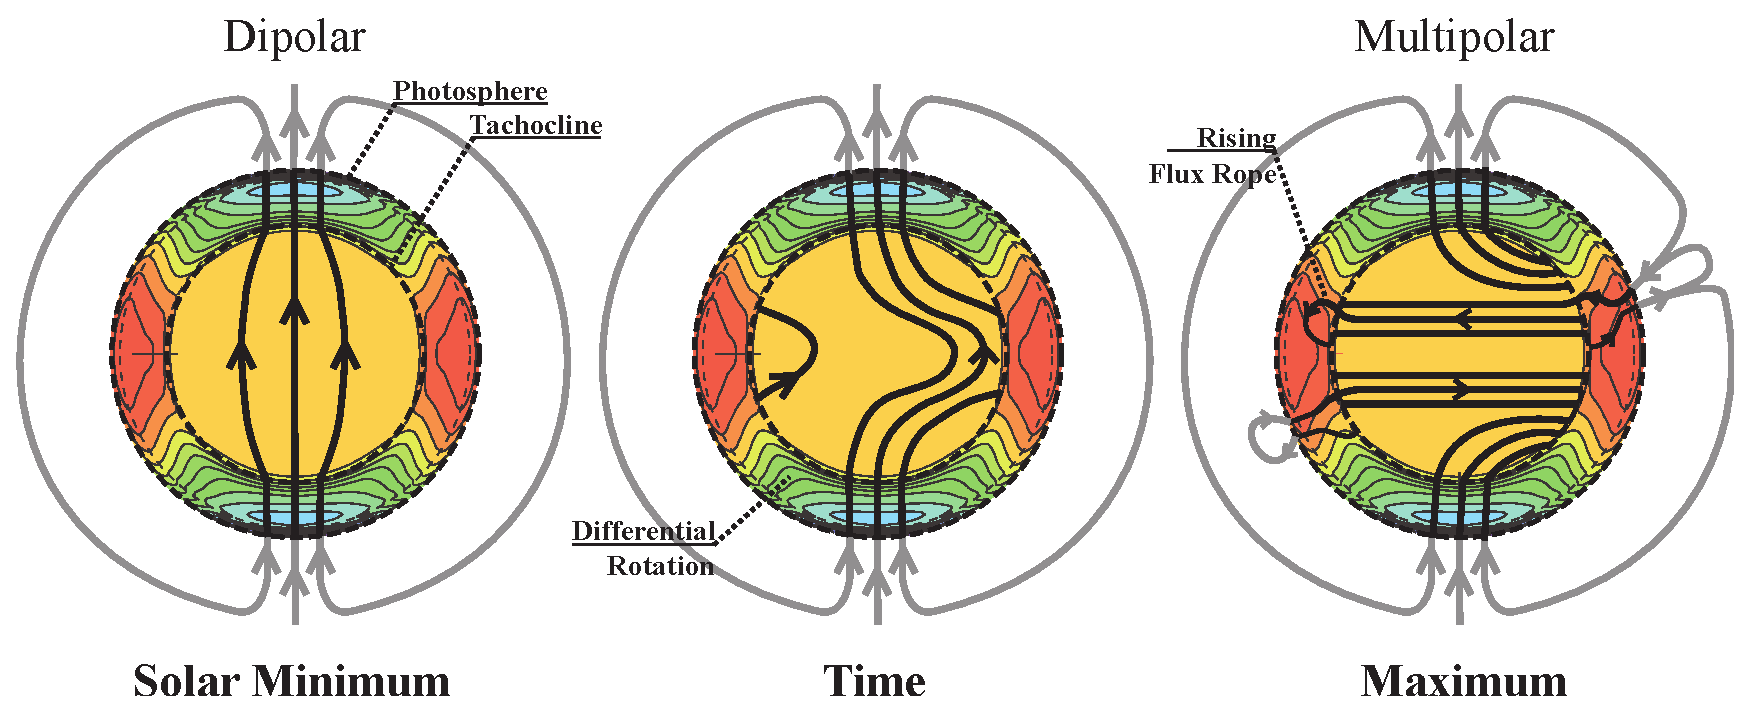
\includegraphics[width = 1.0\textwidth,clip=1]{dynamo_schem.eps}}
\caption[A summary of the magnetic solar cycle.]{A summary of the global magnetic field evolution between solar minimum and maximum. \emph{Left:} The global field is a dipole at solar minimum. \emph{Center:} Differential rotation results in dipolar field lines becoming toroidal. \emph{Bottom:} Flux ropes rise and emerge at the photosphere as sunspot groups.}
\label{fig:globalsummary}
\end{figure}

A $\sim$22\,year cycle is observed which includes two sunspot cycles. When this cycle begins at ``solar minimum", characterized by a minimum in the rate of sunspot emergence,  the global magnetic field is bipolar with magnetic north matching the spin-axis north pole. The global dipolar field lines are then displaced longitudinally and stretched into a toroidal configuration due to differential rotation, in which the rotational angular velocity of the Sun decreases with latitudinal distance from the equator. As the global bipolar field becomes toroidal, the polar magnetic field strengths decrease and a sharp increase in the number of emerging sunspots is observed. For several years during sunspot maximum, the global dipole switches polarity and the spin-axis north pole becomes magnetic south. Over the course of the next $\sim$6\,years, the rate of sunspot emergence decreases to a new minimum and the second half of the 22~year cycle follows, similar to the first, but with a flipped global dipole. The process from solar minimum to maximum is illustrated in Figure\,\ref{fig:globalsummary}.

%By tracking many magnetic flux elements over an entire solar cycle we aim to determine the precise characteristics of this flow.
%The likely candidate for carrying magnetic flux to the poles, resulting in reversal, is the meridional flow which is observed to originate at the equator and flow in either direction, poleward. 
It is commonly understood that during the solar cycle the polar fields are reversed by the accumulation of weak magnetic flux elements at high latitudes, carried from lower latitudes \citep{Babcock:1961, Leighton:1964}. It is thought that the combination of Joy's Law, the poleward meridional flow, and supergranular diffusion allow this process to occur \citep{Mosher:1977}. Small flux concentrations are carried to the poles more swiftly (than would be due to their diffusive random walk alone) by the meridional flow. The meridional flow itself has been indirectly measured using both surface tracking methods and helioseismology techniques \citep{Hathaway:2010,Haber:2002,Zhao:2004}. Since following (leading) flux concentrations in bipoles tend to be weaker (stronger), they are more affected by flows \citep{Schrijver:1996}. Thus slightly more (less) of the flux of the following (leading) polarity will random-walk to the nearest hemispheric pole before completely decaying. The process has been studied extensively by directly observing large scale quiet-Sun magnetic fields \citep{Harvey:1992,Ulrich:2005,Schrijver:2008b} and by using surface flux transport models \citep{Leighton:1964,Wang:1989,Schrijver:2003}. These models are able to qualitatively reproduce the evolution of the distribution of photospheric magnetic fields on the Sun. 

\citet{Ulrich:2002} shows that the global dipole field reversal is driven by the bursty emergence and poleward migration of ARs over a short period of time, rather than a continuous flux emergence process. The meridional flow latitude profile has been measured using Doppler data \citep{Ulrich:2005}, surface feature tracking methods \citep{Hathaway:2010}, and helioseismology techniques \citep{Haber:2002,Zhao:2004}. Each study presents observations of a reverse of direction in the meridional flow at high latitudes at different phases in the solar cycle. \citet{Schrijver:2008b} use measurements of the dipole strength and surface flux transport modeling to conclude that this dynamic meridional flow is responsible for cycle to cycle differences in the polar field strengths.

%EQN Dipole moment/Quadrupole moment etc
The imbalance of net magnetic flux is an observational effect resulting from summing the signed magnetic flux within a limited surface area on the Sun. It is important in the analysis of the large-scale magnetic field. Hemispheric flux imbalance, the magnetic polarity imbalance between the North and South hemispheres, affects the structure of the global magnetic field. For instance, a purely dipole field results from having a single opposing polarity in each hemisphere. In reality, the Sun's field is multipolar.
%4.1-hemispheric imbalance must be open flux or faraway conection. likely not trans longitude, probably trans hemisphere
Large scale measurements of the imbalance between outward (positive) and inward (negative) directed magnetic flux from 1975-2000 have been studied by \citet{Choudhary:2002} and it is seen that hemispheric flux imbalance is a function of the solar cycle and furthermore switches sign between cycles. A clear signal is found in the northern hemisphere, but is much less clear in the southern. Upon measuring flux imbalance in individual ARs, a larger percentage imbalance is found than that determined hemispherically. It is reasoned that this indicates ARs must be balanced by long-range connections to oppositely imbalanced ARs at similar latitudes and the hemispheric imbalance is resolved by trans-equatorial connections. If ARs were balanced using trans-equatorial connections then the hemispheric imbalance could be much larger.

\begin{landscape}
\begin{figure}
\centering{\includegraphics[width = 1.2\textwidth]{hath_bfly.eps}}
\caption[The sunspot cycle over $\sim$150\,years.]{The sunspot cycle over $\sim$150\,years \citep[from][]{Hathaway:2010b}. \emph{Top}: the number of sunspots at each latitude over time. This plot exhibits the characteristic butterfly shape. \emph{Bottom}: the total number of sunspots over time. The 11-year cycle is seen to occur with a varying peak sunspot number.}
\label{fig:sunspotnum}
\end{figure}
\end{landscape}

%%%%%%%%%%%%%%%%%%%%%%%%%%%%%%%%%%%%%%%%%%%%
\subsection{Global Field Reversal}\label{intro:fieldreversal}

The large-scale configuration of the magnetic field within the convection zone is thought to transition between being poloidal and toroidal, every 11\,years \citep{Parker:1955}. The process which facilitates this reorganisation is the magnetic dynamo. Longitudinal flows drag poloidal fields into a toroidal configuration and meridional flows then help to reverse the process. The poloidal field is measured at the North and South poles of the Sun during solar minimum \citep{Harvey:2002}. The large-scale toroidal field has also been directly measured by taking advantage of line-of-sight magnetic field measurements at the solar limb \citep{Ulrich:2005}. Toroidal fields at the tachocline are stretched into thin twisted flux ropes by shearing at the interface of the rigidly rotating radiative zone and regions where the differentially rotating convection zone is moving at a different speed. Turbulent perturbations introduce instability into the flux ropes and magnetic buoyancy becomes important and causes them to rise toward the surface, as described in Section \ref{intro:aremerge}.

%FLUX TRANSPORT MODELS
The combination of these phenomena causes a reversal of the polar magnetic fields \citep{Babcock:1961,Leighton:1964}. The Babcock-Leighton process can be seen in large-scale magnetogram observations \citep{Harvey:1992} and successfully reproduced using surface flux transport models \citep{Wang:1989,Schrijver:2003}. These models imply a buildup of net magnetic flux (an imbalance of $+$ and $-$ magnetic polarities) should occur at mid to low latitudes of the same polarity as the pole in that hemisphere. At higher latitudes, flux of one polarity builds up as magnetic elements are swept poleward. Low latitude flux from opposite hemispheres eventually diffuses toward the equator and cancels or submerges. Since net flux must sum to zero globally, one should measure the same magnitude, but opposite sign, of net flux at high and low latitudes in each hemisphere. For the first time we present a quantitative comparison of the amount of imbalanced flux in the AR bands and at high latitudes (Section \ref{subsect_imbharm}).
Regardless of the vehicle for flux decay and redistribution, the total observed flux decreases but physically the net flux must be conserved due to the solenoidal constraint (Gauss' Law), as there are no magnetic monopoles ($\nabla\cdot\mathbf{B}=0$).
Locally on the Solar surface, non-zero positive (negative) net flux may exist as it may be connected to distant negative (positive) flux concentrations, or may be quasi-open (connected to the solar wind) and balanced by other quasi-open negative (positive) flux concentrations on the solar surface.

%BUTTERFLY DIAGRAM
Latitudinal observations of net flux over time show that while the active region belt progresses from high to low latitudes, net unipolar flux is observed to be transported poleward, as observed in magnetic butterfly diagrams \citep{Harvey:1992}. \citet{Choudhary:2002} investigate large-scale flux imbalances finding that the signed flux imbalance between the North and South hemispheres is a function of the solar cycle and furthermore switches sign between cycles. \citet{zharkov:2006} study flux imbalance in individual sunspot groups statistically for a portion of solar cycle 23. Opposite imbalances in each hemisphere are found that reverse at the solar minimum. \citet{Zharkov:2008} state that a phase relation exists between active region flux imbalances and the background high-latitude magnetic field. These results support the Babcock-Leighton model.

%EQN Dipole moment/Quadrupole moment etc
The properties of detected ARs, such as flux imbalance, affect the solar magnetic structure locally, while on a global scale, hemispheric flux imbalance affects the structure of the solar magnetic field. For instance, a purely dipole configuration results from having a single opposing polarity in each hemisphere. 
\citet{mordvinov:2007} determines a relationship between the IMF and global field harmonic modes-- especially the $[l=2,m=0]$ mode.
Generally, the global field is multipolar and we can describe its structure extending into the solar atmosphere using the superposition of spherical harmonics, with a potential field source surface (PFSS) model. 

Some studies focus on periodicities in the harmonic coefficients over multiple solar cycles finding separate frequencies in axisymmetric and non-axisymmetric modes \citep{stenflo:1986, stenflo:1988, knaack:2005}.
It has been determined that to accurately predict the magnetic field at Earth, the properties of low latitude magnetic features on the Sun must be taken into account \citep{schussler:2006, wang:2003a, Schrijver:2003}. The distribution of open flux and the global field configuration determine the shape of the heliospheric field and thus can affect the space weather environment at Earth.
Taking these findings into account, we seek to better understand the evolution of the global solar magnetic field in the context of a full 11\,year activity cycle (half of a magnetic cycle) by characterizing spatio-temporal distributions of magnetic feature properties.

%%%%%%%%%%%%%%%%%%%%%%%%%%%%%%%%%%%%%%%%%%%%
\subsection{Active Sunspot Groups}\label{intro:flareactreg}

%Sunspot groups are formed by the convective action of sub-surface fluid motions pushing magnetic flux tubes through the Sun's surface, the photosphere. Turbulent photospheric and sub-photospheric motions jostle around these flux tubes and, when the conditions are right, the sunspot group produces a flare \citep{Conlon:2010a}. 
Sunspots are formed beneath the solar surface and emerge through the photosphere and into the corona. Turbulent photospheric and sub-photospheric motions jostle around the constituent flux tubes of the flux ropes that form sunspots, possibly resulting in destabilisation that leads to a flare \citep{Conlon:2010a}. Other phenomena, such as shearing and helicity injection, may build up stress in an AR leading to strong electric currents that correlate with flaring \citep{Schrijver:2005,Schrijver:2007}. 
Currently the exact conditions that are necessary for or lead to flaring are not known. This is partly due to limitations in our observational capabilities. Only the magnetic fields at the foot points of sunspot groups can be imaged, while flares actually occur some distance above the sunspot in the solar atmosphere. Flaring sunspot groups tend to be big and ugly (and thus bad). The largest eruptions and flares are released by large but compact sunspot groups with complicated magnetic configurations. In this section we will refer to active magnetic structures, including sunspot groups, as ``active regions" to include the entire system (surrounding magnetic flux elements and loop structures in the corona) connected to a flare.

\begin{figure}[!t]
\centerline{\includegraphics[width = 0.7\textwidth,clip=1]{McIntosh_1990_class.eps}}
\caption[The McIntosh sunspot group classification system.]{The McIntosh sunspot group classification system \citep[from][]{McIntosh:1990} The left column depends on the presence of spot penumbrae and group length. The middle column indicates features of the largest spot's penumbra. The right column is determined by the amount of spot coverage between the leading and trailing edges of the group.}
\label{fig:mcintoshclass}
\end{figure}

Several classifications of active regions were designed to describe alternatively white-light and magnetogram observations of sunspot groups. The most common, McIntosh classification (Figure~\ref{fig:mcintoshclass}), is an expansion of the Zurich system. It describes the number and development of sunspots within a group, including properties of umbrae and \glspl{penumbra}. \cite{McIntosh:1990} finds that the scheme is adept at indicating the relative flare productivity of a given class. 

The Hale classification system classifies the distribution of polarities in the active region, as described by Table~\ref{fig:haleclass}. This system has been expanded to include the $\delta$-class, which is given when two polarities are present within a single sunspot \gls{penumbra} \citep{Kunzel:1960}. The $\alpha$ indicates only one polarity of spot is visible, with p (f) meaning that any spots precede (follow) the magnetic field distribution. The $\beta$ indicates both spot polarities of spot are visible with p and f indicating which spot is larger. The $\gamma$ indicates spots of one polarity are on both sides of one or more spots of opposite polarity. Sunspot groups denoted as $\delta$-class are shown to produce the most significant flares \citep{sammis:2000}. These classification schemes are well correlated to quantitative descriptions of active region complexity \citep{ireland:2008}. 

%\begin{figure}[!t]
%%\centerline{\includegraphics[width = 0.5\textwidth]{images/hale_class.pdf}}
%\caption{...}
%\label{fig:haleclass}
%\end{figure}
\begin{table}[!t]
\caption[The possible sunspot group classifications using the Hale scheme.]{The possible sunspot group classifications using the Hale scheme \citep{Hale:1919} with the appended $\delta$-class \citep{Kunzel:1960}. The ``p" (``f") denote whether the strongest spot is preceding (following).}
\centering{
\begin{tabular}{lll}
\hline \hline
Unipolar & Multipolar & Mixed \\
\hline
$\alpha$ & $\beta$ & $\beta\delta$ \\
$\alpha$p & $\beta$p & $\beta\gamma\delta$ \\
$\alpha$f & $\beta$f & \\
& $\beta\gamma$ & \\
\hline
\end{tabular}
}
\label{fig:haleclass}
\end{table}

%REORGANISE THESE PARAGRAPHS INTO property types
Classification has been shown to be useful for grouping active regions by their expected flare productivity. The quantification of active region properties allows a physical comparison and deeper understanding of the actual causes flaring. Complexity, often quantified by fractal index \citep{mcateer:2005b,Conlon:2008,Conlon:2010a} and scale-power distributions \citep{Abramenko:2005,Hewett:2008} is shown to be correlated with flare productivity. However, recent work has shown that fractal dimension is not a good flare predictor \citep{georgoulis:2012}. 
The presence of shear and helicity injection are shown to initiate flaring within active regions \citep{Schrijver:2008a}.
Strong polarity separation lines with large gradients and large field magnitudes on either side are known to be one of the best indicators of flaring \citep{Schrijver:2007}.

Generally active regions emerge up to a certain size while their non-potential characteristics (such as polarity separation line strength) continue to evolve. Upon reaching a state of maximum complexity, active regions are observed to produce the most significant flares. The relationship between flux and the sum of magnetic gradients along a polarity separation line (\gls{wlsg}) is shown to be a power law \citep{Falconer:2009}. 

Various statistical methods have been used in conjunction with an assortment of physical properties to forecast flares. %Much work has been done using these properties to forecast flares (Section \ref{intro:flareforecast}).
Current forecasting systems are limited \citep{Messerotti:2009} and often generate incorrect predictions. The inaccuracy of forecasting systems may be very costly. Depending on the application, false alarm forecasts may result in lost revenue during satellite shut-downs, diverting trans-polar flights, delayed spacecraft launches. On the other hand, missed flares could result in damage to sensitive space-born instruments, such as those on communications, scientific, or military satellites, or the endangerment of pilots on transpolar flights and astronauts on space-walk \citep{national2008Severe}. In 1989 a solar storm caused disruptions to power grids in Quebec, the northeastern United States, and areas of Sweden causing blackouts for hours. Recently, communications with the civilian Galaxy 15 satellite were compromised in April 2010, and the spacecraft was unable to respond to commands from the ground for months. As our society and military become increasingly technologically advanced, we become more directly affected by solar activity.

Past work on predicting the occurrence of flares in sunspot groups has focused on determining a set of sunspot group properties important for flaring \citep{Gallagher:2002}. This requires a large set of characterized sunspot group detections, which is used to train a prediction system. Automated detection and characterization systems, such as the SolarMonitor Active Region Tracker \citep[SMART;][]{higgins:2011} developed by our team, are useful for this task and often focus on characterizing magnetic field properties. Using these detection methods, modules may be applied to determine various properties: size; magnetic flux; polarity separation line length; magnetic energy; magnetic connectivity. The sunspot group detections are then associated with a flare catalog and correlations are determined for specific properties and various prediction time windows and latencies.

There have been many studies attempting to find the most significant sunspot group properties for predicting flares. \cite{Leka:2003a,Leka:2003b,Leka:2007} and \cite{Barnes:2006} test a large number of vector magnetic properties (e.g., moments of the vector magnetic field, magnetic shear, and current helicity) in various combinations and find that characterizing a sunspot group at one point in time has limited bearing on whether it will flare in the future. 

More recent work, such as \cite{Colak:2009} and \cite{Ahmed:2011} rely on machine learning algorithms with a database of sunspot group descriptors and knowledge of flare occurrence as input. Much more accurate flare prediction results are achieved, while much fewer properties are investigated than previous studies.  \cite{Colak:2009} rely on automated McIntosh sunspot classifications as a sunspot descriptor that are generated using machine learning to make predictions. Alternatively, \cite{Ahmed:2011} use the line-of-sight magnetic properties defined in \cite{higgins:2011} and listed in Tables\,\ref{tablemagprop} and \ref{tablehighorder}. The descriptors with the most predictive power were found to be \gls{PSL} length ($L_{PSL}$), strong gradient \gls{PSL} length ($L_{sg}$), maximum horizontal magnetic field gradient ($(\nabla B)_{max}$), the sum of the gradient along $L_{sg}$ ($WL_{sg}$), the sum of the gradient along $L_{PSL}$ ($WL^*_{sg}$), and the total magnetic flux near the \gls{PSL} ($R^*$).

Using a completely different approach, \cite{Wheatland:2005} achieves good results predicting flares on the assumption that if a flare has occurred, more will occur. This shows that the history of activity of a sunspot group is a significant predictor. For the purposes of reliable operational forecasting, all existing systems are still limited, as their use results in substantial numbers of false alarms and missed flares. 

Most studies use point-in-time detections of sunspot groups to predict flares. \cite{Mason:2010} are an exception, and show promise in predicting flares using previous changes in magnetic properties. %Figure 2 shows the magnetic evolution of a tracked sunspot group as compared with its flare productivity. 
The concept of relating sunspot group dynamics and evolution has not been extensively explored.

%\begin{table}
%\caption{The observation-prediction contingency table, or affectionately as the ``confusagram". }
%\centering{
%\begin{tabular}{c|c|c}
%\hline \hline
%& Observed & Not Observed \\
%\hline
%'Yes' Forecast & TP & FP \\
%\hline
%'No' Forecast & FN & TN
%\end{tabular}
%}
%\label{table:conttable}
%\end{table}

%To compare the effectiveness of these forecasting systems several accuracy and skill scores have been appropriated from the climate sciences. These are calculated using a contingency table, as shown in Table~\ref{table:conttable}. Flare truth indicates whether or not a flare actually occurs, while forecast indicates whether one was predicted to occur. The elements of the table are true positives (TP) when a flare has occurred and was predicted, false negatives (FN) when a flare has occurred but was not predicted, true negatives (TN) when no flare has occurred and none was predicted, and false positives (FP) when no flare has occurred but one was predicted to occur. 
%Common forecast validation measures are, 
%\begin{eqnarray}
%accuracy &=& \\
%probability of detection &=& \\
%false alarm rate &=& \\
%heidke skill score &=& \\
%true skill statistic &=& \\
%\end{eqnarray}

%REF wilcox 1973? balch?

%%%%%%%%%%%%%%%%%%%%%%%%%%%%%%%%%%%%%%%%%%%%
\section{Solar Eruptions}\label{intro:solerupt}
%%%%%%%%%%%%%%%%%%%%%%%%%%%%%%%%%%%%%%%%%%%%

Solar eruptive activity is associated with large complex sunspot groups. The solar activity cycle is mainly observed by monitoring the number of sunspots on disk (sunspot number). On $\sim$year timescales the number of eruptive events observed is well correlated with the sunspot number. Each eruption is different and there are a wide variety of phenomena that are generally associated with them. To present a common scenario: often, as a sunspot group evolves, material can cool and collect in a ``channel", suspended above by the magnetic loop structure along a sheared \gls{PSL}. This material is called a filament or prominence depending whether it is observed from above or side-on. The shear and twist in the system introduces magnetic stresses. At some point an instability occurs and the fields are thought to rapidly reorganise to a lower energy state. Theoretically, this reorganisation releases part of the stored magnetic energy as radiation and non-thermal particle acceleration \citep{Fletcher:2011}. This conversion and release of energy is called a flare. The converted magnetic energy is considered to be part of the ``non-potential" portion of the magnetic energy in the system, as discussed in Chapter~\ref{chapter:theory}. Often this is accompanied by the release and acceleration of matter called a \gls{CME} which carries another large portion of the energy. The kinetic \gls{CME} energy has been shown to be greater, but of the same order of magnitude as the radiative flare energy \citep{Emslie:2004}. The accelerated matter generally includes filament material forming the ``core" and an overarching twisted magnetic loop structure called a flux rope forming the ``front" of the \gls{CME}. 

\begin{figure}[!t]
\centerline{\includegraphics[width = 0.7\textwidth,clip=1]{1_introduction/figures/flare_phases.eps}}
\caption[The progression of a typical solar flare.]{The progression of a typical solar flare \citep[from][]{Qiu:2009}. \emph{Top:} the impulsive phase is characterised by a rapid burst of hard X-rays (HXT), followed by the gradual decay of soft X-rays (GOES). \emph{Bottom left:} The contours indicate the location of HXR emission. \emph{Bottom right:} During the course of the flare, the foot points move apart, as indicated by the colored marks.}
\label{fig:flarephase}
\end{figure}

Solar flares are among the most energetic events occurring in the solar system, influencing a panorama of physical systems: from the solar surface and atmosphere, through the heliosphere, and into geo-space. Flares, along with coronal mass ejections, are a major contributor to space weather:  the interaction of magnetic fields and particles accelerated on or near the Sun with the Earth's magnetosphere and upper atmosphere. Although significant progress has been made in understanding the fundamental physics of flares, their accurate forecasting remains impossible.

Flares occur in volumes of the atmospheric plasma above sunspot groups with increased emission at temperatures of 1\,000\,000\,K or more. There are many flare cartoons which mainly rely on the release of magnetic energy through reconnection\footnote{See: \url{http://solarmuri.ssl.berkeley.edu/\~hhudson/cartoons/}.}. 
%During reconnection, large currents lead to heating which is observed at the tops of coronal loops. Additionally, particles stream down the loop legs, resulting in heating at their foot points in the chromosphere. 
%If the process is attributed to reconnection a ``breakage" of field lines occurs and acceleration of a plasmoid. This plasmoid can become a \gls{CME}. Often a filament lies over the flaring structure and subsequently lifts off, becoming the core of a \gls{CME}. 
It is thought that magnetic reconnection occurs at strong current sheets where magnetic fields are oppositely aligned, causing particle acceleration. Their occurrence tends to be along polarity separation lines \citep{Schrijver:2007}. High-energy particles stream down the legs of the reconnecting structure, impacting the chromosphere, and producing \gls{EUV} and X-ray radiation. High energy X-ray, or \gls{HXR}, emission is concentrated at the foot points and the apex of the structure near the reconnection region. Lower energy, or \gls{SXR}, emission is focused in different regions depending on the phase of the flare evolution, but is generally more widely distributed over the loop structure.

\begin{figure}[!t]
\centerline{\includegraphics[width = 0.7\textwidth,clip=1]{1_introduction/figures/aschwan_flare_freq.eps}}
\caption[The frequency distribution of flare magnitudes measured in various studies.]{The frequency distribution of flare magnitudes measured in various studies \citep[from][]{Aschwanden:2011}.}
\label{fig:flaredist}
\end{figure}

There are several stages in the evolution of a flare: the pre-flare, impulsive, and gradual phases \citep{Fletcher:2011}. The behaviour of emission at different wavelengths and the motions of the flare foot points is shown in Figure~\ref{fig:flarephase}. In the pre-flare phase, heating occurs that signals the oncoming flare. This often takes the form of a filament activation that is observed as a brightening of filament material in H-$\alpha$ observations. During the impulsive phase, rapid brightenings in \glspl{HXR} and radio (type III bursts) are observed. The main brightening in \gls{SXR} occurs more slowly and its peak divides the impulsive and gradual phases. During the initial \gls{SXR} brightening and peak, the shape of the time profile of \gls{HXR} emission generally follows the time derivative of the \gls{SXR} emission. This is called the Neupert effect and is thought to occur because the cooling timescale of coronal \gls{SXR} emitting plasma is longer than that of the chromospheric heating mechanism. Electrons accelerated during the flare cause non-thermal \gls{HXR} emission and chromospheric ``evaporation" that heats the corona above, resulting in thermal \gls{SXR} emission. This effect was first noted by \cite{Neupert:1968} by comparing X-ray and microwave observations.

\begin{table}
\caption[The GOES flare classification scheme.]{The GOES flare classification scheme, where peak fluxes are integrated over the 1-8\,\AA\ bandpass.}
\label{tab:gclass}
\centering{
\begin{tabular}{lc}
\hline \hline
Class & Peak Flux [W\,m$^{-2}$] \\
\hline
X10 & $10^{-3}$ \\
X & $10^{-4}$ \\
M & $10^{-5}$ \\
C & $10^{-6}$ \\
B & $10^{-7}$ \\
A & $10^{-8}$ \\
\hline
\end{tabular}
}
\end{table}

Large flares release around $10^{32}$\,erg of energy through radiation. They are often characterised by the magnitude of their peak emission in \glspl{SXR} using a 1-8\,\AA\ bandwidth. This classification system is a base-ten magnitude system called the GOES Class after the instrument used to define it and is summarised by Table~\ref{tab:gclass}. Each higher class of flare exhibits peak SXR emission ten times greater than the last. With in a single class, flares are usually ordered by the first two significant digits of their flux. For example, a flare with a peak flux of $4.5\times10^{-5}$\,W\,m$^{-2}$ would be given a classification of M4.5. The frequency flare occurrence with increasing magnitude follows a decreasing power law. A slope between -1.5 and -2.5 is measured in various studies \citep[see Figure~\ref{fig:flarephase};][]{Aschwanden:2011}. 
Also, the distribution of waiting times between flares over long time-scales has been shown to be a power law over time-scales greater than a few hours, pointing to an avalanche model \citep{Lu:1993}, but is exponential when considering the statistics over multiple solar cycles, indicating flaring is a random Poisson process \citep{Wheatland:2000}. Individual active regions exhibit an exponential distribution of flaring rates \citep{Wheatland:2001} and it is well known that the best predictor for a flare to occur in the future is that a flare has occurred in the past \citep{Wheatland:2005}.

%%%%%%%%%%%%%%%%%%%%%%%%%%%%%%%%%%%%%%%%%%%%
\section{Thesis Aims}\label{intro:aims}
%%%%%%%%%%%%%%%%%%%%%%%%%%%%%%%%%%%%%%%%%%%%

Very few sunspot-related phenomena are well understood. It is only superficially known how the large-scale plasma circulation and the decay and dispersion of sunspot magnetic fields are connected to the reversal of the global magnetic field. Above the photosphere, the magnetic field strength and structure can only be roughly estimated, and below the photophere neither is known to any certainty. Additionally, predicting the strength of the next solar cycle, sunspot emergence, and the occurrence of flares with the accuracy required by the operational community is not possible. 

The aim of this thesis is to better understand the evolution of individual sunspot groups and the global magnetic field. The study aims to address three questions in a series of studies:
\begin{itemize}
\item \emph{What are the conditions in sunspot groups that result in solar flares?} The relationship between flaring and sunspot group property dynamics is investigated. Property distributions associated with different flare magnitudes are compared. The properties of sunspot groups over the solar cycle are compared to global flare productivity. 
\item \emph{What mechanisms determine the configuration of the global magnetic field and how does this relate to the solar dynamo?} The distribution of magnetic features affects the global magnetic field of the Sun. A comparison between the properties of sunspot groups and the global field configuration over solar cycle 23 is presented. 
\item \emph{What mechanisms govern the evolution and decay of sunspot groups?} A mechanism for the decay of sunsot groups is investigated by comparing a large-scale observation of magnetic field dispersion to a simulation. 
\end{itemize}
To allow a large-scale study of the solar magnetic field, a combination of image processing techniques is used to automatically detect, characterise, and track sunspot groups over time.

The remainder of this thesis is organised as follows.
The theory describing magnetic fields in a plasma is presented in Chapter~\ref{chapter:theory}. 
The magnetic field observations and other data used in the investigations are described (see Chapter~\ref{chapter:data}). 
The methods for automatically detecting and characterising sunspot groups are described in \ref{chapter:method_SMART}. 
Three scientific studies of the solar magnetic field follow in Chapters~\ref{chapter:results_activity}, \ref{chapter:results_global}, and \ref{chapter:results_diffusion}.
Finally, the main results and conclusions of the studies, including prospects for future work, are summarised in Chapter~\ref{chapter:discussion}.	% background information

	% this file is called up by thesis.tex
% content in this file will be fed into the main document

\chapter{Theory of Magnetic Fields in a Plasma} % top level followed by section, subsection
\label{chapter:theory}

\graphicspath{{1b_theory/figures/EPS/}{1b_theory/figures/}}

%Reset all glossary terms
\glsresetall

%ABSTRACT-----------------------------------------------------
\hrule height 1mm
\vspace{0.5mm}
\hrule height 0.4mm 
\noindent 
\\ {\it 
In this chapter, theories explaining the dynamics and energetics of magnetised plasmas are discussed. Electrodynamic, fluid, and plasma equations leading to magnetohydrodynamics are described. Also, magnetic fields in the solar atmosphere, the magnetic energy release in flares, and the quantification of surface fields are explained. This chapter summarises the background theory of ideas presented throughout this thesis.
}
\\ 
\hrule height 0.4mm
\vspace{0.5mm}
\hrule height 1mm 
\vspace{1.5cm}
%\newpage
%END ABS---------------------------------------------------------

%%%%%%%%%%%%%%%%%%%%%%%%%%%%%%%%%%%%%%%%%%%%
\section{Plasma Physics}
%%%%%%%%%%%%%%%%%%%%%%%%%%%%%%%%%%%%%%%%%%%%

The material composing the Sun can be described as a plasma, which is defined as a gas in which a significant fraction of atoms are ionised. This ionisation is due to the enormous temperatures and pressures in the Sun. The fraction of ionisation varies with location and is described by the Saha equation,
\begin{equation}
%\frac{n_{I+1} n_e}{n_I} = \frac{G_{I+1} g_e}{G_I} \frac{(2 \pi m_e k_B T)^{3/2}}{h^3} \exp\left( -\frac{\chi_I}{k_B T} \right) \mbox{ ,}
\frac{n_{i+1}}{n_i} = \frac{2 Z_{i+1}}{n_e Z_i} \frac{(2 \pi m_e k_B T)^{3/2}}{h^3} e^{( -\chi_i/k_B T)} \mbox{\,,}
\end{equation}
where, $n_{i}$ and $n_{i+1}$ are the number of ions in the ionisation state $i$ and $i+1$, respectively. The partition function of each state is given by $Z$ ($Z_{i} \approx 2$ and $Z_{i+1} \approx 1$), %$g_e=2$ for fermions, 
and $\chi_i$ is the ionisation energy for a given state.
For hydrogen this reduces to, 
\begin{equation}\label{eqn:saha}
\frac{(n^+/n)^2}{1-(n^+/n)}=\frac{4\times10^{-9}}{\rho} T^{3/2} e^{(-1.6 \times 10^5 / T)} \mbox{\,,}
\end{equation}
where $n^+$ is the number density of ions and $n$ is the summed number density of neutrals and ions, assuming macroscopic charge neutrality. This can also be written in terms of pressure,
\begin{equation}\label{eqn:sahap}
\frac{(n^+/n)^2}{1-(n^+/n)}=\frac{4\times10^{-9}}{\rho^{5/2}} {\frac{P\mu m_H}{k_B}}^{3/2} e^{(-1.6 \times 10^5 \rho k_B /\mu m_H P)} \mbox{\,,}
\end{equation}
Hydrogen transitions from nearly neutral to almost completely ionised over a narrow transition region in temperature centered at $\sim$10\,000\,K. This temperature occurs at outer layers of the solar convection zone. The Saha equation can not be applied in most of the solar atmosphere where local thermodynamic equilibrium does not hold. Also, in the core of the Sun, the pressure is so immense and the density so large that adjacent hydrogen atoms are close enough to effect each other's ionisation energies. Thus, in the core, the ionisation fraction approaches unity due to the added effect of ``pressure ionisation".
%Deep in the solar interior, this fraction approaches unity, due to the added effect of pressure ionisation, which is not taken into account by Equation \ref{eqn:saha}. 

The average random kinetic (thermal) energy for a plasma is given by,
\begin{equation}
\langle E \rangle = (3/2) k_B T \mbox{.}
\end{equation}
%while the random kinetic energy of electrons is given by,
%\begin{equation}
%\langle E \rangle = 1/2 k_B T_e \mbox{,}
%\end{equation}
%where $T_e$ is the electron temperature.
The charged particles of a plasma are in constant motion, striving to cancel charge imbalance locally. The electron plasma oscillation frequency due to this motion is given by,
\begin{equation}
\omega = \sqrt{\frac{n e^2}{m_e \epsilon_0}} \mbox{\,,}
\end{equation} 
where $e$ is the charge of an electron, $m_e$ is the mass of an electron, and $\epsilon_0$ is the permittivity of free space. In \gls{cgs} this can be written,
\begin{equation}
f_p = \frac{\omega_p}{2 \pi} = 9\,000 \sqrt{n_e} \mbox{\,,}
\end{equation}
where the result is in Hz. 

The Debye length is given by,
\begin{equation}
\lambda_D = \sqrt{\frac{\epsilon_0 k_B T_e}{e^2 n_e}}  
\end{equation}
This is the distance over which an electron's charge is ``felt" by other charged particles. An electron's electric potential falls off exponentially outside of its Debye sphere. The plasma parameter is, 
\begin{equation}
\Lambda = 4 \pi n \lambda_D^3 \mbox{\,,}
\end{equation}
and indicates the number of particles within a Debye sphere. If $\Lambda >> 1$, the plasma is strongly coupled (regarding collective effects), or weakly coupled if $\Lambda << 1$. Generally, strongly coupled plasmas are ``cold" and dense (as in white dwarf and neutron star atmospheres), while weakly coupled plasmas are diffuse and hot (as in solar and space plasmas).
In a ``collisional plasma"\footnote{Collisional plasmas include those in collisional equilibrium, such as the solar corona.}, the mean free path of particles within the plasma is small compared to the observational length scale\footnote{The observational length-scale determines the scale on which plasma phenomena are observed.} and is given by,
\begin{equation}
\lambda_{mfp} = 1/\sigma_{cs} n \mbox{\,,}
\end{equation}
where $\sigma_{cs}$ is the the collisional cross-section. For charged particles $\sigma_{cs}$ is much larger than for neutrals due to the Coulomb force,
%\begin{equation}
%\sigma_{cs} = \pi \left( \frac{e^2}{6\pi k_B \epsilon_0} \right) \frac{1}{T^2} \mbox{\,,}
%\end{equation}
%where $\sigma_{cs}$ is much larger for charged particles due to the Coulomb force,
\begin{equation}
F = \frac{1}{4\pi \epsilon_0}\frac{q_1 q_2}{r^2} \mbox{\,,}
\end{equation}
where $q_1$ and $q_2$ are the charges of each particle, and $r$ is the distance between the particles.
The collision frequency is,
\begin{equation}
\nu \approx \frac{\sqrt{2} \omega_p^4}{64 \pi n_e} \left( \frac{k_B T}{m_e} \right)^{-3/2} \ln \Lambda \mbox{\,,}
\end{equation}
where $n_e$ is the electron number density. 
In the absence of magnetic fields, disturbances in the plasma travel at the sound speed,
\begin{equation}
v_s = \sqrt{\frac{\gamma p}{\rho}} \mbox{\,,}
\end{equation}
where $\gamma$ is the ratio of specific heat at constant pressure ($C_P$) to that at constant volume ($C_V$).

Magnetic and electric fields are ubiquitous on the Sun. %because of the significant ionisation fraction. 
In general, these fields are governed by Maxwell's equations, the equations of electrodynamics,
\begin{eqnarray}
\nabla \cdot \vec{E} = \frac{1}{\epsilon_0}\rho_e & \mbox{ (Gauss's law),} \\
\nabla \cdot \vec{B} = 0 & \mbox{ (solenoidal constraint),} \\
\nabla \times \vec{E} = -\frac{\partial \vec{B}}{\partial t} & \mbox{ (Faraday's law),} \\
\nabla \times \vec{B} = \mu_0\vec{j} + \mu_0 \epsilon_0 \frac{\partial \vec{E}}{\partial t} & \mbox{ (Amp\'ere's law),}
\end{eqnarray}
where $\vec{E}$ is the electric field, $\vec{B}$ is the magnetic field, $\vec{J}$ is the current, $\rho_e$ is the charge density, $\epsilon_0$ is the permittivity of free space, and $\mu_0$ is the permeability of free space. The equation of motion for a charged particle traveling through electric and magnetic fields is,
\begin{equation}\label{eqn:lorenz}
m_e \frac{\partial^2 \mathbf{x}}{\partial t^2} = \vec{F} = \underbrace{q\vec{E}}_{\mathrm{Coulomb}}+\underbrace{q\vec{v}\times\vec{B}}_{\mathrm{Lorentz}} \mbox{\,,}
\end{equation}
where $q$ is charge of the particle and $\vec{v}$ is the velocity of the particle moving through the field. In Section~\ref{sect:mhd} dynamics will be described in terms of a magnetised fluid, rather than of a single particle.
 
The force on a charged particle due to a vertical magnetic field results in the particle revolving around the field in the horizontal plane. Considering an electron, the frequency at which this occurs is the electron gyrofrequency,
\begin{equation}
\omega_g = -\frac{e B}{m_e}  
\end{equation}
The gyroradius is then,
\begin{equation}
r_g = \frac{v_\bot}{\omega_g}  
\end{equation}
This motion results in gyro-synchrotron emission which is often observed in regions of strong magnetic field on the Sun at microwave wavelengths \citep{Gopalswamy:2012}. 
%From this description of the properties of a plasma, the plasma criteria are,
%\begin{eqnarray}
%\end{eqnarray}

%%%%%%%%%%%%%%%%%%%%%%%%%%%%%%%%%%%%%%%%%%%%
\section{Fluid Dynamics}
%%%%%%%%%%%%%%%%%%%%%%%%%%%%%%%%%%%%%%%%%%%%

In general, the Sun can be treated as a fluid. The fluid approximation allows one to model solar material as a continuous spatial distribution of fluid parcels, rather than a collection of particles. The principle fluid equations are,
\begin{eqnarray}
\label{eqn:mhdmasscont} \frac{\partial \rho}{\partial t}+\nabla\cdot(\rho \vec{v}) = 0 \mbox{ (mass continuity),} \\
\label{eqn:fluidmotion} \rho \frac{D \vec{v}}{D t} = -\nabla P + \vec{F} \mbox{ (equation of motion),} \\
\label{eqn:fluidenergy} \frac{D}{D t}\left( \frac{P}{\rho^{\gamma}} \right) = -\mathcal{L} \mbox{ (energy equation),} \\
P=\frac{\rho k_B T}{m_p \overline{\mu}} = n k_B T \mbox{ (ideal gas law),}
\end{eqnarray}
where $\vec{F}$ denotes external forces on the fluid, $\mathcal{L}$ is the total energy loss rate, $\gamma$ is the ratio of specific heats (of constant pressure to constant volume), $m_p$ is the mass of a proton, $\overline{\mu}$ is the mean molecular weight, and
\begin{equation}
\frac{D}{D t} = \frac{\partial}{\partial t}+\vec{v} \cdot \nabla
\end{equation}
is the convective time derivative. The mean molecular weight is $\sim$0.6 for ionised solar plasma, but for small ionisation fractions $\mu$ is $\sim$unity.

%VISCOUS / TURBULENCE -describes scales of convection?
The Reynolds number indicates whether the inertial or viscous forces in a fluid dominate. The Reynolds number is given by, 
\begin{equation}\label{eqn:magreynolds}
R_{e} = \frac{V L}{\nu_{visc}} = \frac{\rho V L}{\mu_{visc}} \mbox{\,,}
\end{equation}
where, $V$ is a characteristic velocity in the fluid, $L$ is a characteristic length scale of the system, $\rho$ is the fluid density, $\nu_{visc} = \mu_{visc}/\rho$ is the kinematic viscosity, and $\mu_{visc}$ is the dynamic viscosity, a measure of how much the fluid resists an applied shearing force. Turbulence becomes an important form of energy transport for fluids of Reynolds number ($R_{e}$) greater than $\sim$5\,000. In the convection zone and lower photosphere $R_{e}$ is many orders of magnitude larger than this; in the granulation layer it is estimated to be $\approx$10$^9$ \citep{Cox:1991}. Turbulent flows are highly disorganised and exhibit a cascade of energy to smaller scales. At the smallest scales the kinetic energy of the flows is dissipated as heat through molecular diffusion and viscosity. The turbulent heat flux is
\begin{equation}
H_{k} = v \rho C_{P} T \mbox{\,,}
\end{equation}
where $v$ is the speed of a turbulent fluctuation, $C_{P}$ is the specific heat at constant pressure, and $T$ is the temperature of the fluctuation. The turbulent length scale where energy is dissipated as heat (the Kolmogorov scale) is given by,
\begin{equation}\label{eqn:turbeta}
\eta_k = \frac{\nu^3}{\epsilon_k} \mbox{\,,}
\end{equation}
where $\epsilon_k$ is the rate of energy dissipation.

The distribution of energy with scale can be obtained by Fourier decomposing a given flow field and considering Equation~\ref{eqn:turbeta} and the scales of turbulence, $\eta_k << \ell_{k} << L$, where $\ell_{k}$ denotes the medium turbulent scales and $L$, the largest scales in the system. The scale of $\ell_{k}$ is defined somewhat arbitrarily, limited by the molecular scale $\eta_k$ and the observational length scale. The distribution of energy is then,
\begin{equation}
E(r) = C \epsilon_k^{2/3} k^{-5/3} \mbox{\,,}
\end{equation}
where $C$ is a universal scaling constant and the wavenumber, $k = 2\pi/\ell_{k}$. Kolmogorov thus derived a universal scaling law of $-5/3$ for the turbulent energy cascade over spatial scale. Many studies have tried to determine the scale dependence of features on the Sun \citep{Hewett:2008,parnell:2009}, relating their properties to turbulent phenomena.
%DISTRIBUTION OF KE
%On scales smaller than granulation, turbulence is important and results in an energy cascade over a range of scales. Kolmogorov described to distribution of energy with scale...He found a universal scaling of a power-law of $\alpha=5/2$.

%%%%%%%%%%%%%%%%%%%%%%%%%%%%%%%%%%%%%%%%%%%%
\section{Magnetohydrodynamics}\label{sect:mhd}
%%%%%%%%%%%%%%%%%%%%%%%%%%%%%%%%%%%%%%%%%%%%

To describe the dynamics of solar plasma, an electrically charged fluid, we utilize \gls{MHD}. This framework differs from electrodynamics in its fluid mechanics component. Maxwell's equations are altered using several assumptions. It is assumed that the plasma is in collisional equilibrium, which is true in the solar interior and lower atmosphere. It is also assumed that the plasma flow velocities are much less than the speed of light. 
%This may be measured from doppler shift observations, helioseisomology, and by applying local correlation tracking (LCT) to photospheric magnetograms. In the latter case, \cite{Chae:2001} finds horizontal surface flow velocities of $~$$0.15$~km~s$^{-1}$. 
We may then neglect the displacement current in Amp\'ere's law, which becomes,
\begin{equation}\label{amperes}
\nabla \times \vec{B} = \mu_0 \vec{j} \mbox{\,,}
\end{equation}
where $\vec{B}$, $\mu_0$, and $j$ are the magnetic field vector, magnetic permeability, and current density vector, respectively. Charge neutrality is also assumed, which implies that an electric field can only be induced by a changing $\vec{B}$ field and $\nabla\cdot \vec{E}=0$, since excesses of charge are not allowed to accumulate. Faraday's law governs this induced electric field,
\begin{equation}\label{faradays}
\frac{\partial \vec{B}}{\partial t} = - \nabla \times \vec{E}  
\end{equation}
Currents are generated in the plasma by a non-zero $\vec{E}$ or a changing $\vec{B}$ and are determined using the generalized Ohm's law,
\begin{equation}  \label{ohms}
\vec{j} = \sigma(\vec{E} + \vec{v} \times \vec{B}) \mbox{\,,}
\end{equation}
where $\sigma$ and $\vec{v}$ are the electrical conductivity and plasma velocity, respectively. 
We can then solve for $\vec{E}$ in Equation~\ref{ohms} and substitute it into Equation~\ref{faradays},
\begin{equation}
\frac{\partial \vec{B}}{\partial t} = -\nabla \times \left( \frac{\vec{j}}{\sigma} - \vec{v}\times\vec{B} \right)  
\end{equation}
Thus, currents can be defined in terms of $\vec{B}$ alone.
Equation~\ref{amperes} is then rearranged and substituted for $\vec{j}$,
\begin{equation}\label{eqn:indprevecid}
\frac{\partial \vec{B}}{\partial t} = \nabla \times (\vec{v}\times\vec{B}) - \nabla \times \left( \frac{\nabla\times\vec{B}}{\mu_0 \sigma} \right)  
\end{equation}
A vector identity,
\begin{equation}\label{eqn:vecid11}
\nabla\times\nabla\times\vec{A}=\nabla(\nabla\cdot \vec{A})-\nabla^2\vec{A} \mbox{\,,}
\end{equation}
is then applied to the second term,
\begin{equation}
\frac{\partial \vec{B}}{\partial t} = \nabla \times (\vec{v}\times\vec{B}) + \nabla^2 \left( \frac{B}{\mu_0 \sigma} \right) - \cancel{ \nabla\times\left(\nabla\left( \nabla \cdot \frac{\vec{B}}{\mu_0 \sigma} \right)\right) } \mbox{\,,}
\end{equation}
where the third term is cancelled using the solenoidal constraint ($\nabla \cdot \vec{B}=0$). Simplification is performed by assuming $\sigma$ is constant and defining magnetic diffusivity, $\eta\equiv1/\mu_0 \sigma$,
\begin{equation}\label{induction}
\frac{\partial \vec{B}}{\partial t} = \nabla \times (\vec{v} \times \vec{B}) + \eta \nabla^2 \vec{B}  
\end{equation}
This is known as the ``induction equation", and is fundamental in explaining the creation and destruction of magnetic fields in plasmas.

The first term on the right-hand side is the advective term which describes magnetic field dynamics due to plasma flows, and the second is the diffusive term which describes diffusion of the field due to gradients in the magnetic field itself. The advective timescale (Equation~\ref{tadv}) is often much shorter than the diffusive (Equation~\ref{tdiff}), so flows tend to dominate the magnetic field dynamics. By dimensional analysis of Equation~\ref{induction}, characteristic timescales may be derived,
\begin{equation}\label{tadv}
\frac{\Delta \vec{B}}{\Delta t} = \frac{\vec{v}  \vec{B}}{\Delta l} ~\Rightarrow~
\tau_{adv} = \frac{\Delta l \Delta \vec{B}}{\vec{v}  \vec{B}} \mbox{\,,}
\end{equation}
\begin{equation}\label{tdiff}
\frac{\Delta \vec{B}}{\Delta t} = \eta \frac{\vec{B}}{\Delta l^2} ~\Rightarrow~
\tau_{diff}= \frac{\Delta l^2 \Delta \vec{B}}{\eta \vec{B}} \mbox{\,,}
\end{equation}
where $\Delta l$ is a characteristic length scale and $\Delta \vec{B}$ is the difference in magnetic field between the start and end of the time-scale which is roughly equivalent to the characteristic field, $\vec{B}$. 

When applied to a medium-sized sunspot at the photosphere, $\Delta l$ is of order 10\,Mm, $v$ is of order $10^{-4}$\,Mm\,s$^{-1}$, and $\eta$ is of order $10^{-9}$\,Mm$^2$\,s$^{-1}$. A $\tau_{diff}$ of $\sim$3\,000\,years and a $\tau_{adv}$ of $\sim$1\,day is determined. Sunspots are observed for days (the longest-lived last for months), not years; the advective term is clearly the more important for photospheric magnetic feature dynamics. Sunspot decay is thus due to convective (plasma flow) dispersion as discussed in \cite{Schrijver:2001}. Assuming the conductivity ($\sigma$) to be infinite results in ideal \gls{MHD}. In ideal MHD, Equation~\ref{induction} becomes,
\begin{equation}\label{idealind}
\frac{\partial \mathbf{B}}{\partial t} = \nabla \times (\vec{v} \times \vec{B})  
\end{equation}

The ratio of the diffusive and advective terms in the induction equation yield the magnetic Reynold's number,
\begin{equation}\label{eqn:reynum}
R_m = \frac{V L}{\eta} \mbox{\,,}
\end{equation}
where $V$ is a characteristic fluid speed and $L$ is a characteristic length scale.
This number indicates the relative importance of fluid motions to magnetic diffusion in the evolution of the magnetic field. In most cases for the Sun $R_m >> 1$, so the magnetic diffusion term in Equation~\ref{induction} can be neglected. There are a few cases where this is far from true, such as in flares. In Ideal \gls{MHD} the frozen-in condition applies and magnetic field lines are permanently embedded in the plasma they inhabit. Thus the field is advected with plasma motions or plasma is constrained to flow along field lines.

To complete the set of MHD equations, we rewrite the fluid equations, coupling some of them to the electrodynamic ones. Using the vector identity, 
\begin{equation}
\nabla\cdot(a\vec{A})=(\nabla a)\cdot \vec{A}+a(\nabla\cdot\vec{A}) \mbox{\,,} 
\end{equation}
we can rewrite Equation~\ref{eqn:mhdmasscont},
\begin{equation} 
\frac{\partial\rho}{\partial t}+(\vec{v}\cdot\nabla)\rho+\rho\nabla\cdot\vec{v} = 0  
\end{equation}
For an incompressible plasma, this becomes $\nabla\cdot\vec{v}=0$. Equation~\ref{eqn:lorenz} is substituted into Equation~\ref{eqn:fluidmotion} for $\vec{F}$, coupling the fluid and electrodynamic forces, 
\begin{equation}\label{eqn:mhdforce}
\rho\frac{D \vec{v}}{D t}=-\nabla P + \vec{J} \times \vec{B} + \rho \vec{g}  
\end{equation}
Assuming the fluid evolves adiabatically, no heat flows between fluid parcels and $\mathcal{L}=0$. Thus Equation~\ref{eqn:fluidenergy} and \ref{eqn:mhdmasscont} are combined to become,
\begin{equation}
\frac{\partial P}{\partial t}+\vec{v}\cdot\nabla P = -\gamma P \nabla \cdot \vec{v}  
\end{equation}

The energy density of a magnetic field is given by,
\begin{equation}
u_B = \frac{B^2}{2\mu_0}
\end{equation}
The total magnetic energy in a region of space is given by integrating over volume,
\begin{equation}
U_B = \int \limits_V \frac{B^2}{2\mu_0}\,dV  
\end{equation}
Considering the time evolution of the total energy and using a dot-product identity, 
\begin{equation}
\frac{d U_B}{d t} = \frac{1}{2\mu_0} \int \limits_V \frac{d}{dt}(\vec{B}\cdot\vec{B})\,dV  
\end{equation}
Using the product rule,
\begin{equation}
\frac{d U_B}{d t} = \frac{1}{2\mu_0} \int \limits_V \vec{B}\cdot\frac{d\vec{B}}{dt}+\frac{d\vec{B}}{dt}\cdot\vec{B}\,dV = \frac{1}{\mu_0} \int \limits_V \vec{B}\cdot\frac{d\vec{B}}{dt}\,dV 
\end{equation}
Equation~\ref{eqn:indprevecid} is then substituted for $d\vec{B}/dt$,
\begin{equation}
\frac{d U_B}{d t} = \frac{1}{\mu_0} \int \limits_V \vec{B} \cdot (\vec{\nabla} \times (\vec{v} \times \vec{B}) - \vec{\nabla} \times (\eta \vec{\nabla} \times \vec{B}))\,dV  
\end{equation}
The following equation can be derived from this by using a vector identity and substituting for current,
\begin{equation}
\frac{d U_B}{d t} = -\int \frac{j^2}{\sigma} dV - \int \vec{v} \cdot (\vec{j} \times \vec{B})\,dV  
\end{equation}
The left term represents energy lost through the dissipation of currents. This is also known as ohmic or Joule heating. The right term represents energy lost through work done on the plasma by the Lorentz force.

%INSERT MAGNETIC TENSIION AND PRESSURE FORCE DERIVATION
In addition to separating magnetic energy losses into components, the same can be done with magnetic forces. Combining Equation~\ref{amperes} and the Lorentz force in Equation~\ref{eqn:mhdforce} we can write, 
\begin{equation}
F_L = \frac{(\nabla\times\vec{B})\times\vec{B}}{\mu_0}  
\end{equation}
Using a vector identity (\,$(\vec{C}\times \vec{B})\times \vec{A} = \vec{A}\times (\vec{B}\times \vec{C})$\,) this can be rewritten,
\begin{equation}
F_L = \frac{\vec{B}\times(\vec{B}\times\nabla)}{\mu_0}  
\end{equation}
The force can then be split into two components using Equation~\ref{eqn:vecid11},
\begin{equation}
F_L = \underbrace{-\nabla \frac{B^2}{2\mu_0}}_{\mathrm{pressure}} + \underbrace{\frac{1}{\mu_0}(\vec{B}\cdot\nabla)\vec{B}}_{\mathrm{tension}}  
\end{equation}
Thus, the Lorentz force has a component acting perpendicular to the field, magnetic pressure\footnote{The magnetic pressure, $B^2/2\mu_0$ is numerically equivalent to the magnetic energy density.}, and a component acting along the field, magnetic tension. These forces can conveniently be attributed to many dynamic phenomena independently. Magnetic pressure is attributed to the apparent expansion of coronal loops as they reach higher into the atmosphere, while tension explains the restoring force that allows a coronal loop to spring back into place after it is disturbed by an external force. 

The dominance of fluid forces over electrodynamic forces can be determined from the ratio of gas pressure to magnetic pressure,
\begin{equation}\label{eqn:plasmabeta}
\beta = \frac{P_G}{P_B} = \frac{n k_B T}{B^2/2\mu_0}  
\end{equation}
In the solar interior $\beta>>1$ and magnetic fields dynamics are dominated by plasma motions, while in the corona $\beta<<1$ and magnetic fields determine plasma motion. In sunspots $\beta\sim1$, and the dynamics become very complicated.
%are advected with the plasma or are ``frozen in"

Magnetic tension and pressure are restoring forces that allow oscillations to take place along magnetic field lines. There are several types of waves that may occur.
Alfv\'en waves are incompressible transverse waves and only involve magnetic tension. The plasma motion due to the waves occurs perpendicularly to the wave vector and the magnetic field. The ``group" speed at which Alfv\'en wave energy travels along field lines is the Alfv\'en speed,
\begin{equation}
v_A = \frac{B}{\sqrt{\mu_0 \rho}} 
\end{equation}
When the ratio of gas to magnetic pressure, $\beta \ll 1$, then $v_A \gg v_s$. 
The phase speed of the wave pattern is given by,
\begin{equation}
\frac{\omega}{k} = \pm v_A \cos \theta \mbox{\,,}
\end{equation}
where $\omega$ is the angular frequency of the wave, $k$ is the wave vector, and $\theta$ is the angle between $B$ and $k$.
Alfv\'en waves allow for energy to be transported into the corona, as they are not affected by the acoustic cut-off frequency. They are thought to be partially responsible for the fast solar wind.

Magnetoacoustic waves come in two forms: ``fast" and ``slow". Fast waves propagate isotropically and are governed by magnetic pressure in media where $\beta \ll 1$ or by gas pressure when $\beta \gg 1$. The phase speed is given by,
\begin{equation}
v_{p,f} = \frac{\omega}{k} = \left( \frac{1}{2} (v_A^2 + v_s^2) + \frac{1}{2}\sqrt{(v_A^2+v_s^2)^2 - 4 v_A^2 v_s^2 \cos^2 \theta} \right)^{1/2} \mbox{\,,}
\end{equation}
where $v_s$ is the speed of sound in the plasma. For waves propagating parallel to $\mathbf{B}$, $v_{p,f}=v_A$ or perpendicular to $\mathbf{B}$, $v_{p,f}=\sqrt{v_A^2+v_s^2}$.
Slow waves mostly propagate along $\mathbf{B}$ and are governed by gas pressure when $\beta \ll 1$ or magnetic tension when $\beta \gg 1$. Their phase speed is given by,
\begin{equation}
v_{p,s} = \frac{\omega}{k} = \left( \frac{1}{2} (v_A^2 + v_s^2) - \frac{1}{2}\sqrt{(v_A^2+v_s^2)^2 - 4 v_A^2 v_s^2 \cos^2 \theta} \right)^{1/2}
\end{equation}
For waves propagating parallel to $\mathbf{B}$, $v_{p,s}=v_s$. They do not propagate perpendicular to $\mathbf{B}$.
%are longitudinal along field lines and involve both magnetic pressure and tension forces. These waves are governed by,
%\begin{equation}
%\frac{\omega}{k} = \left( \frac{1}{2} (v_A^2 + c^2) \pm \sqrt{(v_A^2+c^2)^2 - 4 v_A^2 c^2 \cos^2 \theta} \right)^{1/2} \mbox{\,,}
%\end{equation}
%where the case of addition results in fast magnetoacoustic waves and the case of subtraction results in slow waves. Fast waves occur when $c > v_A$ and slow waves if $c < v_A$.  

%%%%%%%%%%%%%%%%%%%%%%%%%%%%%%%%%%%%%%%%%%%%
\section{Dynamo Theory}
%%%%%%%%%%%%%%%%%%%%%%%%%%%%%%%%%%%%%%%%%%%%

\begin{figure}[!t]
\centerline{\includegraphics[width = 0.5\textwidth]{parkerglobalfield.eps}}
\caption[A schematic of magnetic fields generated by the solar dynamo.]{A schematic of the large-scale magnetic fields generated by the solar hydromagnetic dynamo. The thick lines represent bands of migrating toroidal flux in the convection zone. Thinner lines represent the ambient toroidal and poloidal field \citep[from][]{Parker:1957}.}
\label{fig:parkerdynamo}
\end{figure}

An important question in solar physics is how the large-scale magnetic field is generated. It is observed to change configuration over the solar cycle, so it must be time dependent. Also, sunspots are thought to be a manifestation of the large-scale field. The underlying process, responsible for the dynamic solar magnetic field and driven by internal flows, is called the dynamo. 
 
In general, the main goal of a dynamo theory is to solve the induction equation (Equation~\ref{induction}) for a given velocity and magnetic field. Assuming a velocity field within the Sun do to large-scale flows, 
\begin{equation}\label{eqn:dynamoflow}
v(r,\theta) = \underbrace{ \vec{u}_p(r,\theta) }_{\mathrm{meridional}} + \underbrace{ \overline{\omega} \Omega(r,\theta) \hat{e}_{\phi} }_{\mathrm{rotational}} \mbox{\,,}
\end{equation}
where $\vec{u}_p$ is the meridional (poloidal) flow, $\overline{\omega}=r\sin{\theta}$, and $\Omega $ is the solar rotation, a differential toroidal flow that varies with depth and latitude.
The magnetic field can be broken into a poloidal and toroidal component,
\begin{equation}\label{eqn:dynamofield}
\vec{B}(r,\theta,t) = \underbrace{ \nabla\times(A(r,\theta,t)\hat{e}_{\phi}) }_{\mathrm{poloidal}} + \underbrace{ B(r,\theta,t)\hat{e}_{\phi} }_{\mathrm{toroidal}} \mbox{\,,}
\end{equation}
where $A$ and $B$ are scalar functions that determine the field components.
%WHAT IS A?!?!?!
While the magnetic field varies with time, the large-scale flows are assumed to be static. Combining Equation~\ref{induction}, \ref{eqn:dynamoflow}, and \ref{eqn:dynamofield} we have a differential equation for the poloidal and toroidal components of the magnetic field,
\begin{equation}\label{eqn:dadt}
\frac{\partial A}{\partial t} = \eta \left( \nabla^2 - \frac{1}{\overline{\omega}^2}\right) A - \frac{\vec{u}_p}{\overline{\omega}} \cdot \nabla(\overline{\omega} A) \mbox{\,,} %& \mbox{ poloidal,} \\
\end{equation}
and,
\begin{equation}\label{eqn:dbdt}
\frac{\partial B}{\partial t} = \eta \left( \nabla^2 - \frac{1}{\overline{\omega}^2}\right) B + \frac{1}{\overline{\omega}} \frac{\overline{\omega}B}{\partial r}\frac{\partial \eta}{\partial r} - \overline{\omega}\nabla \cdot \left( \frac{B}{\overline{\omega}} \vec{u}_p \right) + \underbrace{ \overline{\omega}( \nabla \times (A\hat{\vec{e}}_{\phi}))\cdot\nabla\Omega }_{\mathrm{shear~term}} %\mbox{ .}%& \mbox{ toroidal.}
\end{equation}
where $\eta$ is the magnetic diffusivity. The shear term generates the toroidal field with a strength $\propto \nabla\Omega$.

Crowling's theorem says that an axisymmetric flow cannot generate an axisymmetric magnetic field. Also, a field with an electric current limited to a finite volume cannot be maintained by a flow with finite amplitude. The fields decay because of the finite conductivity (magnetic diffusivity term). Because of this, most dynamo models use an extraneous source term to initialise the field. 

\cite{Parker:1955} finds oscillatory solutions to Equations~\ref{eqn:dadt} and \ref{eqn:dbdt} in rectilinear coordinates that result in equatorward propagating dynamo waves. The waves take the form of bands of toroidal flux and are thought to explain the equatorward progression of sunspot group emergence over the solar cycle. A schematic of the process is shown in Figure~\ref{fig:parkerdynamo}. This result led to the formulation of many other dynamo models  \citep{Charbonneau:2010}.

In the ``mean-field" model, small scale turbulence leads to macroscopic fields. This leads to another term in Equation~\ref{induction} that is related to the curl of an electromotive force generated by the combination of the Coriolis force (large scale) and turbulent diffusion (small scale). The electromotive force is given by, 
\begin{equation}\label{eqn:epsmean}
\varepsilon = \alpha \vec{B} + \beta \nabla \times \vec{B} \mbox{\,,}
\end{equation}
where $\alpha$ is proportional to (negative) kinetic helicity and $\beta$ is related to turbulent diffusion. 
%By averaging the induction equation over space? we arrive at, ... (pg. 57 heliophys book 1) . The first term is the average electro motive force.
Here, $\alpha$ is a coefficient of the source term that results in the ``$\alpha$-effect" where,
\begin{equation}\label{eqn:alphamean}
\alpha = -\frac{1}{3} \tau_c \langle \vec{v}' \cdot (\nabla \times \vec{v}) \rangle \mbox{\,,}
\end{equation}
in units of m\,s$^{-1}$, where $\vec{v}'$ represents turbulent flows, $\vec{v}$ represents large-scale flows, and $\tau_c$ is the correlation time scale for the diffusion. The coefficient governing the turbulent source term is given by, 
\begin{equation}\label{eqn:betamean}
\beta = \frac{1}{3} \tau_c \langle {\vec{v}'}^2 \rangle \mbox{\,,}
\end{equation}
in units of m$^2$~s$^{-1}$. The time scale governing turbulent diffusion is,
\begin{equation}\label{eqn:taumean}
\tau_{diff} = \frac{R_{\odot}^2}{\eta_e} \mbox{\,,}
\end{equation}
where $\eta_e$ is the diffusivity, dominated by turbulence, rather than microscopic magnetic diffusion. Assuming a $\eta_e$ of 10$^8$\,m$^2$s$^{-1}$ and a length scale of 10$^8$\,m, the turbulent decay time scale for the Sun is $\sim$3\,years, which is of the same order of magnitude as the solar cycle length.
Equation~\ref{eqn:alphamean} and \ref{eqn:betamean} can be used to determine new equations for $\partial A/\partial t$ and $\partial B/\partial t$, with terms relating to magnetic induction due to the $\alpha$-effect and the ``$\Omega$-effect" (determined by the rotation of the convective zone), and magnetic diffusivity. 

A simplified model, the ``linear $\alpha$-$\Omega$ dynamo" neglects the meridional flow. Linear equations for $B$ and $A$ can be obtained leading to a dynamo wave equation. The direction of the waves is determined by,
\begin{equation}
\vec{s} = \alpha \nabla \Omega \times \mathbf{\hat{e}}_{\phi} \mbox{\,,}
\end{equation}
where $\Omega$ is the differential rotation profile and $\alpha$ is a coefficient determining the strength of the $\alpha$-effect, as before. At the high-latitude regions of the tachocline, $\nabla \Omega$ points radially inward. With a positive $\alpha$ this results in an equatorward dynamo wave propagation. 

There are also phenomenological models that reproduce the Babcock-Leighton dynamo, as discussed in Section~\ref{sect:introsolcyc}. \cite{Leighton:1964} first explored this numerically and more complete models followed \citep{Nandy:2001}. Here, the toroidal bands of magnetic flux erupt as localised bipoles. These bipoles are an artificial source term introduced to Equation~\ref{eqn:dadt}. This usually takes the form of a function with a prescribed operating range of toroidal magnetic field strengths. This means that once the critical field strength is reached, bipoles rise toward the surface through magnetic buoyancy. Also, the $\alpha$-effect causes a rotation in the bipoles due to the Coriolis force, in which kinetic helicity is acquired ($H_k = \mathbf{\omega} \cdot \mathbf{v}$). This rotation is the underlying reason for Joy's Law of sunspot tilt. After emerging at the surface, the bipoles begin to decay as their fields are dispersed by supergranulation. Net (signed) flux is dragged poleward from bipoles by the meridional flow. This process rearranges toroidal fields (bipoles) into poloidal fields and is described in more detail in Section\,\ref{section:sscycle}.
%These fields realign with the rotational axis to the tachocline and sheared into a toroidal configuration again. 
The development of these models still has a long way to go, as the necessity for artificial sources implies. Furthermore, it is still not possible to predict the strength of the next solar cycle. For instance, the extended minimum of cycle 23\,--\,24 was quite unexpected.

%-mean field MHD dynamo theory (Parker solution)

%-induction equation $+$ assumed velocity field $->$ dynamo

%-rossby number

%-dynamo waves

%-magnetic SFT equation

%poloidal to toroidal with alpha and omega effect...

%Peter's astrophysical magnetic book


%%%%%%%%%%%%%%%%%%%%%%%%%%%%%%%%%%%%%%%%%%%%
\section{Magnetic Fields in the Corona}\label{sect:magcorona}
%%%%%%%%%%%%%%%%%%%%%%%%%%%%%%%%%%%%%%%%%%%%%

\begin{figure}[!t]
\centerline{\includegraphics[width = 0.7\textwidth]{coronalloops.eps}}
\caption[Coronal loops in an active region.]{An EUV image of coronal loops in an active region \citep[from][]{Reale:2010}.}
\label{fig:coronalloops}
\end{figure}

A magnetic field line is a curve tangent to the magnetic field at each point and is described by,
\begin{equation}
\frac{\mathrm{d} \vec{r}}{\mathrm{d} \ell} = \frac{\vec{B}(\vec{r}(\ell))}{|\vec{B}(\vec{r}(\ell))|} \mbox{\,,}
\end{equation}
where $\vec{r}$ is a vector pointing from the origin to a point along the line and $\ell$ is the arc length along the line. A given line can be determined by integrating the equation from a given starting point. While field lines are not an actual physical entity, they are useful in describing the magnetic field topology of a given system. The density of field lines indicates the magnetic field magnitude in a given region.

A coronal loop is often modeled as a thin magnetic \gls{fluxtube}, composed of a bundle of individual filaments. Since magnetic pressure should cause the loop to expand, the loop is thought to be twisted, causing magnetic tension to resist the expansion.
%are defined as a bundle of field lines that are parallel to an enclosing cylindrical surface. 
Coronal loops are rooted in the photosphere at either end, forming a closed field geometry. An \gls{EUV} image of coronal loops within an \gls{activeregion} is shown in Figure~\ref{fig:coronalloops}. In the photosphere, a \gls{fluxtube} is in magnetohydrostatic equilibrium, where the internal magnetic and gas pressure balances the external gas pressure. In the photosphere, flux tubes are constantly swept into down-draft regions between supergranules \citep{Simon:1964}. Within flux tubes, flows are confined to the direction of the field and this leads to an evacuation of the \gls{fluxtube}. These flows are shown to be $>$250\,m\,s$^{-1}$ \citep{Solanki:1986}. Since magnetic flux is frozen-in and total flux through a surface is conserved, any increase in external gas pressure leads to a compression of the \gls{fluxtube} and results in an increase in the internal magnetic field. This process is called convective collapse \citep{Roberts:2000}. A schematic of this situation is shown in Figure~\ref{fig:loopschem}.

In \glspl{activeregion} with simple configurations, coronal loops are often observed to be stable structures on the scale of $\tau_{adv}$ (Equation~\ref{tadv}). Above the photosphere, \glspl{fluxtube} expand, as the ambient gas pressure drops off with height. This occurs rapidly within the chromosphere and more slowly in the corona as the pressure gradient levels off until the magnetic forces are in equilibrium. In the corona, $\beta << 1$ so plasma is confined to flow parallel to the field lines. A given coronal loop exhibits hydrostatic equilibrium along its curvature. Coronal loops are bright because they are hot and heating may be due to small flares (DC) or waves (AC) along the loop \citep{Reale:2010}. %The thin \gls{fluxtube} approximation is made when the cross-sectional scale is much less than the length scale. This greatly simplifies solving dynamical equations, such as wave equations.

\begin{figure}[!t]
\centerline{\includegraphics[width = 0.8\textwidth]{loopsschem.eps}}
\caption[A schematic of a coronal loop.]{A schematic of a coronal loop, with its foot points located at down-flow regions between supergranules. The combination of gas and magnetic pressure within flux-tubes at the photosphere are balanced by exterior gas pressure. In the corona, the gas pressure drops off, leaving the magnetic pressure and tension forces to define structures. Hydrostatic equilibrium is achieved along the curve of a coronal loop.}
\label{fig:loopschem}
\end{figure}

The magnetic properties of coronal loops can be determined by extrapolating the magnetic field from magnetogram observations and comparing the result to loop observations. To obtain a static solution, the sum of forces included in Equation~\ref{eqn:mhdforce} cancel out, 
\begin{equation}
\sum F = -\nabla P + \vec{j} \times \vec{B} +\rho \vec{g} = 0  
\end{equation}
Additionally, the ``force-free" approximation is used, where each force is assumed to be negligible.  Dimensional analysis shows the gravitational force is small compared to the pressure force. The pressure gradient is not important if scales are considered that are much less than the pressure scale height ($H=k_B T/\overline{\mu} m_H g$), the distance over which the pressure drops by $1/e$. Since $\beta << 1$, the Lorentz force dominates over the other forces, 
\begin{eqnarray}
0 &=& \cancel{-\nabla P} + \vec{j} \times \vec{B} +\cancel{\rho \vec{g}} \mbox{\,,} \\
0 &=& \vec{j} \times \vec{B}  
\end{eqnarray}
Two solutions to this are $\vec{j}=0$ or that $\vec{j} \parallel \vec{B}$. In the former case, from Equation~\ref{amperes} this leads to,
\begin{equation}
\nabla \times \vec{B} =0 \mbox{\,,}
\end{equation}
which is the current-free solution and results in ``potential fields" that are curl and divergence free.
For the latter case, the currents are field-aligned and Equation~\ref{amperes} can be written,
\begin{eqnarray}
\label{eqn:getalph} \nabla \times \vec{B} &=& \mu_0 j \mathbf{\hat{B}} = \alpha B \mathbf{\hat{B}} \mbox{\,,} \\
\label{eqn:alphb} \nabla \times \vec{B} &=& \alpha \vec{B} \mbox{\,,}
\end{eqnarray}
where $\alpha$ is a scalar derived from Equation~\ref{eqn:getalph},
\begin{equation}
\alpha = \frac{j \mu_0}{B}   %\equiv
\end{equation}
These fields can be ``non-potential" and result in a twist in the field. 

\begin{figure}[!t]
\centerline{\includegraphics[width = 1.0\textwidth]{pfssextrap.eps}}
\caption[An example of a potential field source surface extrapolation.]{An example of a spherical potential field source surface extrapolation using MDI line-of-sight magnetograms as input (courtesy of Marc DeRosa). Field lines are traced separately for closed (black), positive open (out of the Sun; green), negative open (into the Sun; magenta).}
\label{fig:pfssextrap}
\end{figure}

For the potential case, $\alpha$ is set to 0, 
\begin{equation}\label{eqn:currfree}
\nabla \times \vec{B} = 0 \mbox{\,,}
\end{equation}
so $\vec{B}$ can be written as the gradient of some scalar potential field,
\begin{equation}
\vec{B} = \nabla \Psi   \label{eqn:bsclpot}
\end{equation}
It can be see that $\Psi$ satisfies Laplace's equation by taking the divergence of both sides of Equation~\ref{eqn:bsclpot},
\begin{eqnarray}
\nabla \cdot \vec{B} &=& \nabla \cdot \nabla \Psi \mbox{\,,} \\
\nabla \cdot \vec{B} &=& 0 \mbox{\,,} \\
\label{eqn:laplaces} \therefore \nabla^2 \Psi &=& 0  
\end{eqnarray}
A solution to Equation~\ref{eqn:laplaces} in spherical coordinates is the superposition of a series of spherical harmonics,
\begin{equation}\label{eqn:phisum}
\Psi(r,\theta,\phi) = \sum\limits_{\ell,m} \left( A_\ell^m r^\ell + B_\ell^m r^{-(\ell+1)}\right) Y^m_\ell(\theta,\phi) \mbox{\,,}
\end{equation}
where $r$  is the radius from solar centre, $A_\ell^m$ and $B_\ell^m$ are coefficients determining the importance of each harmonic, and $Y^m_\ell(\theta,\phi)$ are the pure harmonic modes. The subscripts $m$ and $\ell$ define the number of sectors in the longitudinal ($n_{\phi}=m+1$) and latitudinal ($n_{\theta}=\ell+1$) directions, respectively. The spherical harmonics are given by,
\begin{equation}
Y^m_\ell(\theta,\phi) = \mathcal{C}_m^\ell P_m^\ell(\cos{\theta}) e^{i m \phi} \mbox{\,,}
\end{equation}
where $P_m^\ell(\cos{\theta})$ are the Legendre polynomials and,
\begin{equation}
\mathcal{C}_m^\ell = (-1)^m \left[ \frac{2\ell+1}{4\pi} \frac{(\ell-m)!}{\ell+m)!} \right]^{1/2}  
\end{equation}
The boundary conditions are chosen so that at $r=R_{\odot}$, the magnetic field is determined by \gls{LOS} magnetic field observations and an upper boundary is determined by an arbitrary ``source surface" where the field becomes radial. Conventionally, this is usually $2.5\,R_{\odot}$. 
These conditions stipulate a unique solution for the field. The coefficients can be solved by substituting Equation~\ref{eqn:phisum} into Equation~\ref{eqn:bsclpot} and applying the boundary conditions. An example spherical extrapolation\footnote{From \url{http://www.lmsal.com/\~derosa/pfsspack/\#usersguide}.} using potential field assumptions is shown in Figure~\ref{fig:pfssextrap}; this is called a \gls{PFSS} extrapolation.
%FROM HELIOPHYSICS VOL 1
%INCLUDE DEROSA STUFF OR FROM SMART PAPER 2??
%-global extrapolation (spherical harmonics)

%LFFF
If $\alpha \neq 0$ in Equation~\label{eqn:alphb}, then field aligned currents may exist. Taking the divergence of Equation~\label{eqn:alphb}, 
\begin{equation}
\nabla \cdot (\nabla \times \vec{B}) = \nabla \cdot (\alpha \vec{B}) = 0 \mbox{\,,}
\end{equation}
due to the solenoidal constraint. So, the gradient of $\alpha$ along $\vec{B}$ can not vary. Thus,  a property of $\alpha$ is that it must be constant along a given field line, but can vary between field lines. Making the assumption that $\alpha$ is constant over all space, %from parnell notes 5.5.1
\begin{equation}
\nabla^2 \vec{B} = -\alpha^2 \vec{B} \mbox{\,,}
\end{equation}
can be derived. This relation defines a ``linear force-free" field.
%NLFFF
If $\alpha$ is not assumed constant over all space,
\begin{equation}
\nabla^2 \vec{B} + \alpha^2 \vec{B} = \vec{B} \times \nabla \alpha \mbox{\,,}
\end{equation}
and
\begin{equation}
\vec{B} \cdot \nabla \alpha = 0 \mbox{\,,}
\end{equation}
define the field. A field defined by these relations is termed ``non-linear force-free".

%determine energy in potential, non-potential -> result is flare energy?


%%%%%%%%%%%%%%%%%%%%%%%%%%%%%%%%%%%%%%%%%%%%%
\section{Magnetic Reconnection}\label{sect:magreconnect}
%%%%%%%%%%%%%%%%%%%%%%%%%%%%%%%%%%%%%%%%%%%%%

\begin{figure}[!t]
\centerline{\includegraphics[width = 0.9\textwidth]{flare_cartoon.eps}}
\caption[The change in magnetic field configuration over the course of a flare.]{A cartoon illustrating the change in magnetic field configuration over the course of a flare \citep[from][]{Tanaka:1986}.}
\label{fig:flarecartoon}
\end{figure}

\begin{figure}[!t]
\centerline{\includegraphics[width = 0.7\textwidth]{sweet_petchek.eps}}
\caption[A schematic of magnetic reconnection.]{A schematic of magnetic reconnection. Panels \emph{A}\,--\,\emph{C} show the 2D ``x-point" magnetic field configuration, a cross-section of the field across the current sheet, and the fluid flow directions for Sweet-Parker reconnection \citep[from][]{Sweet:1958}. Panel \emph{D} shows the contracted current sheet in the centre and the shocks at the left and right outflow regions of the ``x-point" in Petchek reconnection \citep[from][]{Fitzpatrick:2012}.}
\label{fig:xpoints}
\end{figure}

Solar flares result in a rapid change in the 3D magnetic field topology of an \gls{activeregion}. Over the course of a large flare there is often an observable transition from a stressed to a simpler and more relaxed field configuration. A schematic of this transition is shown in Figure~\ref{fig:flarecartoon}. A common situation involves filament material suspended above sheared fields becoming unstable and lifting off or erupting. 

There are a number of possible instabilities that could result within coronal magnetic structures and trigger a flare. The tearing mode instability results when the magnetic gradient within a small region becomes sufficiently large. The magnetic energy within strongly sheared magnetic fields is converted by ohmic heating due to currents. A kink instability results when a long flux tube's azimuthal magnetic field becomes large enough, compared to the magnetic field along its length. Depending on the type of magnetic field (i.e., linear force-free, non-linear force-free, etc.) the kink instability can occur after 1.65\,--\,3 turns. A pressure difference between the inner and outer parts of the kink enhances the instability.

A common cartoon used to explain how flares are driven assumes that at the heart of the eruption is a region where fields of opposite orientation are compressed and form an ``X-point" and a strong current sheet, denoted by the thick line at the centre of the X, as shown in panel \emph{A} of Figure~\ref{fig:xpoints}. At some point this current sheet becomes unstable due to an instability (i.e., tearing mode) that causes the plasma resistivity to increase. Currents in the localised region are sufficiently large that the region surrounding the X-point is rapidly heated. The breakage of field lines within the ``diffusion region" of the current sheet allows the change in magnetic topology. In the end, magnetic energy is released in the resistive dissipation of the current sheet and the acceleration of electrons out of the diffusion region. 

In 2D Sweet-Parker reconnection \citep{Sweet:1958,Parker:1957b}, plasma flows perpendicularly into the diffusion region along the x-axis and flows out parallel to it along the y-axis, as shown in panel \emph{C} of Figure~\ref{fig:xpoints}. The outflow length-scale is much smaller than the inflow length-scale. The z-axis is oriented out of the page. The magnetic field orientation and strength across the current sheet is shown in panels \emph{B} and \emph{C}. 

The inflow speed of the plasma is approximated by $\vec{E}\times\vec{B}$ drift, 
\begin{equation}
v_{in} \sim \frac{E_{z}}{B_{y}} \mbox{\,,}
\end{equation}
where the electric field is perpendicular to the diffusion region (into the page) and the magnetic field is parallel to it. The electric field can be approximated from Ohm's law,
\begin{equation}
E_z \sim \frac{\eta B_y}{\mu_0 \delta} \mbox{\,,} 
\end{equation}
where $\delta$ is the width of the outflow region and $\eta$ is the magnetic diffusivity. Assuming the flows are incompressible, the flow speeds and length scales can be related using the mass continuity equation,
\begin{equation}
L v_{in} \sim \delta v_{out} \mbox{\,,}
\end{equation}
where $L$ is the length-scale of the inflow region, $v_{out}$ is the outflow speed. Assuming that the magnetic pressure in the outflow region is balanced by the gas pressure, the fluid equation of motion can be used to obtain:
\begin{equation}
\rho v_{out}^2 \sim \frac{B^2}{2 \mu_0}  
\end{equation}
The outflow speed can then be approximated by the Alfv\'en speed ($v_{out} \sim v_A$), leading to a Mach number for the inflow speed,
\begin{equation}
M_{in}=\frac{v_{in}}{v_A}  
\end{equation}
%The inflow speed is given by,
%\begin{equation}
%v_{in} = v_A L_u^{-1/2} \mbox{ ,}
%\end{equation}
%where $L_u$ is 
The Lundquist number is roughly equivalent to the magnetic Reynolds number (as defined in Equation\,\ref{eqn:magreynolds}) and indicates the ratio of the strength of advection to diffusion of the magnetic field,
\begin{equation}
L_u = \frac{\mu_0 L v_A}{\eta} \mbox{\,,}
\end{equation}
where $v_A$ is the Alfv\'en speed. This can be written in terms of the Alfv\'en Mach number,
\begin{equation}
L_u = M_{in}^{-2}  
\end{equation}
In solar flares $L_u$ is estimated to be $\sim$10$^8$, $L$ is $\sim$10\,Mm, and $v_A$ is $\sim$100\,km\,s$^{-1}$. This leads to time scales of tens of days, which is much greater than actual flare time scales of minutes to hours. Sweet-Parker reconnection is too slow to account for flares due to the size of the Lundquist number in the corona. 

\cite{Petschek:1964} was able to increase the reconnection rate by finding a way to decrease the current sheet length and allowing a shock at each end of the x-point, where outflow occurs. This field and flow configuration is shown in panel \emph{D} of Figure~\ref{fig:xpoints}. Processes within the current sheet are the same as in the Sweet-Parker model. While the width and speed of the outflow region is the same as Sweet-Parker, the length of the diffusion region is now determined from mass continuity, assuming an incompressible flow,
\begin{equation}
L_{P} = \frac{\delta}{M_{in}}  
\end{equation}
A maximum rate of reconnection can be derived, above which no Petschek solutions exist,
\begin{equation}
M_{in,max} = \frac{\pi}{ 8 \ln(L_u) } \mbox{\,,}
\end{equation}
and is generally orders of magnitude greater than the Sweet-Parker rate. While this solves the time-scale problem of Sweet-Parker, the model has never been successfully proven using self-consistent numerical simulations. On the other hand, Sweet-Parker reconnection has been successfully simulated and has also been observed in lab plasmas. 

These models are both 2D and steady-state, which is obviously limiting since flares are very much time dependent and occur in 3D. Time-dependent 2D models have been considered, such as those relying on the tearing-mode instability within current sheets \citep{Forbes:2006}. More realistic models have also been explored by running numerical simulations in 3D \citep{Yamada:2010}. The precise mechanism for the release of magnetic energy during flares is still a major problem in solar physics. 

%%%%%%%%%%%%%%%%%%%%%%%%%%%%%%%%%%%%%%%%%%%%%
\section{Quantifying Magnetic Fields at the Solar Surface}\label{sect:quantmagfield}
%%%%%%%%%%%%%%%%%%%%%%%%%%%%%%%%%%%%%%%%%%%%%

The work described throughout this thesis is concerned with investigating the nature of magnetic features observed at the solar surface. To study them, we must physically characterise them. In this section we summarise some physical properties that can be used to characterise the fields of solar features at the solar surface.

Magnetic flux quantifies the amount of magnetic field normal to an open surface,
\begin{equation}
\Phi = \int\limits_S \vec{B} \cdot d\vec{A}  
\end{equation}
The magnetic area is defined by determining a boundary around strong magnetic field regions. This boundary is determined using image processing methods outlined in Chapter~\ref{chapter:method_SMART}.

In this work we assume the magnetic field direction to be perpendicular at the solar surface. Since we are using \gls{LOS} magnetic field observations, the inclination of the true field vector to the magnetic surface is not known. In weak-field plage regions and sunspot umbrae the field vector is mostly perpendicular at the surface, while in penumbrae, it is significantly inclined. Considering the schematic shown in Figure\,\ref{fig:loopschem}, plage flux tubes are compressed between vertical supergranule downdrafts; above the surface the fields expand parallel to the surface, in all directions. However, this happens above the $\tau=1$ surface where the fields are measured, as shown in Figure\,\ref{fig:gabmodel}. This assumption is not completely accurate; during a flare the inclination of plage fields has been shown to change by $\sim$$10^{\circ}$ \citep{Murray:2012}. The fields also expand outward above the surface of sunspots, so that umbrae are held vertical by a combination of magnetic pressure and tension. But around the periphery, the lack of magnetic pressure allows penumbrae to turn over. The larger penumbral field strengths, as compared plage, cause this to happen below the $\tau=1$ surface. The perpendicular field assumption leads to a significant underestimate of flux in penumbral regions near disk center. Near the limb,  the disk-ward portion of a sunspot's penumbra will point generally along the LOS and the limb-ward portion will point generally away from it. This results in two opposing effects which act to cancel each other. This often results in a false North-South polarity separation line to be observed within the sunspot.

While the total flux observed at the photosphere may change with time, the net flux must be conserved due to the solenoidal constraint: there are no macroscopic magnetic monopoles\footnote{See: \citet{Mengotti:2010} for evidence of nano-scale magnetic monopoles.},
\begin{equation}\label{eqn_gauss_law}
\nabla\cdot\vec{B}=0  
\end{equation}
Net flux is defined as the sum of positive and negative flux,
\begin{equation}
\Phi_{\mathrm{net}}=\Phi_{+}+\Phi_{-}=\int{\vec{B_{+}}\cdot d\vec{A}} + \int{\vec{B_{-}}\cdot d\vec{A}} \mbox{\,,}
\end{equation}
where $\vec{B_{+}}$ is positive magnetic field and $\vec{B_{-}}$ is negative magnetic field. Locally on the Solar surface, non-zero positive (negative) net flux may exist as they may be connected to far-away negative (positive) flux concentrations, or may be quasi-open and balanced by non-local quasi-open negative (positive) flux concentrations.

%P4 A combination of the above results in global flux imbalances, compare to flux of ephemeral regions. Does the hemispheric flux imbalance compare to the flux at the poles??
Since net flux is conserved, the polarity-preferential transport of flux to high latitudes necessarily results in an local $\Phi_{\mathrm{net}}$ at lower latitudes. A fractional measure of $\Phi_{\mathrm{net}}$, flux imbalance, is given by,
%EQN Flux imbalance
\begin{equation}
\Phi_{\mathrm{imb}} = \frac{\Phi_{\mathrm{net}}}{\Phi_{\mathrm{tot}}}  
\end{equation}
A $\Phi_{\mathrm{imb}}$ of zero is a region of equal parts $\Phi_{+}$ and $\Phi_{-}$, while $\Phi_{\mathrm{imb}}$ of unity is a region of completely unipolar flux. %In this paper we define unipolar regions as having a $\Phi_{imb}$ greater than 0.9 and bipolar regions less than 0.9. 

While flux imbalances have implications for the global magnetic field configuration, helicity has implications for flare potential energy. It can indicate the amount of rotation in the magnetic field of a particular feature; a large twist indicates that a feature is highly non-potential, as discussed in Section~\ref{sect:magcorona}. Non-potential fields can carry currents, which are important for flaring, as discussed in Section~\ref{sect:magreconnect}. 

%%%%
%change V to gray
\begin{figure}[!t]
\centerline{\includegraphics[width = 0.9\textwidth]{helicity_schem.eps}}
\caption[A schematic of helicity within a sunspot.]{A schematic of a sunspot exhibiting helical magnetic fields (large curved black arrow) extending through the photosphere and into the corona. The gray circle represents the vertical sunspot magnetic field, while the red arrows show its vector potential field at the boundary of the sunspot.  The gray arrows indicate the surface flow field.}
\label{fig:helicity_schem}
\end{figure}

Active regions are often composed of a flux rope with constituent sunspots indicating the interface between the flux rope and the photosphere. As such, sunspots are often observed to have twisted magnetic fields and a rapid rotation \citep[up to $200^\circ$ in 3\,--\,5 days;][]{Brown:2003}. It is not known whether the apparent rotation is due to the 3D flux rope rigidly passing through the solar surface as it emerges or remaining vertically stationary but exhibiting a change in twist due to magnetic or fluid forces. 

Helicity is used to quantify the amount of twist the magnetic field contains. Total helicity is defined as,
\begin{equation}\label{eqn:helictot}
\mathcal{H} = \int \limits_V \vec{A}\cdot\vec{B}\,dV \mbox{\,,}
\end{equation}
where $\vec{A}$ is the vector potential of the magnetic field and is defined by,
\begin{equation}
\vec{B}=\nabla \times \vec{A}  
\end{equation}
The vector field $\vec{A}$ has the property that the gradient of an arbitrary scalar field can be added to it and the resulting $\vec{B}$ will not be altered. This is called a gauge transformation and can simplify certain problems. Provided that the magnetic field normal to the surface of the integrated volume vanishes, $\mathcal{H}$ is unaffected by the transformation. 
For ideal \gls{MHD}, plasma motions can be related to $\vec{A}$ by,
\begin{equation}\label{eqn:dadt}
\frac{\partial \vec{A}}{\partial t} = \vec{v} \times \vec{B}  
\end{equation}
Figure \ref{fig:helicity_schem} shows a schematic of a sunspot with twisted magnetic fields in the presence of a helical flow field. Total helicity increases with the amount of magnetic field aligned with the vector potential field (shown by the red arrows).

Helicity can also be written as the sum of the ``writhe" and ``twist" in the field, weighted by flux,
\begin{equation}
\mathcal{H} = \Phi^2 (T_{\mathcal{H}}+W_{\mathcal{H}})\mbox{,.}
\end{equation}
Topographically, twist can be thought of as the number of turns in a helical field in a given volume and writhe can be explained by the number times a field line crosses over itself when viewed from a particular direction.

It can then be shown that the time derivative of $\mathcal{H}$ is 0 by substituting Equation~\ref{idealind} and \ref{eqn:dadt} into \ref{eqn:helictot},
\begin{eqnarray}
\frac{\partial \mathcal{H}}{\partial t} &=& \int \limits_V \frac{\partial}{\partial t} \vec{A}\cdot\vec{B}\,dV \mbox{\,,} \\
 &=& \int \limits_V \vec{B}\cdot\frac{\partial \vec{A}}{\partial t} + \vec{A}\cdot\frac{\partial \vec{B}}{\partial t}\,dV \mbox{\,,} \\
 &=& \int \limits_V \cancel{\vec{B}\cdot (\vec{v}\times\vec{B})} + \vec{A}\cdot (\nabla \times \vec{v} \times \vec{B})\,dV \mbox{\,,} \\
 &=& \int \limits_V \cancel{\vec{A}\cdot (\nabla \times \frac{\partial \vec{A}}{\partial t})}\,dV = 0  
\end{eqnarray}
Thus, the total magnetic helicity in a closed volume is conserved, provided that the field is only subjected to plasma flows and infinite conductivity is assumed. Regardless, $\mathcal{H}$ cannot be measured in reality because the magnetic field throughout a volume of plasma on the Sun is not known. Additionally, there is no observable magnetic field structure on the Sun that has no normal component to a given closed volume.

To work around this problem, a ``relative helicity" is defined, whereby the magnetic field can be normal to the boundaries of the volume,
\begin{equation}
\mathcal{H}_R = \int \limits_V \vec{A}\cdot\vec{B}\,dV - \int \limits_V \vec{A}_0\cdot\vec{B}_0\,dV  
\end{equation}
This can be rewritten as,
\begin{equation}
\mathcal{H}_R = \int \limits_V (\vec{B}-\vec{B}_0)\cdot(\vec{A}+\vec{A}_0)\,dV 
\end{equation}
The vector fields are related by,
\begin{equation}
(\vec{B}-\vec{B}_0)\cdot\hat{\vec{n}} = 0 \mbox{\,,}
\end{equation}
and
\begin{equation}
(\vec{A}-\vec{A}_0)\times\hat{\vec{n}} = 0  
\end{equation}
A gauge transformation is chosen to determine $\vec{A}_0$ and satisfy this equation. 

\begin{figure}[!t]
\centerline{\includegraphics[width = 0.9\textwidth]{helicity_ar.eps}}
\caption[An image of evolving magnetic features.]{An image of evolving magnetic features with the superposed arrows indicating (\emph{left}) the derived vector potential field and (\emph{right}) the resulting surface flow field \citep[from][]{Chae:2004}. The surface flow field vectors are only shown for regions above some magnetic strength (the author does not specify the value).}
\label{fig:helicity_ar}
\end{figure}

Both plasma surface motions and the emergence of new flux can inject helicity ($\mathcal{H}$) into magnetic surface features. While the relative helicity itself cannot be measured, its time-rate of change, or helicity injection, can be determined by,
\begin{equation}
\frac{d \mathcal{H}_R}{dt} = 2 \int \limits_{S} (\vec{v}\cdot\vec{A}_0)B_n\,da - 2 \int \limits_{S} (\vec{B}\cdot\vec{A}_0)v_n\,da \mbox{\,,}
\end{equation}
where the integrals are performed over a surface. The field $B_n$ and $v_n$ are the magnetic and velocity field components normal to the surface.
Considering helicity injection into the corona from the photosphere, the equation can be rewritten in terms of discrete magnetic flux tubes,
\begin{equation}
\frac{d \mathcal{H}_R}{dt} = - \underbrace{\frac{1}{2\pi} \sum \limits_{i} \phi_i^2\omega_i}_{\mbox{spinning}} - \underbrace{\frac{1}{2\pi} \sum \limits_{i} \sum \limits_{j \ne i} \phi_i \phi_j \omega_{ij}}_{\mbox{braiding}} \mbox{\,,}
\end{equation}
where $\phi_i$ and $\phi_j$ are a pair if flux tubes, $\omega_i$ is the angular rotation speed of the $i$th flux tube, and $\omega_{ij}$ is the angular rotation speed of the connecting line between the pair of flux tubes. The first term is called the spinning contribution, and results from the rigid rotation of individual magnetic flux elements. The second term is called the braiding helicity flux and results from pairs of flux elements circling around each other. Integrating over $t$ then yields the total accumulated relative helicity, $\mathcal{H}_R$. Figure \ref{fig:helicity_ar} shows a magnetogram with the vector potential and surface flow fields indicated by arrows.

%Figure~\ref{fig:helicity_ar} shows an example of the $\vec{A}_{p}$ and $\vec{v}$ vector fields derived from a series of \gls{LOS} magnetograms using \gls{LCT}. In the case of \gls{LCT}, helicity injection simplifies to,
%\begin{equation}
%\frac{d \mathcal{H}}{d t}=-2 \oint \vec{v}_{LCT} \cdot \vec{A}_p B_{LOS} dS \mbox{ ,}
%\end{equation}
%where $\vec{v}_{LCT}$ and $\vec{A}_p$ are in the image plane, and $B_{LOS}$ is obtained directly from the magnetograms. 

The observed rotation of a sunspot group's \gls{PSL} with respect to the line connecting the two main spots has been used as a proxy for helicity \citep{Morita:2005}. Although it is much faster to calculate, this proxy is much less stable than the \gls{LCT} helicity injection calculation \citep{Chae:2001,Verbeeck:2011}. This is because far fewer points in an image are used. However, both bipole rotation and $\mathcal{H}_R$ have both been shown to be important indicators of flare activity \citep{Morita:2005,Chae:2004}.


% ---------------------------------------------------------------------------
% ----------------------- end of thesis sub-document ------------------------
% ---------------------------------------------------------------------------	% background information

	% this file is called up by thesis.tex
% content in this file will be fed into the main document

%: ----------------------- name of chapter  -------------------------
\chapter{Instrumentation and Observations} % top level followed by section, subsection
\label{chapter:data}

%-----------Set path for figures-----------
\graphicspath{{3/figures/}}
%----------------------------------------------

%Reset all glossary terms
\glsresetall

%ABSTRACT-----------------------------------------------------
\hrule height 1mm
\vspace{0.5mm}
\hrule height 0.4mm 
\noindent 
\\ {\it 
In this chapter, the background theory and instrumentation used to obtain magnetic observations of solar surface features and the large scale solar magnetic field are explained. The Zeeman effect and the instruments that take advantage of it to image the LOS field are discussed. Also, the event lists used %to associate flares with sunspot group detections 
in Chapter~\ref{chapter:results_activity} and a catalog of detected active regions used %to compare with the detection system designed for this work 
in Chapter~\ref{chapter:method_SMART} are described. 
}
\\ 
\hrule height 0.4mm
\vspace{0.5mm}
\hrule height 1mm 
\vspace{1.5cm}
%\newpage
%END ABS---------------------------------------------------------

The investigations described throughout this thesis mainly rely on the analysis of data from two instruments designed to record images of the \gls{LOS} strength in the solar photosphere and the feature and event lists. Section~\ref{sect:magobsintro} includes a description of the theory behind the interaction between magnetic fields and light (Section~\ref{sect:zeeman}), previous methods used to determine the \gls{LOS} field (Section~\ref{subsect:magearly}), the \gls{MDI} instrument (Section~\ref{subsect:mdi}), and the \gls{HMI} instrument (Section~\ref{subsect:mdi}). Lastly, in Section~\ref{sect:eventlists}, the X-ray flare catalogs used to determine the activity of tracked sunspot groups and the NOAA active region catalog are described. 

%%%%%%%%%%%%%%%%%%%%%%%%%%%%%%%%%%%%%%%%%%%%
\section{Solar Magnetic Field Observations}\label{sect:magobsintro}
%%%%%%%%%%%%%%%%%%%%%%%%%%%%%%%%%%%%%%%%%%%%

In this section the method by which magnetic fields are determined, and the instruments used to do so are described. The phenomena that allows one to determine the magnetic field of radiating material remotely, the Zeeman splitting of a spectral line, is put into theoretical context (Section~\ref{sect:zeeman}). The basic experimental set-up used to measure Zeeman splitting on the Sun is described using historical examples (Section~\ref{subsect:magearly}). Finally, the modern instruments used to magnetically image the photosphere of the Sun are described (Sections~\ref{subsect:mdi} and \ref{subsect:hmi}).

%%%%%%%%%%%%%%%%%%%%%%%%%%%%%%%%%%%%%%%%%%%%
\subsection{Zeeman Effect}\label{sect:zeeman}
%%%%%%%%%%%%%%%%%%%%%%%%%%%%%%%%%%%%%%%%%%%%

\begin{figure}[!t]
\centerline{\includegraphics[width = 0.7\textwidth]{zeeman_energy_levels.eps}}
\caption[A schematic of Zeeman energy level splitting.]{A schematic of the electron energy level splitting due to the Zeeman effect. Absorption lines are red shifted when $\mathbf{J}$ is oriented opposite to $\mathbf{B}$, blue shifted when the $\mathbf{J}$ and $\mathbf{B}$ are aligned, and not shifted at all when the $\mathbf{J}$ and $\mathbf{B}$ are perpendicular to each other.}
\label{fig:zeemanlevels}
\end{figure}

In this section, we determine the effect that an external magnetic field has on radiating material. 
The presence of a magnetic field alters the energy of a particular atomic energy state as given by,
\begin{equation}
H = H_{0}+V_{M} \mbox{\,,}
\end{equation}
where $H_{0}$ is the unperturbed Hamiltonian of the system and $V_{M}$ is the perturbation due to an external magnetic field. The perturbation is given by,
\begin{equation}\label{eqn:energyperturb}
V_{M}=-\mathbf{\mu}\cdot\vec{B} \mbox{\,,}
\end{equation}
where $\vec{B}$ is the external magnetic field vector and $\mathbf{\mu}$, the magnetic moment, is given by,
\begin{equation}
\mathbf{\mu}=-\mu_{B}g \vec{J}/\hbar \mbox{\,,}
\end{equation}
where $\mu_{B}$ is the Bohr magneton ($9.3$$\times$$10^{-21}$\,erg\,G$^{-1}$), $g$ is the ``$g$-factor'', $\vec{J}$ is the sum of the orbital ($\vec{L}$) and spin ($\vec{S}$) angular momenta, and $\hbar$ is Planck's constant divided by $2\pi$. The g-factor is a dimensionless term relating the magnetic moment of a particle to its angular momentum number, and the Bohr magneton.

We can substitute for $\vec{J}$ obtaining,
\begin{equation}\label{eqn:magmomls}
\mathbf{\mu}=-\mu_{B}(g_l\vec{L}+g_s\vec{S})/\hbar \mbox{\,,}
\end{equation}
where $g_l = 1$ and $g_s \approx 2$\footnote{Using a classical derivation of angular momentum, $g=1$. For orbital angular momentum, the classical assumption gives the correct result and so $g_l=1$. However, the electron spin angular momentum must be derived in the framework of relativistic quantum mechanics. Fine structure splitting gives the deviation from 2, $g_s \approx 2.0023193$... }.
%\begin{eqnarray}
%g_S &=& -\vec{\mu_{S}}\hbar/\mu_B \vec{S} \\
%g_L &=& -\vec{\mu_{L}}\hbar/\mu_B \vec{L} \mbox{\,,}
%\end{eqnarray}
For light atoms, the orbital and spin angular momentum of individual electrons ($\ell$ and $s$, respectively) may be summed,
\begin{eqnarray}
\vec{L} &=& \sum\limits_i^n \ell_i \mbox{\,,} \\
\vec{S} &=& \sum\limits_i^n s_i
\end{eqnarray}
Also, $L$ and $S$ maybe summed to determine the total angular momentum, $J$,
\begin{equation} 
g \vec{J} = \langle g_l \vec{L} + g_s \vec{S} \rangle
\end{equation}
where the averaging is done over a state with a particular value for $\vec{J}$. It is said that the orbital and spin angular momentum are coupled ($\vec{L}$-$\vec{S}$ coupling). If the external magnetic field is small (such as on the Sun), the total angular momentum is conserved,
\begin{equation}\label{eqn:jeqlpluss}
\vec{J}=\vec{L}+\vec{S}
\end{equation}
The time-averaged orbital and spin angular momenta are given by,
\begin{eqnarray}
\langle \vec{S} \rangle &=& \frac{(\vec{S} \cdot \vec{J})}{J^2}\vec{J} \mbox{\,,} \\
\langle \vec{L} \rangle &=& \frac{(\vec{L} \cdot \vec{J})}{J^2}\vec{J}
\end{eqnarray}
$\vec{L}$ and $\vec{S}$ precess around $\vec{J}$ over time, so the average vectors are projected onto $\vec{J}$.

Rearranging Equation\,\ref{eqn:jeqlpluss} gives,
\begin{eqnarray}
\label{eqn:seqlj} \vec{S} &=& \vec{J}-\vec{L} \mbox{\, and} \\
\label{eqn:leqsj} \vec{L} &=& \vec{J}-\vec{S}
\end{eqnarray}
Separately dotting $\vec{J}$ with Equation\,\ref{eqn:seqlj} and squaring both sides of Equation\,\ref{eqn:seqlj} gives,
\begin{eqnarray}
\label{eqn:seqjldotj} \vec{S}\cdot\vec{J} &=& J^2-\vec{L}\cdot\vec{J} \mbox{\, and} \\
\label{eqn:seqjlsq} \vec{L}\cdot\vec{J} &=& -\left(\frac{S^2-J^2+L^2}{2}\right)
\end{eqnarray}
Combining Equation\,\ref{eqn:seqjldotj} and \ref{eqn:seqjlsq} gives,
\begin{equation}
\label{eqn:sdotj} \vec{S} \cdot \vec{J} = \frac{1}{2}(\vec{S}^2-\vec{L}^2+\vec{J}^2)
\end{equation}
Following the same procedure using Equation\,\ref{eqn:leqsj} gives,
\begin{equation}
\label{eqn:ldotj} \vec{L} \cdot \vec{J} = \frac{1}{2}(\vec{L}^2-\vec{S}^2+\vec{J}^2)
\end{equation}

The time-averaged energy perturbation can be obtained by combining these equations with Equation~\ref{eqn:magmomls} and \ref{eqn:energyperturb},
\begin{equation}\label{eqn:eperturbavg}
\langle V_m \rangle = -\frac{\mu_B}{\hbar J^2}(g_l \vec{L}\cdot \vec{J} + g_s \vec{S}\cdot\vec{J})\vec{J} \cdot \vec{B} \mbox{\,,}
\end{equation}
and substituting with Equations~\ref{eqn:sdotj} and \ref{eqn:ldotj},
\begin{equation}\label{eqn:eperturbavg2}
\langle V_m \rangle = -\frac{\mu_B}{2\hbar J^2 }(g_l (\vec{L}^2 -\vec{S}^2 + \vec{J}^2) + g_s (\vec{S}^2 - \vec{L}^2 + \vec{J}^2)\vec{J} \cdot \vec{B} \mbox{\,.}
\end{equation}
In terms of their quantum numbers the spin, orbital, and total angular momentum are, 
\begin{eqnarray}
\label{eqn:squant} \vec{S} =& \hbar^2s(s+1) & \mbox{ where } s=0\mbox{\,, }\frac{1}{2}\mbox{\,, }1\mbox{\,, }\frac{3}{2}\mbox{ ...} \\
\label{eqn:lquant} \vec{L} =& \hbar^2l(l+1) & \mbox{ where } l=0\mbox{\,, }1\mbox{\,, }2\mbox{\,, }3\mbox{ ...} \\
\label{eqn:jquant} \vec{J} =& \hbar^2j(j+1) & \mbox{ where } j=0\mbox{\,, }\frac{1}{2}\mbox{\,, }1\mbox{\,, }\frac{3}{2}\mbox{ ...\,.}
\end{eqnarray}
Taking the component of $\vec{J}$ along a vertical magnetic field, $J_z=\hbar m_j$, where $m_j$ is the total angular momentum along z, the time-averaged energy perturbation can then be rewritten,
\begin{equation}
\langle V_m \rangle_z = \mu_B m_j B g_j \mbox{\,,}
\end{equation}
where $g_j$ is the Land\'{e} $g$-factor,
\begin{equation}
g_j = \frac{-g_l(\vec{L}^2 -\vec{S}^2 + \vec{J}^2) + g_s (\vec{S}^2 - \vec{L}^2 + \vec{J}^2)}{2J^2} \mbox{\,.}
\end{equation}
The Land\'{e} $g$-factor indicates how sensitive a particular state is to an external magnetic field.
Substituting with Equations~\ref{eqn:squant} and \ref{eqn:lquant} and evaluating $g_l=1$,
\begin{equation}
g_j = \frac{(1-g_s)l(l+1)+(g_s-1)s(s+1)}{2j(j+1)} + \frac{1+g_s}{2} \mbox{\,.}
\end{equation}

%\begin{figure}[!t]
%\centerline{\includegraphics[width = 0.7\textwidth]{zeeman_splitting_diagram.eps}}
%\caption{A schematic of the Zeeman effect. }
%\label{fig:zeemanschematic}
%\end{figure}

The main result of the Zeeman effect is that a given energy state in the presence of a magnetic field is split into three components with $\Delta m_j=-1,0,+1$, depending on the orientation of the total angular momentum vector to the magnetic field, as shown in Figure~\ref{fig:zeemanlevels}. When a particular energy state transition to the split state occurs, the change in $m_j$ between the two states must be $+1$, 0, or $-1$, regardless of which transition is involved. The wavelength shift between the perturbed states and the unshifted ($\Delta m_j=0$) state is given by,
\begin{equation}\label{eqn:zeemanlineshift}
\Delta \lambda = \pm 46.67 g_j \lambda_0^2 B \mbox{\,,}
\end{equation}
where $\Delta \lambda$ is the difference between the shifted wavelength and $\lambda_0$ and $\lambda_0$ is the wavelength of the unperturbed $\pi$ component. This holds for the ``normal" Zeeman effect when the $g_j$ of the initial and final states is the same. The ``anomalous" Zeeman effect occurs when this is not the case and more than three energy components are possible. In this case the $g$-factor of the initial and final states must be taken into account, 
\begin{equation}
\Delta \lambda = 46.67 (g_{j,i}m_{j,i} - g_{j,f}m_{j,f}) \lambda_0^2 B \mbox{\,,}
\end{equation}
where $i$ denotes an initial state and $f$ denotes a final state. 

When considering the shift in a single component of a Zeeman-split spectral line as compared to its rest wavelength, the Doppler effect must be accounted for in determining the shift due to magnetic effects. When the \gls{LOS} velocity of radiating matter is much less than the speed of light ($v_{LOS}<<c$) the Doppler shift in wavelength is given by,
\begin{equation}
\frac{\Delta \lambda}{\lambda_0} = \frac{v_{LOS}}{c} \mbox{\,,}
\end{equation}
where $\Delta \lambda$ is the same as in Equation~\ref{eqn:zeemanlineshift}. 

\begin{figure}[!t]
\centerline{\includegraphics[width = 0.8\textwidth]{zeeman_splitting_diagram.eps}}
\caption[A comparison of the line splitting and polarisation do to the Zeeman effect.]{A comparison of the observed line splitting and polarised components for no magnetic field (\emph{top}), a LOS field (\emph{middle}), and a transverse field (\emph{bottom}). Circularly or linearly polarised split components are observed, depending on whether the magnetic field is along the LOS or transverse to it, respectively.}
\label{fig:zeemanpolarisation}
\end{figure}

For absorption, the allowed polarisation of an incoming resonant photon is dependent on the orientation of the magnetic field to the observer and hence the orientation of the electron's magnetic dipole moment that aligns with it. Combinations of the observed polarised light components are used to determine the vector components of the magnetic field. The Stokes parameters \citep{Stokes:1851} define the polarisation of the spectral line profile. They are directly observable and provide a convenient way to determine the magnetic field vector. The four parameters are,
\begin{eqnarray}
I &=& \circlearrowright+\circlearrowleft \mbox{ or } \updownarrow+\leftrightarrow \mbox{\,etc.,} \\
Q &=& \leftrightarrow - \updownarrow \mbox{\,,} \\
U &=& \nearrow - \nwarrow \mbox{\,,} \\
V &=& \circlearrowleft - \circlearrowright \mbox{\,.}
\end{eqnarray}
where $\circlearrowright$ and $\circlearrowleft$ represent right and left circularly polarised light, $\updownarrow$ and $\leftrightarrow$ represent linearly polarised light in the $90^\circ$ and $0^\circ$ directions, and $\nearrow$ and $\nwarrow$ represent polarisation in the $45^\circ$ and $135^\circ$ directions. 

\begin{figure}[!t]
\centerline{\includegraphics[width = 1.0\textwidth]{zeeman_stokes_los.eps}}
\caption[A comparison of Stokes parameters for different magnetic fields.]{A comparison of Stokes parameters for magnetic field directed toward and away from the LOS. The polarisation of the two split components switches depending on the orientation, as indicated by the sign of \mathbf{V}.}
\label{fig:zeemanstokes}
\end{figure}

The comparison of modelled and measured I, Q, U, and V profiles can be used to determine the magnetic field vector at the source of the spectral line. Observers fit modeled versions to actual measurements of the Stokes parameters to determine the magnetic field strength and direction. The formation of a spectral line occurs over a range of heights in the solar atmosphere so a model of the atmosphere must be used. The process of fitting I, Q, U, and V may involve 10 parameters, even when making severe assumptions about the atmosphere, such as using the Milne-Eddington limit, whereby the atmosphere is assumed to be plane-parallel and only absorption effects are considered. 

In this work, we only consider \gls{LOS} magnetic fields. Figure \ref{fig:zeemanstokes} compares the observed spectra and polarised components for a \gls{LOS} field toward and away from the observer. To determine the strength and direction of this field, only the Stokes V need be considered since the \gls{LOS} component of the magnetic field is manifested only in the circularly polarised light.

The better resolved the observed spectral line is, the better the magnetic field measurement accuracy will be. Unfortunately, there is a trade-off between spatial resolution and spectral resolution due to the bandwidth and memory limitations of instruments. Also, to avoid mixing space and time in the  measurements, the time to make an observation must be less than the dynamic time-scale of the observed phenomena at the given spatial resolution. Instruments used to image the solar magnetic field must strike a balance between spatial resolution, spectral resolution, acquisition time, and memory usage.


%%%%%%%%%%%%%%%%%%%%%%%%%%%%%%%%%%%%%%%%%%%%
\subsection{Early Observations} \label{subsect:magearly}
%%%%%%%%%%%%%%%%%%%%%%%%%%%%%%%%%%%%%%%%%%%%

%\begin{figure}[!t]
%\centerline{\includegraphics[angle=-90,width = 1.0\textwidth]{hale_spectra.eps}}
%\caption{One of Hale's first sunspot spectra used to determine whether sunspots are a magnetic phenomena (from \citet{Hale:1908}).}
%\label{fig:halespectra}
%\end{figure}

\begin{figure}[t]
\centerline{\includegraphics[clip=0, width = 1.0\textwidth]{magnetometer_schem.eps}}
\caption[A schematic of Hale's magnetometer.]{A schematic diagram of the magnetometer used by Hale to measure the LOS magnetic field at a single point on the solar surface. Light emitted at the solar surface is split into right and left circularly polarised components using the combination of a Fresnel rhomb and Nicol prism. The spectrum is then dispersed by a slit for analysis.}\label{fig:magnetometer_schem}
\end{figure}

Although he interpreted his results as inconclusive, \cite{Hale:1908} is credited with the first direct measurement of the magnetic field within a sunspot. Using the Mount Wilson telescope, he constructed an apparatus to measure the Zeeman splitting in the 6\,000\,--\,6\,200\AA\ wavelength range. The light from the projected image of the Sun from the telescope was passed through a plane-polarising Fresnel rhomb\footnote{Fresnel rhombs are generally prisms with a parallelogram-shaped cross-section. Incident light undergoes two internal reflections before exiting the prism. Each reflection produces a $45^{\circ}$ phase delay between the two linearly polarised components of the light. This results in the conversion of a linear to circular, or in the case of a magnetometer, a circular to linear polarisation.} to convert the circular polarisation to plane-polarised light, differing by 90$^{\circ}$ in phase. A Nicol prism\footnote{Nicol prisms are traditionally made from Icelandic feldspar, a type of calcite. Light of different polarisations incident on this material experiences different refractive indices. The prism face is cut at an angle of $68^\circ$ to the crystal structure and is also cut diagonally and glued back together to create an internal interface. Light of one linear polarisation will experience total internal reflection at this interface, while light of the other polarisation will pass through the prism.} then allowed each polarisation to be isolated. Finally, a slit at the focal point of the optics dispersed the spectrum. The slit was partially covered to narrow the spatial extent of the observation. The slit opening could then be centred on a sunspot umbra, for instance. A schematic of this instrument is shown in Figure~\ref{fig:magnetometer_schem}. %Several of the sunspot spectra are shown in Figure~\ref{fig:halespectra}

%\begin{figure}[t]
%\centerline{
%		\includegraphics[clip=0, width = 0.5\textwidth]{babcock_mag_detector.eps}
%		\includegraphics[clip=0, width = 0.5\textwidth]{babcock_mag_scanner.eps}
%}
%\caption{Schematic diagrams of the (left) magnetograph detector and (right) scanning apparatus (from \citet{Babcock:1953}).}\label{fig:babcockapparatus}
%\end{figure}

Much later \citep{Babcock:1953} presented the Babcock magnetograph. This operated under the same principle as the apparatus used by Hale to measure the Zeeman effect by alternatively comparing the \gls{RCP} and \gls{LCP} light from a particular location on the Sun. The advance here is that two spectral slits are used to determine line shifts by amplifying the difference in the intensity at the wings of an absorption line, as shown in Figure~\ref{fig:babcockmagnetometer}. Phototubes are used to electronically measure the signals of each slit and their difference is amplified by a narrowband amplifier. This method of measuring the spectral shift results in the instrument having a sensitivity down to 1\,G, since the splitting of the line does not have to be resolved as in the case of Hale's instrument. The biggest leap forward was the addition of a scanning device to allow an automatic measurement of the magnetic field over the entire solar disk. Previously, the magnetic field of a single spot on the Sun could be analysed, but now a global analysis of the surface magnetic field of the Sun was possible. %A schematic of the apparatus used to measure the spectra and scan the solar disk is shown in Figure~\ref{fig:babcockapparatus}. 

\begin{figure}[!t]
\centerline{\includegraphics[angle=-90,width=0.6\textwidth]{babcock_magnetometer.eps}}
\caption[A schematic of Babcock's Zeeman effect measurement.]{A schematic diagram of the Zeeman effect observed at one point on the focal plane using a Babcock magnetometer \citep[from][]{Babcock:1953}. The shifts are measured in the wing of a spectral line, allowing smaller magetic fields to be observed than in Hale's case.}\label{fig:babcockmagnetometer}
\end{figure}

This work paved the way for modern magnetographs that use tuneable Michelson-Morley interferometers in place of slits to simultaneously allow the spectral analysis of every point on the Sun. The instrument, called the Fourier Tachometer, employs narrowband filters to allow wavelength positions to be sampled across a given spectral line \citep{Dunn:1980}. The advantage of this is that a grid of points in the 2D plane-of-sky can be sampled simultaneously, but the disadvantage is that the filters introduce substantial noise \citep{Brown:1984}. Thus there is a tradeoff between noise, spatial resolution, and temporal resolution. The work presented in this thesis is concerned with the large spatial- and temporal-scale evolution of the Sun, for which Fourier Tachometer-type instruments are used.


%%%%%%%%%%%%%%%%%%%%%%%%%%%%%%%%%%%%%%%%%%%%
\subsection{The Michelson Doppler Imager} \label{subsect:mdi}
%%%%%%%%%%%%%%%%%%%%%%%%%%%%%%%%%%%%%%%%%%%%

\begin{figure}[!t]
\centering{\includegraphics[width = 1.0\textwidth]{scherrer_schem_grab.eps}}
\caption[A schematic diagram of MDI.]{A schematic diagram of the MDI instrument \citep[from][]{Scherrer:1995}. The same basic method is used as in the Hale magnetometer to split up the polarised components. Here, Michelson-Morley interferometers allow a determination of the solar magnetic field in 2D.}
\label{fig:mdidiagram}
\end{figure}

The methods described in in this work involve the image processing of full-disk \gls{LOS} magnetograms taken by the \gls{SOHO}/Michelson Doppler Imager \citep[MDI;][]{Scherrer:1995}. This instrument is a magnetograph which uses a complex array of optical equipment to take advantage of the Zeeman effect in order to determine the \gls{LOS} magnetic fields in the photosphere, as discussed in Section\,\ref{sect:zeeman}. 
%The Zeeman effect occurs when light passes through a magnetic field and results in Fraunhofer line splitting. If the magnetic field points away from the observer (opposite to the light path) the light is left-hand circularly polarized and right-hand circularly polarized for the opposite case. The strength of the magnetic field may be determined by the amount of shift in the line profile.
As well as being sensitive to the strong magnetic fields in sunspots, MDI is also sensitive to weak fields in \gls{quietsun} regions since it uses the same principles as the Babcock magnetometer (see Section \ref{subsect:magearly}).

\begin{figure}[!t]
\centering{\includegraphics[width = 0.6\textwidth]{scherrer_1995_tune_2.eps}}
\caption[The instrument response of MDI.]{Bottom to Top: the response function of the Ni I line-centered filters (dotted line) and the Michelson interferometers (solid line); the resulting response of the filter and interferometers tuned to two different wavelengths (solid line) and the Ni I line profile \citep[dotted line; from][]{Scherrer:1995}.}
\label{fig:mdiresponse}
\end{figure}

Figure~\ref{fig:mdidiagram} shows a diagram of the MDI optical path and Figure~\ref{fig:mdiresponse} shows the response functions of the main optical components. Incoming light passes through a series of narrowing filters which center on the Ni I 6\,768\,\AA\ absorption line. The observed  splitting of this line is used to measure the solar magnetic field. The light then passes through one Michelson interferometer, a series of tuning wave plates, a second Michelson interferometer, and re-imaging lenses. These components allow the tuning of the narrow instrument bandpass around the Ni I line. A linear polarizer and half-wave plate alternatively allow the passage of right and left circularly polarised light depending on the half-wave plate orientation.
%emitted from regions of magnetic field pointing alternately toward and away from the observer. 
Finally, the resulting image is collected at a $1\,024^2$\,pixel \gls{CCD} camera.

A series of images are taken at several tuned wavelengths and combined to determine values which are proportional to actual magnetic fields. MDI takes filtergrams at 5 tuned wavelengths equally separated by 75\,m\AA: $F_{0}$ in the continuum, $F_{1}$ and $F_{4}$ in the wings of the line, and $F_{2}$ and $F_{3}$ in the core of the line. A unit-less measure of the line shift ($\alpha$) is determined for both left-hand ($\alpha_{LHC}$) and right-hand ($\alpha_{RHC}$) circularly polarized light independently, where,
\begin{eqnarray}
\alpha &=& (F_{1}+F_{2}-F_{3}-F_{4})/(F_{1}-F_{3}) \mbox{\,, if numerator} > 0 \\
&=& (F_{1}+F_{2}-F_{3}-F_{4})/(F_{4}-F_{2}) \mbox{\,, if numerator} \le 0 \mbox{\,.}
\end{eqnarray}
The line depth is estimated by,
\begin{equation}
I_{depth} = \sqrt{2 ((F_1-F_3)^2 + (F_2-F_4)^2)} \mbox{\,,}
\end{equation}
using a discrete Fourier transform (DFT) of the line profile ($I_{cont}-I_{depth}\cos(2\pi (\lambda - \lambda_0))$) and assuming the filtergrams are evenly spaced over one period. The continuum intensity is given by,
\begin{equation}
I_c = 2F_0 + I_{depth}/2 + \langle F_{1-4} \rangle \mbox{\,,}
\end{equation}
where $\langle F_{1-4} \rangle$ is the average of the filtergrams in the absorption line.

If unpolarised light was used, it would be impossible to tell whether the line shift, $\alpha$, was caused by the Zeeman effect or a Doppler shift. The shift due to the Zeeman effect alone is then,
\begin{equation}
\alpha_{Zeeman}=\alpha_{RHC}-\alpha_{LHC} \mbox{\,.}
\end{equation}
These values are calibrated to physical units using a look-up table, which is generated by a static solar atmosphere model. 


%%%%%%%%%%%%%%%%%%%%%%%%%%%%%%%%%%%%%%%%%%%%
\subsection{The Helioseismic and Magnetic Imager}\label{subsect:hmi}
%%%%%%%%%%%%%%%%%%%%%%%%%%%%%%%%%%%%%%%%%%%%

\begin{figure}[!t]
\centerline{\includegraphics[clip=0,angle=0,width = 1.0\textwidth]{hmi_mdi_compare2.eps}}
\caption[A comparison between MDI and HMI.]{A comparison of the specifications of HMI to MDI \citep[from][]{Schou:2012}. In the table FD stands for full-disk images, and HR stands for high-resolution images. Most importantly for HMI, the pixel size of is $\sim$$1/4$ that of MDI, all of the Stokes components can be obtained, the data rate is $\sim$300 times that of MDI.}
\label{fig:hmimdicompare}
\end{figure}

\begin{figure}[!t]
\centerline{\includegraphics[angle=-90, width = 1.0\textwidth]{hmi_schematic.eps}}
\caption[A schematic of HMI.]{A schematic diagram of the HMI instrument \citep[from][]{Schou:2012}. The overall setup is the same as that of MDI.}
\label{fig:hmidiagram}
\end{figure}

The Helioseismic and Magnetic Imager \citep[HMI;][]{Scherrer:2012} on board the \emph{Solar Dynamics Observatory} (\emph{SDO}) is a magnetograph with essentially the same design to MDI, as shown in Figure~\ref{fig:hmidiagram}. One difference is that HMI uses the Fe I 6\,173\,\AA\  absorption line to measure the Zeeman effect. This line has a $g_{\mathrm{J}}$ of $\sim$2.5 giving it a better sensitivity to magnetic fields than the Ni line used for MDI with a $g_{\mathrm{J}}$ of $\sim$1.4. The most important difference between the two instruments is the four-fold increase in resolution of HMI and its ability to generate vector magnetic fields. \citet{Norton:2006} argue that HMI should produce reliable measurements for magnetic fields within umbrae and penumbrae. In this work, only the \gls{LOS} magnetic field data are used. The method of calibrating the \gls{LOS} magnetic field is very similar to the algorithm used by MDI. 

\begin{figure}[!t]
\centerline{\includegraphics[angle=-90,width = 0.7\textwidth]{hmi_tuning.eps}}
\caption[A plot of the HMI filtergram bandpasses.]{An example of the filtergram bandpasses used to produce an HMI magnetogram relative to the Fe I absorption line \citep[from][]{Schou:2012}. Each color represents a different tuning of the filters; each part of the Fe I line is sampled.}
\label{fig:hmituning}
\end{figure}

\begin{figure}[!t]
\centerline{\includegraphics[angle=-90,width = 0.7\textwidth]{hmi_line_splitting.eps}}
\caption[An example of Zeeman splitting of the Fe I line.]{An example of Zeeman splitting in the Fe I absorption line measured by the IBIS ground-based spectropolarimeter instrument in a sunspot penumbra \citep[from][]{Norton:2006}.}
\label{fig:hmisplitting}
\end{figure}

HMI uses six filtergrams with bandpasses centered at different wavelengths along the Fe I absorption line as shown in Figure~\ref{fig:hmituning}. An example of the possible line profile resulting from the magnetic field in a sunspot penumbra is shown in Figure~\ref{fig:hmisplitting}. Considering a single spatial position in the filtergrams, six discrete points along the actual line profile at a given location on the Sun are sampled. These points are used to determine the first two 
sets of Fourier coefficients ($i=[1,2]$) of the Fe I line intensity profile \citep{Couvidat:2012},
\begin{eqnarray}\label{eqn:fouriercoeff}
a_i &\approx& \frac{2}{T}\int^{+\frac{T}{2}}_{-\frac{T}{2}} \cos \left( i 2\pi \frac{\lambda}{T} \right)\mathrm{d}\lambda \mbox{\,,} \\
b_i &\approx& \frac{2}{T}\int^{+\frac{T}{2}}_{-\frac{T}{2}} \sin \left( i 2\pi \frac{\lambda}{T} \right)\mathrm{d}\lambda \mbox{\,,}
\end{eqnarray}
where $i$ is the order of the coefficient in the Fourier series decomposing the line profile, T is the ``period" of the wavelength range covered by the six filters ($T=412.8$\,m\AA), and $\lambda$ is wavelength.
In practice DFT versions of Equation~\ref{eqn:fouriercoeff} are used,
\begin{equation}\label{eqn:discfourcoeff}
a_1 \approx \frac{2}{6}\sum\limits^5_{j=0}=I_j \cos \left( 2\pi \frac{2.5-j}{6} \right) \mbox{\,,}
\end{equation}
%\begin{eqnarray}
%a_1 $\approx$ \frac{2}{6}\sum^5_{j=0}=I_j \cos \left( 2\pi \frac{2.5-j}{6} \right) \mbox{\,,} \\
%b_1 $\approx$ \frac{2}{6}\sum^5_{j=0}=I_j \sin \left( 2\pi \frac{2.5-j}{6} \right) \mbox{\,,} \\
%a_2 $\approx$ \frac{2}{6}\sum^5_{j=0}=I_j \cos \left( 4\pi \frac{2.5-j}{6} \right) \mbox{\,,} \\
%b_2 $\approx$ \frac{2}{6}\sum^5_{j=0}=I_j \sin \left( 4\pi \frac{2.5-j}{6} \right) \mbox{\,,} \\
%\end{eqnarray}
where $j$ denotes each filtergram sampling point. These are determined separately for \gls{RCP} and  \gls{LCP} light. A line shift in terms of velocity is determined from each polarisation,
\begin{equation}
v= \frac{T}{2\pi} \frac{\mathrm{d}v}{\mathrm{d}\lambda} \tan^{-1}\left(\frac{b_1}{a_1}\right) \mbox{\,,}
\end{equation}

The filter bandpasses are not delta functions, so the Fourier coefficient determinations are not used directly. A theoretical Fe I line profile is convolved with each of the filter bandpasses for a range of velocities. The resulting sampled simulated intensities are used to construct a look-up table of Fourier coefficients. This is used to determine corrected shifts in terms of velocity ($V_{\mathrm{LCP}}$ and $V_{\mathrm{RCP}}$) from the Fourier coefficients determined from the measured line profile. Finally, these velocities are used to determine the \gls{LOS} magnetic field strength,
\begin{equation}\label{eqn:hmilosmag}
B=(V_{\mathrm{LCP}}-V_{\mathrm{RCP}})K_\mathrm{m} \mbox{\,,}
\end{equation}
where $K_\mathrm{m}$ is a calibration constant determined from Equation~\ref{eqn:zeemanlineshift},
\begin{equation}
K_{m}=2.0\times 4.67\times 10^{-5} \lambda_{0}\,g_\mathrm{j}\,c = 0.231 \mathrm{\,G\,m}^{-1}\mathrm{\,s} \mbox{\,,} 
\end{equation}
where $\lambda_{0}$ is the central Fe I line wavelength and $c$ is the speed of light.


%%%%%%%%%%%%%%%%%%%%%%%%%%%%%%%%%%%%%%%%%%%%
\section{Feature and Event Lists}\label{sect:eventlists}
%%%%%%%%%%%%%%%%%%%%%%%%%%%%%%%%%%%%%%%%%%%%

The results of a number of investigations presented in this work are compared to a number of feature and event catalogues. For this work these catalogs are a useful for providing context to an event or to provide a ground truth which an automated algorithm can be tested against. In this work, a sunspot group catalog and two flare catalogs are used in this way.

The catalogue of \gls{NOAA} sunspot group numbers and locations cataloged by the \gls{NOAA} Space Weather Prediction Center is used to benchmark the detections made by the SolarMonitor Active Region Tracker (SMART; see Chapter~\ref{chapter:method_SMART}) in magnetogram data. Sunspot groups are detected manually using ground-based white-light data. Thus, since magnetic fields are not used in the detection, the measured properties of \gls{NOAA} and SMART detections cannot be inter-compared. For instance, the sunspot area of a NOAA cataloged region can not be compared with the area of the same region detected by SMART because different physical structures are observed in white-light than magnetogram images.
However, the observed numbers of \gls{NOAA} and SMART detections can be compared.

To indicate the activity of sunspot groups, we use two flare lists. A list of flares observed by the Geostationary Operational Environmental Satellites \citep[GOES;][]{Hanser:1996} distributed by the \gls{NGDC} is used to statistically determine the characteristics of sunspot groups that produce flares. In case studies presented in Chapter~\ref{chapter:results_activity}, we associate observations of \gls{NOAA} 10365 and 10377 with flares observed and characterised by the Reuven Ramaty High Energy Solar Spectroscopic Imager \citep[RHESSI;][]{Lin:2002} team and distributed in the RHESSI flare list\footnote{see \url{http:\/\/sprg.ssl.berkeley.edu\/$\sim$jimm\/hessi\/hsi\_flare\_list.html}}.





% ---------------------------------------------------------------------------
%: ----------------------- end of thesis sub-document ------------------------
% ---------------------------------------------------------------------------

				% Data

	% this file is called up by thesis.tex
% content in this file will be fed into the main document

\chapter{Detecting and Tracking Solar Active Regions} % top level followed by section, subsection
\label{chapter:method_SMART}

% the code below specifies where the figures are stored
\graphicspath{{2/figures/EPS/}{2/figures/}}

%Reset all glossary terms
\glsresetall

%ABSTRACT-----------------------------------------------------
\hrule height 1mm
\vspace{0.5mm}
\hrule height 0.4mm 
\noindent 
\\ {\it 
The majority of this chapter is based on research published in \emph{\citetalias{higgins:2011}} and several techniques were first defined in \emph{\citetalias{Verbeeck:2011}}. All of the work presented is my own, except where otherwise specified. In this chapter we describe and test a system for detecting, characterising, and tracking strong magnetic features in the photosphere. The methods used are benchmarked by comparing a sample of detections to the NOAA active region catalog. The uncertainties involved in characterising features using line-of-sight magnetic field observations are discussed. A good agreement is found between our system and NOAA, but we find the behaviour of each tracking method differs since the NOAA tracking is performed by eye on continuum data and the SMART system is automatically run on magnetic field observations. Finally, to determine the reliability of our property determinations, a simulation of a feature crossing the solar disk is run and illustrates that properties incorporating the magnetic gradient incur large errors away from disk center.
}
\\ 
\hrule height 0.4mm
\vspace{0.5mm}
\hrule height 1mm 
\vspace{1.5cm}
%\newpage
%END ABS---------------------------------------------------------

\section{Introduction}

The automatic identification and characterization of solar features is of great importance to both solar activity monitoring and space weather operations. This has become a particular issue due to the high spatial and temporal resolution solar imagers, such as those flown on the \emph{Project for On-Board Autonomy 2} (\emph{PROBA2}) and \emph{Solar Dynamics Observatory} (\emph{SDO}), which will force data providers to distribute subsets of their science products instead of the full image data set. Traditionally, solar feature catalogs were created by hand, using visual recognition to record the position, size, and other properties of features \citep[e.g.,][]{Carrington:1854}. An early attempt to overcome this was SolarMonitor\footnote{See: \url{http://www.SolarMonitor.org}}\citep{Gallagher:2002}, which labels \glspl{AR} in solar images using \gls{NOAA} numbers and locations cataloged by the Space Weather Prediction Center.  More recently, researchers have begun to catalog features using automated methods. The European Grid of Solar Observations\footnote{See: \url{http://www.egso.org}}  \citep[EGSO;][]{Bentley:2002}, for example, catalogs solar features using H$\alpha$ and Ca II K images and a neural network algorithm \citep{Zharkova:2005,ZharkovaSchetinin:2005}. 

One of the first applications of automated image processing techniques to \gls{AR} identification is the Automated Region Selection Extraction algorithm \citep{McAteer:2005a}. This algorithm creates a binary mask of features using a static noise threshold applied to a \gls{LOS} magnetogram. A sub-image is extracted, centered on the pixel with the highest value. Closed contours enclosing an area centered on the seed are grouped as a region. The detected region is saved and removed from the magnetogram. The pixel of the next highest value is selected and the process repeated. Some saved regions are associated with \gls{NOAA} cataloged regions which may be tracked across the disk. More recently,  \citet{LaBonte:2007} extracted \glspl{AR} using full-disk magnetograms that are smoothed by roughly one supergranule diameter. Region candidates are tested for bipolar flux and east-west orientation. A dynamic noise threshold is calculated using the median of average magnetic field values for a series of annuli centered on the \gls{AR} candidate. The \gls{AR} boundary is chosen by comparing the average magnetic field values of smaller annuli with the calculated noise threshold. Using annuli to test for region boundaries allows one to isolate \glspl{AR} from large \gls{AR} complexes since the dynamic noise threshold will be set relative to the surrounding regions.

An alternative to identifying \glspl{AR} solely using their magnetic signatures was discussed in a series of papers by \citet{Qahwaji:2005} and \citet{Colak:2008,Colak:2009}. In their hybrid extraction algorithm, sunspots detected in white-light images are grouped using feature boundaries extracted from magnetograms. Both forms of data are segmented using dynamic thresholding. White-light candidates coinciding with magnetogram candidates are grouped using growing circles, while a neural network is used to determine which candidates to retain and how to group them. This system has the advantage that it compares well the \gls{NOAA} \gls{AR} identification scheme, but it does not give any insight into \gls{AR} properties thought to be related to flaring (e.g., horizontal B-field gradients, total flux, fractal dimension, etc.).

It is known that complicated magnetic field configurations tend to produce more M- and X-class flares than simpler ones \citep{Kunzel:1960,McIntosh:1990}. A number of algorithms have been developed to measure \gls{AR} magnetic characteristics postulated to be related to flaring: \citet{Gallagher:2002} measure gradients in the magnetic field of \glspl{AR}; \citet{mcateer:2005b} establish an \gls{AR} fractal dimension lower limit of 1.2 for M- and X-class flares to occur; \citet{Georgoulis:2007} calculate the magnetic connectivity between fragments of an \gls{AR};  \citet{Conlon:2008,Conlon:2010a} measure the multifractal nature of \gls{AR} flux; \citet{Hewett:2008} determine the multiscale power-law index; and \citet{Falconer:2008} establish a gauge of \gls{AR} non-potentiality.
%; and \citet{Jie:2009} determine basic field properties and the degree of \gls{AR} polarity (bipole, quadrupole, etc.). 
The overall aim of these algorithms is to extract a physically-motivated measure of the characteristics of a region, subsequently using this information to better understand the fundamental physics of \glspl{AR}, and to relate the properties of \gls{AR} magnetic fields to their flaring potential. This is essential to building an automated \gls{AR} monitoring and flare forecasting system as discussed in \citet{McAteer:2009}. 

In this chapter we present a new algorithm, the \gls{SMART}.
%, which will form the basis of \gls{AR} identification for the Heliophysics Integrated Observatory\footnote{See: http://www.helio-vo.org} (HELIO).  
\gls{SMART} combines extraction techniques with \gls{AR} magnetic property determinations (Section~\ref{algorithm}), region tracking, and cataloging (Section~\ref{tracking}). 
%The uncertainties associated with properties measured using \gls{SMART} as well as the results of benchmarking \gls{SMART} against \gls{NOAA} detections are presented in Chapter~\ref{chapter:results_uncert}.
A cross comparison of \gls{SMART} and \gls{NOAA} detections as well as a discussion of errors in property measurements and feature tracking test cases are presented in Section~\ref{sect:smartresults}. Our conclusions are presented in Section~\ref{sect:smartconc}.

\section{Feature Extraction}\label{algorithm}

\begin{figure}[!t]
\centerline{\includegraphics[width=8cm,angle=0]{flowchart_summary.eps}}
\caption[The SMART method.]{Flow chart summarizing the SMART algorithm processing method.}
\label{flowsummary}
\end{figure}

The \gls{SMART} method of operation is summarized in Figure~\ref{flowsummary}. Initially, magnetograms are segmented into individual feature masks (Section~\ref{dataproc}). A characterization algorithm is then run on each extracted region to determine feature properties (Section~\ref{magprop}). These region properties are subsequently used to classify the form of solar features (Section~\ref{classify}).
%Next, features are tracked using consecutive images and through subsequent solar rotations (Section \ref{tracking}). 
The final output is a set of data structures for each magnetogram, including each feature present. The following sub-sections provide details on the operations outlined above.

\subsection{Segmentation}\label{dataproc}

\begin{figure}[!t]
\centerline{\includegraphics[width=10cm,angle=0]{segment_flow.eps}}
\caption[The SMART segmentation method.]{Flow chart summarizing the magnetogram segmentation method.}
\label{segment}
\end{figure}

The segmentation process depicted in Figure~\ref{segment} begins with two consecutive \gls{MDI} full-disk, \gls{LOS}, level 1.8 magnetograms\footnote{See \url{http:\/\/soi.stanford.edu\/magnetic\/Lev1.8\/}}. 
%!!! Correction for sensitivity/saturation/ papers...
Nominally these are $96$\,minutes apart, but there are sporadic gaps in the MDI data set (only rarely is there an entire day with no data). We use two magnetograms recorded close in time to remove short-lived features, such as ephemeral flux regions and small bipoles, and to extract time-dependent properties. The magnetogram of interest (Figure~\ref{processing} A) is denoted as $B_{t}$ and the previous magnetogram as $B_{t-\Delta t}$. If $\Delta t$ is greater than one day, the detections are discarded.
%Figure \ref{segment} shows the order of processing steps applied to the data to create the final mask of features present in $B_{t}$. 

\begin{figure}[!t]
\centerline{\includegraphics[width=8cm,angle=0]{processing.eps}}
\caption[Example SMART image processing steps.]{Processing steps for an example feature extraction on 25 November 2003. A) Calibrated magnetogram $B_{t}$ clipped to $\pm$$1\,000$\,G and cropped around NOAA 10507. B) $B_{t}$ with Gaussian smoothing and noise thresholding. C) Mask ($M_{f,t}$) with transient filtering and area threshold of $50$\,pixels. D) Final indexed grown feature mask, $IGM_{t,i}$.}
\label{processing}
\end{figure}

Magnetograms are first checked for problems using properties extracted from the \gls{FITS} data file headers, such as the spacecraft roll angle and the number of missing pixel values. Magnetograms are rotated as necessary, so that solar north points up, using nearest neighbor sampling interpolation, while those with missing values are discarded. A \gls{SEP} event that occurs during a magnetogram exposure results in many bright pixels randomly scattered about the image,. This does not interfere with the \gls{AR} detection, as the bright pixels are smoothed out and not detected as an AR, but can affect magnetic property determinations. %This is discussed in Section \ref{results}.

We first apply smoothing, a noise threshold, and a magnetic field \gls{LOS} correction, respectively, to the data (Figure~\ref{processing} B). This set of operations is represented by \emph{STL Process} in Figure~\ref{segment}. The smoothing operation is necessary to remove ephemeral regions that have size scales on the order of $10$\,Mm \citep{Hagenaar:2001}, which corresponds to $7$~MDI~pixels at disk center.
%and network bright points (which are smaller)!!!ref??. 
To this end, $B_{t-\Delta t}$ and $B_{t}$ are convolved with a $10\times 10$\,pixel$^2$ kernel containing a 2D gaussian with a full-width at half-maximum (FWHM) of $5$\,pixels, which is sufficient to avoid detecting them. A 2D boxcar smoothing was also attempted, but resulted in linear artifacts in the final detections.

\begin{figure}[!t]
\centerline{\includegraphics[width=12cm,angle=0]{mdi_quiet_stddev_maxb_vs_cycle100x100_sm1_bth100.eps}}
\caption[Maximum QS magnetic field over the solar cycle.]{The maximum of quiet-Sun magnetic field values over solar cycle 23. Each point is the mean maximum value for a month of magnetograms (nominally two per day are used, but less for particularly active periods). The vertical bars indicate the spread of values using the standard deviations of each month's set of values. The green line indicates the mean of the monthly mean values. The continuous gray line is the smoothed, monthly sunspot number from Solar Influences Data Analysis Center (SIDC; \url{http://sidc.oma.be}).}
\label{cycle_sig}
\end{figure}

\begin{figure}[!t]
\centerline{\includegraphics[width=10cm,angle=0]{mdi_qs_arbeta_sm1.eps}}
\caption[AR magnetic field distribution.]{A comparison of magnetic field value distributions for a quiet-Sun and solar feature region. \emph{Top left}: Magnetogram of NOAA 8086, gaussian smoothed using a FWHM of 5\,pixels. \emph{Top right}: A nearby region of quiet Sun in the same full-disk image. \emph{Bottom}: The feature and quiet-Sun unsigned magnetic field distributions. The thick red line is the difference between the quiet-Sun and AR distributions and the vertical dash-dotted line denotes $70$\,G.}
\label{ar_qs_dist}
\end{figure}

We use a static threshold of $\pm$70\,G to remove the background. Figure~\ref{cycle_sig} shows the variation in the monthly averages of maximum values of \gls{quietsun} (QS) magnetic field recorded throughout cycle 23. The maximum value varies by roughly $5$\,G over the cycle which is less than the monthly standard deviation of these maxima. The mean of the maximum unsigned \gls{quietsun} magnetic field values is $\sim$$70$\,G. 

Degradation in the MDI instrument may contribute to a portion of the variability seen in these mean values over the solar cycle. \cite{Liu:2004} find a random offset in MDI magnetogram values that varies between $\pm$2\,G due to noise resulting from the camera shutter. The maximum magnitude of the offset appears to increase from $\sim$1 to $\sim$1.5 between the period 1997 to 2001. In \cite{Schou:2004} a measure of charge leakage in the CCD is determined for the period of 1996\,--\,2004. This increases by $\sim$25\% during 1996\,--\,2002 and then levels off and decreases slightly in 2003\,--\,2004. It is not indicated how charge leakage affects measured field values. The quiet-Sun magnetic field values peak at solar maximum and show minima at solar minimum. Without considering these instrumental errors, this is explained by the greater amount of emerging and decaying flux observed on disk that contributes to the background quiet-Sun. Using a static threshold results in more or less background flux being included in a given detection, depending on the phase of the solar cycle.

Figure~\ref{ar_qs_dist} shows a smoothed \gls{AR} and nearby \gls{quietsun} region contoured at $\pm$$70$\,G. The histogram shows the distributions of magnetic field values for the \gls{AR} and \gls{quietsun} regions, including the difference between the two distributions. Thresholding at the  $\pm$$70$\,G level removes small features which have been smoothed out by the gaussian convolution but maintains extended strong-field features, such as bipolar and plage regions. Pixels in $B_{t-\Delta t}$ and $B_{t}$ with absolute values less than $70$\,G are zeroed.

In the case where magnetic fields are primarily normal to the solar surface, the \gls{LOS} component of the field is reduced toward the limb. This does not hold for sunspot penumbrae, as discussed in Section\,\ref{sect:quantmagfield}. As such, a feature with the same magnetic field strength and orientation with respect to the solar surface will appear lower in magnitude when located toward the solar limb than at disk center. This \gls{LOS} effect is corrected at each \gls{MDI} pixel using a cosine correction factor. This method results in detections that include sunspot penumbrae having lower total magnetic flux values, due to their non-normal fields. % \citep{McAteer:2005a}.
%The LOS effect is corrected at each MDI pixel using \citep{McAt05}, 
%\begin{equation}\label{eqn_ardata}{%
%	B=\frac{B_{0}}{\sin(\arccos( r/r_{sun} ) ) }
%}
%\overfullrule 5pt
%\mathindent\linewidth\relax
%\advance\mathindent-259pt
%\end{equation}
%where $B_{0}$ is the measured field magnitude, B is the corrected value, $r$ is the pixel's heliocentric radial distance from disk center and $r_{sun}$ is the heliocentric (plane-of-sky) radius of the sun. 
After this stage, $B_{t-\Delta t}$ data is differentially rotated to time $t$ to correct for feature motions due to solar rotation using the latitudinal dependence derived in \citet{Howard:1990}.

\begin{table}[!t]
\centerline{\begin{tabular}{lcl}
\hline
Data Type&Identifier&Explanation\\
\hline
Feature Array&$B_{t,i}$ & extracted feature magnetogram \\
&$IGM_{t,i}$ & extracted feature mask \\ 
&$HG_{t}$ & heliographic position map \\
%$HC_{t}$ & map of heliocentric positions for each region pixel \\ 
&$A_{cos,t,i}$ & $ \frac{IGM_{t,i}}{ \cos(HG_{t}} \times (\mbox{1.4 Mm}^{2}/\mbox{pixel})^{-1}$ \\
&${\Phi}_{t,i}$ & $B_{t}\times A_{cos,t,i}$ \\
&${\frac{d\Phi}{dt}}|_{t,i}$ & $\frac{(\mid B_{t}\mid - \mid B_{t-\Delta t}\mid )\times A_{cos,t,i}}{\Delta t}$\\
\hline
Property Value&$HG_{pos,t,i}$ & $\frac{\sum_{pix} ({B_{t,i}\times HG_{t}})}{\sum_{pix}{(HG_{t} \times IGM_{t,i})}}$ \\
&$B_{max,t,i}$ & maximum value of $B_{t,i}$ \\
&$B_{min,t,i}$ & minimum value of $B_{t,i}$ \\
&$B_{tot,t,i}$ & $\sum_{pix} {B_{t,i}}$ \\
&$B_{tot\mbox{ }uns,t,i}$ & $\sum_{pix} {\mid B_{t,i}\mid}$ \\
&$\mu,\sigma^2,\gamma,\kappa$ & mean, variance, skewness, kurtosis \\
&$A_{tot,t,i}$ & $\sum_{pix} A_{cos,t,i}$ \\
&${\Phi}_{+,t,i}$ & $\sum_{pix} {({\Phi}_{t,i}>0)}$ \\
&${\Phi}_{-,t,i}$ & $\sum_{pix} {({\Phi}_{t,i}<0)}$ \\
&${\Phi}_{uns,t,i}$ & $\sum_{pix} {\mid {\Phi}_{t,i}\mid}$ \\
&${\Phi}_{imb,t,i}$ & $\frac{\mid({\Phi}_{+,t,i}-\mid {\Phi}_{-,t,i}\mid )\mid }{ \Phi_{uns,t,i}}$ \\
&$\frac{d\Phi}{dt}|_{net,t,i}$ & $\sum_{pix} {{\frac{d\Phi}{dt}}|_{t,i}}$ \\
\hline
\end{tabular}}
\caption[List of magnetic properties.]{Feature magnetic properties derived from characterization processing.}
\label{tablemagprop}
\end{table}

The corrected magnetograms are made binary by setting all pixels with magnetic field values above the $\pm$$70$\,G threshold equal to one, yielding masks $M_{t-\Delta t}$ and $M_{t}$. This thresholding is the initial segmentation of the magnetogram into separate features. Features consisting of less than $50$\,pixels and those which are not present in both masks are removed by the following operations (Figure~\ref{processing} C). Firstly, each mask is dilated by $10$\,pixels to allow for region expansion between consecutive images. This means that each detected boundary is expanded radially. 

Secondly, the binary masks are subtracted such that non-zero pixels in the difference mask identify features only occurring in $M_{t-\Delta t}$ or $M_{t}$. These transient features are subsequently removed from the un-dilated version of $M_{t}$, which is then dilated by $10$\,pixels to form $M_{f,t}$ (Figure~\ref{processing} D). Individual contiguous features in $M_{f,t}$ are indexed by assigning ascending integer values (beginning with one) in order of decreasing feature size. This indexing is indicated by the subscript $i$ in array and property variables and means that the variable corresponds to a specific feature, rather than the entire solar disk.  The segmentation output is an indexed grown mask ($IGM_{t}$), as shown by the thick red box in Figure~\ref{segment}. The $IGM_{t}$ for a given feature is shown in Figure~\ref{processing} D.


\subsection{Characterization}\label{magprop}

\begin{figure}[!t]
\centerline{\includegraphics[width=12cm,angle=0]{characterize_flow.eps}}
\caption[The SMART characterisation method.]{Flow chart summarizing the feature magnetic property characterization method.}
\label{flow_char}
\end{figure}

The aim of \gls{SMART} is to characterize \glspl{AR} in a manner which does not make many theoretical assumptions (except for the assumption that magnetic fields are normal to the solar surface) or require many observations of the same feature.  Our design is adaptable, so that the software may produce initial results in near-realtime for operational purposes, but allows the retrospective addition of complex property measurements (e.g., magnetic helicity). These requirements define criteria for the selection of initial property calculations. There are many \gls{AR} properties that may be derived from magnetograms. A subset of these are derived from 96 minute \gls{LOS} data and those output by \gls{SMART} are included in Tables\,\ref{tablemagprop} and \ref{tablehighorder}. 

The \gls{SMART} characterization process utilizes the feature mask ($IGM_{t}$) retrieved by the methods outlined in the previous section, following the procedure detailed in Figure~\ref{flow_char}. This mask contains all of the features visible on the solar disk at a given time. The property measurements are derived from the magnetogram taken at time, $t$ which is processed in the manner detailed below. We subscript the mask containing all features by $i$ to extract a single feature mask, $IGM_{t,i}$. A cosine-corrected pixel-area map, $A_{cos,t,i}$,  is constructed that contains pixel areas corrected to solar surface area rather than plane-of-sky area, and is summed to yield total feature area, $A_{tot,t,i}$. 

\begin{table}[!t]
\centerline{\begin{threeparttable}
\begin{tabular}{lcl}
\hline
Data Type&Identifier&Explanation\\
\hline
Feature Array&$M_{PSL,t,i}$ & polarity separation line mask \\
&$M_{PSL,thin,t,i}$ & thinned polarity separation line mask \\
\hline
Property Value&$L_{PSL,t,i}$ & $\sum_{pix}{M_{PSL,thin,t,i}}$ \\
&$L_{sg,t,i}$ & $L_{PSL,t,i} > 50$\,G\,Mm$^{-1}$ \\
&$R_{t,i}$ & $R$-value\tnote{1} \\ %\footnotemark[1] \\
&$R^{*}_{t,i}$ & $\sum_{pix}{(M_{PSL,t,i} \ast Gauss_{2D})\times B_{t,i}} $ \\
&$WL_{sg,t,i}$ & non-potentiality gauge\tnote{2} \\ %\footnotemark[2]\\
&$WL^{*}_{sg,t,i}$ & $\sum_{pix}{M_{PSL,t,i} \times \nabla B_{t,i}} $ \\
\hline
\end{tabular}
\begin{tablenotes} \footnotesize
\item[1] \citet{Schrijver:2007}
\item[2] \citet{Falconer:2008}
\end{tablenotes}
\end{threeparttable}}
%\footnotetext[1]{\citet{Shj07}}
%\footnotetext[2]{\citet{Fal08}}
\caption[A list of PSL-related physical properties.]{Feature magnetic properties derived from polarity separation line characterization.}
\label{tablehighorder}
\end{table}

Full-disk magnetograms $B_{t-\Delta t}$ and $B_{t}$ are processed as in Section \ref{dataproc} (thresholding, LOS correction, $B_{t-\Delta t}$ differentially rotated to time $t$), but without smoothing. Single features are extracted for magnetic property determination using the indexed grown mask,
\begin{equation}\label{eqn_ardata}{%
    B_{t,i} = {IGM_{t,i}} \times {B_{t}} \mbox{ \ ,}
}
\overfullrule 5pt
%\mathindent
%\linewidth
%\relax
%\advance
%\mathindent -259pt
\end{equation}
yielding an array where all pixels but those in the feature are set to zero. 
The processed magnetograms  are subtracted and divided by their time separation to yield a map of the temporal change in field strength, ${{dB}/{dt}}|_{t}$, leading up to time $t$. This is combined with $A_{cos,t,i}$ to determine the flux emergence rate, ${{d\Phi}/{dt}}|_{t,i}$, of feature $i$.

\begin{figure}[!t]
\centerline{\includegraphics[width=10cm,angle=0]{highorder_flow.eps}}
\caption[SMART characterisation method for PSLs.]{Flow chart summarizing the quantities derived from feature polarity separation lines.}\label{flow_highorder}
\end{figure}

The extracted $B_{t,i}$ is used to extract other properties from feature $i$ (as detailed in Table~1) such as statistical moments of the magnetic field and the minimum and maximum magnetic field values ($B_{min,t,i}$ and $B_{max,t,i}$). $B_{t,i}$ is multiplied by $A_{cos,t,i}$ to derive the total positive, negative, and unsigned flux (${\Phi}_{+,t,i}$, ${\Phi}_{-,t,i}$, and ${\Phi}_{uns,t,i}$), the relative flux imbalance (${\Phi}_{imb,t,i}$), and the net flux emergence rate (${{d\Phi}/{dt}}|_{net,t,i}$).

\begin{figure}[!t]
\centerline{\includegraphics[width=8cm,angle=0]{classify_flow.eps}}
\caption[The SMART classification method.]{Flow chart summarizing the feature classification method.}
\label{flow_class}
\end{figure}

The extracted feature magnetogram, $B_{t,i}$, is also used to derive properties based on the \gls{PSL}. Figure~\ref{flow_highorder} summarizes the extraction of feature properties related to \glspl{PSL} and Table\,\ref{tablehighorder} lists the properties derived. Initially, the feature is segmented into its positive and negative components. These components are used to create a positive and negative mask, each of which is dilated by $4$\,pixels. The two masks are summed and the region of mask overlap becomes the \gls{PSL} binary mask, $M_{PSL,t,i}$. The algorithm then thins\footnote{Thinning is done using a morphological algorithm including a sequence of erosions using specific kernals. The IDL M_THIN routine is used, as described on page 25 of \url{http:\/\/www.cis.rit.edu\/class\/simg782\/lectures\/lecture_04\/lec782_05_04.pdf}} $M_{PSL,t,i}$ to a single pixel width ($M_{PSL,thin,t,i}$) and sums the non-zero pixels to determine the \gls{PSL} length ($L_{PSL,t,i}$).  $L_{sg,t,i}$ is obtained by summing only those pixels which have $\nabla B_{t,i} > 50$\,G\,Mm$^{-1}$, where $\nabla B_{t,i}$ is calculated by numerical differentiation using 3-point Lagrangian interpolation. 

We also calculate the \gls{rvalue} ($R_{t,i}$) as presented in \citet{Schrijver:2007} and the \gls{wlsg} gauge ($WL_{sg,t,i}$) as presented in \citet{Falconer:2008}. \gls{rvalue} is the amount of total flux near a \gls{PSL} and \gls{wlsg} is the sum of the gradient along a \gls{PSL}. Both of these use specific gradient and magnetic field thresholding when extracting the \gls{PSL}. These measures are important for flaring, as shown by the investigation in Chapter\,\ref{chapter:results_activity}. Using $M_{PSL,t,i}$ we calculate $R^{*}_{t,i}$ which is a more sensitive version of the \gls{rvalue}, since it contains no gradient thresholding and the magnetic field threshold of $\pm$$70$\,G is much lower than the $\pm$$150$\,G used in \citet{Schrijver:2007}. The algorithm convolves $M_{PSL,t,i}$ with a $20\times20$\,pixel$^2$ kernel containing a 2D gaussian with a FWHM of $10$\,pixels, which is multiplied by $B_{t,i}$ and summed to achieve $R_{t,i}^{*}$. Similarly, an alternative of $WL_{sg,t,i}$, $WL^{*}_{sg,t,i}$ is calculated by applying the \citet{Falconer:2008} method, but using a magnetic field threshold of $\pm$$70$\,G and no gradient threshold. The measures, $R^{*}_{t,i}$ and $WL^{*}_{sg,t,i}$ are useful for characterising small, weak, or emerging features that may not have developed strong PSLs and may have $R_{t,i}$ and $WL_{sg,t,i}$ values equal to zero.

A set of data structures is created for each magnetogram including the above mentioned properties of each extracted feature (used for classification; Section~\ref{classify}) and the feature's heliographic location and time of measurement (used for feature tracking; Section~\ref{tracking}).


\subsection{Secondary Characterisation Modules} \label{sect:char2}

\begin{figure}[!t]
\centerline{\includegraphics[width=0.9\textwidth,clip=]{smartbipolepslexamp.eps}}
\caption[Example PSL and Ising energy determination.]{Left: NOAA 10365 highlighting the PSL (white contour), a linear fit to the locus of PSL positions (dotted red line), bipolar
connection line (solid red line),
and heliographic longitude and latitude reference lines (dotted black lines). Right: An
Ising energy map of
the same region. Red represents the magnitude of energy for each pixel from
highest (light) to lowest (dark). Since the connection between pixels of
opposite polarity is being represented, the energy map is only shown for one of
the polarities.}
\label{smartbipolepslexamp}
\end{figure}

Several auxiliary physical property modules have been designed, used in their original form, or adapted and run on \gls{SMART} detections for the investigations presented in Chapter~\ref{chapter:results_activity}. The modules measure the orientation of the sunspot group magnetic polarities, a proxy for multi-scale energy distribution, and proxies for the magnetic interconnectivity of magnetic elements within a sunspot group. While these properties are not linearly independent as they are all related to polarity mixing, used in conjunction they give a more reliable picture of the evolution of sunspot group magnetic fields.

The tilt of a sunspot group is obtained by measuring the angle between the line connecting the centroids of the positive and negative blobs of largest flux (solid red line in left panel of Figure \ref{smartbipolepslexamp}) and the heliographic latitude line passing through the centroid of the sunspot group. The length of this \gls{BCL} line is also  determined and provides a measure of relative compactness when compared to the evolution of total area (left panel of Figure \ref{smartbipolepslexamp}). Additionally, the angle ($\alpha$) detected between the best-fit line to the locus of pixels forming the main \gls{PSL} and the \gls{BCL} is measured. The main \gls{PSL} is defined as that separating the aforementioned largest flux-weighted positive and negative blobs. The temporal derivative of the angle $\alpha$ is shown to be a useful proxy for the occurrence of helicity injection \citep{Morita:2005}, which may be an important flare predictor \citep{LaBonte:2007}. The evolution of this angle is studied in Chapter~\ref{chapter:results_activity}. 

These properties are less informative when studying sunspot group complexes or non-bipolar groups, since often no main axes can be discerned, making a description of the group's orientation impossible. Complexes are often highly flare-productive, so an assessment of separate regions within a single complex would be useful. This could be done by dividing up a complex into constituent regions using the more compact white-light signatures of sunspots.

%A proxy for complexity used in this work relies on wavelets to determine a scale power spectrum. The wavelet transform of a magnetogram image at scale $a$ is the convolution of the Marr wavelet with an image,
%\begin{equation}
%\omega_a = \phi_a * I \mbox{\,,}
%\end{equation}
%and the energy at each scale is given by, 
%\begin{equation}
%E(a) = \frac{1}{c} \int |\omega_a(x)|^2 dx \mbox{\,,} 
%\end{equation}	
%where $c$ is the admissibility constant. The evolution of the slope of this energy spectrum is determined in this work. this has been shown to be related to flaring in several case studies \citep{Hewett:2008}. 
Here, the complexity of sunspot groups is defined by the mixing of opposite polarities. A bipole is considered less complex than a group with a quadrupolar configuration. Since magnetic connectivity is thought to be depend on the distance between regions of opposite polarity, it is used to indicate complexity. The magnetic free-energy available for flaring is thought to be larger in more interconnected and complex sunspot groups\citep{Schrijver:2009,Falconer:2009,Georgoulis:2007}. The properties used in this work as proxies for inter-connectivity and complexity in sunspot groups, ``B-effective"  \citep[$B_{eff}$;][]{Georgoulis:2007} and Ising energy \citep{Ahmed:2010}, are known to be related to flare productivity. Large values of either one have been shown to indicate the flare productivity of a sunspot group. The calculation of each is explained in depth in the original papers but a summary is given here. 

To calculate $B_{eff}$ simulated annealing\footnote{Simulated annealing is a method of iteratively searching for a solution by minimising some function. The process is halted once the function returns a stable result.} \citep{Press:1992} is used to determine the connections between flux elements (each can be connected to two other elements), which simultaneously minimizes the distance between those elements and the flux imbalance in a magnetic region, 
\begin{equation}
F=\sum^m_{i=1} \sum^l_{j=1} \left( \frac{|r_i-r_j|}{|r_i|+|r_j|} + \frac{\phi_i^{'}+\phi_j^{'}}{|\phi_i^{'}| + |\phi_j^{'}|} \right) \mbox{\,.}
\end{equation}
Then,
\begin{equation}
B_{eff}=\sum^m_{i=1} \sum^l_{j=1} \frac{\phi_{ij}}{L^2_{ij}} \mbox{\,, for } \phi_{ij} \neq 0 \mbox{,}
\end{equation}
where the ratio of the net flux and distance between each connected element is summed over all elements. 

Finally, Ising energy is determined in a similar way, but instead of using a minimization technique, the product of magnetic field values divided by the square of the distance between them is summed for all possible connections. Here we use a modified form of the equation given by \citet{Ahmed:2010}. The version used in this work is calculated using,
\begin{equation}
\displaystyle\sum\limits_{i,j} \left|\frac{B_i B_j}{D_{ij}}\right| \mbox{,} 
\end{equation}
where $B_i$ ($B_j$) are pixel values of positive (negative) line-of-sight magnetic field and $D_{ij}$ is the spatial distance between pixels $i$ and $j$. The Ising energy increases as the negative and positive magnetic footprints within an active region become more entangled. 


\subsection{Classification}\label{classify}

\begin{figure}[!t]
\centerline{\includegraphics[width=0.9\textwidth,clip=]{smart_20031029_1115.eps}}
\caption[An example set of classified SMART detections.]{The set of SMART detections for 29 October 2003. Classifications for each detection are shown by the black labels. The detection types shown include AR (large multipolar), PL (large unipolar), and DF (small decaying unipolar).}
\label{smartexampledetections}
\end{figure}

At this stage the \gls{SMART} algorithm has characterized the properties of each automatically extracted feature. The classification process uses these properties to discriminate between various feature types, which are saved in the algorithm output. Extracted features are initially grouped (as shown in Figure~\ref{flow_class}) into two catagories: 
%%We use a flux imbalance threshold of 90\% to distinguish unipolar features.
features with a flux imbalance (as defined in Table\,\ref{tablemagprop}) greater than 90\% are classified unipolar (U), while those having less than 90\% are classified multipolar (M). The 90\% threshold chosen is arbitrary and is not 100\% to allow for small features of the opposite polarity to merge with the main feature and not change its classification to multipolar. After polarity balance, the total unsigned magnetic flux ($\Phi_{uns,t,i}$) is tested. Features with $\Phi_{uns,t,i}$ greater than $10^{21}$\,Mx are classified as big (B), while features with $\Phi_{uns,t,i}$ less than $10^{21}$\,Mx are classified as small (S).
%Unipolar features with $\Phi_{uns,t,i}$ greater than $10^{21}$\,Mx are classified as plage (PL), while multipolar features with $\Phi_{uns,t,i}$ greater than $10^{21}$\,Mx are classified as potential \glspl{AR}.
%%Plage regions must have a total unsigned magnetic flux of at least $10^{21}Mx$. Features having less flux than this are determined to be long lifetime ephemeral regions \citep{HH01} or fragmented plage regions. Multipolar features are required to have a flux imbalance of less than 10\%. 
%Features having an unsigned magnetic flux below $10^{21}$\,Mx are 
%labeled as either emerging regions (ER) if they are growing in magnetic flux or decaying regions (DR) if their magnetic flux is decreasing.
Finally, the sign of ${\frac{d\Phi}{dt}}|_{t,i}$ is tested to determine if features are increasing in flux (emerging, E) or decreasing in flux (decaying, D).  This should indicate changes occurring over the dynamic time-scales of sunspot groups rather than those due to rotation on or off the solar disk, since the difference in flux is determined between consecutive images (nominally 96\,minutes). The classification scheme results in eight possible feature classifications which are then also attributed to common magnetic feature designations: MBE and MBD are denoted evolving \glspl{AR}; MSE and USE are denoted emerging flux concentration (EF); MSD, USD, and are denoted decaying flux concentrations (DF), and finally, UBE and UBD are denoted plage (PL). Plage can be described by extended unipolar regions of magnetic flux (see Section\,\ref{sect:sunspots}), and so is used as a designation here. These common designations are also saved in the algorithm output, allowing one to make a quick assessment of which regions on disk are interesting from a monitoring point of view. For example, EFs may become \glspl{AR} and evolving \glspl{AR} may produce activity during their evolution, while PL and DF are not likely to produce activity. An example set of classified detections is shown in Figure\,\ref{smartexampledetections}.

\section{Tracking}\label{tracking}

Having detected various solar features, the \gls{SMART} algorithm associates features across different time intervals. 
Spatial and temporal information is used to track features between consecutive images (Section~\ref{history}) and around the far-side of the disk between consecutive solar rotations (Sections~\ref{history2}). Features are then cataloged using the time of their first detection and their classification (Section~\ref{cataloging}). 

\subsection{Consecutive Images}\label{history}

The set of features in a magnetogram is compared with the previous five magnetogram sets to associate previously catalogued features with the current set. Feature positions ($HG_{pos,t,i}$) are differentially rotated, using the latitudinal dependence of the rotation rate derived in \citet{Howard:1990}, to the same time $t$ and features matched when their heliographic centroid separations are less than $5^\circ$. Features having one classification in previous sets may be associated with features having a different one in the current set. Thus, the \gls{SMART} algorithm is capable of tracking possible \glspl{AR} (MBE, MBD) back to their first emergence as an EF (MSE). Decaying features may also be associated with features previously denoted as possible \glspl{AR}, allowing \glspl{AR} to be followed through their final stages of evolution.
%Then we  match features in the previous solar rotation as described in Section~\ref{history2}. 
%At this point, regions classified as \gls{AR} or PL which have yet to be cataloged are given a name using the convention described in Section \ref{cataloging}.
Fragmentation often occurs in these late stages which \gls{SMART} allows for since it does not preclude multiple features from being associated with a single previous feature. If one feature splits into two, each resulting fragment will be associated with the original feature if the resulting fragment positions are within the matching centroid-separation threshold of the original. A letter is appended to the catalog name of each additional associated feature so that individual fragments may be differentiated. 
%This is shown in Figure~\ref{detectcases}.
%!!! INSERt REF!!!

\subsection{Far-side Passage}\label{history2}

Features are tracked beyond the limb through multiple solar rotations to study their evolution from emergence to decay. We calculate the rotation period, $P_{rot,i}$, for each feature at time $t$, which depends on its heliographic latitude due to differential solar rotation. The feature position is compared to those in the five magnetogram sets centered on time $(t+t_{70})-P_{rot,i}$ using the method in the previous section, where $t_{70}$ is the time taken for the feature to rotate to $70^{\circ}$ heliographic longitude from its position at $t$. In this approach the feature position is essentially rotated to a longitude of $+70^{\circ}$ then back one full solar rotation. In this way the feature is constrained to have been previously detected just before west limb passage, which increases the efficiency of the algorithm.

\subsection{Cataloging}\label{cataloging}

There are two identifications recorded for each detected feature in a magnetogram at time, $t$. The first, $i$ is an index number that uniquely identifies the feature within a magnetogram and is obtained from $IGM_{t}$. The index number, $i$, also denotes the two-digit size order of the feature. The second identification is the static catalog name, YYYYMMDD.MG.NN, where YYYY is the four digit year, MM is the two digit month, and DD is the two digit day. The next two characters specify the feature type: MG denotes a photospheric magnetic feature and represents any SMART detections. This scheme can be expanded to incorporate coronal holes (CH), filaments (FI), and transient features such as flares (FL) and coronal mass ejections (CE) in EUV images. Finally, NN is $i$ when the feature is given a static catalog name. This catalog name is determined once for each feature upon first detection, and is used for all measurements of the same feature as it is tracked through time. 


%%%%%%%%%%%%%%%%%%%%%%%%%%%%%%%%%%%%%%%%%%%%%%%%%%
\section{Results and Discussion}\label{sect:smartresults}
%%%%%%%%%%%%%%%%%%%%%%%%%%%%%%%%%%%%%%%%%%%%%%%%%%

In this section we investigate the uncertainties involved in characterising the magnetic fields of sunspot groups using \gls{LOS} photospheric magnetograms. The material presented in Section~\ref{sect:smartmethuncert} is from \cite{higgins:2011} The finite resolution of the observations limits what can be said about the magnetic field magnitude, regardless of the method used to measure it (Section~\ref{sect:fillfact}). Uncertainties due to the method used to detect and characterise sunspot groups are manifested in the stability of tracked detections (Section~\ref{sect:smartmethuncert}). These uncertainties are investigated further by simulating a feature on the solar surface and tracking its measured properties over time (Section~\ref{sect:simuncert}).

Some calibration issues with the \gls{MDI} data used by \gls{SMART} are discussed in \citet{Wang:2009}. It was found that the 2008 calibration of level 1.8 data has been partially corrected, in that it does not suffer from a disk center-to-limb variation like the 2007 calibration \citep{Tran:2005}. However, \gls{MDI} may largely underestimate the magnetic field as the ratio of \gls{MDI} values to those retrieved from \emph{Hinode}/Solar Optical Telescope data was found to be $\sim$$0.7$. This does not affect feature detections since the effect is consistent throughout the data set, but could contribute a considerable error of $\sim$$30\%$ for any magnetic field or flux measurements. The data used in this work are level 1.8 data.

Strong magnetic field saturation in \gls{MDI} data is discussed in \citet{Liu:2007}. It is estimated that this phenomenon occurs in $\sim$$5\%$ of sunspot groups, in which the magnetic field measurements in the umbral areas of very strong sunspots behave non-linearly. In extreme cases, the umbra may appear to have a smaller magnetic field than the surrounding \gls{penumbra}. In reality, the field should continue to increase in the \gls{umbra}, but in level 1.8 data showing \gls{NOAA} 9002 at disk center, saturation is clearly observed at $\sim$$3\,000$\,G. Feature boundaries are not affected because saturation only occurs for very strong sunspot \glspl{umbra}, although the derived magnetic properties of features which include strong sunspots will be underestimated. 

Another issue with using \gls{MDI} magnetograms is the geometrical effect due to the use of \gls{LOS} fields. As sunspots progress toward the limbs, the apparent magnetic field of the limb-ward penumbra can change polarity. Since \glspl{penumbra} are close to horizontal, their field vector can dip below the plane perpendicular to the \gls{LOS}, causing false \gls{PSL} to emerge. This causes large errors in any property determination related to magnetic field gradient, such as \gls{PSL} length.

\subsection{Magnetic Filling Factor}\label{sect:fillfact}

\begin{figure}[!t]
\centering{\includegraphics[width=0.6\textwidth,angle=0,clip=0]{uncert/fluxtubeschem.eps}}
\caption[A flux-tube observation schematic.]{A schematic of an observation of a vertical flux-tube at the solar surface.}\label{fig:ftschem}
\end{figure}

When imaging the solar surface, the smallest feature that can be defined is limited both by the size of a single pixel and the size of the telescope aperture. This due to the smearing effect of  light diffraction within the telescope. There may be additional effects on the observed signal\footnote{These effects are included in the instrument's point spread function (PSF), which indicates the spatial spread of an observed point source.}, resulting from other elements of the instrument design that are not well characterised in the literature. The optimum pixel size is the theoretical optical resolution\footnote{The best achievable optical resolution of a telescope is $1.22\lambda/D$, where $\lambda$ is wavelength and $D$ is the diameter of the telescope aperture.} divided by 2.3, and is derived using the Nyquist theorem. For MDI, the pixel size is $\sim$4 times that of the optimal pixel size \citep{Schou:2012}, so the effect of diffraction should be negligible. HMI has a pixel size $\sim$30\% larger than the optimal size, so HMI should not be strongly affected by diffraction. 
%http://www.mcb.arizona.edu/IPC/zoom_Page.htm
%http://en.wikipedia.org/wiki/Point_spread_function#The_PSF_in_astronomy

Consider a vertical magnetic \gls{fluxtube} at disk center imaged by a magnetograph. It is likely that strong magnetic fields are bound into \glspl{fluxtube} on the solar surface, so the magnetic field outside of them should be small in comparison. To simplify the problem we assume its magnetic field, $B_{FT}$, is constant over its cross-section. In reality the magnetic field must drop off at the edges of a flux tube since the field must be continuously differentiable. If the \gls{fluxtube} cross-section perfectly fills the magnetograph resolution element, then the magnetic field measurement of the \gls{fluxtube} has a filling factor of 1. In general the filling factor is given by,
\begin{equation}
f \equiv A_{F}/A_{px} \mbox{\,,}
\end{equation}
where $A_{F}$ is the cross-sectional area of a magnetic surface feature within a pixel and $A_{px}$ is the area of a pixel. A schematic of this is shown in Figure~\ref{fig:ftschem}.

\begin{figure}[!t]
\centering{
\includegraphics[width=0.5\textwidth,angle=0,clip=0]{uncert/fluxobspxschem.eps}
}
\caption[A schematic comparison between actual and observed flux-tubes.]{A schematic comparison between the actual configurations of flux-tubes in a pixel and what is observed. When two flux elements of equal area and field strength are present within a pixel, the observed field is 0.}
\label{fig:ftschem2}
\end{figure}

The magnetic field measured, $B_{OB}$, is the average over a pixel. When $f < 1$, $B_{OB}$ is between $B_{F}$ and a presumably lower \gls{quietsun} field of the same polarity, $B_{QS}$. Thus,
\begin{equation}
B_{OB}=f B_{FT} + (1-f)B_{QS} \mbox{\,.}
\end{equation}
While the observed magnetic field is strongly dependent on $f$, flux is less so, depending on $B_{QS}$. Flux is given by,
\begin{eqnarray}
\Phi_{FT} = A_{FT} B_{FT} \mbox{\,,} \\
\Phi_{OB} = A_{px} B_{OB} \mbox{\,,}
\end{eqnarray}
where $\Phi_{FT}$ is the flux of the \gls{fluxtube} within a pixel and $\Phi_{OB}$ is the observed flux in a pixel. The measured flux will then be overestimated due to the \gls{quietsun} contribution. However, if we assume that $f/(1-f) >> B_{QS}/B_{FT}$, then $\Phi_{FT} \approx \Phi_{OB}$ since,
\begin{eqnarray}
\Phi_{OB} &=& A_{px} [f B_{FT} + \underbrace{(1-f)B_{QS}}_{\mbox{negligible}}] \\
 &\approx& A_{px} f B_{FT} \\
 &=& A_{px} \left( \frac{A_{FT}}{A_{px}} \right) B_{FT} \\
\Phi_{OB} &\approx& A_{FT} B_{FT} = \Phi_{FT} \mbox{\,.}
\end{eqnarray}

Diffuse magnetic fields are likely to be grossly underestimated where flux tubes are spread out. So far, as new instruments achieve higher resolutions, they continue to resolve smaller magnetic features. The case is either that we have not yet observed the fundamental \gls{fluxtube}, or that magnetic fields on the Sun are not bundled into \glspl{fluxtube} but are self similar and scale-free and we will continue to observe ever smaller and features of similar complexity. On the other hand, since sunspot \glspl{umbra} are composed of strong vertical fields densely packed in to contiguous structures, $f \approx 1$ in \glspl{umbra} that extend over multiple pixels.

\subsection{SMART Method Uncertainties}\label{sect:smartmethuncert}

In the following sections we analyse the performance of sunspot group detection using \gls{SMART}. These automatically detected and characterised data are compared to the manually detected \gls{NOAA} sunspot group data (Section~\ref{sect:noaacomp}). Also, the uncertainties due to the \gls{MDI} noise level are calculated (Section~\ref{sect:mdiuncert}) and the tracking stability is determined Section~\ref{sect:trackstab}. Tracking behaviour deviating from what is expected from \gls{NOAA} is discussed (Section~\ref{sect:nonnoaatrack}).

\subsubsection{SMART-NOAA Comparison}\label{sect:noaacomp}

\begin{figure}[!t]
\centerline{\includegraphics[width=0.9\textwidth,angle=0]{uncert/smart_compare_noaa.eps}}
\caption[NOAA and SMART detections over cycle 23.]{A comparison of NOAA and SMART AR detections over cycle 23. The data gap in 1998 is due to the loss of communications with the SOHO spacecraft for several months. The top panel shows the numbers of regions detected, while the bottom panel compares the summed area.}
\label{noaa_comp}
\end{figure}

Figure~\ref{noaa_comp} summarizes a comparison of \gls{NOAA} and \gls{SMART} \gls{AR} detections over the cycle 23, including numbers of detections and total feature area on disk. The top panel shows the total number of regions detected in each data set, arranged in monthly bins; the correlation coefficient between the (un-binned) NOAA and SMART daily detection data is $0.88$. We determine how well the number of detected SMART and NOAA ARs match using the ratio of the number of observed \gls{NOAA} to \gls{SMART} \gls{AR} detections on the solar disk each day: the ratio is between zero and one $6.4\%$ of the time, equal to one $21.6\%$ of the time, between one and two $60.3\% of the time$, and greater than two $11.7\%$ of the time. We see a smaller number of \gls{SMART} than \gls{NOAA} \gls{AR} detections in $72.0\%$ of the time; the mean ratio of \gls{NOAA} to \gls{SMART} \gls{AR} detections is $1.52$. This is likely due to the joining of two or more nearby sunspot groups by \gls{SMART}, while \gls{NOAA} identifies each individual sunspot group, regardless of proximity\footnote{NOAA may also detect very weak sunspots which may have a $\Phi_{uns,t,i}$ too small for designation as an \gls{AR} by \gls{SMART}.}. As such, \gls{SMART} detections are representative of isolated magnetic systems, while \gls{NOAA} detections represent a feature recognition approach. Although, \gls{NOAA} records detections by eye, and only if they are visible in intensity data (i.e., if there is a magnetic flux concentration with no sunspot \gls{SMART} may detect a region when \gls{NOAA} does not).  Clearly this is not as frequent as the grouping of multiple NOAA regions by SMART.

The bottom panel shows the total area of \gls{NOAA} regions scaled to the total area of \gls{SMART} regions. In fact, the \gls{NOAA} area is lower by a factor of $\sim$$50$, since only the low-intensity area of sunspots is summed, while the area of extended magnetic features is recorded in \gls{SMART} detections. The large discrepancy in area between NOAA and SMART around 2001 appears to indicate that the average size of spots within ARs decreased or that the magnetic area coverage increased, as compared with other times. But it is not clear why this would have occurred. Number and area are the only two feature properties which can be directly compared, as \gls{NOAA} data do not contain any magnetic property measurements.


\subsubsection{Data Uncertainties}\label{sect:mdiuncert}

The determination of the magnetic properties of a feature is affected by MDI magnetogram noise levels, calibration, strong field saturation, and LOS effects. The feature detection itself is generally not affected by these phenomena, however. The instrument noise threshold of MDI is nominally $\pm$$20$\,G \citep{Scherrer:1995}. This is smoothed by the gaussian convolution, and the segmentation threshold of $\pm$$70$\,G is well above this. For magnetic property calculations, a gaussian convolution is not used, so noise contributes $20$\,G to the uncertainty of pixel values above the \gls{quietsun} threshold of $70$\,G. For \gls{SMART} region 20031026.MG.11 observed at disk center on 25\,November\,2003, which is found to have an area of $3.8\times10^{4}$\,Mm$^2$ and a total magnetic flux of $5.9\times10^{22}$\,Mx, the uncertainty is $7.9\times10^{21}$\,Mx, or $5.2\%$. This region is used as a test case because it is well studied, isolated, and is observed over multiple rotations. This allows multiple aspects of SMART to be tested and the results to potentially be compared to other work on this \gls{AR}. The region is investigated in more detail in the following section.


\subsubsection{Tracking NOAA 10488}\label{sect:trackstab}

\begin{figure}[!t]
\centerline{\includegraphics[width=0.9\textwidth,angle=0]{uncert/tracking_10488_solrot.eps}}
\caption[Tracking of 20031026.MG.11.]{Tracking of 20031026.MG.11 (NOAA 10488) as it rotates around the Sun from 26\,October to 26\,December\,2003. The top 3 panels show the AR near disk-centre during each disk passage. The time-series panels from top to bottom show properties of the AR: the total magnetic flux; the centroid heliographic longitude (black) and the eastern (blue) and western (green) edge longitudes; the PSL length (black) and strong-gradient PSL length (blue); R-value (black) and $R^*$ (blue).}
\label{ar_track}
\end{figure}

An example of the \gls{SMART} method of feature tracking and cataloging is shown in Figure~\ref{ar_track}. Region 20031026.MG.11 is tracked from 26\,October\,2003 to 26\,December\,2003. The \gls{AR} rotates beyond the west limb and is detected again upon returning at the east limb twice. Although the \gls{AR} is tracked to subsequent solar rotations its catalog name remains the same when it returns. \gls{NOAA} first detects this \gls{AR} on 28\,October\,2003 designating it as \gls{NOAA} 10488. When the region returns it is designated a new region number, \gls{NOAA} 10507 and is renamed upon the second return as \gls{NOAA} 10525. \gls{SMART} persistent naming through multiple rotations allows independent measurements of the same feature to be grouped into a single time plot.

The top panels in Figure~\ref{ar_track} show \gls{MDI} magnetograms of the region (clipped at $\pm$$1\,000$\,G) on three different dates, with the extracted \gls{AR} outlined by a thick white contour (other detections on-disk are outlined in blue). A connecting red line shows where each falls on the timeline below. The remaining panels show, from top to bottom, time series of total unsigned flux, heliographic longitude, \gls{PSL} length, and \gls{rvalue} extracted from 20031026.MG.11. Vertical dotted green (blue) lines denote crossings at $\pm$$60$\,degrees of the leading (trailing) edge of the feature; in the second time plot, the green (blue) curve tracks this leading (trailing) edge in time. In the plot of \gls{PSL} length, the black curve sums the length of all detected \gls{PSL} segments, while the light-blue curve sums those having a gradient above $50$\,G\,Mm$^{-1}$. Finally, the plot of \gls{rvalue} shows $R^{*}$ in black and $R$ in blue. These measures indicate the amount of magnetic flux near any PSL ($R^{*}$) or near a strong-gradient PSL (\gls{rvalue}). 

During the first disk passage of the AR, its first emergence occurs with rapid increase of magnetic flux and then levels off to a stable value. Very little change is observed during the following passage, and a slow decay is observed during the final passage. During periods where the AR is at the limb, the flux is much larger than at disk centre. This is a result of the cosine correction, which breaks down at the limb edge (see Section\,\ref{sect:spotsim} for further discussion). The measures relating to the PSL all exhibit similar behavior. This fist disk passage shows a spike after the initial emergence. The following passages have larger values near the limbs than at disk centre. This could be partially due to the geometrical line-of-sight effect that produces large errors in spatial gradients (see Section\,\ref{sect:bipolesim} for further discussion). 

The stability of the algorithm is estimated using the plot of total flux between days 25.6 (20\,November\,14:24\,UT) and 33.7 (28\,November\,16:48\,UT). The location dependence of the AR's flux is well described by a quadratic function during this period; the AR is stable, but line-of-sight correction results in higher values at the beginning and end. A quadratic fit is subtracted to remove the long timescale variation, resulting in an array of residuals. The residuals result from small magnetic features merging and splitting from the AR, due to supergranule motions. The manner in which this affects the property time series is a result of our region-growing technique. The two-sigma error of the residuals is determined to be $2.1\times10^{21}$\,Mx or $3.4\%$ around the mean of total flux. This indicates the maximum short-term deviation with 95\% certainty. The stability estimate is particular to this example, as cases such as those shown in Figure~\ref{detectcases} could result in much larger short-timescale variation.


\subsubsection{Tracking Behaviour Deviating from NOAA}\label{sect:nonnoaatrack}

\begin{figure}[!t]
\centerline{\includegraphics[width=0.9\textwidth,angle=0]{uncert/detection_test_cases.eps}}
\caption[SMART detection and tracking divergent from NOAA.]{Feature detection and tracking cases which diverge from NOAA. A) Two bipolar regions join and subsequently fragment. B) Several small bipolar regions merge into an AR complex. C) A bipolar region is first detected as two unipolar features and then as a single bipolar region.}
\label{detectcases}
\end{figure}

There are several recurrent \gls{SMART} feature tracking cases that diverge from the tracking behaviour of NOAA (Figure~\ref{detectcases}). NOAA ARs are first detected and given a NOAA number when a sunspot group is visible in white-light images. This designated number is persistent until the region rotates off the solar disk. The physical merging and splitting of regions is not taken into account. Each new sunspot group is given a number, regardless of whether it overlaps with a previous one. 

The \gls{SMART} tracking algorithm allows features to converge and to split apart. However, there may be side-effects, such as when a fragment separates from a larger feature and is given a new catalog name, due to the centroids of the two being greater than the tracking association threshold (top row of Figure~\ref{detectcases}). Also, an active region complex  may be detected when there are multiple strong field \glspl{AR} in close proximity (middle row). Finally, a bipolar region which is significantly disjointed and weak may not be properly grouped into a single region (bottom row). This is an example of where each polarity is detected as a separate region. As this work is designed to aid in flare forecasting, many examples of each of these cases may be studied to determine if they possess unexpected flaring properties. Also, their evolution maybe studied by tracking the features from first emergence. The frequency of occurrence for these special cases can be estimated using the data and analysis of Figure~\ref{noaa_comp}: when $N_{NOAA}$ is greater than $N_{SMART}$ \gls{SMART} is likely to group regions into \gls{AR} complexes (or identifying \gls{NOAA} \glspl{AR} as EF or DF), and when $N_{SMART}$ is greater than $N_{NOAA}$ \gls{SMART} may be detecting individual unipolar features when \gls{NOAA} groups them into bipolar regions.


\subsection{Simulating Feature Tracking}\label{sect:simuncert}

In the following subsections we run a series of simple simulations to test the reliability of methods used to determine the properties of sunspot groups. The longitude dependence of area for a circular spot (Section~\ref{sect:spotsim}) is tested. The test is repeated for magnetic properties with a tilted magnetic bipolar feature (Section~\ref{sect:bipolesim}).


\subsubsection{Area Detection of a Circular Feature}\label{sect:spotsim}

\begin{figure}[!t]
\centerline{\includegraphics[width=0.9\textwidth,angle=0]{uncert/rot_compare020_ai.eps}}
\caption[A simulation of a feature crossing the Sun.]{A simulation of a circular feature crossing the solar disk. The panels show the spot at disk center and past $60^{\circ}$ longitude. This test represents the best-case scenario for the characterisation of a detection, since the feature begins at disk centre and has a simple morphology.}\label{fig:spotsim}
\end{figure}

\gls{LOS} effects occur when features are not observed at disk center. To estimate the effects of this the disk passage of a circular feature on the solar surface is simulated. The \gls{SSWIDL} procedure \verb!DROT_MAP! is used to deproject and reproject the solar surface\footnote{\url{http://hesperia.gsfc.nasa.gov/rhessidatacenter/complementary_data/maps/\#s3.6}}. This uses interpolation and assumes the \cite{Howard:1990} differential rotation profile. The simulated feature is shown in Figure~\ref{fig:spotsim}. This simulation is performed using MDI's resolution, but the main results should be applicable to HMI and other instruments.

\begin{figure}[!t]
\centerline{\includegraphics[width=0.9\textwidth,angle=0]{uncert/plot_correction_factor_2.eps}}
\caption[The pixel area LOS correction factor.]{The area cosine-correction factor related to the apparent distance from disk center in solar radii. This is the factor used to determine the deprojected solar surface area covered by a given pixel. The correction factor is limited to $\sim$15, the factor for a pixel at the limb edge.}
\label{fig:areacor}
\end{figure}

The area correction method used is described in Section~\ref{dataproc}. It is a pixel-by-pixel cosine correction factor, where the angle is measured between the normal vector to the solar surface at a given pixel and the \gls{LOS}.
Here we test limiting the correction factor to $\sim$15, that of a \gls{MDI} pixel extending to the limb of the Sun (the maximum correction any pixel would have). A comparison between the limited and non-limited \gls{LOS} correction profiles is shown in Figure~\ref{fig:areacor}. Limiting the correction factor reduces errors in determining the properties of extended magnetic features that reach the solar limb. 

\begin{figure}[!t]
%\begin{center}
%{\renewcommand{\arraystretch}{1}\begin{tabular}{rl}
\centering{
\includegraphics[width=0.8\textwidth,angle=0]{uncert/plot_area_w_correction_vs_hglon.eps} \\\includegraphics[width=0.8\textwidth,angle=0]{uncert/plot_area_error2.eps}
}
%\end{tabular}}
%\end{center}
\caption[Longitude dependence of area uncertainty.]{The reliability of circular surface feature area measurements with longitude. The top plot shows the apparent area of the circular feature decreasing as it progresses toward the limb. The black dashed line indicates the true area of the feature. The detected cosine-corrected area (red), and the detected area when the correction factor is limited to $\sim$15 (green) are over plotted. The bottom plot shows the \%-difference between the detected area (with the correction limited to $\sim$15) and the true area. The black dashed line indicates the true area and the gray dashed lines indicate the data point at 60$^\circ$ for comparison.}
\label{fig:spotareaerr}
\end{figure}

The comparison between the simulated apparent feature area, cosine-corrected area detected by SMART, and area detected by SMART limited to a correction factor of $\sim$15 is shown in Figure~\ref{fig:spotareaerr}. In this case, limiting the area correction is not important due to the simplicity of the tracked feature. The error in the detected area is shown to be less than 1\% out to $60^{\circ}$ longitude. This error depends on morphology and will be more acute for complex feature boundaries.

\subsubsection{Magnetic Properties of a Bipolar Feature}\label{sect:bipolesim}

\begin{figure}[!t]
\centerline{\includegraphics[width=0.9\textwidth,angle=0]{uncert/psl_sim.eps}}
\caption[A bipole feature disk-crossing simulation.]{A simulation of a magnetic bipole feature crossing the solar disk. Bipole connecting lines are indicated by the red lines in the bottom panels.}\label{fig:bipolesim}
\end{figure}

The superposition of a positive and negative 2D gaussian is used to simulate a bipolar magnetic feature crossing the solar disk. The \gls{FWHM} of the gaussians is $\sim$30\,Mm and the maximum magnetic field is 3\,000\,G. These values are meant mimic a typical sunspot group. This is a simplified representation of a compact magnetic bipole with a trailing high latitude negative sunspot and a leading positive sunspot, tilted toward the equator. The methods of projecting the feature onto the solar disk and simulating differential rotation are the same as that described in Section\,\ref{sect:spotsim}. In addition to area, we determine the total flux, horizontal magnetic gradient and inclination angle of the \gls{PSL} with respect to the \gls{BCL}. Sections\,\ref{magprop} and \ref{sect:char2} describe the methods of determining these detected properties. Figure\,\ref{fig:bipolesim} shows the resulting bipole simulation with the apparent \gls{LOS} projections in the top panels for disk center (A) and near the limb (B). The bottom panels (C and D) show the deprojections of the images into latitude-longitude space. Some distortion is observed at the west-ward edge of the deprojection in panel D, which is because latitude-longitude space becomes increasingly non-conformal\footnote{Conformal projections mean that features keep their shape, while non-conformal projections result in stretching.} near the limb. The deprojected images are only used to determine the PSL and BCL orientation angles, so the distortion will not affect the area and flux measurements.

\begin{figure}[!t]
\centering{
%\begin{tabular}{rl}
\includegraphics[width=0.8\textwidth,angle=0]{uncert/psl_area_hglon2.eps} \\\includegraphics[width=0.8\textwidth,angle=0]{uncert/psl_flux_hglon2.eps}
%\end{tabular}
}
\caption[Plots of corrected area and flux.]{Plots of the apparent (black) and detected corrected area (green; \emph{top}) and detected total flux (\emph{bottom}). The horizontal dashed lines in each plot represent the true values of the properties.}
\label{fig:bipoleareaflux}
\end{figure}

The area of the bipole is determined by creating a mask of the feature using a threshold of 70\,G. This is the threshold used in Section~\ref{dataproc} to detect magnetic features. The area is then corrected as described in Section~\ref{sect:spotsim}.  Likewise the total magnetic flux is summed within the masked region. Since the simulation does not include a cosine decrease of the field with longitude (the fields are all simulated to be normal to the solar surface), only a correction for the area is needed. The detected area and flux exhibit a $\sim$6\% error at $60^\circ$ longitude. The main source of the error is the over-estimation of area due to the shape of the feature \gls{PSL} ends; the detection boundary has two dents, as shown by the white outline in panels A and B of Figure\,\ref{fig:bipolesim}. These dents become less resolved and the detection boundary appears more smooth when the simulated feature is near the limb. 

\begin{figure}[!t]
\centerline{\includegraphics[width=0.7\textwidth,angle=0]{uncert/psl_grad_hglon2.eps}}
\caption[Longitudinal dependence of magnetic gradient.]{The longitude dependence of maximum (black) and mean (green) magnetic field gradient. The horizontal dashed lines indicate the true values of each property.}
\label{fig:bipolegradient}
\end{figure}

The measurement of gradient is performed as described in Section~\ref{magprop}. The error in gradient increases rapidly as the bipole progresses toward the limb. This is not surprising as the apparent separation between the two polarities decreases, while the field strength is constant. The error at $30^\circ$ is already significant at $\sim$15\%. Any statistical study of sunspot group properties using gradients will be strongly affected by the line-of-sight dependence of the observations.

\begin{figure}[!t]
\centerline{\includegraphics[width=0.7\textwidth,angle=0]{uncert/psl_rotation_hglon2.eps}}
\caption[The longitude dependence of the BCL and PSL orientation.]{The longitude dependence of the BCL (black; multiplied by $-1$) and PSL (green) orientation. The difference in orientation between the BCL and PSL is plotted in red.}
\label{fig:bipolerotation}
\end{figure}

The \gls{PSL} is detected using the method described in Section~\ref{magprop}. The error in the measurement of \gls{BCL} inclination and \gls{PSL} inclination are not strongly dependent on longitude. The errors in these inclinations range between 5\% and 15\%. The \gls{BCL} orientation varies smoothly but the \gls{PSL} orientation appears to vary randomly. The main source of the error in this simulation is likely due to the use of gaussians, which result in very small \gls{PSL} detections. Detecting the orientation of a line defined by only a few pixels is highly sensitive to the deprojection interpolation.

This simulation assumes that the fields in the bipole are perfectly radial and that we have corrected the fields perfectly. The uncertainty introduced by inclined penumbral fields has not been accounted for. When determining the flux of a sunspot at disk center, we will be underestimating the fields since there will be only a very small \gls{LOS} component of the penumbral field. Toward the limb, false \glspl{PSL} may be introduced as the horizontal penumbral fields dip below the plane of sky and are measured as the opposite magnetic polarity to their true value at the solar surface. This causes a large error in any property determination using the horizontal field gradient.


%%%%%%%%%%%%%%%%%%%%%%%%%%%%%%%%%%%%%%%%%%%%%%%%%
\section{Conclusions}\label{sect:smartconc}
%%%%%%%%%%%%%%%%%%%%%%%%%%%%%%%%%%%%%%%%%%%%%%%%%

In this chapter, the \gls{SMART} method is described and characterised. It is run on a large magnetogram data set, is benchmarked against another detection method, and its performance is tested using simulated data sets.
%First, the utility of \gls{SMART} is discussed. Then, uncertainties due to the nature of the observations used are discussed. Then uncertainties due to the detection algorithm itself are explained.
\begin{itemize}
\item \gls{SMART} is the first completely automated magnetic feature detection algorithm that detects, characterises, and tracks surface features over multiple solar rotations.
\item The use of MDI \gls{LOS} magnetograms leads to certain situations in which \gls{SMART} results are unreliable, such as determining magnetic properties away from disk centre that involve gradients.
\item The detection and tracking method is stable in time and its use results in a similar representation of the sunspot cycle to that obtained from \gls{NOAA} results.
\end{itemize}
The following sections provide more detail on these points.

\subsection{The SolarMonitor Active Region Tracker}

The \gls{SMART} algorithm allows one to monitor \glspl{AR} on the solar disk in near-realtime and perform extensive studies of \gls{AR} magnetic properties. \gls{SMART} is unique among automated \gls{AR} extraction algorithms in that it allows the temporal analysis of magnetic properties from emergence and through multiple solar rotations. %Future work will include the analysis of trends in \gls{AR} evolution over the solar cycle. This is a largely untouched subject that begs important questions, such as whether \glspl{AR} are born destined to flare or randomly evolve to become flare-active. This may also provide new insights into the behavior of the solar dynamo.
Previous algorithms include some of the functions performed by the
\gls{SMART} algorithm, such as feature and magnetic parameter extraction. However,  new utilities are incorporated into \gls{SMART}, such as day-to-day and multiple rotation feature tracking. Extensive \gls{AR} properties such as area ($A_{tot,t,i}$) and total magnetic flux ($\Phi_{uns,t,i}$) are determined, as are intensive properties such as the maximum magnetic field ($B_{max,t,i}$) and statistical moments ($\mu,\sigma^2,\gamma,\kappa$). Some algorithms, including \citet{LaBonte:2007} only detect the largest regions, while others like \citet{Colak:2009} only detect \glspl{AR} with sunspots in white-light images. All current algorithms track \glspl{AR} using visually identified \gls{NOAA} specifications. The \gls{SMART} algorithm is independent from these specifications and needs no human intervention to detect and track \glspl{AR}. Additionally, it utilizes an improved feature cataloging system which incorporates the date of first detection and the feature type\footnote{Incidently, this cataloging system is very similar to the SOL number presented by Schrijver \emph{et al.} in \url{http://spd.aas.org/SolarNews/archive/news.2009/15.aug} and can easily adapted to match its structure.}.

%The \gls{SMART} algorithm will be used to create a comprehensive catalog of features present in magnetograms covering the entirety of solar cycle 23 and will be adapted to use \emph{SDO}/Helioseismic and Magnetic Imager\footnote{See: http://hmi.stanford.edu} data. A pipeline version of the algorithm will output detections for inclusion in the Heliophysics Event Knowledgebase\footnote{See: http://www.lmsal.com/helio-informatics/hpkb/index.html}. Additionally, it will form part of HELIO. In this application, \glspl{AR} tracked using \gls{SMART} will be associated with a chain of features and events propagating throughout the heliosphere, such as EUV loops, flares, CMEs, magnetic disturbances and storms detectable in Earth's aurorae and ground-based magnetometer data, as well as distant particle instruments such those on the Voyager and Mercury Surface, Space Environment, Geochemistry, and Ranging (\emph{MESSENGER}) spacecraft. 

%The magnetic properties of \glspl{AR} retrieved by the \gls{SMART} algorithm will also be used for flare forecasting. While the magnetic complexity of \glspl{AR} is known to be an important predictor of flare activity \citep{SZT00,Shj07,McAt05b,Con08}, recent work by \citet{Wel09} shows  that extensive magnetic properties outperform intensive properties as predictors of \gls{AR} flare activity. One of SolarMonitor's current flare-forecasting algorithms assumes Poisson statistics \citep{Mn01,Wh01,Gal02} and relies on historical  flaring rates from 1988 to 1996 for each McIntosh sunspot classification \citep{McIn90}. This will be superseded by a statistical forecasting algorithm that makes use of extensive \gls{AR} magnetic properties determined by \gls{SMART}.

\subsection{Observational Uncertainties}

The studies presented in this chapter show that the combination of \gls{MDI} magnetograms and automated detection methods cannot be used to reliably determine the true magnetic field of the Sun. Several sources of error accumulate to result in data products that can only indicate the order-of-magnitude of the magnetic field. These sources of error are a result of the MDI instrument design, calibration, the physical structure of sunspots, and the automated methods used to detect them as discussed throughout this chapter. 

The \gls{MDI} instrument performs a sparse sampling of the Ni\,I spectral absorption line. This leads to strong magnetic fields being less trustworthy, as the Zeeman splitting becomes more complex. Since only \gls{LOS} magnetic fields are measured, complicated magnetic field geometries, such as those in \glspl{penumbra}, are poorly measured. The use of onboard \gls{MDI} data processing has resulted in large errors within strong \glspl{penumbra}. Weak fields measured in the quiet Sun suffer from the significant (nominally) 20\,G noise of the instrument. However, plage fields are high enough above the noise level and low enough below the saturation level and should be, at the least, linear. 

With these problems in mind, it is sensible to ask why \gls{MDI} is used in this work. The instrument covers more than an entire solar cycle, allowing for long time-scale studies. The time coverage is extremely stable, with $\sim$15 evenly spaced images available per day, save for the period at the end of 1998 when \gls{SOHO} was out of contact. The instrument does not suffer from the seeing, weather, and night-time that ground-based instruments must deal with\footnote{There is a whole-earth observatory that produces magnetograms, but seeing conditions vary wildly at each observing location.}. So, \gls{MDI} is very useful for statistical studies of sunspot group properties, as the regimes over which the properties are reliable are predictable.

\subsection{Method Uncertainties}

The automatic detection and characterisation algorithm, \gls{SMART}, is shown to have very good stability in tracking features through time. This indicates that while the algorithm diverges from the detection and tracking behavior of \gls{NOAA}, it is very useful for performing studies of the evolution of sunspot group properties. 

With regards to physical properties, we have shown that flux values are more useful than magnetic field values since flux is conserved, while the magnetic field is averaged over a pixel. Also, the properties determined for features with more complex morphologies are less reliable away from disk center than those with simple morphologies. The gradient values are especially problematic away from disk center. Despite this, near disk center they are extremely useful as flare indicators, as will be shown in Chapter~\ref{chapter:results_activity}.

Any future flare forecasting algorithm which makes use of magnetic properties output by \gls{SMART} will need to take into account several sources of error. Random errors including magnetogram noise and algorithm stability for the example presented in Section~\ref{sect:smartmethuncert} result in an error of $\pm5\%$ and $\pm3\%$ in $\Phi_{uns,t,i}$, respectively. This will not affect the forecasting potential of properties involving ${\Phi}_{uns,t,i}$ for a sufficiently large sample of regions. Calibration errors in MDI result in an underestimate of the true magnetic field on average by $\sim$$30\%$. If the forecasting training set and test samples both exhibit this error, the prediction result will not be affected. However, for physical studies of energetics this must be taken into account. Finally, \gls{LOS} effects which occur as regions approach the limb cause large measurement errors past $60$ heliographic degrees from disk center, which limits the potential flare forecasting range of this algorithm. 

% ---------------------------------------------------------------------------
% ----------------------- end of thesis sub-document ------------------------
% ---------------------------------------------------------------------------		% Methods

%	\include{2b/method_other}		%Other Methods (combined back into the work chapters they came from...)

%	% this file is called up by thesis.tex
% content in this file will be fed into the main document

%: ----------------------- name of chapter  -------------------------
\chapter[Uncertainties]{Observational and Method Related Uncertainties} % top level followed by section, subsection
\label{chapter:results_uncert}

\graphicspath{{4/figures/EPS/}{4/figures/}}

\section{Introduction}\label{sect:uncertint}

In this chapter we investigate the uncertainties involved in characterising the magnetic fields of sunspot groups using \gls{LOS} photospheric magnetograms. The material presented in Section~\ref{sect:smartmethuncert} is from \cite{higgins:2011} The finite resolution of the observations limits what can be said about the magnetic field magnitude, regardless of the method used to measure it (Section~\ref{sect:fillfact}). Uncertainties due to the method used to detect and characterise sunspot groups are manifested in the stability of tracked detections (Section~\ref{sect:smartmethuncert}). These uncertainties are investigated further by simulating a feature on the solar surface and tracking and its measured properties over time (Section~\ref{sect:simuncert}).

Some calibration issues with the \gls{MDI} data used by \gls{SMART} are discussed in \citet{Wang:2009}. It was found that the 2008 calibration of level 1.8 data has been partially corrected, in that it does not suffer from a disk center-to-limb variation like the 2007 calibration. However, \gls{MDI} may largely underestimate the magnetic field as the ratio of \gls{MDI} values to those retrieved from \emph{Hinode}/Solar Optical Telescope data was found to be $\sim$$0.7$. This does not affect feature detections since the effect is consistent throughout the data set, but could contribute a considerable error of $\sim$$30\%$ for any magnetic field or flux measurements. 

Strong magnetic field saturation in \gls{MDI} data is discussed in \citet{Liu:2007}. It is estimated that this phenomenon occurs in $\sim$$5\%$ of sunspot groups, in which the magnetic field measurements in the umbral areas of very strong sunspots behave non-linearly. In extreme cases, the umbra may appear to have a smaller magnetic field than the surrounding \gls{penumbra}. In reality, the field should continue to increase in the \gls{umbra}, but in level 1.8 data showing \gls{NOAA} 9002 at disk center, saturation is clearly observed at $\sim$$3000$~G. Feature boundaries are not affected because saturation only occurs for very strong sunspot \glspl{umbra}, although the derived magnetic properties of features which include strong sunspots will be underestimated. 

Other issues with the calibration of \gls{MDI} magnetograms include a nonuniform sensitivity across the solar disk and geometrical effects from using \gls{LOS} fields.  In \cite{Tran:2005} it was shown that there is a longitude dependent bias in the \gls{MDI} magnetic field calibration. This has been improved in more recent \gls{MDI} calibrations. As sunspots progress toward the limbs, the apparent magnetic field of the limb-ward penumbra can change polarity. Since \gls{penumbra} are close to horizontal, their field vector can dip below the plane perpendicular to the \gls{LOS} causing false \gls{PSL} to emerge. This causes large errors in any property determination related to magnetic field gradient, such as \gls{PSL} length.


\section{Magnetic Filling Factor}\label{sect:fillfact}

\begin{figure}[!t]
\centering{\includegraphics*[width=0.6\textwidth,angle=0,clip=0]{fluxtubeschem.eps}}
\caption[A flux-tube observation schematic.]{A schematic of an observation of a vertical flux-tube at the solar surface.}\label{fig:ftschem}
\end{figure}

When magnetically imaging the solar surface, the smallest feature that can be defined is limited by the size of a single pixel. Consider a vertical magnetic \gls{fluxtube} at disk center imaged by a magnetograph. It is likely that strong magnetic fields are bound into \glspl{fluxtube} on the solar surface, so the magnetic field outside of them should be small in comparison. To simplify the problem we assume its magnetic field, $B_{FT}$, is constant over its cross-section. In reality the magnetic field must drop off at the edges of a flux tube since the field must be continuously differentiable. If the \gls{fluxtube} cross-section perfectly fills the magnetograph resolution element, then the magnetic field measurement of the \gls{fluxtube} has a filling factor of 1. In general the filling factor is given by,
\begin{equation}
f \equiv A_{F}/A_{px} \mbox{ ,}
\end{equation}
where $A_{F}$ is the cross-sectional area of a magnetic surface feature within a pixel and $A_{px}$ is the area of a pixel. A schematic of this is shown in Figure~\ref{fig:ftschem}.

\begin{figure}[!t]
\centering{
\includegraphics*[width=0.5\textwidth,angle=0,clip=0]{fluxobspxschem.eps}
}
\caption[A schematic comparison between actual and observed flux-tubes.]{A schematic comparison between the actual configurations of flux-tubes in a pixel and what is observed. When two flux elements of equal area and field strength are present within a pixel, the observed field is 0.}\label{fig:ftschem2}
\end{figure}

The magnetic field measured, $B_{OB}$, is the average over a pixel. When $f < 1$, $B_{OB}$ is between $B_{F}$ and a presumably lower \gls{quietsun} field of the same polarity, $B_{QS}$. Thus,
\begin{equation}
B_{OB}=f B_{FT} + (1-f)B_{QS} \mbox{ .}
\end{equation}
While the observed magnetic field is strongly dependent on $f$, flux is less so, depending on $B_{QS}$. Flux is given by,
\begin{eqnarray}
\Phi_{FT} = A_{FT} B_{FT} \mbox{ ,} \\
\Phi_{OB} = A_{px} B_{OB} \mbox{ ,}
\end{eqnarray}
where $\Phi_{FT}$ is the flux of the \gls{fluxtube} within a pixel and $\Phi_{OB}$ is the observed flux in a pixel. The measured flux will then be overestimated due to the \gls{quietsun} contribution. However, if we assume that $B_{QS} << B_{FT}$, then $\Phi_{FT} \approx \Phi_{OB}$ since,
\begin{eqnarray}
\Phi_{OB} &=& A_{px} (f B_{FT} + \underbrace{(1-f)B_{QS}}_{\mbox{negligible}}) \\
 &\approx& A_{px} f B_{FT} \\
 &=& A_{px} \frac{A_{FT}}{A_{px}} B_{FT} \\
\Phi_{OB} &\approx& A_{FT} B_{FT} = \Phi_{FT} \mbox{ .}
\end{eqnarray}

So, diffuse magnetic fields are likely to be grossly underestimated where flux tubes are spread out. So far, higher resolution instruments resolve smaller and smaller magnetic features. Either we have not yet observed the fundamental \gls{fluxtube}, or magnetic fields on the sun are not bundled into \glspl{fluxtube} but are self similar and scale-free and we will continue to observe ever smaller and features of similar complexity. On the other hand, in sunspot \glspl{umbra} $f \approx 1$, since they are composed of strong vertical fields densely packed in to conntiguous structures with apparent sizes generally larger than a \gls{MDI} pixel.


\section{SMART Method Uncertainties}\label{sect:smartmethuncert}

In the following sections we analyse the performance of sunspot group detection using \gls{SMART}. These automatically detected and characterised data are compared to the manually detected \gls{NOAA} sunspot group data (Section~\ref{sect:noaacomp}). Also, the uncertainties due to the \gls{MDI} noise level are calculated (Section~\ref{sect:mdiuncert}) and the tracking stability is determined Section~\ref{sect:trackstab}. Tracking behavior deviating from what is expected from NOAA is discussed (Section~\ref{sect:nonnoaatrack}).

\subsection{SMART-NOAA Comparison}\label{sect:noaacomp}

\begin{figure}[!ht]
\begin{center}
\includegraphics*[width=0.9\textwidth,angle=0]{smart_compare_noaa.eps}
\end{center}
\caption{A comparison of NOAA and SMART AR detections over cycle 23. The data gap in 1998 is due to the loss of communications with the SOHO spacecraft for several months.}\label{noaa_comp}
\end{figure}

Figure~\ref{noaa_comp} summarizes a comparison of NOAA and SMART AR detections over the cycle 23, including numbers of detections and total feature area on disk. The top panel shows the total number of regions detected in each data set, arranged in monthly bins; the correlation coefficient between the (un-binned) daily data is $0.88$. We estimate the frequency of divergence between the detections using the ratio of NOAA to SMART AR daily detections: the ratio is between zero and one $6.4\%$, equal to one $21.6\%$, between one and two $60.3\%$, and greater than two $11.7\%$ of the time. We see a smaller number of SMART than NOAA AR detections $72.0\%$ of the time; the mean ratio of NOAA to SMART AR detections is $1.52$. This is likely due to the joining of two or more nearby sunspot groups by SMART, while NOAA identifies each individual sunspot group, regardless of proximity\footnote{NOAA may also detect very weak sunspots which may have a $\Phi_{uns,t,i}$ too small for designation as an AR by SMART.}. As such, SMART detections are representative of isolated magnetic systems, while NOAA detections represent a feature recognition approach. Additionally, NOAA records detections by eye, and only if they are visible in intensity data (i.e., if there is a magnetic flux concentration with no sunspot SMART may detect a region when NOAA does not). The bottom panel shows the total area of NOAA regions scaled to the total area of SMART regions. In fact, the NOAA area is lower by a factor of $\sim$$50$, since only the low-intensity area of sunspots is summed, while the area of extended magnetic features is recorded in SMART detections. Number and area are the only two feature properties which can be directly compared, as NOAA data do not contain any magnetic property measurements.


\subsection{Data Uncertainties}\label{sect:mdiuncert}

The determination of the magnetic properties of a feature is affected by MDI magnetogram noise levels, calibration, strong field saturation, and LOS effects. The feature detection itself is generally not affected by these phenomena, however. The instrument noise threshold of MDI is nominally $\pm20$~G \citep{Scherrer:1995}. This is smoothed by the gaussian convolution, and the segmentation threshold of $\pm70$~G is well above this. For magnetic property calculations, a gaussian convolution is not used, so noise contributes $20$~G to the uncertainty of pixel values above the QS threshold of $70$~G. For SMART region 20031026.MG.11 observed at disk center on 25 November 2003, which is found to have an area of $3.8\times10^{4}$~Mm$^2$ and a total magnetic flux of $5.9\times10^{22}$~Mx, the uncertainty is $7.9\times10^{21}$~Mx, or $5.2\%$.


\subsection{Tracking NOAA 10488}\label{sect:trackstab}

\begin{figure}[!ht]
\begin{center}
\includegraphics*[width=0.9\textwidth,angle=0]{tracking_10488_solrot.eps}
\end{center}
\caption{Tracking of 20031026.MG.11 as it rotates around the Sun from 26 October to 26 December 2003.}\label{ar_track}
\end{figure}

An example of the \gls{SMART} method of feature tracking and cataloging is shown in Figure~\ref{ar_track}. Region 20031026.MG.11 is tracked from 26 October 2003 to 26 December 2003. The AR rotates beyond the west limb and is detected again upon returning at the east limb twice. Although the AR is tracked to subsequent solar rotations its catalog name remains the same when it returns. \gls{NOAA} first detects this AR on 28 October 2003 designating it as \gls{NOAA} 10488. When the region returns it is designated a new region number, \gls{NOAA} 10507 and is renamed upon the second return as \gls{NOAA} 10525. \gls{SMART} persistent naming through multiple rotations allows independent measurements of the same feature to be grouped into a single time plot.

The top panels in Figure~\ref{ar_track} show \gls{MDI} magnetograms of the region (clipped at $\pm1000$~G) on three different dates, with the extracted AR outlined by a thick white contour (other detections are outlined in blue). A connecting red line shows where each falls on the timeline below. The remaining panels show, from top to bottom, time series of total unsigned flux, heliographic longitude, \gls{PSL} length, and \gls{rvalue} extracted from 20031026.MG.11. Vertical dotted green (blue) lines denote crossings at $\pm60$~degrees of the leading (trailing) edge of the feature; in the second time plot, the green (blue) curve tracks this leading (trailing) edge in time. In the plot of \gls{PSL} length, the black curve sums the length of all detected \gls{PSL} segments, while the light-blue curve sums those having a gradient above $50$~G~Mm$^{-1}$. Finally, the plot of \gls{rvalue} shows $R^{*}$ in black and $R$ in blue.

The stability of the algorithm is estimated using the plot of total flux between days 25.6 (20 November 14:24 UT) and 33.7 (28 November 16:48 UT). A quadratic fit is subtracted to remove the long timescale variation, resulting in an array of residuals. The two-sigma error of the residuals is determined to be $2.1\times10^{21}$~Mx or $3.4\%$ around the mean of total flux. The stability estimate is particular to this example, as cases such as those shown in Figure~\ref{detectcases} could result in much larger short timescale variation.


\subsection{Tracking Behaviour Deviating from NOAA}\label{sect:nonnoaatrack}

\begin{figure}[!ht]
\begin{center}
\includegraphics*[width=0.9\textwidth,angle=0]{detection_test_cases.eps}
\end{center}
\caption{Feature detection and tracking cases which diverge from NOAA. A) Two bipolar regions join and subsequently fragment. B) Several small bipolar regions merge into an AR complex. C) A bipolar region is first detected as two unipolar features and then as a single bipolar region.}\label{detectcases}
\end{figure}

There are several recurrent \gls{SMART} feature tracking cases which diverge from what would be expected of \gls{NOAA} (Figure~\ref{detectcases}). The \gls{SMART} tracking algorithm allows features to converge and split apart. However, there may be side-effects, such as when a fragment separates from a larger feature and is given a new catalog name, due to the centroids of the two being greater than the tracking association threshold (top row). Also, an active region complex  may be detected when there are multiple strong field ARs in close proximity (middle row). Finally, a bipolar region which is significantly disjointed and weak may not be properly grouped into a single region (bottom row). Here we see an example where each polarity is detected as a separate region. As this work is designed to aid in flare forecasting, many examples of each of these cases may be studied to determine if they possess unexpected flaring properties. Also, their evolution maybe studied by tracking the features from first emergence. The frequency of occurrence for these special cases can be estimated using the data and analysis of Figure~\ref{noaa_comp}: when $N_{NOAA}$ is greater than $N_{SMART}$ \gls{SMART} is likely grouping regions into AR complexes (or identifying NOAA ARs as EF or DF), and when $N_{SMART}$ is greater than $N_{NOAA}$ \gls{SMART} may be detecting individual unipolar features when NOAA groups them into bipolar regions.


\section{Simulating Feature Tracking}\label{sect:simuncert}

In the following subsections we run a series of simple simulations to test the reliability of methods used to determine the properties of sunspot groups. The longitude dependence of area for a circular spot (Section~\ref{sect:spotsim}) is tested. The test is repeated for magnetic properties with a tilted magnetic bipolar feature (Section~\ref{sect:bipolesim}).


\subsection{Circular Feature}\label{sect:spotsim}

\begin{figure}[!ht]
\begin{center}
\includegraphics*[width=0.9\textwidth,angle=0]{rot_compare020_ai.eps}
\end{center}
\caption{A simulation of a circular feature crossing the solar disk. The panels show the spot at disk center and past $60^{\circ}$ longitude.}\label{fig:spotsim}
\end{figure}

\gls{LOS} effects occur when features are not observed at disk center. To estimate the effects of this the disk passage of a circular feature on the solar surface is simulated. The \gls{SSWIDL} procedure \verb!DROT_MAP! is used to deproject and reproject the solar surface\footnote{\url{http://hesperia.gsfc.nasa.gov/rhessidatacenter/complementary_data/maps/\#s3.6}}. This uses interpolation and assumes the \cite{Howard:1990} differential rotation profile. The simulated feature is shown in Figure~\ref{fig:spotsim}.

\begin{figure}[!ht]
\begin{center}
\includegraphics*[width=0.7\textwidth,angle=0]{plot_correction_factor.eps}
\end{center}
\caption{The area correction factor related to the apparent distance from disk center in solar radii. This is the factor used to determine the deprojected solar surface area covered by a given pixel.}\label{fig:areacor}
\end{figure}

The area correction method used is described in Chapter~\ref{chapter:method_SMART}. It is a pixel-by-pixel cosine factor, where the angle is measured to the \gls{LOS}.
Here we test limiting the correction factor to that of a \gls{MDI} pixel extending to the limb of the sun (the maximum correction any pixel would have). This factor is $\approx15$. Limiting the correction factor reduces errors in determining the properties of extended magnetic features that reach the solar limb. 

\begin{figure}[!ht]
%\begin{center}
%{\renewcommand{\arraystretch}{1}\begin{tabular}{rl}
\centering{
\includegraphics*[width=0.8\textwidth,angle=0]{plot_area_w_correction_vs_hglon.eps} \\\includegraphics*[width=0.8\textwidth,angle=0]{plot_area_error2.eps}
}
%\end{tabular}}
%\end{center}
\caption{The reliability of surface feature area measurements with longitude.}\label{fig:spotareaerr}
\end{figure}

The comparison between the simulated apparent feature area, corrected area, and limited corrected area is shown in Figure~\ref{fig:spotareaerr}. In this case, limiting the area correction is not important due to the simplicity of the tracked feature. The error in the area is shown to be less than 1\% out to $60^{\circ}$ longitude. This error depends on morphology and will be more acute for complex feature boundaries.

\subsection{Bipolar Feature}\label{sect:bipolesim}

\begin{figure}[!ht]
\begin{center}
\includegraphics*[width=0.9\textwidth,angle=0]{psl_sim.eps}
\end{center}
\caption{A simulation of a magnetic bipole feature crossing the solar disk. Bipole connecting lines are indicated by the red lines in the bottom panels.}\label{fig:bipolesim}
\end{figure}

The superposition of a positive and negative 2D gaussian is used to simulate a bipolar magnetic feature crossing the solar disk. The \gls{FWHM} of the gaussians is $\sim$30~Mm and the maximum magnetic field is 3000~G. These values are characteristic of observed sunspots. This is a more realistic representation of a compact magnetic bipole with a trailing high latitude negative sunspot and a leading positive sunspot, tilted toward the equator. The projection method is the same as that described in Section~\ref{sect:spotsim}. In addition to area, we determine the total flux, horizontal magnetic gradient and inclination angle of the \gls{PSL} with respect to the \gls{BCL}. Chapter~\ref{chapter:method_SMART} describes the methods of determining these properties. Figure~\ref{fig:bipolesim} shows the resulting bipole simulation with the apparent \gls{LOS} projections in the top panels for disk center and near the limb. The bottom panels show the deprojections of the images into latitude-longitude space. Some distortion is observed at the limb-ward edge of the second projection.

\begin{figure}[!ht]
\centering{
%\begin{tabular}{rl}
\includegraphics*[width=0.8\textwidth,angle=0]{psl_area_hglon2.eps} \\\includegraphics*[width=0.8\textwidth,angle=0]{psl_flux_hglon2.eps}
%\end{tabular}
}
\caption{Plots of the corrected area (\emph{left}) and total flux (\emph{right}).}\label{fig:bipoleareaflux}
\end{figure}

The area of the bipole is determined by creating a mask of the feature using a threshold of 70~G. This in the threshold used in Chapter~\ref{chapter:method_SMART} to detect magnetic features. The area is then corrected as described in Section~\ref{sect:spotsim}.  Likewise the total magnetic flux is summed within the masked region. Since no cosine die-off of the field due to the assumption of radial fields in included in the simulation, only a correction for the area is needed. The area and flux exhibit a $\sim$6\% error at 60 degrees longitude. The main source of the error is the over-estimation of area due to the concave shape of the feature at the \gls{PSL} edges, which cannot be resolved when the feature is near the limb.

\begin{figure}[!ht]
\begin{center}
\includegraphics*[width=0.7\textwidth,angle=0]{psl_grad_hglon2.eps}
\end{center}
\caption{The longitude dependence of maximum and mean magnetic field gradient.}\label{fig:bipolegradient}
\end{figure}

The measurement of gradient is performed as described in Chapter~\ref{chapter:method_SMART}. The error in gradient increases rapidly as the bipole progresses toward the limb. This is not surprising as the apparent separation between the two polarities decreases, while the field strength is constant. The error at 30 degrees is already significant. Any statistical study of sunspot group properties using gradients will be strongly affected by the line of sight dependence of the observations.

\begin{figure}[!ht]
\begin{center}
\includegraphics*[width=0.7\textwidth,angle=0]{psl_rotation_hglon2.eps}
\end{center}
\caption{The longitude dependence of the BCL and PSL orientation.}\label{fig:bipolerotation}
\end{figure}

The \gls{PSL} is detected using the method described in Chapter~\ref{chapter:method_SMART}. The error in the measurement of \gls{BCL} inclination and \gls{PSL} inclination are not strongly dependent on longitude. The errors in these inclinations range between 5\% and 15\%. The \gls{BCL} orientation varies smoothly but the \gls{PSL} orientation appears to vary randomly. The main source of the error in this simulation is likely due to the use of gaussians, which result in very small \gls{PSL} detections. Detecting the orientation of a line defined by only a few pixels is highly sensitive to any variance due to the deprojection interpolation.

This simulation assumes that the fields in the bipole are perfectly radial and that we have corrected the fields perfectly. The uncertainty introduced by inclined penumbral fields has not been accounted for. When determining the flux of a sunspot at disk center, we will be underestimating the fields since there will be only a very small \gls{LOS} component of the penumbral field. Toward the limb, false \glspl{PSL} may be introduced as the horizontal penumbral fields dip below the plane of sky and are measured as the opposite magnetic polarity to what they are in relation to the solar surface. This causes a large error in any property determination using the horizontal field gradient.

\section{Conclusions}

The studies presented in this chapter show that essentially, \gls{MDI} magnetograms cannot be used to reliably determine the true magnetic field of the Sun. The combination of many sources of error accumulate to result in data products that can only indicate the order of magnitude of the magnetic field. These sources of error are a result of the instrument design, calibration, and the physical structure of sunspots. 

The \gls{MDI} instrument performs a sparse sampling of the Ni~I spectral absorption line. Thus, strong magnetic fields are less trustworthy as the Zeeman splitting is more complex. Since only \gls{LOS} magnetic fields are measured, complicated magnetic field geometries, such as those in \glspl{penumbra}, are poorly measured. As mentioned in Section~\ref{sect:uncertint}, the use of onboard \gls{MDI} data processing has resulted in large errors within strong \glspl{penumbra}. Weak fields measured in the quiet-Sun suffer from the significant (nominally) 20~G noise of the instrument. However, plage fields are high enough above the noise level and low enough below the saturation level and should be at least linear. 

With these problems in mind, it is sensible to ask why \gls{MDI} is used in this work. The instrument covers more than an entire solar cycle, allowing for long time-scale studies. The time coverage is extremely stable, with $\sim$15 evenly spaced images available per day, save for the period at the end of 1998 when \gls{SOHO} went missing. The instrument does not suffer from seeing, weather, or night time that ground-based instruments must deal with. So, \gls{MDI} is very useful for statistical studies of sunspot group properties, as the regimes over which the properties are reliable are predictable.

The automatic detection and characterisation algorithm, \gls{SMART}, is shown to have very good stability in tracking features through time. This indicates that while the algorithm diverges from the detection and tracking behavior of \gls{NOAA}, it is very useful for performing studies of the evolution of sunspot group properties. With regards to physical properties, we have shown that flux values are more useful than magnetic field values since flux is conserved, while the magnetic field is averaged over a pixel. Also, the properties determined for features with more complex morphologies are less reliable away from disk center than those with simple morphologies. The gradient values are especially problematic away from disk center. Despite this, near disk center they are extremely useful as flare indicators, as shown in Chapter~\ref{chapter:results_activity}.

Any future flare forecasting algorithm which makes use of magnetic properties output by \gls{SMART} will need to take into account several sources of error. Random errors including magnetogram noise and algorithm stability for the example presented in Section~\ref{results} result in an error of $\pm5.2\%$ and $\pm3.4\%$ in $\Phi_{uns,t,i}$, respectively. This will not affect the forecasting potential of properties involving ${\Phi}_{uns,t,i}$ for a sufficiently large sample of regions. Calibration errors in MDI result in an underestimate of the true magnetic field on average by $\sim$$30\%$. If the forecasting training set and test samples both exhibit this error, the prediction result will not be affected. However, for physical studies of energetics this must be taken into account. Finally, \gls{LOS} effects which occur as regions approach the limb cause large measurement errors past $60$~heliographic degrees from disk center, which limits the potential forecasting range of this algorithm. 

% ---------------------------------------------------------------------------
%: ----------------------- end of thesis sub-document ------------------------
% ---------------------------------------------------------------------------

			%SMART uncertainties and simulations (combined into smart method)

	% this file is called up by thesis.tex
% content in this file will be fed into the main document

%: ----------------------- name of chapter  -------------------------
\chapter{The Flare Productivity of Sunspot Groups} % top level followed by section, subsection
\label{chapter:results_activity}

%: ----------------------- paths to graphics ------------------------

% change according to folder and file names
\graphicspath{{X/figures/EPS/}{5/figures/}}

%Reset all glossary terms
\glsresetall

%ABSTRACT-----------------------------------------------------
\hrule height 1mm
\vspace{0.5mm}
\hrule height 0.4mm 
\noindent 
\\ \emph{The flare productivity of detected magnetic features is investigated in this chapter. The magnetic properties that are most strongly associated with flaring are determined. SMART (Chapter~\ref{chapter:method_SMART}) is used to detect and track features to determine the relationship between physical evolution and the onset of flaring. Case studies are presented that were first published in} \citetalias{Verbeeck:2011} \emph{and} \citetalias{Bloomfield:2012b}\emph{. A large sample of feature detections is then associated with flares, allowing magnetic property thresholds for different levels of flare activity to be determined. Finally, the global flare productivity of the Sun over the solar cycle is compared to combined property values of detected features on disk. Higgins performed the work included in this chapter (Section\,\ref{sect:casestudies}) that was first published in  Section\,4.3 of} \citetalias{Verbeeck:2011} \emph{and Section\,3.1 of} \citetalias{Bloomfield:2012b}. \\ 
\hrule height 0.4mm
\vspace{0.5mm}
\hrule height 1mm 
\vspace{1.5cm}
%\newpage
%A strong correlation between PSL-related properties and flare occurrence is found.
%END ABS---------------------------------------------------------

%: ----------------------- contents from here ------------------------

\section{Introduction}

Many metrics, postulated to be related to flaring, have been developed to characterise sunspot group magnetic fields. These metrics are generally treated as proxies for physical quantities or qualitative descriptions of magnetic field configurations that cannot be directly measured. Proxies for non-potentiality include measurements of strong horizontal magnetic gradients \citep{Gallagher:2002, Falconer:2008}. Those extrapolating the 3D topology include measurements of free magnetic energy \citep{Regnier_Priest:2007}, twist \citep{Conlon:2010b}, and multipolar moments \citep{Zhang:2009}.
Proxies for complexity and polarity mixing include fractal indices \citep{mcateer:2005b,Conlon:2008,Conlon:2010a}, multi-scale power spectrum slope \citep{Hewett:2008}, and magnetic connectivity \citep{Georgoulis:2007}.
%A number of algorithms have been developed to measure \gls{AR} magnetic characteristics postulated to be related to flaring: \cite{Gallagher:2002} measure gradients in the magnetic field of \glspl{AR}; \cite{mcateer:2005b} establish an \gls{AR} fractal dimension lower limit of 1.2 for M- and X-class flares  to occur; \cite{Georgoulis:2007} calculate the magnetic connectivity between fragments of an \gls{AR};  \cite{Conlon:2008,Conlon:2010a} measure the multifractal nature of \gls{AR} flux; \cite{Hewett:2008}  determine the multiscale power-law index;  \cite{Falconer:2008} establish a gauge of \gls{AR} non-potentiality (described by magnetic field components including shear, twist, and helicity); and \cite{Zhang:2009} determine basic field properties and the degree of \gls{AR} polarity (bipole, quadrupole, etc.). 
The overall aim of these algorithms is to first extract a physically-motivated measure of the characteristics of a region of interest. Subsequently, this information is used to better understand the fundamental physics of \glspl{AR}, and to relate the properties of \gls{AR} magnetic fields to their flaring potential. A limitation of this is that if an AR has the potential to produce a flare, it means that a flare is possible, but not that one will definitely occur.

%These properties are good indicators for an active region to have the potential for flaring. However, 
A particular time-dependent phenomenon that is reliably known to lead to flaring must be identified to know when an active region will actually produce a flare. So far, the best known flare indicator is the occurrence of other flares \citep{Gallagher:2002,Wheatland:2005}. Flux emergence is also a good indicator \citep{Li:2000,Schrijver:2005}. \citet{Mason:2010} use superposed epoch analysis to show that various properties, such as a gradient-weighted PSL length, increase prior to flare occurrence and decrease afterward. Currently, sufficiently reliable flare indicators have not been identified and it remains impossible to predict when a flare will occur with any certainty \cite{Messerotti:2009}.

In this chapter, the flare productivity of sunspot groups is investigated. The activity throughout the evolution of two sunspot groups is studied in detail (Section~\ref{sect:casestudies}) to identify flare indicators in the time dependence of their magnetic property values. A large sample of sunspot group detections is analysed to determine which properties are most indicative of the level of flaring to be expected and what minimum values of those properties are necessary for each flare magnitude to occur (Section~\ref{sect:statflr}). Finally, the solar cycle dependence of sunspot group properties is compared to the global flare productivity of the Sun (Section~\ref{sect:solcycflr}).
                                                                                                                                                                                                                                                                                                                                                                                                                                                                                                                                                                                                                                                                                                                                                                                                                                                                                                                                                                                                                                                                                                                                                                                                                                                                                                                                                                                                                                                                                                                                                                                                                                                                                                                                                                                                                                                                                                                                                                                                                                                                                                                                                                                                                                                                                                                                                                                                                                                                                                                                                                                                                                                                                                                                                                                                                                                                                                                                                                                                                                                                                                                                                                                                                                                      
\section{Case Studies}\label{sect:casestudies}

In this section, we analyse the time evolution and flare productivity of the sunspot groups that emerge as NOAA 10365 \citep{Verbeeck:2011}, a complex region, and NOAA 11226, which is related to the 7\,June\,2011 eruption \citep{Bloomfield:2012b}.  In both studies, we search for pre-flare signatures in the measured magnetic properties. 

We investigate how activity in the corona results from changes in the photosphere in the study of NOAA 10365. Drawing a connection between photospheric and coronal sunspot group evolution is essential for flare prediction, since flares occur in the corona, within structures that are rooted in the photosphere. To perform this comparison, several automated detection and characterisation algorithms are used in addition to \gls{SMART}. Automated feature detections using observations of magnetic fields, photospheric continuum intensity, and \gls{EUV} have not been previously compared. The corona is much more dynamic than the photosphere, so comparing the two atmospheric layers is difficult. The coronal evolution should indicate heating and flare activity, which is partially a result of the slower evolution of magnetic structures in the photosphere.

The \gls{SPoCA} detects features in coronal images \citep{Barra:2009} using a fuzzy-clustering algorithm in pixel-intensity space. \gls{EIT} 171 and 195\,\AA\ \gls{EUV} images are combined to produce a plot of pixel intensity in one image versus the other. This allows the pixels to be clustered in to ``quiet", ``active", and ``coronal hole" classifications. Contiguous regions of each classification are grouped into detections. 

Sunspot observations in the continuum around 6\,768\,\AA\ (\gls{MDI} intensitygrams) are characterised using \gls{STARA} \citep{Watson:2009} and \gls{ASAP} \citep{Colak:2009}. \gls{STARA} uses morphological image processing to detect features of above a certain size scale and below a certain intensity. \gls{ASAP} uses machine learning to detect regions in such a way as to match NOAA's grouping of sunspots. 

For the study of NOAA 11226, in addition to analysing the energy build-up phase in evolution, we also compare properties determined just before and just after a large flare that occurred. These short time-scale changes have been observed in the strength \citep{Sudol:2005} and inclination \citep{Murray:2012} of magnetic fields for different sunspot groups. The work presented in this chapter is the first time that short time-scale changes have been investigated in both flux and magnetic connectivity.

Observations of NOAA 10365 and 11226 are compared with flares characterised by the \gls{RHESSI} team and distributed in the \gls{RHESSI} flare list\footnote{\url{http://sprg.ssl.berkeley.edu/\~jimm/hessi/hsi_flare_list.html}}. The flares, which have been associated with the individual sunspot groups by the \gls{RHESSI} team, are represented as downward-pointing arrows in plots in the following sections, whose size is logarithmically proportional to their peak count rate. 

%ISSI case studies in paper
%\subsection{NOAA 10377}\label{noaa_10377}
%\begin{figure}
%\centerline{\includegraphics[width=0.9\textwidth,clip=]{detection_10377_examples.eps}}
%\caption{A comparison of NOAA AR 10377 detections. ASAP sunspots are
%represented by black crosses. The contours represent SMART in black (with NOAA
%10377 outlined in red) for the magnetic features, SPoCA in dashed blue for
%coronal features, and STARA in orange for sunspot penumbrae and magenta for
%umbrae.}
%\label{detection10377compare}
%\end{figure}
%\gls{NOAA} 10377 first emerges just before rotating onto the visible disk on 4 June
%2003. It continues to gradually develop as it progresses across the disk
%producing very little activity (only one B9.1 event is listed in the \gls{NOAA} events
%catalogue\footnote{\url{http://www.swpc.noaa.gov/ftpdir/indices/events/README}}.
%%{\bf
%Some of the flares produced by 10377 may have been missed due to the
%presence of 10375, which produced many large flares, swamping any signal that
%could be attributed to 10377.
%Figure \ref{detection10377compare} shows the \gls{SMART} detection of 10377 in red,
%while other features are outlined in black. The extended dashed blue contours
%are \gls{SPoCA} sunspot group detections and the small symbols and contours are sunspot
%detections from \gls{ASAP} and \gls{STARA}, respectively. It is clear from Figure
%\ref{detection10377compare} that positions of the \gls{SMART}, \gls{ASAP}, \gls{STARA}, and \gls{SPoCA}
%detections agree quite well. Whereas the sunspots detected by \gls{ASAP} and \gls{STARA} are
%well confined within the \gls{SMART} magnetic region boundary, the \gls{SPoCA} region most
%often contains most of the \gls{SMART} detection. In the case of coronal loop structures forming between nearby
%\glspl{AR}, adjacent \gls{SPoCA} detections will merge and the \gls{SMART} and \gls{SPoCA}
%centroids will diverge. This is especially apparent near the solar limb, where
%coronal structures extending above the solar surface will be
%superimposed.
%%}
%\begin{figure}
%\centerline{\includegraphics[width=0.9\textwidth,clip=]{roi_10377_position_area_nfrag.eps}}
%\caption{Time series of position, area, and sunspot information characterising
%the evolution of NOAA AR 10377. The legend indicates symbols and colors for each
%of the detection algorithms. The axes of the area plot are split between left
%({SPoCA} and SMART) and right (ASAP and STARA). The {SPoCA} areas have been divided
%by three for display.}\label{10377evolve_area_pos_num}
%\end{figure}
%Figures~\ref{10377evolve_area_pos_num}\,--\,\ref{10377evolve_complexity} show the
%evolution of NOAA 10377 as it progresses across
%the disk. In the top panel of Figure \ref{10377evolve_area_pos_num}
%the Stonyhurst longitudes of the region centroids from each algorithm are shown.
%The vertical dotted lines indicate where the sunspot group magnetic bounding box edges
%(dashed--dotted) and centroid (dashed) cross $-60$ and 60$^{\circ}$ longitude. The
%cosine correction used to correct for line-of-sight effects on magnetic-field
%properties is not sufficient outside of
%this range. Also, beyond 60$^{\circ}$, sunspot visibility is below
%$\approx$1$/$3 of that at
%disk centre \citep{Watson:2009} due to the Wilson depression.
%The top panel of Figure~\ref{10377evolve_area_pos_num} tracks the longitude of centroids over time. We see that \gls{ASAP} and \gls{STARA} curves are above the \gls{SMART} curve on this plot, suggesting that  the centroid of the magnetic footpoints (\gls{SMART}) follows behind the sunspot centroids (\gls{ASAP} and \gls{STARA}). Since the longitudinal speed of the white-light and
%magnetic detections are the same, this implies that the following polarity of the
%sunspot group extends beyond the embedded sunspots, while the leading polarity remains
%compact. As the NOAA region 10377 is close to 10375, this last region affects the \gls{SPoCA}
%detections. From 3\,--\,6 June, \gls{SPoCA} detects both \gls{NOAA} regions
%within a single boundary. When this region splits into two parts on 6 June, the
%\gls{SPoCA} longitude and area curves decrease abruptly, and can now be directly
%compared to the photospheric structures. This changes when the two \gls{NOAA} regions
%merge again on 11 June. Whenever the region detected by
%\gls{SPoCA} corresponds to the region detected by the other algorithms, all four
%longitudes agree well.
%%The areas in this section are provided in Mm$^2$ and corrected for foreshortening.
%The total sunspot area determined by \gls{ASAP} and \gls{STARA} (Figure \ref{10377evolve_area_pos_num}, middle) is very similar except for one data point near 12 June 2003. This is due to the \gls{MDI} image on 11 June 2003 at
%1736 UT being distorted. Most of the distortion is visible on
%the south limb of the image where this area is darker than the rest of the solar
%disk. Because \gls{ASAP} detects the solar disk directly from the image, while \gls{STARA}
%uses \gls{FITS} keywords, the determination of the solar disk by these two methods is
%different. This explains why on this image the \gls{ASAP} sunspot area is much smaller
%than the \gls{STARA} area: whereas the distorted area is detected by \gls{STARA} as a
%large sunspot, it is completely discarded by \gls{ASAP}.
%The \gls{SMART} and \gls{SPoCA} areas of photospheric magnetic regions and coronal active
%regions obey the same general trend as the sunspot areas, although the absolute
%scales are different. While the area measurements are stable, the total
%number of sunspots is not. The total area is dominated by the largest
%sunspots, while the total number of spots is affected by small transients
%which \gls{ASAP} is especially sensitive to.
%\begin{figure}
%\centerline{\includegraphics[width=0.9\textwidth,clip=]{roi_10377_flux_euv_max.eps}}
%\caption{Time series of (top) total magnetic flux, total EUV intensity, (bottom)
%maximum magnetic field, and maximum EUV intensity for NOAA AR 10377. The axes of
%the plots are split between left (magnetic-field properties, black crosses) and
%right (coronal properties, blue squares). RHESSI flares associated with the \gls{AR}
%are indicated by downward arrows.}\label{10377evolve_flux_bmax}
%\end{figure}
%In the top panel of Figure \ref{10377evolve_flux_bmax}, the emergence of the
%magnetic structure of 10377 is clearly seen in measurements of its total flux. 
%The \gls{AR} is stable until $\approx$\,8 June 2003 when a phase of rapid emergence begins,
%lasting until $\approx$\,11 June when the total magnetic flux has more than
%doubled.
%Comparing Figure
%\ref{10377evolve_area_pos_num} and Figure \ref{10377evolve_flux_bmax}, we see
%that the total magnetic flux increases faster than the magnetic area, implying
%that the sunspot group magnetic fields emerge relatively faster than they
%diffuse. The same general smooth trend is observed in the \gls{SPoCA} total \gls{EUV} intensity
%between 6 and 11 June. After \gls{NOAA} 10377 merges with 10375 on 11 June, we see a
%clear decay of the total \gls{EUV} intensity in
%this combined region. Note that both \gls{SMART} flux and \gls{SPoCA} total \gls{EUV}
%intensity behave similarly to the region area time series.
%In the bottom panel the maximum magnetic
%field is much less stable than the flux, and shows no clear trend.
%The maximum \gls{SPoCA} \gls{EUV} intensity does not change significantly between 6 and 11
%June for
%\gls{NOAA} region 10377, but exhibits three clear peaks afterwards which can be attributed to region 10375.
%The first peak, on 11 June, can be attributed to \gls{SPoCA} merging with \gls{NOAA} 10375.
%The peak on 12 June, near 1300, is probably associated with the M1.0
%flare in 10375 at around 1358\,UT, whereas the 13 June 0700\,UT peak
%is probably related to the M1.8 (0628\,UT) or C6.1 (0710\,UT) flares in 10375. These flares (appearing in the \gls{NOAA} events catalogue) are not indicated
%by the \gls{RHESSI} arrows, since we have only displayed those flares attributed to 10377. 
%This shows that \gls{SPoCA} maximum intensity is capable of indicating solar eruptions.
%\begin{figure}
%\centerline{\includegraphics[width=0.9\textwidth,clip=]{roi_10377_complexity.eps}}
%\caption{Time series of (top) PSL orientation with respect to the bipole
%separation line, (middle-top) bipole separation line length (crosses) and PSL
%length (dashed), (middle-bottom)  $R$, and (bottom) Ising energy (crosses) and
%Ising energy per pixel (dashed; multiplied by 1000 for display) for NOAA sunspot group
%10377.}\label{10377evolve_complexity}
%\end{figure}
%Magnetic properties related to polarity mixing and complexity are shown in
%Figure \ref{10377evolve_complexity}. In the top panel, the angle between the
%bipole connection line and \gls{PSL} is presented.  Since 
%the \gls{PSL} in this sunspot group is only  a few megameters (or pixels) long (middle-top panel), this angle cannot be measured in a reliable way. Indeed,  a small growth in the \gls{PSL} detection in any direction can cause the angle to change dramatically.
%In the middle-bottom panel the total
%flux near the \gls{PSL} (\gls{rvalue}) is very small until it begins to increase as a false \gls{PSL}
%is detected due to the near-horizontal fields of the large leading polarity
%sunspot approaching the west limb on 12 June.
%Ising energy, a proxy for magnetic connectivity, is shown in the bottom panel.
%This property increases during the main magnetic emergence phase ($\approx$\,8 to 10
%June 2003) since it is dependent on the magnetic-field strength and inversely
%dependent on the distance between individual magnetic elements. The Ising energy
%per pixel (dashed line) appears to be very susceptible
%to geometrical effects as the large decrease near the west limb and increase
%near the east limb both coincide with the formation of false \glspl{PSL} in the leading
%sunspot. It should be noted that this quantity was calculated without remapping
%the data to disk-centre as done by \citet{Ahmed:2010}, giving the measurement an even
%larger viewing-angle dependence.

\subsection{NOAA 10365 (10386)}\label{noaa_10365}

\begin{figure}[!t]
\centerline{\includegraphics[width=1.1\textwidth,clip=]{detection_10365_examples.eps}}
\caption[NOAA 10365 detection contours.]{A comparison of detection contours for NOAA 10365. ASAP sunspots are represented by black crosses. The contours represent SMART in black (with the SMART detection of interest, NOAA 10365, outlined in red) for the magnetic features, SPoCA in dashed blue for coronal features, and STARA in orange for sunspot penumbrae and magenta for
umbrae.}
\label{detection10365compare}
\end{figure}

Active region NOAA 10365 rotates onto the visible solar disk on 19\,May\,2003 at
heliographic latitude -5$^{\circ}$. At this point 10365 is mature and decaying,
having emerged and evolved on the far side of the Sun. On 24\,May, a new
bipolar structure rapidly emerges in the extended plage of the trailing
(positive) polarity. \gls{NOAA} switches the 10365 designation to this newly emerged
bipole several days later. As the bipole evolves it develops a strong double \gls{PSL}
by merging with the decayed flux. It produces many C- and M-class flares
and several X-class flares. The sunspot group progresses around the visible disk,
eventually returning as NOAA 10386. The onset of decay occurs as C- and M-class
flares are produced with decreasing frequency and the spot areas, magnetic flux,
and field strengths decrease.

Figure \ref{detection10365compare} shows a comparison of the heliographic
positions and sizes of two sets of \gls{SMART}, \gls{ASAP}, \gls{STARA} and \gls{SPoCA} detections of NOAA 10365. One can see that positions of the \gls{SMART}, \gls{ASAP}, \gls{STARA} and \gls{SPoCA} detections overlap. The \gls{SPoCA} detection, however, includes coronal loops extending away from the footpoint boundary of NOAA 10365.
Before 24\,May, \gls{SPoCA} merges NOAA 10367 with its detection of 10365. NOAA 10367 can be seen in the right panel of Figure\,\ref{detection10365compare} as the black contour trailing behind the red one. From 24\,--\,27 May it only detects 10365, on 27\,May at 1300\,UT there is a single data point where these regions are merged by \gls{SPoCA}, and from 29\,May at 0100\,UT onwards, \gls{SPoCA} merges them for the remaining observation period. The longitudes of all detections within 24\,--\,27 May agree well. After 27\,May the \gls{SPoCA} longitude drifts, reflecting changes in the merged coronal structures.
The magnetic centroid of 10365 at first trails behind the sunspot
centroid but then precedes it, as evidenced by the top panel in Figure
\ref{10365evolve_area_pos_num}. This is because the new bipole, which develops
many spots, emerges behind the existing weakly spotted bipole. The new emergence
is clear in the plot of total sunspot area (middle panel), and is unclear in the
magnetic and \gls{EUV} area plots since the new bipole emerges partially within the
boundary of the old one. The area determined by \gls{SMART} is very sensitive to weak
magnetic plage. This can be seen in the sudden jumps around May\,25 and
28, which are due to nearby plage temporarily merging with the sunspot group.   
%{\bf THERE ARE SOME SUDDEN JUMPS IN THE SMART AREA TIME SERIES. ANY CLUES? (vd:Those are related to the jumps in the Bipole separation length of Figure 16 }
The jump in \gls{STARA} area on 27\,May can be attributed to a bad data file (note that there is no \gls{ASAP} data point at that time).

\begin{figure}[!t]
\centerline{\includegraphics[width=1.1\textwidth,clip=]{roi_10365_position_area_nfrag.eps}}
\caption[NOAA 10365 property evolution.]{Time series of position, area, and sunspot information characterising
the evolution of NOAA 10365. The legend indicates symbols and colors for each
of the detection algorithms. The axes of the area plot are split between left
(SPoCA and SMART) and right (ASAP and STARA). The SPoCA areas have been divided
by three for display.}
\label{10365evolve_area_pos_num}
\end{figure}

\begin{figure}[!t]
\centerline{\includegraphics[width=1.1\textwidth,clip=]{roi_10365_flux_euv_max.eps}}
\caption[NOAA 10365 photosphere and coronal evolution.]{Time series of (top) total magnetic flux, total EUV intensity, (bottom)
maximum magnetic field, and maximum EUV intensity for NOAA 10365. The axes of
the plots are split between left (magnetic-field properties, black crosses) and
right (coronal properties, blue squares). RHESSI flares associated with the AR
are indicated by downward arrows.}
\label{10365evolve_flux_bmax}
\end{figure}

From 25\,May onwards, the total magnetic flux increases gradually to over
four-fold the initial value during development and levels off around 29\,May (see
Figure~\ref{10365evolve_flux_bmax}). 
The maximum magnetic field increases
abruptly on 25\,May and also increases over time, albeit less smoothly
than the magnetic flux.

The time series of \gls{SPoCA} maximum intensity exhibits some peaks, which can be related to the following flares produced by NOAA 10365: the M\,1.9 flare at 0534\,UT on 26\,May, the
M\,1.6 flare at 0506\,UT on 27\,May, the X\,1.2 flare at 0051\,UT
on 29\,May, and the M\,9.3 flare at 0213\,UT on 31\,May.
The last two flares are even visible in the total \gls{SPoCA} intensity, which shows
a mostly gradual increase over time. The flares not picked up by \gls{SPoCA} likely occurred
in between subsequent \gls{EIT} images. 

\begin{figure}[!t]
\centerline{\includegraphics[width=1.1\textwidth,clip=]{roi_10365_complexity.eps}}
\caption[NOAA 10365 complexity evolution.]{Time series showing proxies for the complexity and polarity mixing in NOAA 10365. (middle-top) bipole separation line length (crosses) and PSL
length (dashed), (middle-bottom)  $R$, and (bottom) Ising energy (crosses) and
Ising energy per pixel (dashed; multiplied by 1\,000 for display)}
\label{10365evolve_complexity}
\end{figure}

Signatures in the evolution of the magnetic configuration of NOAA 10365 precede its
intense coronal activity, indicated by the associated \gls{RHESSI} flares in Figure
\ref{10365evolve_complexity}. During 25\,May\,2003 the new emergence causes a jump in the main bipole separation line length.
As the emergence continues and strong \glspl{PSL} develop, this length decreases,
while the total \gls{PSL} length increases, as shown in the middle-top panel of Figure
\ref{10365evolve_complexity}. Also, there are signs of gradual helicity
injection
as the angle between the main bipole connection line and the main \gls{PSL} grows from
near perpendicular ($90^{\circ}$) to around $120^{\circ}$ (top panel). The flux
near \gls{PSL} (\gls{rvalue})
grows during this time, as does the Ising energy (middle-bottom and bottom
panels, respectively). The increase in \gls{rvalue} around 26\,May is followed by a period of
intense \gls{RHESSI} flaring. The flaring continues as \gls{rvalue} increases and reaches a peak on 28\,June. Examining the development of Ising energy, it appears that sharp increases in the property
are followed by the most
intense flaring.

%POSSIBLY MOVE TO DISCUSSION/CONC.!!!
%Comparing the evolution of the PSL angle in 10377 and 10365, we see that it
%varies more smoothly in the more complex region 10365. In 10365, the PSL length
%builds up to more than 3 times the values it reaches in 10377, testimony to the
%higher magnetic energy involved in region 10365. Both the $R$ and Ising energy
%time series for 10365 are smoother and reach up to five to ten times the maximum
%values for 10377.

%\begin{figure}[!t]
%\centerline{\includegraphics[width=0.9\textwidth,clip=]{roi_10365_2_position_area_nfrag.eps}}
%\caption{Time series of position, area, and sunspot information characterising
%the decay phase of NOAA sunspot group 10365 (renamed 10386) during its second disk passage.
%The legend indicates symbols and colors for each
%of the detection algorithms. The axes of the area plot are split between left
%(SPoCA and SMART) and right (ASAP and STARA). The SPoCA areas have been divided
%by three for display.}\label{10365_2evolve_area_pos_num}
%\end{figure}

%NOAA 10365 returns for a second disk passage, renamed 10386. We are able to
%observe its decay phase, as shown in Figures \ref{10365_2evolve_area_pos_num}\,--\,\ref{10365_2evolve_complexity}. As
%no RHESSI data on flares is available for this period, no flare arrows were
%added to these figures.
%While the longitude of the \gls{SMART} magnetic centroid increases linearly with
%time, the \gls{ASAP} and \gls{STARA} sunspot centroids show small departures from this line
%between 19 and 21 June, preceding the magnetic centroid.
%The \gls{SPoCA} detection of \gls{NOAA} 10386 merges with
%10388 and 10389, so a direct comparison with the other algorithms cannot be
%made.

%\begin{figure}[!t]
%\centerline{\includegraphics[width=0.9\textwidth,clip=]{roi_10365_2_flux_euv_max.eps}}
%\caption{Time series of (top) total magnetic flux, total EUV intensity, (bottom)
%maximum magnetic field, and maximum EUV intensity for NOAA 10365 on its
%second disk passage as 10386. The axes of
%the plots are split between left (magnetic-field properties, black crosses) and
%right (coronal properties, blue squares).}\label{10365_2evolve_flux_bmax}
%\end{figure}

%\begin{figure}[!t]
%\centerline{\includegraphics[width=0.9\textwidth,clip=]{roi_10365_2_complexity.eps}}
%\caption{Time series showing proxies for the complexity and polarity mixing in
%NOAA 10386. (top) PSL orientation with respect to the bipole
%separation line, (middle-top) bipole separation line length (crosses) and PSL
%length (dashed), (middle-bottom)  $R$, and (bottom) Ising energy (crosses) and
%Ising energy per pixel (dashed; multiplied by 1000 for display)}\label{10365_2evolve_complexity}
%\end{figure}

%The magnetic area does not change significantly, but the total sunspot area
%clearly
%decreases (middle panel, Figure~\ref{10365_2evolve_area_pos_num}), and has already decreased substantially since the
%previous
%disk passage (as \gls{NOAA} 10365).
%The total magnetic flux decreases (top panel, Figure
%\ref{10365_2evolve_flux_bmax}) as its magnetic fields diffuse and weaken.
%Comparing the values to Figure~\ref{10365evolve_flux_bmax}, we notice that the
%flux had already decreased significantly since the previous solar rotation.
%The total \gls{EUV} intensity does not change substantially, regardless of the
%weakening magnetic footpoints, although it has decreased since the previous
%solar rotation. Its increase on 22 June is due to the detection
%merging with a large region near the limb.
%The maximum magnetic-field value shows a gradual, although not very smooth
%decrease, and has also decreased since the previous passage.
%The maximum \gls{EUV} intensity does not show a clear trend, and although several jumps
%are detected, the intensity levels are much less than those associated with flares
%over the previous passage. The peak on 18 June at 0100\,UT, for instance,
%can likely be associated to the M6.8 flare produced by region 10386 at
%2227\,UT on 17 June.
%The \gls{PSL} length has decreased since the previous solar rotation, and shows a
%further gradual decrease in Figure~\ref{10365_2evolve_complexity}.
%The same is true for both \gls{rvalue} and the Ising energy.

%----------------------------------------------------------------------------------
%JUNE 7th Event case study in paper
\subsection{NOAA 11226}\label{sect:noaa_11226}

%Higgo - SMART Method shite
An M\,2.5 flare, followed by a fast \gls{CME}, is released from NOAA 11226 on 7\,June\,2011. The region is beyond 50$^{\circ}$ longitude at the time of the flare, making it impossible to reliably measure any magnetic properties involving gradients. However, the interval over which the region evolves prior to the eruption ($\sim$29\,May\,--\,7\,June) is well observed by SDO/HMI. The magnetic flux and connectivity of the region is also measured at the time of the eruption.  
 
\gls{SMART} is used to track and characterise the physical properties of NOAA 11226 throughout its disk passage\footnote{See the supplementary movie: \url{http://dx.doi.org/10.6084/m9.figshare.96174}.}. 
%In addition to the magnetic property determinations described in the above reference, several additional modules were used in the present work. A measurement of the orientation of the primary polarity separation line is included, as well as a measurement of magnetic connectivity ($B_{\mathrm{eff}}$). 
For the properties shown in Figure \ref{smart_overview}, the sunspot group bounding contours are dynamic, having been extracted for each magnetogram independently. However, in Figure \ref{smartprepostflare} the detection contour detected by \gls{SMART} nearest to the time of the 7\,June flare is differentially rotated to each time prior to and following the flare, and is used in determining each of the properties shown in the plot. This helps to isolate changes in measured properties caused by the flare and to avoid having the feature detection method cause any changes in the properties.
%A supplementary movie shows this static contour for each magnetogram during the timerange of interest.

% Higgo
\begin{figure}[!t]
%\sidecaption
\centerline{\includegraphics[width=1.1\textwidth,clip=]{time_plot_flux_r_final.eps}}
\caption[Long-term NOAA 11226 magnetic evolution.]{NOAA 11226 evolution using SMART algorithm detections. \emph{a}:  Polarity separation line orientation (black crosses), 5-point smoothing (solid black curve), and heliographic latitude (gray). \emph{b}: Total magnetic flux (black) and area (gray). \emph{c}: $B_{\mathrm{eff}}$ (black). Vertical dashed red lines indicate times that the active region crossed $-60^\circ$, $-30^\circ$, $30^\circ$, and $60^\circ$ longitude. The vertical dotted red line indicates the GOES flare time. Flares from the GSFC RHESSI flare list are indicated by downward arrows with color and size being logarithmically proportional to total photon counts.}
\label{smart_overview}
\end{figure}

%% Higgo
%\begin{figure}[!t]
%%\sidecaption
%\centerline{\includegraphics[width=0.9\textwidth,clip=]{time_plot_conn_psl_ising.eps}}
%\caption{A plot of (top) PSL angle with respect to the main bipole connecting line, (middle) $B_{eff}$, (bottom) Ising energy (black), and Ising energy per pixel. Longitude crossings and flares are indicated as in Figure~\ref{smart_overview}.}
%\label{smart_nonpot}
%\end{figure}

% Higgo - Full disk passage of AR 11226 using SMART and various property modules
In Figure~\ref{smart_overview} the magnetic evolution of the active region is tracked from $\sim$$-60^\circ$ to $60^\circ$ longitude. On 1\,June\,2011 the active region centroid begins to drift southward by $\sim$$1^\circ$, as indicated by the latitude centroid (panel \emph{a}; gray curve). This is cotemporal with a leveling off of the decay in total magnetic flux and with an increase in area (panel \emph{b}; black and gray curves, respectively). At the same time, a rotation of the polarity separation line is observed (top panel; black curve). A movie\footnote{See supplementary movie: \url{http://dx.doi.org/10.6084/m9.figshare.96173}.} of the active region disk passage reveals the emergence of a negative flux concentration on the south west side of the region very close to the positive pole. This explains the polarity separation line evolution on 3\,June\,2011 that is followed by a cluster of flares.

The angle of the polarity separation line with respect to the bipole connecting line is shown in panel \emph{a}. An apparent rotation of over $30^\circ$ occurs on 3\,June\,2011, resulting in two significant \gls{RHESSI} flares (large red arrows); this rotation may indicate helicity injection \citep{Morita:2005}. The aforementioned flux concentration is observed to progress northward along the main polarity separation line after its initial emergence. The curve indicating $B_{\mathrm{eff}}$ exhibits an increase on 2\,June\,2011 and 3\,June\,2011, the second of which is cotemporal with the polarity separation line rotation. This event is followed by clusters of events in the \gls{GSFC} \gls{RHESSI} flare list\footnote{\url{http://hesperia.gsfc.nasa.gov/hessidata/dbase/hessi\_flare\_list.txt}} (downward arrows).

%time_plot_turbulence.eps
%In Figure \ref{smart_turb}, the slope of the wavelet spectral power of the sunspot group is plotted over the disk passage. There is a strong line-of-sight dependence, and only measurements near disk-center should be trusted (between the inner vertical red lines). There appear to be abrupt periodic changes in slope which correspond to periods of enhanced flare activity.

When NOAA 11226 first rotates onto the visible disk it is in a state of decay, as shown by the plot of total magnetic flux. However, the above analysis suggests that after several days on disk the active region becomes destabilized prior to the eruption. A compact negative polarity flux element emerges directly adjacent to the largest leading (positive) spot. The flux element moves northward injecting shear and helicity into the system. These observations suggest that the observed de-stabilisation is the cause of the eruptive phenomena on 7\,June\,2011 at $\sim$06:00\,--\,07:00\,UT.


%Higgo - SMART PRE/POST Flare property changes

\begin{figure}[!t]
\centerline{\includegraphics[width=0.9\textwidth,clip=]{time_plot_flux_r_wflare.eps}}
\caption[Short-term evolution of NOAA 11226]{Evolution of the magnetic field in NOAA 11226. \emph{a}: Area of differentially rotated static contour (black) and summed area of pixels above 90\,G (gray). \emph{b}: Total magnetic flux (black crosses), positive flux (red diamonds), negative flux (green triangles). \emph{c}: $B_{\mathrm{eff}}$ (black crosses) and 5-point smoothed $B_{\mathrm{eff}}$ (gray curve). The horizontal red lines denote the mean $B_{\mathrm{eff}}$ for times before and after the flare, respectively. Flares are displayed as in Figure~\ref{smart_overview}. A vertical red dotted line indicates the time of the flare of interest.}
\label{smartprepostflare}
\end{figure}

%Slopes of property curves from Figure: \ref{smartprepostflare}
%AREA pre:    -0.0028599778
%AREA post:    -0.0044326855
%AREA THRESH pre:     -0.013201238
%AREA THRESH post:     -0.032569581
%FLUX pre:     -0.076229020
%FLUX post:      -0.15935190
%FLUX POS pre:     -0.027663540
%FLUX POS post:     -0.085349605
%FLUX NEG pre:     -0.048565479
%FLUX NEG post:     -0.074002289
%BEFF pre:       0.17791039
%BEFF post:       -3.7390637

In Figure~\ref{smartprepostflare} the thresholded area is shown (top panel; gray crosses) before and after the time of the M-class flare (7\,June\,2011 06:16\,UT). The area decreases gradually over $\sim$16\,hr time range but an abrupt decrease of about 6\% occurs near the flare time. The area of the differentially rotated static contour is shown for comparison (black crosses). The observed gradual decrease of $\sim$5\% over the entire time range can be attributed to the remapping algorithm as well as an imperfect line-of-sight correction.

The total magnetic flux (middle panel; black crosses) does not exhibit a clear change at the time of the flare. However, the difference between the positive (red diamonds) and negative (green triangles) magnetic flux increases by $\sim$30\%. The amount of positive flux is greater than the negative flux during the entire time range, and increases by $\sim$$5\times10^{20}$\,Mx, while the negative flux decreases by $\sim$$5\times10^{20}$\,Mx. This may be due to changes of orientation with respect to the line-of-sight of fluxtubes within the active region. In this case, flux-tubes with positive (negative) footpoints must become more (less) parallel to the line-of-sight. Alternatively, positive (negative) flux must emerge (submerge) or condense (disperse) to increase (decrease) the amount of flux included in the 90\,G contours. Upon reviewing a 12\,min-cadence movie of the active region near the time of the flare,
%\footnote{See: FILL IN MOVIE URL HERE!!}, 
an isolated negative flux concentration in the northern portion of the active region can be seen to fall below the threshold, simultaneously with parts of the main negative flux concentration.

A measurement of magnetic inter-connectivity within the active region, $B_{\mathrm{eff}}$ (panel \emph{c}; black crosses), is shown to decrease by $\sim$30\%. The measurements are smoothed by 5 data points (gray curve). Linear fits (black lines) are shown separately for points prior to and following the flare. The horizontal red lines indicate the mean value of  $B_{\mathrm{eff}}$ for points before and after the flare start time (06:16\,UT). The decrease of $B_{\mathrm{eff}}$ at the flare time is due to a combination of a decrease of the line-of-sight magnetic field magnitudes and the distance between magnetic flux elements of opposing polarities. After a large eruptive event the magnetic configuration of the host active region would be expected to exhibit decreased non-potentiality. In the corona, the fields have been seen to relax to a state of lower energy  \citep{Conlon:2010b}. In the photosphere the effect is small, but has been observed \citep{Sudol:2005,Murray:2012}. %Additionally, the submergence of magnetic flux elements may occur, leading to decreases in photospheric flux. 

Each of the properties begins to decay at a faster rate after the flare than before the flare, except for $B_{\mathrm{eff}}$ which is increasing slightly prior to the flare. This indicates that after the flare, the active region begins to diffuse and decay faster or that the magnetic fields become oriented further from the line-of-sight direction more quickly. The overall increase of $B_{\mathrm{eff}}$ prior to the flare is indicative of an increase in polarity mixing within the \gls{AR}, which has been shown to be related to flaring \citep{Georgoulis:2007}. 

\section{Properties of Flaring Sunspot Groups}\label{sect:statflr}
%Probability of \gls{AR} properties WRT flarin

Currently, flares can not be reliably forecasted. This is partially because the mechanisms behind flaring can not be directly observed and are not well understood. Also, since the magnetic field can not be reliably measured in the corona, one must rely on photospheric fields and extrapolations to determine the magnetic structure in the corona. This lack of direct knowledge of what is really going on has resulted in the common use of proxies to indicate the build up of flare energy in a sunspot group \citep{Schrijver:2007,Falconer:2008}. So, determining the statistical relationship between sunspot group properties and flaring has become essential for any flare forecasting system. 

In this section, the properties of \gls{SMART} sunspot group detections are associated with flares observed by \gls{GOES}, which measures the disk integrated X-ray flux in a 1 to 8\,\AA\ bandpass. Locations are obtained from the Latest Events Archive\footnote{\url{http://www.lmsal.com/solarsoft/latest\_events\_archive.html}}. The data coverage includes flares from 2002 through 2009 and the flare locations in the catalogue are determined by differencing sequential \gls{EUV} images to detect coronal brightenings. The \gls{SMART} detections cover the same time period and one observation per day is chosen from the 96\,minute maximum cadence of \gls{MDI} observations. We filter the associated sample to only include sunspot groups within 60$^\circ$ longitude of disk center to avoid large errors in property determinations due to \gls{LOS} effects.

Each flare-sunspot group association is performed by overlaying each flare on the full-disk \gls{SMART} detection mask attributed to the magnetogram closest in time to the catalogued flare start time. This association method uses flares as a base rather than the \gls{SMART} detections. This avoids a bias in the sunspot group property distributions based on their lifetime, as those with longer lifetimes would result in more detections of the same feature. Instead, the  bias is toward flare productivity, as a single feature that produces many flares will result in many detections of that feature being included. 

\begin{figure}[!t]
\centerline{\includegraphics[width=0.9\textwidth,clip=]{plot_ars_flares_area_dist.eps}}
\caption[Flaring AR area distributions.]{Distributions of sunspot group $\log($area$)$ for the entire population (gray) and those associated with C- (blue), M- (green), or X-class flares (red). 95\% of each population lies above the vertical lines. Bumps in the distributions at the largest areas are visible resulting from the large AR complexes.}
\label{fig:minareaflr}
\end{figure}

\begin{figure}[!t]
\centerline{\includegraphics[width=0.9\textwidth,clip=]{plot_ars_flares_bflux_dist.eps}}
\caption[Flaring AR flux distributions.]{Distributions of sunspot group $\log($total flux$)$ with the same color coding as in Figure~\ref{fig:minareaflr}. 95\% of each population lies above the vertical lines.}
\label{fig:minfluxflr}
\end{figure}

\begin{figure}[!t]
\centerline{\includegraphics[width=0.9\textwidth,clip=]{plot_ars_flares_rval_dist.eps}}
\caption[Flaring AR R-value distributions.]{Distributions of sunspot group $\log($R-value$)$ with the same color coding as in Figure~\ref{fig:minareaflr}. 95\% of each population lies above the vertical lines.}
\label{fig:minrflr}
\end{figure}

\begin{table}[t!]
\caption[Minimum AR property values for flaring.]{The minimum total flux and R values for a sunspot group to have the potential to produce a flare of each GOES class.}\label{table:minprop}
\centerline{\begin{tabular}{lc|lc}
\hline \hline
\multicolumn{2}{l|}{Minimum $\Phi_{TOT}$}&\multicolumn{2}{l}{Minimum R-Value} \\
\hline
C  & $ > 8.7\times10^{21}$\,Mx & C  & $> 5.7\times10^{10}$\,Mx \\
M  & $> 1.8\times10^{22}$\,Mx & M  & $> 3.9\times10^{11}$\,Mx \\
X  & $> 3.9\times10^{22}$\,Mx & X  & $> 4.3\times10^{12}$\,Mx \\
\hline
\end{tabular}}
\end{table}

In Figure~\ref{fig:minareaflr}, the distribution of areas for the complete sample of detections is shown in gray (both associated and not associated with flares). The distribution of detections associated with C-class flares is shown in blue and for the largest areas, the number of C-class detections is greater than the whole population of detections. This is due to the association method, since if multiple flares are produced from the same sunspot group close in time, the \gls{SMART} detection best matched in time will be the same for each flare and will thus be counted multiple times. The area dependence of detections associated with flares shows that there is a most probable range of areas for producing flares ($\sim$2-$4\times10^{20}$\,cm$^2$). Beyond a certain size, large flares are not expected. This effect could indicate that the largest features detected by \gls{SMART} (complexes of mature sunspot groups) are not as unstable as the more compact and isolated groups. Detections associated with M- and X-class flares are indicated by the green and red lines, and exhibit a similar area dependence to the C-class flares, but with a more limited extent. The most important information one can glean from the plots is the minimum property value needed to produce a flare. 95\% of each population lies above the vertical dotted lines in Figure~\ref{fig:minareaflr}.

Figure~\ref{fig:minfluxflr} shows the distribution of total magnetic flux for each distribution. Compared to area, the drop off in the number of flares associated with detections of large flux is even more stark. As with area one can determine the minimum flux necessary for a sunspot to produce each class of flare, as listed in Table~\ref{table:minprop}. In this case the three flare class minimum values for flaring  have a larger relative separation than for area. 

\begin{figure}[!t]
\centerline{\includegraphics[width=0.7\textwidth,clip=]{rval_vs_bflux.eps}}
\caption[AR R-value versus flux.]{A plot of sunspot group $\log($R-value$)$ versus $\log($total magnetic flux$)$. The complete sample of detections is plotted (gray), with those producing C- (blue), M- (red) and X-class flares (black) over plotted.}
\label{fig:flxvsrval}
\end{figure}

\begin{figure}[!t]
\centerline{\includegraphics[width=0.7\textwidth,clip=]{rval_vs_wlsg.eps}}
\caption[AR R-value versus $WL_{SG}$.]{A plot of sunspot group $\log($R-value$)$ versus $\log(WL_{SG})$. The same color-scale is used as in Figure\,\ref{fig:flxvsrval}. The band of non-flaring detections at lower R-value than the flaring detections are likely due to $WL_{SG}$ having unrealistically high values toward the limb, due its reliance on the magnetic gradient.}
\label{fig:rvswlsg}
\end{figure}

Distributions of sunspot group \gls{rvalue} are shown in Figure~\ref{fig:minrflr}. The relative separation between the minimum flaring values is greater again for \gls{rvalue} than for flux. These values are listed in Table~\ref{table:minprop}. The \gls{rvalue} and flux of the sample populations are plotted against each other in Figure~\ref{fig:flxvsrval}. The property values that result in the largest flares lie at the apex of the 2D sample distribution. This is not surprising since the distributions indicate that the largest flares occur in the detections exhibiting the largest property values.

Figure~\ref{fig:rvswlsg} shows \gls{rvalue} against \gls{wlsg}. Again, those associated with the largest flares are clustered at the largest property values. In this case, another population of detections is also visible: detections that are not associated with flares, but have a larger \gls{wlsg} value than those that are associated with flares, for a given \gls{rvalue}. This is likely caused by \gls{LOS} effects. \gls{wlsg} is directly related to the magnitude of gradients which are significantly over-estimated away from disk center, while \gls{rvalue} is directly related to flux and is much more reliable away from disk center. This indicates that using a combination of properties can more effectively discriminate between flaring and non-flaring sunspot group detections. This idea has been taken further using many properties with linear discriminate analysis \citep{Leka:2003a,Leka:2003b}. 

%\begin{figure}[!t]
%\centerline{\includegraphics[width=0.7\textwidth,clip=]{wlsg_vs_bflux.eps}}
%\caption{...}
%\label{fig:flxvsr}
%\end{figure}

\section{Solar Cycle Dependence of Flaring Sunspot Groups}\label{sect:solcycflr}

%TEMP!!!
\begin{figure}[!t]
\centerline{\includegraphics[width=1.0\textwidth,clip=]{wlsg_butterfly.eps}}
\caption[AR butterfly diagram showing PSL strength.]{Top: Butterfly diagram of all AR detections (gray), overlaid
with regions of greater than 10$^{20}$\,Mx flux (dark gray) and  $>15\,000$\,G\,Mm$^{-1}$ WLsg (orange),
and M- and X-class flares (black). Right: Marginalized butterfly diagrams.}
\label{fig:flarebutterfly}
\end{figure}

In this section, the solar cycle dependence of sunspot group flare productivity is investigated. As in the previous section, \gls{SMART} detections are associated with flares. As before, one set of sunspot group detections is produced per day. Here, the \gls{NGDC} flare list is used, as described in Chapter~\ref{chapter:data}, since it covers all of solar cycle 23. This list is less complete than the Latest Events Archive (used in the previous section), especially for the smaller, more frequent flares. This is because ground-based H$\alpha$ observations are used to determine the flare locations (as opposed to \gls{EUV} images). The observations are affected by atmospheric seeing, weather, and less consistent observations. 

The following investigation is more concerned with the occurrence of larger flares at different times in the solar cycle. The aim is to determine if there is a quantitative difference in the properties of emerging sunspot groups over time, and how strongly flaring is determined by those properties. Flares are known to be a random stochastic process \citep{Wheatland:2002}, but some properties of the sunspot groups, such as area, are shown to be qualitatively predictable over a solar cycle \citep{Hathaway:2009}. 

\begin{figure}[!t]
\centerline{\includegraphics[width=1.0\textwidth,clip=]{time_series_n_s2.eps}}
\caption[Sun-averaged AR property time series.]{Top: Time-series of R-value (blue) and $WL_{SG}$ (orange) in the south hemisphere. Flare index (green) and the number of M- and X-class flares (black) is over-plotted. Time-series are normalized by their maxima. Bottom: Corresponding time-series for the north hemisphere.}
\label{fig:flrcmplxtsers}
\end{figure}

In addition to investigating the number of large flares produced, we quantify the flaring index of the visible disk \citep{Antalova:1996},
\begin{equation}
F = (1 \times \sum_n I_C + 10 \times \sum_n I_M + 100 \times \sum_n I_X )/\Delta t \mbox{ ,}
\end{equation}
where $I_C$, $I_M$, and $I_X$ are the numerical magnitude of each flare (i.e. 7 is the magnitude of a M7 class flare) occurring during $\Delta t$. This index is weighted toward the largest flares, and is treated as a proxy for the time integrated flare energy released.

%1 detection set/day
%timeseries -> 2week bins

Figure~\ref{fig:flarebutterfly} shows a time-latitude map of \gls{SMART} detection centroids for different property thresholds and all M- and X-class flares produced over the solar cycle. The flare locations are generally co-spatial and co-temporal with the sunspot group detections of \gls{wlsg} $>15\times10^3$\,G\,Mm$^{-1}$. A histogram of each population of daily detections is shown in the panel to the right. The populations of largest \gls{wlsg} and total flux $>10^{22}$\,Mx are more confined in latitude than those of smaller flux. Although a coincidence, the number of M- and X-class flares is remarkably close to the number of daily detections above the \gls{wlsg} threshold.

The daily detections are then binned by 2\,weeks and summed over latitude. Figure~\ref{fig:flrcmplxtsers} shows the arbitrarily normalised\footnote{Normalisation was chosen to highlight time dependent features in each curve. Each curve was divided by its maximum, and then multiplied by an arbitrary factor: 1.2 for \gls{rvalue} and \gls{wlsg}, 0.6 for flare index, and 0.5 for the number of M- and X-class flares.} curves for \gls{rvalue}, \gls{wlsg}, flare index, the number of M- and X-class flares. Many features are present in each curve. Most of the time, when a peak in summed \gls{rvalue} and \gls{wlsg} is observed, a peak in flare index and the number of large flares is also seen. The variance in the curves is likely due to sunspot nests that are highly active for a period of time (in this case for apparently $\sim$6 months) and then disappear again \citep{Pojoga:2002}. 

The time-series of each curve is then compared. Figure~\ref{fig:fltcmplxcorr} shows the flare and property time-series plotted against each other and the correlation coefficient between each combination. For all three properties, there is better agreement with the number of M- and X-class flares than with flare index. Also, \gls{wlsg} exhibits the largest correlation with the number of flares of the three properties, although \gls{rvalue} exhibits a larger correlation with flare index than \gls{wlsg}. It makes sense that the number of large flares would be better correlated than flare index with sunspot group properties that are related to strong \glspl{PSL}. As shown in Section~\ref{sect:statflr}, small flares are produced by detections of a wide range property values, but large flares are only associated with detections of the largest property values.

\begin{landscape}
\begin{figure}[!t]
\centerline{\includegraphics[width=1.5\textwidth,clip=0]{correlation_n_s_mxflare.eps}}
\caption[Correlation between AR property time series and flaring.]{\emph{Left}: Correlation between flare index and total flux, R-value, and $WL_{SG}$. \emph{Right}: Correlation between the number of M- and X-class flares and total flux, R-value, and $WL_{SG}$. The outliers are likely due to incorrectly catalogued flares that are attributed to small inactive features.}
\label{fig:fltcmplxcorr}
\end{figure}
\end{landscape}

%normalisation factors
%sr=1.2, swlsg=1.2
%nr=1.2, nwlsg=1.2
%sfindx=0.6, snflr=0.5
%nfindx=0.6, nnflr=0.5
%We aim to show that polarity separation line (PSL) strength in an \gls{AR} is a better indicator of flare productivity than magnetic flux. Also, activity in one solar hemisphere does not mirror the activity in the other.
%SMART is run on magnetogram data from 1997 to 2009. \gls{AR} properties, total magnetic flux (), Schrijver's R value, Falconer's WLsg proxy for non-potentiality, and flare productivity are compared over cycle 23.
%PSL strength is a much better predictor of solar flare activity than flux.
%\begin{figure}[!t]
%\centerline{\includegraphics[width=0.7\textwidth,clip=]{modulate_bflux_n.eps} \\\includegraphics[width=0.7\textwidth,clip=]{modulate_r_n.eps}}
%\caption{ ... }
%\label{fig:modulate}
%\end{figure}
%The emergence of highly non-potential, flare-productive sunspot groups are found to be more confined in latitude than sunspot groups in general, with little dependence on the phase of the solar cycle. The global flare index is better correlated to the global \gls{rvalue} than \gls{wlsg} or magnetic flux.

\section{Conclusions}

In this chapter, the relationship between the flare productivity and magnetic properties of sunspot groups has been explored. 
\begin{itemize}
\item Individual sunspot groups are shown to undergo both long-term changes prior to flaring \citep[Section~\ref{noaa_10365}][]{Verbeeck:2011} and short-term changes at the time of flaring \citep[Section~\ref{sect:noaa_11226}][]{Bloomfield:2012b}. This is the first time properties determined by different detection algorithms using both photospheric and coronal data have been compared over time. The coronal AR properties are difficult to interpret due to the high variability they exhibit, resulting from the unstable behaviour of the detection algorithm (SPoCA) and the corona itself. The coronal detections could be more useful if they were somehow tied to the magnetic detections to stabilise them. 
\item This is the first time $B_{\mathrm{eff}}$ has been compared just before and after a flare. A change in magnetic connectivity is observed before and after the flare.
\item A large-scale statistical comparison of measured properties and associated flares has allowed the determination of thresholds in the property values for flares of different classes to occur (Section~\ref{sect:statflr}). This is the largest sample of magnetic detections ever used to study flaring and it is the first time the magnetic area, flux, \gls{rvalue}, and \gls{wlsg} of detections has been directly compared to study flaring. 
\item The comparison of global flare productivity and the disk integrated magnetic properties of \gls{SMART} detections shows that properties involving strong \glspl{PSL} are well correlated (\glspl{CC} of $\sim$70\,--\,90) to flare activity (Section~\ref{sect:solcycflr}). This is the first time that these magnetic properties have been compared to eachother and to flaring over the solar cycle.  
\end{itemize}
The following sections provide more detail on some of these points.

\subsection{Case Studies}
%CASE STUDIES
Through the time-series analysis of two \gls{AR} case studies (Section \ref{sect:casestudies}), the emergence of new magnetic flux, sunspots, and coronal loop structures within the boundaries of a decaying region (Section \ref{noaa_10365}) has been observed. Increases in non-potentiality are observed, followed by the onset of flaring (Sections~\ref{noaa_10365} and \ref{sect:noaa_11226}). Finally, differences in flux and $B_{\mathrm{eff}}$ are observed over short time-scales just before and after an M-class flare. 

We find that the detection algorithms show good correspondence between centroid positions and areas, but significant divergence is seen in other properties. For example, the total number of detected sunspots fluctuates much more than other measured properties, especially near the limbs, as transient spots rapidly emerge and disappear. This is partly due to the visibility curve since the area of small spots is highly impacted by the observer's viewing angle \citep{Dalla:2008,Watson:2009}.  

In terms of the usefulness of different properties, sunspot area is more indicative of the emergence and decay of an \gls{AR} than coronal or magnetic area, which do not necessarily decrease during decay, as this is dependent on arbitrary detection thresholds. As a basis for long-term \gls{AR} tracking, magnetic flux is more useful than the sunspot area, since sunspots are much more transient than their magnetic footprints, or maximum magnetic field value, since it is affected by the \gls{MDI} saturation problem \citep{Liu:2007}. Also, the maximum magnetic-field value is unstable since different positions in the active region will over-take each other in field magnitude as they develop, causing the location that the value is sampled from to vary wildly. Finally, the total \gls{EUV} intensity determined by \gls{SPoCA} has a smooth behaviour over time and is closely linked to area. The maximum \gls{EUV} intensity peaks at the time the active region emits a large flare, and appears to be a useful indicator of eruptions in the corona.

The case study of complex, flaring \gls{NOAA} 10365 (Section \ref{noaa_10365}) shows that flaring can happen both in periods of flux emergence as well as non-potentiality enhancement (PSL rotation, increased R-value, and increased Ising energy) in an active region. Following the initial flaring during the emergence phase of evolution, further flaring occurs as the main \gls{PSL} rotates with respect to the bipole connection line. This may be a sign of helicity injection and is coincident with increases of other properties related to polarity mixing. Helicity injection has been established as a method of increasing non-potentiality and may be caused by the emergence of subsurface twisted flux ropes, as seen in \citet{Dun:2007}.

%As \gls{NOAA} 10365 returns after one solar rotation, decay is seen in the strength of its magnetic footprint. However, the area is not seen to decrease significantly, since supergranular diffusion causes a radial dispersal of magnetic elements. Coronal structures do not appear to decay readily, either. This result agrees with \cite{Lites:1995}, where it is reasoned that if the coronal magnetic structure is closed, it may be in a state of quasi-static equilibrium, whereby the magnetic buoyancy of the loops is cancelled by the weight of plasma trapped at the bottom of the closed structure.

Flares detected by the \gls{RHESSI} satellite are used to determine the activity of sunspot groups over time. Since it is Earth orbiting, it periodically enters regions in which it can not make reliable observations. These periods include eclipses, when the Sun is occulted by the Earth, and passes through the south Atlantic anomaly (SAA), a region near the east coast of South America which exhibits an irregular geomagnetic field. These drop-out periods are short lived on the timescale of a large flare (hours) so they should not cause a large flare to be missed, although some small flares could be missed. However, flaring is random and the frequency of small flares during a period of enhanced activity is large. Although some individual flares may be missed, it will be clear that enhanced activity is taking place, as the repeated occurrence of small flares will never be co-temporal with a sequence of eclipse periods.

\subsection{Active Region Flaring Potential}

The results of the large scale investigation into the relationship between sunspot group properties and flaring in Section~\ref{sect:statflr} indicate the minimum property value for a flare of given \gls{GOES} class to occur. This work cannot predict whether a sunspot group will produce a flare. However, it can be used to predict an ``all-clear"-- that no flare above a given magnitude will occur as long as no sunspot groups are observed to have properties above the threshold values. This is useful information for airline flight controllers and astronaut flight surgeons concerned with the human impact of dangerous radiation from solar eruptive events.

\subsection{Solar Cycle Dependence}

In Section~\ref{sect:solcycflr} we investigate the solar cycle dependence of global solar flare production. We also determine the relationship between global flare productivity and the properties of detected sunspot groups. It is found that large sunspot groups exhibiting strong \glspl{PSL} are more confined in latitude than large sunspot groups without strong \glspl{PSL}. \gls{PSL} strength generally indicates complexity, as the mixing of polarities results in opposite-aligned fields in close proximity, and thus a larger \gls{PSL} length is detected. Since more complex sunspot groups emerge at lower latitudes, the underlying toroidal magnetic field structures must also be more complex at lower latitudes. This could indicate either that the toroidal flux production mechanism is less organised at lower latitudes, or that the evolution of the magnetic structure encounters less regular flows.

The majority of large flares occur cospatially with sunspot groups exhibiting strong \glspl{PSL}. The global value \gls{wlsg} is a better indicator of the potential for large flares to occur, while \gls{rvalue} is a better indicator of the global flare index. The relationship between global flare productivity and sunspot group properties could allow for long-term global flare forecasts. %The correlation between flaring and sunspot groups appears to hold for time-scales of weeks. This has not been shown before.

These properties investigated in this chapter are known to be related to flaring, and show similar correlations when a large sample of property determinations is plotted against flare productivity. Other magnetic properties have not been compared in the same way on the same scale, so it is difficult to know if other magnetic properties, such as helicity injection would fare better. However, a flare prediction system utilising SMART properties\footnote{The system uses machine learning to relate the previous flare productivity of detected ARs to a range of SMART properties.} has been shown to be among the most accurate systems utilising other AR properties \citep{Ahmed:2011,Bloomfield:2012a}. The methods used to perform the prediction also play a role.

% ---------------------------------------------------------------------------
%: ----------------------- end of thesis sub-document ------------------------
% ---------------------------------------------------------------------------

		%SMART Tracking and Flare association

	% this file is called up by thesis.tex
% content in this file will be fed into the main document

%: ----------------------- name of chapter  -------------------------
\chapter{Sunspot Groups and the Global Magnetic Field of the Sun} % top level followed by section, subsection
\label{chapter:results_global}

%: ----------------------- paths to graphics ------------------------
% change according to folder and file names
\graphicspath{{X/figures/EPS/}{6/figures/}}

%Reset all glossary terms
\glsresetall

%: ----------------------- contents from here ------------------------

%ABSTRACT-----------------------------------------------------
\hrule height 1mm
\vspace{0.5mm}
\hrule height 0.4mm 
\noindent 
\\ {\it 
The research presented in this chapter will be published in \emph{\citetalias{higgins:2012a}}. The aim of this study is to determine how sunspot groups affect the global magnetic field of the Sun. A set of magnetic feature detections covering solar cycle 23, obtained using the methods described in Chapter~\ref{chapter:method_SMART}, are studied and compared to the weak large-scale distribution of magnetic flux, and to the time dependence of global \gls{PFSS} extrapolations. The distribution of magnetic feature properties are found to depend on the phase of the solar cycle. The average flux imbalance at high latitudes is found to be of opposite sign and of roughly equal magnitude to that in the active latitudes. Lastly, the dominant configuration of the global field is found to be strongly dependent on the distribution of flux imbalance over latitude.  
}
\\ 
\hrule height 0.4mm
\vspace{0.5mm}
\hrule height 1mm 
\vspace{1.5cm}
%\newpage
%END ABS---------------------------------------------------------

\section{Introduction}

%From abstract
Current models of the solar dynamo, such as those relying on surface flux transport, can qualitatively reproduce the observed magnetic solar cycle. The Babcock-Leighton model relies on the bulk motion (decay and dispersal) of active region flux that manifests large-scale magnetic polarity imbalances. However, there are many aspects of the solar cycle that have not been quantitatively reproduced, such as the properties of active region emergence due to this process. Realistic models of the internal solar dynamo must accurately reproduce these phenomena to be considered successful.

%BUTTERFLY DIAGRAM
Latitudinal observations of net flux over time show that while the active region belt progresses from high to low latitudes, unipolar flux is seen to be transported poleward, as observed in magnetic butterfly diagrams \citep{Harvey:1992}. \citet{Choudhary:2002} investigate large-scale flux imbalances finding that hemispheric flux imbalance is a function of the solar cycle and further more switches sign between cycles. \citet{zharkov:2006} study the excess flux of sunspot groups statistically for a portion of solar cycle 23, finding opposite imbalances in each hemisphere, that reverse at the cycle minimum. \citet{Zharkov:2008} state that a phase relation exists between active region flux imbalances and the background high-latitude magnetic field. These results support the Babcock-Leighton model.

%EQN Dipole moment/Quadrupole moment etc
Individual \gls{AR} properties, such as flux imbalance, affect the solar magnetic topology locally, while on a global scale, hemispheric flux imbalance affects the structure of the solar magnetic field. For instance, a purely dipole configuration results from having a single opposing polarity in each hemisphere. 
Generally, the global field is multipolar and we can describe its topology extending into the solar atmosphere using the superposition of spherical harmonics, with a \gls{PFSS} model. 
\citet{mordvinov:2007} determines a relationship between the IMF and global field harmonic modes-- especially the $[l=2,\,m=0]$ (quadrupole) mode.

Some studies focus on periodicities in the harmonic coefficients over multiple solar cycles finding separate frequencies in axisymmetric and non-axisymmetric modes \citep{stenflo:1986, stenflo:1988, knaack:2005}.
It has been determined that to accurately predict the magnetic field at Earth, the properties of low latitude magnetic features on the Sun must be taken into account \citep{schussler:2006, wang:2003a, Schrijver:2003}. The distribution of open flux and the global field configuration determine the shape of the heliospheric field and thus can affect the space weather environment at Earth.
Taking these findings into account, we seek to better understand the evolution of the global solar magnetic field in the context of a full 11-year activity cycle (half of a magnetic cycle) by characterizing spatio-temporal distributions of magnetic feature properties.

In this chapter, we compare the properties of low latitude \glspl{AR} to the global configuration of the solar field. We establish a clear connection between strong-flux features emerging in the active region belt, the excess of high latitude weak positive (negative) unipolar flux, and the global magnetic field topology determined by multipolar spherical harmonic coefficients. The complete life cycle of surface magnetic flux--from active region to quiet Sun--has not before been studied quantitatively using both automated feature detection and global field measurements.  

%P8	Outline rest of paper sections
By statistically studying active region magnetic topology over a solar cycle we can both diagnose the subsurface dynamo which created them as well as determine how they affect the external global field configuration. 
%PREVIOUS LARGE SCALE STUDIES
Statistical studies of sunspot groups have been performed throughout the last 100\,years. The area and magnetic flux of active regions have been analysed statistically in previous studies \citep{tang:1984}. \citet{harvey:1993} compare active region area distributions for the rise, decline, minimum, and maximum phases of the solar cycle.
Utilizing automated feature detection to conduct the present study removes the subjectivity of visually identifying features in solar images (as has been done in the past).
%REFERENCE KUNZEL/HALE/Waldmier
Work has been done using automated detection methods to study solar cycle dependence of \gls{AR} emergence \citep{higgins:2011,zhang:2010}.

%From ABSTRACT
We aim to better understand how the statistical properties of active regions change over the solar cycle and to establish a quantitative connection between their properties and the global magnetic field configuration of the Sun. \gls{SMART} is run on line-of-sight magnetograms covering solar cycle 23, resulting in measurements of each active region on disk each day. 
%Global active region properties such as heliographic location, magnetic flux, and flux imbalance, are measured, as well as changes in their statistical moments over time. We also compare these measurements to the results of a global \gls{PFSS} model.
%DISCUSS TANG AND ZHANG
Methods described in Secton~\ref{sect:globmeth} are used to construct butterfly maps from \gls{SMART} detections and raw magnetograms and to determine the dominant spherical harmonic coefficients at different times in the solar cycle. The results and discussion is presented in Section~\ref{sect:globresults} and the conclusion is presented in Section~\ref{discussion}. The software used to perform the data analysis presented in this chapter is available through the distributed version control system, ``github"\footnote{The repository is available for download here: \url{https://github.com/pohuigin/Global-Magnetic-Field-Study}. This software is written in IDL (\url{http://www.exelisvis.com/ProductsServices/IDL.aspx}) and is dependent on the SSW library (\url{http://www.lmsal.com/solarsoft/ssw\_whatitis.html}) and another general library (\url{https://github.com/pohuigin/gen\_library}).}.

%%%%%%%%%%%%%%%%%%%%%%%%%%%%%%%%%%%%%%%%%%%%%%%%
\section{Methods}\label{sect:globmeth}

The global solar magnetic field configuration is compared to the properties of sunspot groups in the active latitudes, determined using the methods in Chapter~\ref{chapter:method_SMART}. In the following section the methods used in analysing the properties of features and the global field are discussed. The analysis is performed on maps of the detections binned in time and latitude (Section~\ref{sect:magbuttglob}). Additionally, the spherical harmonics of the global magnetic field, as described in Section~\ref{sect:globsphhar} are compared to the time-latitude maps.

In this chapter, AR detections are analysed using the properties summarised in Section\,\ref{sect:quantmagfield}. These include total flux ($\Phi_{\mathrm{tot}}$), net flux ($\Phi_{\mathrm{net}}$), and flux imbalance ($\Phi_{\mathrm{imb}}$). A $\Phi_{\mathrm{imb}}$ of zero is a region of equal parts $\Phi_{+}$ and $\Phi_{-}$, while $\Phi_{\mathrm{imb}}$ of unity is a region of completely unipolar flux. As in Section\,\ref{classify}, we define unipolar regions as having a $\Phi_{\mathrm{imb}}$ greater or equal to 0.9 and multipolar regions less than 0.9. 

%\subsection{Sunspot Group Properties}\label{sect:globprop}
%
%In this work, several \gls{AR} properties are investigated. Many magnetic properties are measured by \gls{SMART} and those used in Chapter~\ref{chapter:results_global} are described here. The area of a feature indicates  its magnetic extent. Magnetic flux is a proxy for the energy in potential magnetic fields of a feature:
%\begin{equation}\centering
%\Phi_{\mathrm{tot}}=\int{|\mathbf{B}|\cdot d\mathbf{A}} \mbox{\,,}
%\end{equation}
%where $\mathbf{B}$ is the magnetic field vector, $\mathbf{A}$ is the area vector, and the integral is performed over an open surface. Polarity imbalance is quantified by net flux, which is defined as the sum of signed positive and negative flux,
%\begin{equation}
%\Phi_{\mathrm{net}}=\Phi_{+}+\Phi_{-}=\int{\mathbf{B_{+}}\cdot d\mathbf{A}} + \int{\mathbf{B_{-}}\cdot d\mathbf{A}} \mbox{\,,}
%\end{equation}
%where $\mathbf{B_{+}}$ is positive magnetic field and $\mathbf{B_{-}}$ is negative magnetic field.
%A fractional measure of $\Phi_{\mathrm{net}}$, flux imbalance, is given by,
%%EQN Flux imbalance
%\begin{equation}
%\Phi_{\mathrm{imb}} = \frac{\Phi_{\mathrm{net}}}{\Phi_{\mathrm{tot}}} \mbox{\,.}
%\end{equation}


%\begin{figure}[!ht]
%\begin{center}
%\includegraphics*[width=8cm,angle=0]{images/processing.pdf}
%\end{center}
%\caption{Processing steps for an example feature extraction on 25 November 2003. A) Calibrated megnetogram clipped to $\pm1\,000$\,G and cropped around NOAA region 10507. B) Magnetogram with gaussian smoothing and noise thresholding. C) Feature mask with transient filtering and area threshold of $50$\,pixels. D) Final extracted and dilated feature mask.}\label{smart_process}
%\end{figure}

\subsection{Magnetic Butterfly Maps}\label{sect:magbuttglob}

%SMART TIME SERIES AND BUTTERFLY MAPS
To analyse long-timescale, spatio-temporal patterns in \gls{AR} emergence, we construct butterfly maps and time series from the data. Individual \gls{AR} properties are combined to describe the solar disk between $-60^\circ$ and $+60^\circ$ longitude at a given point in time. For the time series, we calculate the summed area, $\Phi_{\mathrm{tot}}$, and $\Phi_{\mathrm{net}}$ for all \glspl{AR} within the longitude limits. A separate $\Phi_{\mathrm{tot}}$ map is created for regions above $10^{22}$, $5\times10^{22}$, and $10^{23}$\,Mx. The average $\Phi_{\mathrm{imb}}$ of the detections is also determined. The data are then averaged in bins of 27\,days, or about one solar rotation at active latitudes. This process smooths over all longitudes. For the butterfly maps, the method is repeated for bins of one degree latitude. Patterns in the time and latitude distribution of \gls{AR} properties are studied using these maps.

%??EDGE FINDING FOR BUTTERFLY MAPS??

%CREATION OF MAG\mathrm{net}IC BUTTERFLY DIAGRAM
While \gls{SMART} is adept at characterizing the strong active region magnetic fields, it is not designed to detect diffuse features. The weak magnetic fields which compose the quiet-Sun are not readily apparent in individual magnetograms, partially due to the (nominally) 20\,G \gls{MDI} noise level. To study the global configuration of these fields, a magnetic butterfly diagram \citep{Harvey:1992} is created using the raw \gls{MDI} images, with resolution of $1^\circ$ in latitude and 1\,day in time. Each slice of this map is created by averaging over all of the 96\,minute magnetograms available on a given day. Only 5-minute averaged images are used, and each is differentially rotated to mid-day. After remapping the averaged magnetogram to a $180\times180$ longitude-latitude grid, pixels inside of $-60^{\circ}$ to $+60^{\circ}$ longitude are averaged across longitude. This results in a profile of $\langle B_{signed} \rangle$ in latitude for a given day. We repeat this process for the entire solar cycle, stacking the slices in time. 

%??ZONAL IMBALANCES??
%By segmenting this map in latitude we can study the zonal polarity imbalance over time. The solar disk is divided into 6 zones, 3 in the north hemisphere and 3 in the south hemisphere: Polar ($70^{\circ}$ to $90^{\circ}$); High Latitude ($40^{\circ}$ to $70^{\circ}$); Low Latitude ($0^{\circ}$ to $40^{\circ}$). These zonal imbalances are compared with both the average \gls{AR} characteristics as well as the global potential field structure over time. 

\subsection{Spherical Harmonic Decomposition}\label{sect:globsphhar}

Assuming a current free ($\nabla\times\mathbf{B}=0$), 3D magnetic field we can define a scalar potential field whereby,
\begin{equation}
\mathbf{B(r,\theta,\phi)}=-\nabla \Psi \mbox{\,,}
\end{equation}
where, $r$ is in solar radii from Sun-center, $\theta$ is colatitude, $\phi$ is longitude, and $\Psi$ is the potential field ($\Phi$ is normally used here, but we wish to differentiate this from magnetic flux). A solution to the above equation is:
\begin{equation}\label{eqn_harm_coeff}
\Psi(r,\theta,\phi)=\sum_{l,m}C_{l}^{m}(r)Y_{l}^{m}(\theta,\phi) \mbox{\,,}
\end{equation}
where $Y_{l}^{m}(\theta,\phi)$ are the spherical harmonics, and $C_{l}^{m}(r)$ are the harmonic coefficients. We can use $C_{l}^{m}(r)$ to determine the importance of various harmonic modes (ie. dipolar, quadrupolar etc.). 

%PFSS Schrijver:2001,?? why did I reference this for pfss???
The SolarSoft\footnote{\url{See: http://www.lmsal.com/solarsoft/ssw\_whatitis.html}} Potential Field Source Surface (PFSS) package\footnote{See: \url{http://cdaw.gsfc.nasa.gov/meetings/2009\_gle/presentation/DeRosa-PFSSoverview.pdf}} \citep{Schrijver:2003} is used to model the global structure of the potential magnetic field. The algorithm uses \gls{LOS} magnetograms as input and forward models the evolution of the surface field using magneto-chemistry \citep{Schrijver:2001} to estimate the magnetic configuration of the far side of the Sun. The results presented in this chapter rely on Version 1 of the code. An updated version of the code is currently available: Version 2 corrects an error that results in increasingly incorrect polar field values over solar cycle 23\footnote{See: \url{http://www.lmsal.com/forecast/surfflux-model-v2/}}. \citealiass{higgins:2012a} includes a comparison between Version 1 and Version 2 of the PFSS code. 

The source surface radius ($R_{s}$), or the point at which fields are forced vertical, is defined to be $2.5R_{\odot}$. The first few axi-symmetric ($m=0$) spherical harmonic coefficients, as defined in Equation \ref{eqn_harm_coeff} are extracted from the model runs and combined into time series with around 27-day resolution ($\sim$1 solar rotation). These time series are compared to those of global \gls{AR} property timeseries.


%%%%%%%%%%%%%%%%%%%%%%%%%%%%%%%%%%%%%%%%%%%%%%%%
\section{Results and Discussion}\label{sect:globresults}

In the following section we characterize aspects of the magnetic active region cycle, including aspects of evolution in time, latitude, and the properties of emerging active regions. A connection is then established between the magnetic configuration in the photosphere and the large-scale field configuration away from the solar surface. First the properties of \glspl{AR} over long time-scales are discussed in Section \ref{subsect_arcycle}. 
%Then the globally extrapolated magnetic field out to $2.5R_{\odot}$ is compared to white-light observations at similar distances in Section \ref{subsect_pfsslasco}. 
In Section \ref{subsect_imbharm} a connection is drawn between high-latitude polarity imbalances, flux imbalances in \glspl{AR} at lower latitudes, and the global configuration of the solar magnetic field.


\subsection{The Magnetic Active Region Cycle}\label{subsect_arcycle}


%PLOT 0. AR CYCLE TIME SERIES
\begin{figure}[!t]
\centerline{\includegraphics[width=0.9\textwidth,angle=0]{plot_0_cycletseries_vs_fluxbflydiag.eps}}
\caption[The magnetic flux and sunspot number over cycle 23.]{\emph{Top}: Comparison of total magnetic feature $\Phi_{\mathrm{tot}}$ (27\,day bins) observed on disk (black line) with that in the northern (red crosses) and southern (blue diamonds) hemispheres. The SIDC sunspot number is over-plotted in gray. \emph{Bottom}: $\Phi_{\mathrm{tot}}$ binned in latitude ($1^{\circ}$) and time (27\,days).}
\label{plot_0_cycletseries_vs_fluxbflydiag}
\end{figure}


The solar cycle can be characterized by the properties of magnetic features present over time. Sunspots are composed of strong magnetic fields so it is natural to compare the amount of magnetic field on the Sun to the traditional sunspot cycle. The top panel of Figure~\ref{plot_0_cycletseries_vs_fluxbflydiag} shows a comparison between the Solar Influences Data Center sunspot number (gray line) to the total magnetic flux $\Phi_{\mathrm{tot}}$, (black line), as measured from \gls{AR} detections. Features in the $\Phi_{\mathrm{tot}}$ curve on the scale of $\sim$2\,years are comparable to those of the sunspot number. A double peak is observed in both curves at $\sim$3 and $\sim$5\,years after solar minimum. The first peak in the sunspot data is higher than the following peak, in contrast to $\Phi$ which exhibits a higher following peak. Also shown is the total flux in the northern hemisphere ($\Phi_N$) and in the southern hemisphere ($\Phi_S$). These two curves are markedly different: $\Phi_N$ appears to increase from solar minimum with a series of steadily increasing bursts of around 6\,months in length up to solar maximum and dies off $\sim$9\,years after solar minimum, while $\Phi_S$ exhibits the double peaked structure characteristic of the sunspot number and continues producing \gls{AR} flux for over a year after the north stops. 

%This is also shown in automated sunspot detection data \citep{Watson:2011}.
Double-peaked cycles are common \citep{gnevyshev:1977}, and the fact that only one hemisphere exhibits the structure indicates that either the mechanism causing flux emergence is hemispherically asymmetric or the distribution of magnetic flux at the base of the convection zone is hemispherically asymmetric. 
% \citep{dynamo reviews}?? need reference for assymetric flux?
\citet{wang:2003a} report that most cycles exhibit more than one peak, but not necessarily with the same pattern, and that this is caused by an underlying stochastic process.


%PLOT 1. DEEPER ANALYSIS OF FLUX DIAGRAM (EQUATORWARD DRIFTS & LAT DIST OF SIZES)
\begin{figure}[!t]
\centerline{\includegraphics[width=0.9\textwidth,angle=0]{plot_1_analyze_fluxbflydiag.eps}}
\caption[A butterfly map indicating magnetic flux emergence.]{\emph{Bottom}: Masks of detected centroids for features of greater than $0$, $10^{22}$, $5\times10^{22}$, and $10^{23}$\,Mx in black, dark gray, light gray, and white, respectively. \emph{Top}: Flux-weighted latitude centroid for the north and south hemispheres (gray lines), high and low latitude edges (crosses) of detection masks, edges of $10^{22}$\,Mx mask (diamonds), and linear fits to centroids and edges (black lines).}
\label{plot_1_analyze_fluxbflydiag}
\end{figure}

Using the $\Phi_{\mathrm{tot}}$ butterfly diagram in the bottom panel of Figure~\ref{plot_0_cycletseries_vs_fluxbflydiag}, the dependence on latitude and time of magnetic feature emergence can be established. First, we characterize the equator-ward progression of \gls{AR} emergence for the north and south hemispheres. The flux-weighted centroid in latitude is determined using the butterfly diagram at each time bin for each hemisphere separately (grey solid-lines in top panel of Figure~\ref{plot_1_analyze_fluxbflydiag}). This is equivalent to determining the average latitude of ARs over a time bin, weighted by flux, for a given hemisphere. Further processing is required to extract information about the pole-ward and equator-ward edges of \gls{AR} emergence from this map. 

First, missing data is filled using bilinear interpolation in time so that there are no artificial gaps in the latitude-time map. We define the region containing cycle 23 as the largest contiguous contour in the \gls{AR} detection flux map, using a threshold of 0\,Mx (dotted line contour in bottom panel of Figure~\ref{plot_1_analyze_fluxbflydiag}). Pixels outside this region are removed. The pole-ward and equator-ward edges are determined by taking the minimum and maximum pixels of this contour at each time bin. Lines are then fit to these edges. 
The line fits are of the form,
\begin{equation}
\theta=\dot{\theta} t+\theta_{0} \mbox{\,,}
\end{equation}
where $\theta$ is latitude, $\dot{\theta}$ is the slope or rate-of-change of $\theta$, and $\theta_{0}$ is the ``Y-intercept" or the latitude at which the best-fit line crosses the Y-axis at $t=0$, which is defined as 1\,January\,1979 at 00:00\,UT.
This process is repeated for maps including detections above $10^{22}$, $5\times10^{22}$, and $10^{23}$\,Mx. The top panel of Figure~\ref{plot_1_analyze_fluxbflydiag} shows the best-fit lines to the detected edges (symbols and black solid-lines), while the bottom panel shows contours in black at $>$0\,Mx for the flux map.  

\begin{table}[!t]
\caption[Linear fits to AR emergence space-time extent.]{Linear fits to equatorward edges ($>$0\,Mx contour) and latitude centroids of hemispheric flux in AR detections, with $t=0$ defined as 1\,January\,1979 at 00:00\,UT. Variables $\dot{\theta}$ and $\theta_{0}$ have units of degrees\,year$^-1$ and degrees, respectively.}
\label{table_1_line_fits}
\centerline{\begin{tabular}{c|c|c|c|c}
\hline\hline
& \multicolumn{2}{c|}{Centroid} & \multicolumn{2}{c}{Equatorward} \\
\cline{2-5}
& North & South & North & South \\
\hline
Slope $\dot{\theta}$ & $ -1.61 \pm 0.02 $ & $ 1.65 \pm 0.01 $ & $ -5.88 \pm 0.10 $ & $ 5.08 \pm 0.09 $ \\
\hline
Intercept $\theta_{0}$ & $ 52.62 \pm 0.40 $ & $ -54.48 \pm 0.31 $ & $ 125.88 \pm 2.04 $ & $ -113.06 \pm 1.73 $ \\
\hline
Red. $\chi^2$ & 27.37 & 4.44 & 22.40 & 11.51 \\
\hline
\end{tabular}}
\end{table}

Here it is seen that the equator-ward edges of \gls{AR} emergence in each hemisphere progress toward the equator more rapidly than the flux-weighted latitude centroid. The north and south equator-ward edges progress at $-5.88$ and $5.08^{\circ}$\,year$^{-1}$, respectively, while the north and south centroids progress at $-1.61$ and $1.65^{\circ}$\,year$^{-1}$. These are the most accurate measurements of the equator-ward \gls{AR} butterfly edge to date.
%The centroid measurement drift speeds measured here are approximately ten-fold that presented in \citet{zhang:2010}.
\citet{zhang:2010} measure the equatorward drift speed of the flux-weighted centroid of the combined set of \glspl{AR} detected in the northern and southern hemispheres, attaining a value of $1.83^{\circ}$\,year$^{-1}$. 
Our centroid fits have reduced $\chi^2$ values significantly larger than unity. This indicates that either a linear fit is not the function best suited to describe these observations, or the overall spread of centroid positions is too high to provide a reliable fit.  
The inner edges of \gls{AR} emergence are physically more interesting than the centroid, as they have been shown to be co-spatial and co-temporal with observations of the surface shear torsional oscillation observations \citep{Howe:2011}. The torsional oscillation precedes the onset of \gls{AR} emergence by about 10$^{\circ}$ \citep{Haber:2002}. Thus, if the torsional oscillation destabilises flux ropes at the tachocline, causing them to rise and emerge as \glspl{AR}, then it must take $\ge$6\,years for this to occur, assuming that the \gls{AR} emergence front is moving equatorward at $\sim$1.6$^{\circ}$\,years$^{-1}$.  
Upon visual inspection of both the top and bottom panels of Figure~\ref{plot_1_analyze_fluxbflydiag}, $\sim$year-scale oscillations in the latitude of the flux centroids maybe present, but a much longer time-scale study must be done to determine if they are significant. 
%\citet{harvey:1993} detect the poleward boundaries of active region detections.

We can see from the bottom panel of Figure~\ref{plot_1_analyze_fluxbflydiag}, the \glspl{AR} of largest flux are more confined in latitude. Regions below $10^{22}$\,Mx emerge up to $40^\circ$ in latitude, while those above  $10^{22}$\,Mx,  $5\times10^{22}$\,Mx, and  $10^{23}$\,Mx are confined to below $30^\circ$, $25^\circ$, and $20^\circ$ respectively. Regions of larger area have shown to be more confined in latitude than those that are smaller \citep{tang:1984,harvey:1993,meunier:2003}.


%PLOT 1A. DEEPER ANALYSIS OF FLUX DIAGRAM (EQUATORWARD DRIFTS & LAT DIST OF SIZES)
\begin{figure}[!t]
\centerline{\includegraphics[width=0.9\textwidth,angle=0]{plot_1a_analyze_timearemerge.eps}}
\caption[A plot of the amount of time flux emerges at each latitude.]{The amount of time that flux is observed to emerge at each latitude. This is measured both by counting the bins in which AR are observed for each latitude (thin black line) and measuring the time difference between the first and last observed AR at each latitude (thick black line). For comparison, $\Phi_{\mathrm{tot}}$ at each latitude (averaged over a Carrington rotation) summed over time is shown (gray line).}\label{plot_1a_analyze_timearemerge}
\end{figure}


%!!!!!!!!!!!!!!!!!!!!!!!!!!!!!!!!!!!!!!!!!!!!!!!!!!!!!!!!!!!!!!!!!!!!!!!!!!!!!!!!!!!!!!!!!!!!!!!!!!!!!!!!!!!!!!!!!!!!!!!!!!!!!!!
%add plot and discussion of measuring the time that each latitude shows \glspl{AR} emerging. 
%sum mask for each latitude, where each pixel is 27 days
%also just take the difference between the first and last day where \glspl{AR} are emerging.
%assumes \glspl{AR} emerge radially. coriolis force could have some effect
%can also sum flux produced by each latitude. does not take into account double counting...
Now we determine the amount of time over which flux is observed to emerge at each latitude (Figure~\ref{plot_1a_analyze_timearemerge}) for solar cycle 23. This is done in two ways: the bins in which \glspl{AR} are observed are counted for each latitude (thin black line); the time difference between the first and last observed \gls{AR} at each latitude is measured (thick black line). %We define the solar cycle using the 

The relationship between latitude and the amount of time that \glspl{AR} are observed to emerge may provide insight into the internal dynamo, including large-scale flows, at the base of the convection zone. It is thought that the omega effect results in a reservoir of toroidal magnetic flux which become twisted and stretched due to shear at the tachocline. The observed torsional oscillation is thought to cause this flux to become hydro-dynamically unstable, resulting in enhanced buoyancy that causes it to ascend through the convection zone, possibly in the form of a flux rope, eventually emerging as \glspl{AR} in the photosphere. So, the total flux that has emerged at each latitude may indicate the density of toroidal flux at the base of the convection zone \citep{Charbonneau:2010}.
The poleward deflection of rising flux ropes due to the Coriolis effect would have to be taken into account to make a determination of the sub-surface flux distribution.

Through simulations, the Coriolis effect has been shown to deflect buoyant flux ropes toward higher latitudes as they rise. This is because as flux ropes rise they conserve angular momentum by exhibiting retrograde motion. This motion is then affected by the Coriolis effect and the flux rope is deflected poleward. The deflection is dependent on the magnetic field of the flux rope; those with stronger fields are deflected less than those with weaker fields, as the stronger fields more effectively resist the Coriolis effect \citep[][and references therein]{Fan:2009}. Our observations of the latitude distribution of \gls{AR} flux support the simulation results; weaker features are observed at higher latitudes than stronger features. This conclusion can be drawn only if it is assumed that there is no dependence on latitude for the field strength of toroidal flux at the base of the convection zone. 

As mentioned before, the equator-ward edge of \gls{AR} emergence matches the latitude of the torsional oscillation shear \citep{Howe:2011}. This is thought to initiate the emergence of \glspl{AR} at each latitude as it progresses from pole to equator. The instability that is created at each latitude may persist for many rotations until the reservoir of flux at the base of the convection zone is depleted. This time scale may vary with latitude, depending on the amount of toroidal flux that has been generated at the bottom of the convection zone. 

%The zone of avoidance would also be expected since some deflection would occur 
%Or maybe it WOULDNT occur... would any deflection be expected at lat=0??

%PLOT 2. FLUX-AREA DISTRIBUTIONS
%OMFG! i need to make histogram before doing log plot. here my bins are getting bigger depending on the flux or area!! do: histogram(area), plot,histx,histy,/xlog,/ylog!! that is why the plots are so flat... shite burgers.
\begin{figure}[!t]
\centerline{\includegraphics[width=0.9\textwidth,angle=0]{plot_2_phase_cycle_ar_prop.eps}}
\caption[The distribution of AR area and flux over the solar cycle.]{\emph{Top}: Average magnetic feature area and $\Phi_{\mathrm{tot}}$ in yearly bins (black line). The same is plotted using 6-month (dashed gray) and 3-month (solid gray) bins. Vertical red lines denote beginning and end of solar cycle phases. Arrows indicate peaks in yearly-binned $\langle$area$\rangle$ and $\langle\Phi\rangle$. \emph{Middle}: Distributions of detection areas for ``rise" (dashed line), ``plateau" (black line), and ``decay" (gray line) phases defined in \emph{top} panel. A power-law fit to the rise-phase distribution is indicated by the straight red line. The vertical red dashed lines denote the range of the fit. \emph{Bottom} Same as \emph{middle} panel for $\Phi_{\mathrm{tot}}$.}
\label{plot_2_phase_cycle_ar_prop}
\end{figure}

It is clear that the latitude distribution of \glspl{AR} changes over the solar cycle, but the magnetic area (size) and $\Phi_{\mathrm{tot}}$ are also observed to change. The top panel of Figure~\ref{plot_2_phase_cycle_ar_prop} shows the mean area and $\Phi_{\mathrm{tot}}$ in yearly bins over the rise, maximum, and decay phases. Three peaks are observed in each plot, two of which are roughly coincident with the double peaks in total observed flux discussed earlier. A third peak is observed $\sim$1-year into the decay phase of the cycle, which is not as readily apparent in the previous plots.  Because of the large bin sizes the peak locations have large uncertainties. However, comparing over-plotted time series with 6-month binned data (gray dashed), the existence of the three peaks is more convincing. The time series are also over plotted using 3-month bin sizes (gray) and more peaks are observed. This is likely because sunspot nests are somewhat resolved at this timescale, as discussed in Section\,\ref{sect:solcycflr}. 
The average properties increase with the rise of the cycle, are more constant during the plateau, and decrease over the decay phase; this agrees with the findings of \citet{tang:1984}. Interpreting this plot alone, lower mean property values at solar minimum could either be due to an excess of small detections, or a lack of large detections relative to other times. %Due to the large bins (1\,year) and the number of detections ($\sim$10$^4$), it is not likely that these peaks are merely statistical fluctuations. 

\begin{table}[!t]
\caption{Power-law fits to distributions of AR area and $\Phi_{\mathrm{tot}}$.}
\label{table_2_plaw_fits}
\centerline{\begin{tabular}{c c c c c}
\hline\hline
Cycle Phase & Area &  $ \mbox{Red. } \chi^2 $  & Flux &  $ \mbox{Red. } \chi^2 $  \\ 
\hline
Rise & $ -1.51 $ $ \pm $ $ 0.29 $ & $ 81.69 $ & $ -1.29 $ $ \pm $ $ 0.28 $ & $ 4.99 $ \\ 
Plateau & $ -1.49 $ $ \pm $ $ 0.26 $ & $ 186.94 $ & $ -1.30 $ $ \pm $ $ 0.25 $ & $ 83.14 $ \\ 
Decay & $ -1.50 $ $ \pm $ $ 0.28 $ & $ 168.49 $ & $ -1.27 $ $ \pm $ $ 0.27 $ & $ 27.09 $ \\ 
\hline
\end{tabular}}
\end{table}

In order to determine which is true, we plot the \gls{AR} property distributions for each phase (middle and bottom panel of Figure~\ref{plot_2_phase_cycle_ar_prop}). The area and $\Phi_{\mathrm{tot}}$ distributions are roughly power-law from $2\times10^{3}$ and $2\times10^{21}$ to $3\times10^{4}$\,Mm$^{2}$ and $3.5\times10^{22}$\,Mx, respectively. The distributions have similar power-law exponents over this range, as shown by the fits (Table~\ref{table_2_plaw_fits}). The first bin in each distribution is excluded from the fits due to the area threshold imposed by the detection method, which falls within this bin. This explains why the lowest bin falls below the power-law fits. 

Recent statistical studies of the properties of active regions have found power-law distributions for area and flux. \citet{parnell:2009} find a power-law with slope $-1.85$ for the distribution of \gls{AR} flux between $2\times10^{17}$ and $10^{23}$\,Mx. The substantial differences in the distributions between various studies are likely due in part to feature detection method \citep{deforest:2007}. Also, there are many more small features observed than large features, but feature lifetime tends to scale with size. So, many more observations of a given large feature will be included in the sample than of a given small feature. Thus, the effect of double counting the same physical feature due to the inclusion of multiple observations results in a less steep power-law slope \citep{tang:1984}. This explains why our fits ($-1.5$ for area and $-1.3$ for flux), that are based on many observations over a long period of time, are more shallow than the result of \citet{parnell:2009}, which is based on observations at single points in time. 

The distributions diverge above the power-law fit range, with the plateau phase exhibiting an excess of detections with large flux as compared with the rise and decay phases ($>$$3\times10^{22}$\,Mx). So, at solar maximum more large regions are observed than during other phases. Previous studies have found essentially the same result \citep{tang:1984,harvey:1993,meunier:2003}. This excess of large regions at the maximum of the activity cycle has also been observed in continuum sunspot observations over many cycles \citep{Hathaway:2010b}. It is possible that the excess is due to the inclusion of very large AR complexes during the plateau phase, that last much longer than any single AR. Their extended lifetime results from the continued emergence of new flux within the complex that maintains its large size.
%make this paragraph sound better!! excentuate results!


\subsection{The Global Magnetic Field}\label{subsect_imbharm}

%!!!TEMP STICK IN BUTTERFLY OF FRACTIONAL IMBALANCE TO SHOW REGIONS TOWARD EQUATOR ARE MOSTLY FLUX BALANCED

%PLOT 4. \gls{MDI} BUTTERFLY DIAGRAM
\begin{figure}[!t]
\centerline{\includegraphics[width=0.9\textwidth,angle=0]{plot_4_magbutt_arsignflux.eps}}
\caption[Magnetic butterfly diagram of mean signed field.]{\emph{Top}: Magnetic butterfly diagram ($1^{\circ}$ latitude and 27\,day time binning) of mean signed magnetic field. \emph{Bottom}: Total magnetic feature $\Phi_{\mathrm{net}}$ with binning the same as the \emph{top} panel.}
\label{plot_4_magbutt_arsignflux}
\end{figure}

The top panel of Figure~\ref{plot_4_magbutt_arsignflux} shows the mean magnetic field for each latitude over the solar cycle. This image allows us to draw several conclusions. In the northern hemisphere, the polar field begins as positive and reverses to negative around January\,2000. Large unipolar regions of negative flux can be seen to progress poleward, leading to the reversal. At about the same time an excess of positive flux is observed in the low-latitude active region belt.  The same is observed in the southern hemisphere, but with reversed polarities. Similar large-scale unipolar regions are not observed to move toward the equator during 1997\,--\,2000 (when they would be visible). So, It is reasoned that the low latitude flux imbalance is primarily a result of one polarity of magnetic flux being preferentially dragged poleward due to the combination of meridional flow and Joy's law, as is the accepted view \citep[see][and references therein]{Sheeley:2005}. This phenomena is described in Section\,\ref{section:sscycle}.

The SMART detections of individual ARs are binned in time and latitude, resulting in the image shown in the bottom panel of Figure~\ref{plot_4_magbutt_arsignflux}. The same polarity imbalances are observed in each hemisphere as in the top panel (albeit, less clearly); excess positive at low latitudes in the north and negative in the south. Since \glspl{AR} are east-west oriented, it might be assumed that the observed polarity imbalances in the active region belt are created due to features being partially out of the $60^{\circ}$ field of view. To rule out this possibility, $\Phi_{\mathrm{net}}$ is determined for detected features with boundaries completely within $\pm60^{\circ}$ longitude. Alternatively, if there was a net East-West tilt in fields from the normal to the surface of a flux balanced AR, one polarity would appear stronger in the western hemisphere while the other would appear stronger in the eastern hemisphere. This effect would be averaged out in our case, since the data are binned by 27\,days.

A flux balanced magnetic feature can have completely closed magnetic fields. However, a feature which has an excess flux of one polarity must have field which is either quasi-open (connected to the solar wind) or connected to excess flux of the opposite polarity some distance away on the solar surface. In the case of the observed excess flux in Figure~\ref{plot_4_magbutt_arsignflux} the low latitude excess flux (which is summed over longitude) is likely connected trans-equatorially, and to the high latitude excess \citep{Choudhary:2002}. The high latitude excess flux is likely connected to the poles.


%PLOT 5. FLUX IMBALANCES
\begin{figure}[!t]
\centerline{\includegraphics[width=0.9\textwidth,angle=0]{plot_5_5_fluximbal_hi_lo.eps}}
\caption[The $\Phi_{\mathrm{net}}$ measured in each hemisphere.]{\emph{Top}: Total $\Phi_{\mathrm{net}}$ determined from $\langle B_{\mathrm{signed}}\rangle$ in the magnetic butterfly diagram (poleward of detected features; $\Phi_{\langle B \rangle,HI}$) in northern (red) and southern (blue) hemispheres. \emph{Bottom}: Summed $\Phi_{\mathrm{net}}$ in the active longitudes detected in magnetic features (thick solid lines). 
%and using the magnetic butterfly diagram (dashed lines; $\Phi_{\langle B \rangle,LOW}$). 
The subscript $HI$ denotes the latitude range from the $\Phi$-edge shown in the top panel of Figure\,\ref{plot_1_analyze_fluxbflydiag} up to $\pm$54$^\circ$, while $LOW$ denotes the range from the $\Phi$-edge down to the equator.}
\label{plot_5_fluximbal_hi_lo}
\end{figure}

To determine the total imbalanced flux in detected \glspl{AR} at low latitudes, we sum their $\Phi_{\mathrm{net}}$ in each hemisphere using the data shown in the bottom panel of Figure~\ref{plot_4_magbutt_arsignflux}. 
Flux imbalances in the top panel of Figure~\ref{plot_4_magbutt_arsignflux} are quantified by defining two zones in each hemisphere using the poleward edges of the $\Phi_{\mathrm{tot}}$$>$$0$ detection mask shown in the top panel of Figure~\ref{plot_1_analyze_fluxbflydiag}: the high-latitude region is defined to be between the poleward edge of the detection mask and $54^{\circ}$ (top panel of Figure~\ref{plot_5_fluximbal_hi_lo}); the low-latitude region is defined to be between the equatorward and poleward edges of the detection mask (bottom panel of Figure~\ref{plot_5_fluximbal_hi_lo}). 

The upper bound for high-latitude flux ($\theta_{\mathrm{max}}$) is determined by estimating the distance that flux from low-latitude magnetic features is carried poleward by the meridional flow during the time interval of the $\sim$6\,month activity bursts mentioned in discussion of Figure~\ref{plot_0_cycletseries_vs_fluxbflydiag}. This is calculated by,
\begin{equation}
\Delta \theta = v_{\mathrm{flow}}\Delta t \times \frac{360^{\circ}}{2\pi R_{\odot}} \mbox{\,,}
\end{equation}
where $\theta$ is heliographic latitude, $\Delta t$ is chosen to be 6\,months, $v_{\mathrm{flow}}$ is a characteristic meridional flow speed (chosen to be 15\,m\,s$^{-1}$ from measurements in \citet{Hathaway:2010}), and $R_{\odot}$ is the solar radius. Assuming most of the \glspl{AR} emerge below 35$^{\circ}$, we add $\Delta \theta$, and calculate a $\theta_{\mathrm{max}}$ of 54$^\circ$. 
Using this value for $\theta_{\mathrm{max}}$, high-latitude flux measurements should include the majority of the poleward moving flux from a given activity burst.
%we reason the phase lag between \gls{AR} and QS flux measured in zharkov 2008 is for this reason

To calculate the total net flux at a given latitude we take the mean magnetic field measured in each latitude band (from the magnetic butterfly diagram in the bottom panel of Figure~\ref{plot_4_magbutt_arsignflux}) and multiply by the area covered by a band encircling all longitudes. This yields the net flux in a given latitude range ($\Delta \theta=\theta_2-\theta_1$) on the Sun at a given time,
\begin{equation}
\Phi_{\langle B \rangle}=\langle B \rangle 2\pi R_{\odot}^2 (\sin\theta_2 - \sin\theta_1 ) \mbox{\,,}
\end{equation}
where $\langle B \rangle$ is the averaged signed magnetic field. These flux measurements are compared to the summed \gls{AR} $\Phi_{\mathrm{net}}$ at low latitudes, as shown in Figure\,\ref{plot_5_fluximbal_hi_lo}.

We find both the low- and high-latitude imbalances to be of opposite polarity in each hemisphere. Additionally, for each hemisphere, polarity imbalances are opposite for the high and low latitudes. By comparing $\Phi_{\mathrm{net}}$ (determined from \gls{SMART} detections) 
%and $\Phi_{\langle B \rangle}$ for low latitudes ($\Phi_{\langle B \rangle,LOW}$) 
with $\Phi_{\langle B \rangle}$ for high latitudes (determined from the magnetic butterfly diagram), we can see that the flux imbalance in the active latitudes is of similar magnitude for the first half of the solar cycle, but opposite in polarity to that at high latitudes. This is the first time these measurements have been directly quantitatively compared. 

Since significant (opposite) imbalances in flux are observed for each hemisphere, this implies that flux cancellation at the equator cannot be rapid enough to offset the missing flux carried to the poles by the meridional flow. It is likely that the excess flux at low latitudes (contained in the leading polarities of \glspl{AR}) was not then carried to the equator because the leading poles of \glspl{AR} decay more slowly than the trailing. The excess flux may be contained in the stronger magnetic fields of the leading poles, which, if anchored significantly below the photosphere could then resist the surface meridional flows, unlike the weaker trailing poles that were carried much more swiftly to the north and south poles. In a sense, the system is like panning for gold. The loose sand (representing weak magnetic fields) is washed away by the flow of the water, while the gold nuggets (representing stong magnetic fields) stay planted firmly in the pan.

The reason for the large difference in the magnitude of $\Phi_{\mathrm{net}}$ and $\Phi_{\langle B \rangle}$ after 2001 may be due to the lower latitudes at which sunspot groups begin emerging. The meridional flow may not be strong enough at these latitudes to preferentially carry one polarity to high latitudes, resulting in the small values of $\Phi_{\langle B \rangle}$. Also, one polarity of flux may preferentially cancel at the equator, resulting in the large values seen in $\Phi_{\mathrm{net}}$ at this time.
%The reason $\Phi_{\mathrm{net}}$ differs from $\Phi_{\langle B \rangle,LOW}$ is due the methods used to calculate them. The properties of \gls{AR} detections averaged over a rotation are used determine $\Phi_{\mathrm{net}}$, while raw magnetograms are averaged to determine $\Phi_{\langle B \rangle,LOW}$ and $\Phi_{\langle B \rangle,HI}$.

%LASCO DATA
Magnetic field-line traces are overlaid on white-light coronagraph images to compare the magnetic structure in the lower corona to that further out. This is done using extrapolations from the global \gls{PFSS} model\footnote{The model runs rely on MDI LOS data and can be downloaded and visualised using the PFSS widget available through SolarSoft, as was done in this work. Documentation for the PFSS code is available here: \url{http://www.lmsal.com/\~derosa/pfsspack/}} described in \citet{Schrijver:2003} and Level 1 \emph{SoHO}/Large Angle and Spectrometric Coronagraph Experiment \citep[LASCO;][]{brueckner:1995} data, as shown in Figure~\ref{plot_3_lasco_pfss}. The coronagraph images are radially filtered by dividing out the average intensity in 5 pixel-width annuli. The coronagraph data and \gls{PFSS} extrapolations are matched as close as possible in time. 

These images show regions of enhanced density in the extended corona. The shape of these regions is determined by large-scale magnetic fields. We observe the majority of imaged helmet streamers to have roughly the same configuration as the dominant modeled closed-loop structures. The configuration of surface magnetic features is expected to match the global configuration of the atmosphere exterior to the Sun \citep{Schrijver:2003}. \citet{Wang:2009} compare modeled coronal emission (determined using a \gls{PFSS} algorithm) to LASCO data, remapped to time-latitude space, finding good agreement. 

%PLOT 3. \gls{PFSS} VS. LASCO
\begin{landscape}
\begin{figure}[!t]
\centerline{\includegraphics[width=1.5\textwidth,angle=0,clip=true]{plot_3_lasco_pfss_2_ill10.eps}}
\caption[Comparison between PFSS extrapolations and white-light images.]{Comparison between global PFSS extrapolations and white-light coronagraph observations. Color denotes closed (black), positive open (light-gray) and negative open (dark-gray) field lines.}\label{plot_3_lasco_pfss}
\end{figure}
\end{landscape}

Differences occur because the structure of the corona is dynamic on the scale of hours, while photospheric features, once emerged tend exhibit dynamics on the scale of days. For instance, transient phenomena (coronal mass ejections and out-flows) may occur, which do not cause significant structural changes in the photosphere. Differences between the extrapolated magnetic structures and enhanced coronal density configuration may be caused by this as well as by the methods used to generate a 360$^\circ$ map of the solar surface, utilised by the \gls{PFSS} model. 

Rapid flux emergence could occur in the photosphere that is beyond the assimilation edge of the \gls{PFSS} model. The model used in this work relies on photospheric field maps produced by assimilating new flux at the east edge of the solar disk as it rotates into view. Any flux beyond that edge is estimated from that which has rotated off the west edge of the disk $\sim$two weeks before. Regions which have emerged on the backside of the Sun and not yet rotated on disk will therefore not be included in a given extrapolation. Because reliable magnetic field observations of the far side of the Sun are not available and the dynamic timescale of the solar surface and atmosphere is much shorter than the rotation period, any \gls{PFSS} results can not be a true snap shot of the Sun, and must smear out measurements in time and space. Finally, \gls{LOS} effects in the magnetograms, as discussed in Chapter~\ref{chapter:method_SMART}, such as false \glspl{PSL}, can also affect the field extrapolation.

%PLOT -. SPHERICAL HARMONIC MODE EXAMPLES
\begin{figure}[!t]
\centerline{\includegraphics[width=0.9\textwidth,angle=0]{plot_6_5_spheric_harm_examp2.eps}}
\caption[Spherical harmonic visualisations.]{Examples of axially symmetric and hemispherically antisymmetric spherical harmonics. White represents positive and black represents negative regions of $\Psi(r,\theta,\phi)$ at radius $R_{\odot}$. Sections of the $\langle B_{\mathrm{signed}} \rangle$ butterfly diagram are included adjacent to each mode for context.}
\label{plot_6_5_spheric_harm_examp}
\end{figure}

These magnetic field extrapolations are used to determine how the global magnetic field changes over the solar cycle. Spherical harmonics, as defined by Equation \ref{eqn_harm_coeff}, are used here to describe the large-scale field topology. At different phases of the solar cycle the field can be described by different modes. When there are no magnetic features detected, such as during solar minimum, the global field configuration is that of a dipole $(\ell=1,m=0)$, as shown in the first panel of Figure~\ref{plot_6_5_spheric_harm_examp}. After the first active regions of the cycle have emerged and begun to decay, three regions of opposite polarity are often visible at different latitudes (the polar field and the leading and trailing portions of an \gls{AR}) in both the north and south hemispheres. The global field gains a significant $(\ell=5,m=0)$ moment (third panel). Finally, after the north and south poles have switched polarity, the following polarity of an emerging active region is the same as that of its nearest pole, one less distinct polarity is visible and there is a significant $(\ell=3,m=0)$ moment in the solar field (second panel). 

Near the solar surface, these harmonic modes are not as useful for describing the magnetic field structure because of the presence of localised strong-field features (i.e., plage and sunspots). But, a few $R_\odot$ from the surface low-order modes begin to dominate. This is because the magnetic field strength falls off faster with the higher-order modes.


%PLOT 6. POLAR FIELDS AND MULTI-POLAR COEFFICIENTS
\begin{figure}[!t]
\centerline{\includegraphics[width=0.9\textwidth,angle=0]{plot_6_polarb_sphereharm.eps}}
\caption[Global magnetic field spherical harmonic strengths over time.]{\emph{Top}: Polar field strengths in the northern (Red) and southern (Blue) hemispheres, determined from the $\langle B \rangle$ map (top panel of Figure\,\ref{plot_4_magbutt_arsignflux}). Dashed lines indicate field values sampled from higher latitudes than the those indicated by the solid line.  \emph{Bottom}: Spherical harmonic coefficients for three different modes.}
\label{plot_6_polarb_sphereharm}
\end{figure}

The top panel of Figure~\ref{plot_6_polarb_sphereharm} shows the polar field strengths averaged over two latitude bands. The southern polar field appears to reverse before the northern one. Field reversal occurs smoothly over 2\,--\,3\,years in the northern hemisphere while it happens in several $\sim$year timescale bursts in the south. This is similar to the progression of southern $\Phi_{\mathrm{tot}}$ (Figure~\ref{plot_0_cycletseries_vs_fluxbflydiag}), which exhibits large peaks and troughs. The difference in polar field strengths between the beginning and end of the solar cycle are not surprising, since the field strengths are affected by the previous solar minimum field strengths and the number of \glspl{AR} that emerge and decay \cite[][ and references therein]{Petrovay:2010}. A large previous field strength requires the decay and transport to the poles of a large amount of new \gls{AR} flux. This is needed to reverse and then buildup the new polar fields.

To determine how significant each of the harmonic modes are to the global field configuration, we can compare the harmonic coefficients of each mode (see Equation \ref{eqn_harm_coeff}) over time, as calculated by the \gls{PFSS} model. At solar minimum, when the field strengths are largest and the fewest magnetic features are present, the dipole $(\ell=1,m=0)$ harmonic coefficient is largest (black line in bottom panel). There is also a significant $(\ell=3,m=0)$ moment during this time, which is probably due to the presence of a single bipolar magnetic feature on disk. As more active regions emerge and decay, the $(\ell=5,m=0)$ mode becomes dominant from around 1999 to 2001. From 2001 to mid 2004, the $(\ell=3,m=0)$ mode is dominant since the poles have switched polarity. When few enough \glspl{AR} are present, the dipolar mode becomes dominant again, from mid 2004 onward. The difference in the strengths of the harmonic moments between the beginning and end of the solar cycle is partially expected, as discussed earlier. However, they are likely to be artificially weak because of the error in the PFSS Version 1 algorithm mentioned in Section\,\ref{sect:globsphhar} and discussed further in \citealias{higgins:2012a}.


\section{Conclusions and Future Work}\label{discussion}

%SUMMARY OF RESULTS, WHATS NEW?
In this chapter, we use automated magnetic feature extraction to determine the properties of a large sample of magnetic features that emerge into the solar photosphere. The evolution of large-scale magnetic fields can be characterised by studying the dynamic properties of \gls{AR} emergence. We support some previous work on the magnetic solar cycle, as well as provide some new insights and draw some new conclusions. A summary of our results is as follows: 
\begin{itemize}
\item The double peak observed in the solar activity cycle only occurs in the southern hemisphere and activity in the northern hemisphere exhibits a much smoother rise and decline over the cycle. This indicates that the subsurface production of strong magnetic field structures due to the magnetic dynamo is asymmetric. 
\item The emergence of features of largest magnetic flux are most confined in latitude and this latitude moves equatorward over the solar cycle. This could indicate the magnetic flux distribution at the base of the tachocline at the start of the solar cycle. Alternatively, this could be related to the equatorward progression of the torsional oscillation, which may be responsible for the onset of \gls{AR} emergence at a given latitude at the start of a solar cycle. 
\item There is an excess of magnetic features with large flux in the plateau phase of the solar cycle. This could result from the formation of sunspot nests or active longitudes, in which multiple magnetic features emerge at the same position on the solar surface\footnote{See the analysis of NOAA 10365 in Chapter~\ref{chapter:results_activity}.}, sometimes forming large \gls{AR} complexes.
\item The flux imbalance in the north (south) active latitudes is positive (negative) in polarity and of the same order of magnitude to that at north (south) high latitudes for cycle 23. This is the first time this comparison has been made. We suggest that the observed flux imbalance results from one polarity of magnetic flux being preferentially carried to high latitudes by the meridional flow.
\item The dominance of certain global magnetic field spherical harmonic moments over the solar cycle is a result of the large-scale distribution of imbalanced flux. Alternating latitudinal bands of imbalanced flux which vary over the solar cycle are shown to have a significant impact on the global magnetic field.
\end{itemize}

%AGREE/DISAGREE WITH PREVIOUS WORK
Many authors, including \citet{Temmer:2006}, have shown that the emergence of sunspot groups is hemispherically asymmetric. This work presents one of the few comparisons of hemispheric flux imbalance. \citet{meunier:2003} compares the flux distribution of magnetic features in each hemisphere, finding different excesses of detected features in each hemisphere depending on the threshold used in their detection method, while our results show a clear dominance of each hemisphere at different times during the solar cycle.

%ISSUES WITH OUR METHODS ETC
The use of \gls{SMART} for detecting \glspl{AR} affects the measurement of flux imbalance. Weaker fields at the edges of trailing plage regions associated with \glspl{AR} are less likely to be included in the \gls{SMART} detection contours than the dense fields of sunspots. Thus, if a region emerges flux balanced, it will be left with an excess of dense leading-polarity flux as the trailing polarity decays. However, the same dominant-polarity pattern is observed in the butterfly diagram of flux imbalance (Figure~\ref{plot_4_magbutt_arsignflux}) constructed using raw magnetograms (top panel) and the one constructed using \gls{SMART} detections (bottom panel). Thus, it is likely that the observed polarity excesses are merely exaggerated, rather than incorrect.  

%PHYSICAL IMPLICATIONS
%FUTURE WORK

This work has resulted in the characterisation of magnetic features and their emergence over the solar cycle. Although the choice of divisions for solar cycle phases differs, our results essentially agree with those of \cite{meunier:2003} in that there is an excess of large features around solar cycle maximum. This is important for constraining dynamo models. For instance, we have determined the latitudinal distribution of the flux and size of detected features over time and these results can be tied to a model of buoyant flux rope deflection due to the coriolis force to constrain their subsurface properties. A future detailed comparison of sunspot group detections to the residual meridional flow and differential rotation (torsional oscillation) could indicate the nature of their relationship. Currently, it is only clear that magnetic activity and the torsional oscillation is  well correlated in time and latitude \citep{Hathaway:2011}. The next step in studying the solar activity cycle is to tie observations of emergent solar features to both phenomenological and mean-field dynamo models of the solar convection zone. 



% ---------------------------------------------------------------------------
%: ----------------------- end of thesis sub-document ------------------------
% ---------------------------------------------------------------------------

			%Global magnetic field results
	
	
% this file is called up by thesis.tex
% content in this file will be fed into the main document

%: ----------------------- name of chapter  -------------------------
\chapter[Magnetic Flux Transport]{Characterising the Transport of Diffuse Magnetic Flux} % top level followed by section, subsection
\label{chapter:results_diffusion}

%: ----------------------- paths to graphics ------------------------

% change according to folder and file names

    \graphicspath{{7/figures/EPS/}{7/figures/}}

%Reset all glossary terms
\glsresetall

%: ----------------------- contents from here ------------------------

%ABSTRACT-----------------------------------------------------
\hrule height 1mm
\vspace{0.5mm}
\hrule height 0.4mm 
\noindent 
\\ {\it 
The material in this chapter will be published in \emph{\citetalias{higgins:2012b}}. This is an investigation of the large-scale plasma motions at the solar surface, using photospheric magnetic features as tracers for the surface flows. The aim of this work is to accurately characterise the flows that fuel the transport and decay of sunspot groups. A magnetic butterfly map is used to identify the poleward motion of unipolar magnetic flux. Simulations are run to separately determine the effects of supergranular motions, the meridional flow, and differential rotation on the poleward propagating flux. Finally, a data driven simulation is run and the results are compared with the observed motion of flux in the magnetic butterfly map to constrain the diffusion coefficient that characterises the effect of supergranular flows on the  decay and dispersion of magnetic features.
}
\\ 
\hrule height 0.4mm
\vspace{0.5mm}
\hrule height 1mm 
\vspace{1.5cm}
%\newpage
%END ABS---------------------------------------------------------

\section{Introduction}

\nocite{Smithson:1973,Devore:1985,Schrijver:1990,Komm:1995,Wang:2000,Wang:2002}

Weak magnetic flux elements observed in the photosphere move across the solar surface under the influence of the differential solar rotation, meridional flow, and both granulation and supergranulation (rolling convection). Differential solar rotation and the meridional flow result in bulk motion, while supergranulation has a dispersive effect, resulting in the cellular distribution of flux seen in Figure\,\ref{fig:maggranboundary}). The random surface motions can be modeled as a diffusive process \citep{Sheeley:2005}. The rate at which flux disperses is indicated by the diffusion coefficient \citep[$D$][]{Einstein:1905}. 

$D$ can be measured directly from observations of evolving magnetic flux. Alternatively, simulations of flux evolution can be run, assuming a value for $D$, and the results can be compared to observations. Previous work has measured a wide range of values that are, in general, too small to reproduce the observed solar cycle using flux transport simulations. This is thought to be due to the temporal and spatial scales of the observations used \citep{Schrijver:1996}. In this chapter, we attempt to reconcile the difference between values of $D$ used in most simulations ($\sim$600\,km$^2$s$^{-1}$) and those determined from observations ($\sim$100\,--\,300\,km$^2$s$^{-1}$). A data driven simulation of magnetic flux diffusion is directly compared to observations of several decaying active regions over 1\,year.

\subsection{Modeling Supergranular Diffusion}

 \begin{figure}[!t]    %%%%%%%%%%%%%%%%%% FIGURE 1 
   \centerline{\includegraphics[width=0.8\textwidth,clip=true]{diffuse_sim_schematic.eps}
              }
              \caption[Schematics of the evolution of continuous and discrete random-walk diffusion.]{Schematics of the evolution of continuous and discrete random-walk diffusion. \emph{Left:} the continuous model, assuming a Gaussian distribution of particles and showing the motion of the HWHM point. \emph{Right:} the random-walk model, where the average displacement of particles moves outward over time.}
   \label{fig:diffschematic}
   \end{figure}

%model of diffusion
The motion of weak magnetic elements can be described as a stochastic random walk process, similar to the Brownian motion of microscopic particles. \cite{Einstein:1905} showed that statistically, the mean-squared distance a random walking particle has traveled from its starting location, $\langle R^2 \rangle$, is directly related to the time elapsed, $t$, and a constant describing the rate of diffusion, $D$ (the diffusion coefficient). Considering diffusion across a surface this relation is,
\begin{equation}\label{eqn:einstein}
\langle R^2 \rangle=4Dt \mbox{\,.}
\end{equation}
A schematic of how $\langle R^2 \rangle$ might be measured from random walking particles is shown in the right image of Figure~\ref{fig:diffschematic}.

Assuming a continuous particle distribution, the ordinary two-dimensional diffusion equation is conventionally invoked to describe the dispersal of magnetic flux,
\begin{equation}\label{eqn:distdiff}
\frac{\partial \phi(r,t)}{\partial t} = D\nabla^2\phi(r,t) \mbox{\,,}
\end{equation}
where $D$ is the diffusion coefficient and the distribution of particles, $\phi$, is a function of position and time. Generally, D is assumed to be constant over time and space. %The derivation of this equation is presented in Appendix~\ref{append:derivdiffeq}.
%large scale
The left image of Figure~\ref{fig:diffschematic} shows a schematic of a Gaussian distribution of particles diffusing over time. The increase in the \gls{HWHM} is shown by the dashed lines. By analytically solving Equation~\ref{eqn:distdiff} for a Gaussian, the radial motion of a point on the Gaussian that is a constant fraction of its maximum (e.g., the $1/e$-point or \gls{HWHM}) can be determined as a function of time,
\begin{equation}\label{eqn:hwhm}
R_{C} = \sqrt{4 |\ln(C)| D t} \mbox{\,,}
\end{equation}
where $C$ is the fraction of the Gaussian's maximum of the tracked point. To predict the motion of the \gls{HWHM}, $C = 0.5$.

\cite{Leighton:1964} pioneered the use of the continuous diffusion model to simulate surface magnetic flux dispersal. He took into account observational properties of supergranules such as  lifetime and size to estimate $D$. An observational differential rotation profile was also included. Although the simulation lacked a meridional flow, the magnetic solar cycle was qualitatively reproduced. 

The continuous 2D diffusion equation is applicable when modeling the dispersion of magnetic flux elements over long time scales and large spatial scales. The model results in a smooth dispersion of flux over time (at any scale), while the random-walk model must be run for many iterations using many particles to achieve a smooth distribution of flux. So, for the discrete random-walk and continuous models to be compared the observational scales must be much greater than the characteristic supergranule size and lifetime \citep{Sheeley:1992}, as determined by \cite{Schrijver:1997a}, for instance. 
Measured diffusion rates have been shown to be larger when using larger observational scales \citep{Hagenaar:1999}.

In this work diffusion is simulated on a Cartesian planar surface, as opposed to a spherical surface (like the Sun). When considering the diffusion of a circular distribution of flux, the area becomes increasingly overestimated as the radius of the distribution increases. Once the distribution covered half of the solar surface, its area would be overestimated by $\sim$20\%. This results in an overestimation of $D$ that must be taken into account.

\subsection{Observational Studies}\label{sect:obsstud}

A number of studies have used observations of a portion of the solar disk to determine the rate of magnetic flux dispersion, assuming the models explained in the previous section.
%experimental studies
\cite{Mosher:1977} introduced a cross correlation technique to derive the diffusion coefficient, $D$, from a sequence of images of weak magnetic features using Ca\,II\,K images as a proxy for magnetic flux, achieving $D$ values of 200 and 400\,km$^2$s$^{-1}$ from two different data sets. Using the same technique, \cite{Wang:1988} derives $D$ values of around 150\,km$^2$s$^{-1}$ from a sequence of vector magnetogram images.
\cite{Lawrence:1993} determine $D$ more directly by tracking the mean step size of magnetic flux elements near an active region over 5\,days and applying Equation~\ref{eqn:einstein}.
%NORMALISATION??.
%<(delta r)^2> = (2*2)Dtau where tau is time step, delta r is displacement over time step?? extra 2 is for 2 dimensions!!
%http://www.physics.nyu.edu/grierlab/methods/node11.html#SECTION00041000000000000000
%ADD REST OF OBS REFS...
The majority of observational studies of dispersing magnetic flux consider the time scales of a fraction of a solar rotation %REFS?
and only track magnetic features over a small portion of the solar disk \citep{Hagenaar:1997,Hagenaar:1999,Berger:1998}. %REFS?.
The observations may represent a local dynamic timescale for the particular feature being tracked, but not that of the large scale pattern of flux for which Equation~\ref{eqn:distdiff} holds.

\subsection{Simulation Studies}

%Simulations
Contemporary models of magnetic flux circulation generally use the \gls{SFT} equation \citep{Devore:1984,Sheeley:1985},
\begin{equation}\label{eqn:sft}
\frac{\partial B}{\partial t}=-\nabla \cdot (B \vec{v}) + D \nabla^2 B + S \mbox{\,,}
\end{equation}
where, $B$ is vertical magnetic field through the solar surface, $\vec{v}$ is the horizontal flow velocity across the surface, and $S$ is the magnetic source term, accounting for new flux emergence. This equation is based on work from \cite{Leighton:1964} that neglected the meridional flow. %, that did not include the large scale flows. (he included the differential rotation stretching in the single region sim... can't tell if it is included in the AVG-of-many-region simulation...) He states "diff rot does not affect N-S progression of diffusion... I think my sims show otherwise... 

Most global flux transport simulations use some variation of Equation~\ref{eqn:sft}. The differences in application lie in the specific choice of $D$, $\vec{v}$, and $S$. The choices of each are often inspired by observations, but can vary significantly.
\cite{Wang:2009} simulate \gls{SFT} assuming a value for $D$ of 500\,km$^2$s$^{-1}$, but assume a meridional flow amplitude that has a higher amplitude and peaks at a much lower latitude than the profile measured in \cite{Hathaway:2011}, with uncertainties less than the discrepancy between the profiles. 
%ADD REST OF SIM REFS
Many recent studies qualitatively reproduce the observed magnetic solar cycle using variations of magnetic sources, meridional flow, and $D$ \citep{Wang:1989,Dikpati:2004,Schrijver:2008b}

While previous observational work described in Section~\ref{sect:obsstud} focuses on small temporal and spatial scales, the investigations using global simulations allow a comparison with the observed magnetic solar cycle. %REFS?
An exception to this is the study of \cite{Wang:1989} that directly compares the simulation and observation of the evolution of a sunspot group over several rotations to determine $D$, as discussed further in Section~\ref{sect:conc}.

Global flux-transport simulation studies generally assume the continuous model of diffusion (Equation\,\ref{eqn:sft}), but other smaller-scale simulations have used the random-walk model (Equation\,\ref{eqn:einstein}) to simulate flux-element motion and investigate $D$. For example, \cite{Simon:1995} simulate the dispersion of magnetic flux by introducing a distribution of particles to a 2D flow field, based on observations of supergranules. The particles are tracked as they move under the influence from these flows. Their combined motion is used to solve Equation\,\ref{eqn:einstein} for $D$, resulting in values between $\sim$500 and 700\,km$^2$s$^{-1}$, depending on the assumed properties of the supergranular flow field.
Another random-walk simulation is explored in \cite{Schrijver:1997b}, but does not deal with the diffusion coefficient. The simulation is utilised in further studies \citep{Schrijver:2001,Schrijver:2003,Schrijver:2008b}.
\cite{Hagenaar:1999} compare tracked flux elements to a simplified random walk simulation, similar to \cite{Simon:1995},  assuming a step length and time step based on supergranule observations. The effect of the presence of an additional diffusion process on a larger scale is tested by simultaneously applying a longer time-scale random walk. The combination of diffusion processes is shown to combine, resulting in an over-all larger $D$. Additional scales of diffusion resulting from large-scale convective processes may explain the discrepancy between the large and small-scale investigations of $D$ discussed in Section\,\ref{sect:constraind}.


\subsection{Constraining $D$}\label{sect:constraind}

 \begin{figure}[!t]    %%%%%%%%%%%%%%%%%% FIGURE 1 
   \centerline{\includegraphics[width=1.0\textwidth,clip=]{diffval_vs_year.eps}
              }
              \caption[Previous supergranular diffusion study results.]{Previous results of studies treating the supergranular diffusion coefficient. Filled circles indicate observational results while empty circles indicate simulation results. The horizontal dashed line indicates the generally accepted value of 600\,km$^2$s$^{-1}$}
   \label{fig:prevdiffcoeff}
   \end{figure}

%reasoning of measurements
As shown in Figure~\ref{fig:prevdiffcoeff}, previous flux dispersal and magnetic solar cycle simulation studies assume $D$ values of $\sim$500\,--\,600\,km$^2$\,s$^{-1}$, which are generally larger than  values determined more directly from observations ($\sim$100\,--\,300\,km$^2$\,s$^{-1}$). Simulations require larger values of $D$ to match the observed properties of the solar cycle (polar field values and cycle length). 

\cite{Schrijver:1996} show that the dispersion of magnetic elements decreases with magnetic flux density, $B$, by measuring their mean squared speed, $\langle v^2 \rangle$. Since $D$ scales with $\langle v^2 \rangle$, assuming a dependency of $\langle v^2 \rangle$ on $B$. Studies tracking magnetic features are biased toward tracking larger, slow moving features, since these have longer lifetimes and are easier to follow. It is argued that $D$ may be underestimated by up to a factor of three, as measured in the observational studies, and it is likely that the true value is $\sim$600\,km$^2$s$^{-1}$. 

%ASSUMES D not a function of R,T
Here we seek to get around the problems arising from tracking individual flux features. In this work we detect and analyse the progressing poleward boundary of two distinct large-scale decaying magnetic features for 10 solar rotations ($\sim$1\,year). The feature boundaries are observed in a magnetic butterfly diagram \citep{Harvey:1992} using LOS magnetograms.  \cite{Svanda:2007} use wavelet methods and cross correlation to determine the speed of poleward drifting diffuse flux in a  magnetic butterfly diagram with time binning of over a solar rotation, but they only attribute this to the meridional flow, not supergranular diffusion. %,Svanda:2008}. 

We then simulate the evolution of the observed features by taking into account differential rotation, the meridional flow, and supergranular diffusion. The diffusion coefficient, $D$, is varied in the simulations, allowing a fit to measurements of the poleward boundary of a diffusing magnetic feature. For a given simulation, $D$ is assumed constant over time and space and not dependent on the magnetic field. This work forms the longest time-scale analysis so far of directly measured diffusing magnetic features.

Our investigation is outlined as follows: the magnetic field observations are summarised in Section~\ref{sect:obs}; the method for generating the magnetic butterfly diagram is described in Section~\ref{sect:diffmeth}; the progressing poleward boundary tracking and simulation results are presented and compared in Section~\ref{sect:resdisc}; finally, the limitations and implications of this work are presented in Section~\ref{sect:conc}. The software used to perform the data analysis presented in this chapter is available through the distributed version control system, ``github"\footnote{The repository is available for download here: \url{https://github.com/pohuigin/Supergranular-Diffusion-Study}. This software is written in IDL (\url{http://www.exelisvis.com/ProductsServices/IDL.aspx}) and is dependent on the SSW library (\url{http://www.lmsal.com/solarsoft/ssw\_whatitis.html}) and another general library (\url{https://github.com/pohuigin/gen\_library}).}.

\section{Observations}\label{sect:obs}

 \begin{figure}[!t]    %%%%%%%%%%%%%%%%%% FIGURE 2
   \centerline{\includegraphics[width=1.0\textwidth,clip=]{fig2_final2.eps}
              }
              \caption[NOAA 8068 over 6 solar rotations.]{MDI magnetograms scaled to $\pm$20\,G showing the diffusion of magnetic elements from NOAA 8068 over 6 solar rotations. The $\pm$30$^\circ$ longitude limits are indicated by the black lines. New flux can be seen to emerge during the image sequence, but not poleward of the main feature, so the tracked poleward boundary of NOAA 8068 should not be affected.}
   \label{fig:obsmosaic}
   \end{figure}

%	images for mosaic: 
%	23-Jul-1997 01:39:03.658 
%	18-Aug-1997 07:38:15.703 
%	14-Sep-1997 08:43:28.594
%	12-Oct-1997 07:11:53.672  
%	9-Nov-1997 13:09:26.016  
%	7-Dec-1997 23:23:36.797
%	 6-Jan-1998 01:40:11.719  
%	 4-Feb-1998 03:56:46.641  
%	 5-Mar-1998 14:46:38.438
%	 4-Apr-1998 05:53:08.672

\gls{SOHO}/Michelson Doppler Imager \citep[MDI;][]{Scherrer:1995} data from 1996 to 2010 are used to construct a magnetic butterfly diagram covering solar cycle 23. Level 1.8 full-disk line-of-sight magnetograms are cosine corrected for the magnetic field fall off toward the limb, as explained in Chapter~\ref{chapter:method_SMART}. This correction assumes all fields are normal to the surface. While this is far from true in sunspot penumbrae, it is a more accurate approximation for the diffuse fields we are interested in, as explained in Section\,\ref{sect:quantmagfield}. 
The method for constructing the butterfly map used to study the dispersal of magnetic flux is described in Section~\ref{sect:diffmeth}. A subset of this map (1996 to 1999) is analysed to detect the poleward boundary of diffusing magnetic flux originating from two decaying active regions, \gls{NOAA} 8068 and a complex composed of \gls{NOAA} 8076, 8078, and 8079. Henceforth, the complex will be referred to as simply 8078. 

We choose to study this time period due to the lack of contamination from emergence of other active regions. Several bipoles emerge, but not poleward of the initial feature. So, tracking the diffusing boundary should not be affected. Few features had emerged and decayed previously at mid and high latitudes, leaving a quiet zone for the two active regions of interest to diffuse into. Furthermore, the north magnetic pole is stable in terms of the amount of flux and exhibits a relatively constant boundary during the observations. This allows an assessment of how opposite polarity flux affects the polar field. 

The images in Figure~\ref{fig:obsmosaic} show the diffusion of magnetic flux elements from the first region of interest analysed (NOAA 8068) over six solar rotations. Disk-center crossings of the poleward boundary of this flux are predicted using empirical meridional flow and differential rotation profiles, as described in Section~\ref{sect:meriddiffinteg}. 
%The prediction is made by numerically integrating the flow speed at an initial latitude-longitude point to determine the disk center crossings. 
The images in the mosaic correspond to data used in the following investigation, specifically the times indicated by the black-on-white arrows shown in the top panel of Figure~\ref{fig:butterfly_zoom}. The second diffusing feature analysed is NOAA 8078, with disk-centre crossings corresponding to the white-on-black arrows. %A version of \ref{fig:obsmosaic} for this source active region is shown in Figure~\ref{fig:obsmosaic2} in Appendix~\ref{append:supplots}.


%%%%%%%%%%%%%%%%%%%%%%%%%%%%%%%%%%%%%%%%%%%%%%%%
\section{Methods}\label{sect:diffmeth}

The data reduction and techniques used in the simulation and analysis of the poleward-propagating diffuse magnetic features is described here. In the following sections, the methods for constructing the magnetic butterfly map used for this work (Section~\ref{sect:lattimemeth}) and for simulating the motion of a point particle on the Sun due to large-scale flows (Section~\ref{sect:meriddiffinteg}) are described. The butterfly map described here differs from that described in Chapter~\ref{chapter:results_global}, because the sensitivity needed to track dispersing magnetic flux is higher than that needed to simply determine the time-averaged global magnetic field configuration.

\subsection{Latitude-time Mapping}\label{sect:lattimemeth}

\begin{figure}[!t]
%\begin{center}
\centering{\includegraphics[width=1.0\textwidth,clip=true]{fig3_abc.eps}}
%			\begin{tabular}{rcl}
%				\includegraphics[width=0.333\textwidth,clip=true]{fig3_a.eps} &
%				\includegraphics[width=0.333\textwidth,clip=true]{fig3_b.eps} &
%				\includegraphics[width=0.333\textwidth,clip=true]{fig3_c.eps}
%			\end{tabular}
%}
%\end{center}
\caption[The processing steps used to generate a butterfly map.]{The processing steps used to generate a magnetic butterfly map. A full-disk MDI magnetogram scaled to $\pm$20\,G with $\pm$30$^{\circ}$ heliographic longitude indicated by the black lines (A), latitude-longitude remapping (B), and latitudinal magnetic field profiles (C). The profiles are determined by averaging over signed magnetic field in longitude (left panel) and separately for the positive (right panel; plus signs) and negative (right panel; diamonds) components. The gray lines show the profiles smoothed by 30\,pixels ($\sim$3.5$^{\circ}$).}
   \label{fig:butterflymethod}
\end{figure}

% \begin{figure}[!t]    %%%%%%%%%%%%%%%%%% FIGURE 3
%   \centerline{\includegraphics[width=1.0\textwidth,clip=]{figures/fig3_method.eps}
%              }
%              \caption{A full-disk MDI magnetogram (A), latitude-longitude remapping (B), and latitudinal magnetic field profiles (C). The profiles are determined by longitudinally averaging over signed magnetic field (left) and separately for the positive (right; solid line) and negative (right; dashed line) components.}
%   \label{fig:butterflymethod}
%   \end{figure}

A series of processing steps are employed to produce a magnetic latitude-time (butterfly) map. Several of the intermittent data products are shown in Figure~\ref{fig:butterflymethod}. Latitude profiles are constructed by performing spatial filtering, line-of-sight correction, and time averaging. 

Magnetograms from MDI are prone to noise; near the limb, this dominates the signal. To alleviate this problem, we use a 3x3 median filter. Then, to account for the cosine dependence of the line-of-sight magnetic field from disk center to the limb, we employ the correction used and described in \cite{higgins:2011} and Chapter~\ref{chapter:method_SMART}. This assumes that all magnetic fields at the solar surface are radial. The diffuse fields of decaying active regions analysed here are expected to be radial, so this should not significantly affect our results. To further increase the signal to noise ratio, we average the set of each day's 5-minute integrated magnetograms, after differentially rotating\footnote{the differential rotation remapping method used here is described in \url{http://hesperia.gsfc.nasa.gov/rhessidatacenter/complementary_data/maps/\#s3.6}} them to the mid-point of each time bin (noon of each day), yielding a representative daily processed magnetogram. 

The full-disk observation is remapped to a latitude-longitude grid using the SSW World Coordinate System software \citep{Thompson:2006}. A resolution is chosen such that a pixel at disk centre in the original magnetogram will cover nearly the same area in the de-projected latitude-longitude map. The number of heliographic degrees per pixel is determined from,
\begin{equation}
\Delta \theta =\frac{360^\circ}{2\pi R^{\prime}_\odot} \Delta \theta^{\prime} \mbox{\,,}
\end{equation}
where $R^\prime_\odot$ is the radius of the Sun in helioprojective (plane-of-sky) coordinates, and $\Delta \theta^\prime$ is the helioprojective angle of a pixel in the original magnetogram. Each latitude-longitude map is averaged over longitude from $-$30 to $+$30$^{\circ}$. This yields a 1D profile of average signed magnetic field, $\langle B_{\mathrm{signed}} \rangle$ in latitude. 
Individual profiles from an example magnetogram are shown in panel \emph{C} of Figure~\ref{fig:butterflymethod}.
These profiles are stacked to construct a map with latitude on the vertical axis and time on the horizontal axis.%, as shown in Figure~\ref{fig:butterfly_raw}. 

The process described above is repeated, with negative pixels zeroed from the processed daily magnetograms, to construct a butterfly map with profiles of average positive magnetic field, $\langle B_{+} \rangle$, in latitude over time. This is also done, with the positive pixels zeroed, to construct an average negative magnetic field $\langle B_{-} \rangle$ butterfly map. %Portions of these maps are shown in the middle and bottom panels of Figure~\ref{fig:butterfly_zoom}.

\subsection{Large-scale Flow Simulation}\label{sect:meriddiffinteg}

\begin{figure}[!t]    %%%%%%%%%%%%%%%%%% FIGURE 4b
\centering{\includegraphics[width=1.0\textwidth,clip=0]{fig_model_input2.eps}}
\caption[Assumed surface velocity profiles for the diffusion simulations.]{Assumed surface velocity profiles used in the diffusion simulations: (\emph{A}) the solar rotation profile averaged over years 1996\,--\,1999 (black line); (\emph{B}) the meridional flow profile averaged over the same period (black line). Profiles averaged over 1999\,--\,2002 (gray line) and 1996\,--\,2012 (dashed line) are shown.} %;(C) the longitudinally averaged seed active region $\langle B\rangle_{+}$ and $\langle B\rangle_{-}$ components and the static polar field.}
\label{fig:modelinput}
\end{figure}

We predict the motion of a point on the Sun over time, affected by differential rotation and the meridional flow. This allows the prediction of disk-centre crossing times for the features of interest.
Experimental profiles for the meridional flow and differential rotation velocities over latitude are extracted from the surface velocity profiles presented in \cite{Hathaway:2011}. These profiles are determined by cross-correlating segments of MDI magnetograms in images subsequent in time. Corresponding segments are correlated in the East-West direction to determine the speed of solar rotation and correlated in the North-South direction to determine the speed of the meridional flow.

As both flows are variable over long time-scales, we average the profiles over the interval of interest, 1996\,--\,1999, as shown in Figure~\ref{fig:modelinput}. Averaged profiles for the periods 1999\,--\,2002 (gray lines) and 1996\,--\,2012 (dashed lines) are shown for comparison. The differential rotation profiles only deviate slightly at high latitudes, while the meridional flow profiles deviate significantly at all latitudes. The meridional flow and differential rotation profiles are then boxcar-smoothed by 100 and 10 points, respectively (Figure~\ref{fig:modelinput}). The profiles obtained from \cite{Hathaway:2011} are calibrated in m\,s$^{-1}$ and are presently converted to degrees\,day$^{-1}$. Additionally, the differential rotation profile is originally given relative to the Carrington angular rotation speed. To convert the differential rotation speed into heliographic longitudinal degrees\,day$^{-1}$ we use,
\begin{equation}\label{eqn:convdiffrotdeg}
v_{\phi}=v_\mathrm{s} \left( \frac{360^{\circ}}{2 \pi R_{\odot} \cos{\theta}} \right) + v_{\mathrm{c}} \mbox{\,,}
\end{equation}
where $\phi$ is longitude, $v_\mathrm{s}$ is the rotation speed in m\,day$^{-1}$, $R_{\odot}$ is the radius of the Sun in meters, $\theta$ is latitude, and $v_{\mathrm{c}}$ is the Carrington speed, 14.184$^\circ$day$^{-1}$. The meridional flow velocities are converted to degrees\,day$^{-1}$ using,
\begin{equation}\label{eqn:convmeriddeg}
v_{\theta}=v_\mathrm{s} \left( \frac{360^{\circ}}{2 \pi R_{\odot}} \right) \mbox{.}
\end{equation}

\begin{table}
\caption[The elements of the discrete Laplacian operator kernel.]{The elements of the discrete Laplacian operator kernel. A 3$\times$3 array, with the values shown in the table, is convolved with an image to produce the discrete version of $\nabla^2$.}\label{table:lapker}
\centering{
\begin{tabular}{|c|c|c|}
\hline
0 & 1 & 0 \\
\hline
1 & $-$4 & 1 \\
\hline
0 & 1 & 0 \\
\hline
\end{tabular}
}
\end{table}

The evolution of a distribution of magnetic elements on large scales is simulated in latitude-longitude space. First the diffusion is simulated using the continuous diffusion equation (Equation~\ref{eqn:sft}). The algorithm convolves a discrete Laplacian operator (shown in Table~\ref{table:lapker}) with the distribution ($\Phi_0$) to calculate its change over a time step ($\Delta \Phi_0$) and adds it to the distribution to calculate the resulting distribution ($\Phi_1$). This conserves total flux in the distribution while smearing it radially. An example of the process is shown in Figure\,\ref{fig:laplaceexamp}.

% show the equations used to determine the laplacian kernel!! written on a paper in my diffusion file...
Next, the meridional flow and differential rotation are simulated with sub-pixel image shifting using four pixel bi-linear interpolation\footnote{The SSWIDL {FSHIFT} routine is used.}. The pixel shifts are determined for both, and then the differential rotation and then the meridional flow are simulated in turn. Because the time steps are only 12\,minutes apart, the order of operations does not affect the resulting distribution.
For differential rotation, each row of pixels is shifted separately, where the fractional pixel shift is determined by the speed of rotation at a given latitude in the profile shown in the top-left panel of Figure~\ref{fig:modelinput}. The same method is used for the meridional flow, but a single flow speed is used to shift all of the columns in the image. The speed is measured at the location best matched to the tracked diffusing point in the butterfly diagram. This point is located where the latitude profile of magnetic field ($\langle B_\mathrm{sign} \rangle$) values crosses zero (i.e., where the diffusing feature and static polar field average to zero over longitude; the north-most location in panel \emph{C} of Figure~\ref{fig:butterflymethod}) and is discussed in Section\,\ref{sect:difftrack}. 

 \begin{figure}[!t]    %%%%%%%%%%%%%%%%%% FIGURE 2
   \centerline{\includegraphics[width=1.0\textwidth,clip=1]{examp_laplace_diff.eps}
              }
              \caption[An example of applying the Laplacian operator to simulate diffusion.]{An example of applying the Laplacian operator to simulate diffusion. \emph{Left}: An initial circular distribution of flux. \emph{Middle}: The Laplacian of the initial distribution. \emph{Right}: The diffused distribution.}
   \label{fig:laplaceexamp}
   \end{figure}

%%%%%%%%%%%%%%%%%%%%%%%%%%%%%%%%%%%%%%%%%%%%%%%%
\section{Results and Discussion}\label{sect:resdisc}

 \begin{figure}[!t]    %%%%%%%%%%%%%%%%%% FIGURE 4
   \centerline{\includegraphics[width=1.0\textwidth,clip=]{fig4_butterfly_raw2.eps}
              }
              \caption[A magnetic butterfly diagram showing $\langle B_{\mathrm{sign}} \rangle$.]{A magnetic butterfly diagram showing $\langle B_{\mathrm{sign}} \rangle$. The red box indicates the region of interest for this study.}
   \label{fig:butterfly_raw}
   \end{figure}


Figure~\ref{fig:butterfly_raw} shows a magnetic butterfly diagram constructed using the method described in Section~\ref{sect:lattimemeth}. It includes data between 1997 and 2011. The time range roughly corresponds to that of solar cycle 23, forming one half of a 22-year magnetic cycle. 
The vertical striping pattern is due to features rotating onto the solar disk over successive solar rotations. The undulating pattern of missing data at high latitudes is due to the yearly wobble of the Sun's inclination toward and away from the Earth (due to the $\sim$7$^{\circ}$ inclination of the ecliptic plane to the Sun's equatorial plane).

In 1996 the magnetic field of the poles is strongly positive and (negative) in the north and (south). As active regions begin to emerge in the northern hemisphere, poleward propagating regions of net-negative magnetic field reach the pole after $\sim$2\,years. It is expected that these regions of diffuse flux have one or more active region sources. Positive weak flux also diffuses and progresses poleward, but much of it is likely to have canceled with the negative flux closer to the equator before arriving at the pole. 
%The rate of cancellation between the two regions decreases over several rotations, as the positive flux moves eastward relative to the negative flux due to the faster rotation speeds at lower latitudes.
Differential rotation shears diffusing ARs, as seen in Figure~\ref{fig:obsmosaic}, decreasing the rate of flux cancellation over time. Similar diffuse poleward propagating magnetic regions are observed in the North and South hemispheres, and appear to be progressing at similar rates. In Section~\ref{sect:difftrack} we analyse the region of the butterfly diagram bounded by the red box to track the poleward migration of net-negative magnetic flux. In Section~\ref{sect:sims} we describe the results of several simulations used, including a data driven one to predict the tracking points detected in Section~\ref{sect:difftrack}.


\subsection{Diffusion Tracking}\label{sect:difftrack}

\begin{figure}[!t]    %%%%%%%%%%%%%%%%%% FIGURE 5
\centering{
	\begin{tabular}{c}
		\includegraphics[width=0.9\textwidth,clip=0]{fig5_butterflyzoom_pos.eps} \\
		\includegraphics[width=0.9\textwidth,clip=0]{fig5_butterflyzoom_neg.eps} \\
		\includegraphics[width=0.9\textwidth,clip=0]{fig5_butterflyzoom.eps}
	\end{tabular}
}
\caption[A zoom-in of Figure~\ref{fig:butterfly_raw}.]{A zoom-in of Figure~\ref{fig:butterfly_raw}. \emph{Top}: map of $\langle B_{+} \rangle$ with contours indicating 5, 10, 15, and 20\,G. \emph{Middle}: map of $\langle B_{-} \rangle$. \emph{Bottom}: map of $\langle B_{\mathrm{sign}} \rangle$ with northward zero-crossing points ($+$) and arrows indicating disk crossings (key points) for NOAA 8068 (black on white) and NOAA 8078 (white on black). The white and black dashed lines indicate the integrated meridional flow from the first key point of each feature.
}
   \label{fig:butterfly_zoom}
   \end{figure}

Dispersing features in the magnetic butterfly map (Figure~\ref{fig:butterfly_raw}) are tracked over subsequent solar rotations to measure the rate of their diffusion. Using latitude-magnetic field profiles, we determine the location of where the field transitions from positive at the pole to negative at the feature. This point is called a zero-point crossing.
%between dispersing negative flux (if present) and the positive polar flux for each $\langle B_\mathrm{sign} \rangle$ profile.
The time series of zero-crossing points indicated by the cyan crosses in Figure~\ref{fig:butterfly_zoom} is determined by performing three-point (3-day) boxcar smoothing in time and subsequently 35-point (7$^\circ$) smoothing in latitude. The most northern zero-point crossings, between the positive pole and negative diffusing flux, are detected. The zero-point detections are bi-linearly interpolated between the preceding and following pixel positions in latitude. By visually comparing the original averaged magnetograms used to form each profile (such as those in Figure\,\ref{fig:obsmosaic}) to the time series of zero-point crossings, we see that peaks in the time series occur when regions of diffusing active region flux cross disk centre. 

%!!!talk about how features were associated with NOAA nums, 
%integrated merid flow-fits well to bumps- this is due to 
%horizontal red lines for smoothing
We select two distinct poleward propagating features to analyse and choose a starting point in latitude and time for each. Then we predict the latitudinal and longitudinal motion of each starting point in time, using the meridional flow and differential rotation profiles shown in Figure\,\ref{fig:modelinput}. This allows us to predict the disk-centre crossings of each feature forward and backward in time. This disk-centre crossing times are expected to match the peaks in the zero-crossing time series, as mentioned.
The predicted motion of the starting points is indicated by the white and black dashed lines in the bottom panel of Figure~\ref{fig:butterfly_zoom}. The closest match between predicted disk crossings and peaks in the zero-point crossing time series are chosen to be key points to compare with the diffusion simulation results later on (Section~\ref{sect:simdatdriv}). The key points are indicated by the downward arrows in the bottom panel of Figure~\ref{fig:butterfly_zoom} for \gls{NOAA} 8068 (black on white) and 8078 (white on black).


\subsection{Simulations}\label{sect:sims}

In this work, we compare two types of flux diffusion simulation, random-walk (Section~\ref{sect:simrandwalk}) and continuous (Section~\ref{sect:simcont}). This is done to test the equivalence of the methods for simulating diffusion. The magnetic particle motion obtained from the random-walk simulation is analysed using Equations~\ref{eqn:einstein} and \ref{eqn:hwhm}, to measure $D$. Then, a continuous diffusion simulation using a 2D Gaussian and prescribed $D$ is run. The statistical particle motion is tracked and compared to the random-walk simulation. 

Subsequently, a continuous simulation is run with an opposite polarity polar field and diffusing feature. Differential rotation and meridional surface flows are applied to test the effects of the large-scale flows on the diffusing boundary and zero-crossing point. Finally, a data-driven continuous simulation is run using magnetogram data as input to match the poleward motion of the zero-crossing point to that measured in the magnetic butterfly map, allowing an estimation of the effective $D$ value on the Sun (Section~\ref{sect:simdatdriv}).

\subsubsection{Random-walk Simulation}\label{sect:simrandwalk}

 \begin{figure}[!t]
   \centerline{\includegraphics[width=1.0\textwidth,clip=0]{rand_walk_snapshot_param1.eps}}
              \caption[A random walk simulation.]{Snap-shots from a random walk simulation. The supergranular cells have parameters prescribed by the medium case, as summarised in Table~\ref{table:simrandwalk}.}
   \label{fig:randomwalk}
   \end{figure}

 \begin{figure}[!t]
   \centerline{\includegraphics[width=0.8\textwidth,clip=0]{rand_walk_track_param1.eps}}
              \caption[The results of a random walk simulation.]{Tracking the diffusion of particles in a random walk simulation using two methods. \emph{Top panel:} $D$ is measured by fitting Equation~\ref{eqn:einstein}. A selection of particle tracks $\langle R^2 \rangle$ is shown (gray) with the averaged track (black) and fit (red) over plotted. \emph{Bottom panel:} $D$ is measured by fitting Equation~\ref{eqn:hwhm} (red) to the HWHM of the spatial distribution of particles (black).}
   \label{fig:fitrandomwalk}
   \end{figure}

The diffusion of magnetic flux elements is simulated in 2D by allowing a collection of particles to step in random directions under the influence of a supergranular flow field. The supergranular cells are assumed to have a Gaussian distribution of radii with a mean radius, $R_c = \langle L_c \rangle/2$ and HWHM of 10\,Mm. The cell lifetimes, $\tau_c$, are assumed to be uniform. The supergranular cell radius, $R_c$ defines the maximum particle step length for a given cell. The cell lifetimes define the simulation time step length. 

 To simultaneously test Equation~\ref{eqn:einstein} and \ref{eqn:hwhm}, we position 500 particles at position [0,0] in a 2D box (having a non-normalised $\delta$-function spatial distribution). The box is effectively divided into a lattice of (non-uniform) supergranular cells so that each particle is randomly positioned within a cell. The probability of sitting at a given distance from a cell's center increases with radius. %(the area of concentric circular rings $\propto r_c \partial r_c$). 
 Over a time-step, each particle moves a step length ($r_s$) radially to cell boundaries with a speed equal to $r_s / \tau_c$.  Runs cover 5\,000 time-steps. 
Effectively each particle is random-walking on a different cellular pattern, but trajectories are considered collectively to statistically determine the diffusion coefficient from the cellular properties. 
Figure~\ref{fig:randomwalk} shows the distribution of particles after a simulation time of 1\,year, 6\,years, and 12\,years, assuming the minimum diffusion case\footnote{A supplementary movie of a representative random-walk simulation is available: \url{http://dx.doi.org/10.6084/m9.figshare.96148}.}. 

Cell lifetimes ($\tau_c$) and diameters ($L_c$) are chosen from statistical studies of supergranules. This quantity is relatively poorly constrained, since the majority of studies have been performed on ground-based data, only allowing a total observation sequence on the order of the measured cell lifetimes. Previous values have been obtained in \cite{Worden:1976} (36\,hr; correlation time-scale method), \cite{Wang:1989b} (10, 20, and 48\,hr; correlation time-scale method), and \cite{Hirzberger:2008} (38.4 and 43.2\,hr; helioseismology method). The spread of values between the studies is a result of differences in both analysis technique and observation type. 
%!!!ADD CITATIONS TO REFERENCES.TEX
 The generally accepted supergranular cell diameter is 32\,Mm \citep{Leighton:1962}.  %,Simon:1964}. 
 However, recent studies using \gls{LCT} determine a distribution of cell diameters peaking at 36\,Mm with half-maximum values at 20 and 63\,Mm \citep{Hathaway:2000,Hathaway:2002} and 20 and 75\,Mm \citep{Rieutord:2008}.

\begin{table}[!t]
\caption[A summary of random-walk simulation runs.]{A summary of random-walk simulation runs. The mean supergranular cell diameter ($L_c$) and lifetime ($\tau_c$) for each run is given. The results of determining $D$ by fitting time series of particle $\langle R^2 \rangle$ and spatial distribution HWHM are given in the last two columns.}\label{table:simrandwalk}
\centering{
\begin{tabular}{l|c|c|c|c}
\hline
\multicolumn{3}{c|}{} & \multicolumn{2}{|c}{$D$ [km$^2$s$^{-1}$]} \\
\hline
Run & $\langle L_c \rangle$ [Mm] & $\tau_c$ [hr] & Using $\langle R^2 \rangle$ & Using HWHM \\
\hline \hline
Minimum & 30 & 48 & 81.7 & 85.3 \\
\hline
Medium & 36 & 36 & 129.4 & 133.7 \\
\hline
Maximum & 47.5 & 24 & 303.1 & 313.4 \\
\hline
Simon \emph{et al.} (1995) & 30 & 30 & 84.4 & 87.4 \\
\hline
\end{tabular}
}
\end{table}

For this simulation, we test 24 (maximum $D$ case), 36 (medium $D$ case), and 48\,hr life times with mean cell diameters of 47.5, 36, 30\,Mm, respectively. We also run a test using cell properties adopted in one of the random-walk simulations run by \citet{Simon:1995} which assumes cell diameter of 30\,Mm, but no spread in cell sizes, and cell lifetime of 30\,hours. 

The particle trajectories for each run (summarised in Table\,\ref{table:simrandwalk}) are then analysed. The average mean-squared displacement, $\langle R^2 \rangle$, of particles from the origin over time allows a calculation of $D$ using a linear fit to Equation~\ref{eqn:einstein}. Additionally, the number of particles is summed over one dimension and we fit a Gaussian to the distribution. This allows the \gls{HWHM} of the Gaussian fit to be tracked over time and fit using Equation~\ref{eqn:hwhm}, as shown in the middle panel of Figure~\ref{fig:randomwalk}. The two different fits for an example run are shown in Figure~\ref{sect:simrandwalk}. The results of all of the simulation runs are summarised in Table~\ref{table:simrandwalk}. We find an agreement between the two methods of determining $D$ of within 5$\%$. 

The cell parameters in the model runs are chosen to represent the range of possible $D$ values. The minimum, medium and maximum $D$ values are all significantly lower than 600\,km$^2$s$^{-1}$. This should not be surprising since \cite{Simon:1995} investigate a similar model and find values of $D$ close to ours when considering motion of particles to cell boundaries rather than to ``sinks". Magnetic elements are observed to collect in the intersection between multiple supergranules. \cite{Simon:1995} shows that when the motion of particles into sinks over $\tau_c$ is considered, $D$ values of $350$ to $500$\,km$^2$s$^{-1}$ are found.

\subsubsection{Laplacian Continuous Simulation}\label{sect:simcont}

\begin{figure}[!t]
\centering{\includegraphics[width=1.0\textwidth,clip=]{cont_diff_gauss_d_83.eps}
}
\caption[Continuous diffusion simulation.]{The results of a continuous (Laplacian) diffusion simulation. The minimum diffusion case is assumed. Vertical slices represent the magnetic field profile of the diffusing Gaussian blob. The $1/e$-point is tracked (black line) and compared to the prediction of the random-walk simulation for the same value of $D$ (gray dashed line). The two curves are almost completely indistinguishable at this scale.}
\label{fig:comprandcont}
\end{figure}
%gaussian blob
%-compare with random walk for same D value
%add polar field, merid flow and diff rot. How does it change the track?

The continuous diffusion model (Equation~\ref{eqn:distdiff}) is used to simulate the dispersion of magnetic flux elements. In addition to diffusion, meridional flow and differential rotation are also included in the simulation, as described in Section~\ref{sect:meriddiffinteg}. 
A Gaussian is used to represent the negative portion of a decaying sunspot group. The peak magnetic field is $-$20\,G and the HWHM is 5$^{\circ}$. 

\begin{figure}[!t]
\centering{\includegraphics[width=1.0\textwidth,clip=]{test_sim_compare_diff_merid.eps}
}
\caption[Continuous diffusion and flow simulation.]{The results of a continuous (Laplacian) diffusion simulation including differential and meridional flows. A $D$ of 600\,km$^2$\,s$^{-1}$ is assumed. The zero-crossing point is tracked with a simulation including only diffusion (black line), diffusion and the meridional flow (blue line), and a simulation including diffusion, differential rotation, and the meridional flow (red line). the starting point of the blob is shown by the gray line.}
\label{fig:comprandcont2}
\end{figure}

A sigmoid curve is fit to the observed polar profile in Figure\,\ref{fig:butterfly_raw} and is used to represent the positive polar field,
\begin{equation}
B_{\mathrm{sig}} = 5/(1+\exp(15-x/4))+0.01 \mbox{ ,}
\end{equation}
where $x$ is heliographic latitude. The simulation time-step is chosen to be only 12\,minutes to maintain stability. The discrete Laplacian operator tends to cause runaway gradients to appear (rather than the expected smearing of strong gradients) if the time-step is chosen to be too large. 

For the first run, we ignore the polar field and the $1/e$-point of the diffusing Gaussian is tracked over time, for each run. A $D$ of 83\,km$^2$\,s$^{-1}$ (minimum diffusion case) is assumed. The results of this are compared with the random-walk results assuming the same parameters ($D\approx83$\,km$^2$\,s$^{-1}$) and is shown in Figure~\ref{fig:comprandcont}. The random-walk (gray dashed line) and continuous (black line) agree well. At this scale the two curves are almost indistinguishable. This indicates that the Laplacian method of simulating diffusion (as described in Section~\ref{sect:meriddiffinteg}) is nearly equivalent to the random-walk method.

For the second run, a $D$ of 600\,km$^2$s$^{-1}$ is input and the simulation is covers an interval of 8\,months. We track the zero-crossing point between the negative feature and the polar field. This is done by averaging the negative field between $\pm$30$^{\circ}$ longitude. This is the same averaging window used to generate the magnetic butterfly diagram as described in Section~\ref{sect:lattimemeth}.

The results of this simulation are shown in Figure~\ref{fig:comprandcont2}. The black line represents the zero-crossing point including only diffusion, while the blue line includes both diffusion and the meridional flow. It is clear that the meridional flow plays a large part in moving flux toward the pole. The red line shows the effects of including diffusion, the meridional flow, and differential rotation. The shearing effect of differential rotation helps to diffuse the fields laterally and thus decreases the concentration of flux in a given area. This causes the zero point to be lower in latitude, as the flux density is weaker.

\subsubsection{Data-driven}\label{sect:simdatdriv}

\begin{figure}[!t]
\centering{\includegraphics[width=0.7\textwidth,clip=]{simulation_data_compare_source_d100.eps}
}
\caption[Data-driven diffusion simulations.]{A data-driven simulation using the inputs specified in Section~\ref{sect:meriddiffinteg} and a $D$ of 100\,km$^2$\,s$^{-1}$ (top panel). The diffusion zero-points of the feature of interest, tracked in the magnetic butterfly diagram, are shown in red. The simulated zero-point track is shown in green. The simulation is repeated for a $D$ of 500\,km$^2$\,s$^{-1}$. The black curve indicates the smoothed zero-crossing points.}
\label{fig:datasimcomp}
\end{figure}

%The right panels of Figure~\ref{fig:modelinput} show the data-driven continuous simulation inputs. In the top panel, the positive field is shown by the gray line, and smoothed by 30 points ($\sim$3.5$^{\circ}$) to yield the black line. Similarly, the bottom panel shows the initial negative magnetic feature that is dispersed in the simulation. 

Finally, an observation of a decaying active region and polar fields is input to the continuous diffusion simulation. The method described in Section~\ref{sect:meriddiffinteg} is used to simulate the evolution of the flux. The simulated zero-crossing point (green line) is compared to the measured zero-crossing point (blue dots; key points defined in Section\,\ref{sect:difftrack}) in Figure~\ref{fig:datasimcomp}. 
A $D$ of 100\,km$^2$\,s$^{-1}$ (top panel) and 500\,km$^2$\,s$^{-1}$ are tested. Setting $D=100$\,km$^2$\,s$^{-1}$ appears to match the points early in time (day 0\,--\,100) much more closely than when setting $D=500$\,km$^2$\,s$^{-1}$, but the the opposite is true for the points later in time (day 100\,--\,200). From these tests it is difficult to determine which value is a better representation of what is observed. Considering that as time passes, the diffusing fields will become more difficult to detect, so it is probably more important to match the earlier tracked points in the data set. To arrive at a more definite result many more diffusion simulations need to be run for a series of different observations.
 
%The $1/e$ track is compared for different $D$ values. This gives some idea of the sensitivity of our method to detecting a difference in $D$ of a given magnitude. Figure ... shows the result of this comparison. Over a time scale of ... a difference in zero-crossing point of ... is determined. This is ??? compared to the uncertainty of the observed zero-crossing points in Section ...

%%\subsubsection{Simulation of $1/\exp$-point Progression}
%%\subsubsection{Simulation of Zero-point Progression}\label{sect:simdata}

% \begin{figure}[!t]    %%%%%%%%%%%%%%%%%% FIGURE 6
%   \centerline{\includegraphics[width=1.0\textwidth,clip=]{fig6_modelresult.eps}
%              }
%              \caption[A simulated latitude profile time-series of magnetic flux-element diffusion.]{A simulated latitude profile time-series of magnetic flux-element diffusion. The tracked magnetic inversion point (dashed line), gaussian centroid (solid line), and gaussian-fit $1/e$-point (dashed-dotted line) is shown. This is the best-fit model run for a $D$ of 600, corresponding to the ``$*$" in the inset of Figure~\ref{fig:obsmodel}.}
%   \label{fig:modelresult}
%   \end{figure}

%(see Appendix~\ref{append:soldiffeq} for more details).

%The simulation relies on the inputs shown in Figure~\ref{fig:modelinput}. In this simulation, meridional flow and supergranular diffusion are taken into account. Differential rotation has not been taken into account for this simulation, although it has been argued that is is important for the rate of magnetic flux dispersion \cite{Mosher:1977}. A gaussian is fit to the first disk-crossing key point profile. The analytical solution to the diffusion equation (see Appendix~\ref{append:soldiffeq}) is used to perform the diffusion. The position of the simulated zero-crossing point is integrated over time using the meridional flow profile, and the latitudinal profile of the diffusing negative polarity feature is shifted poleward as a rigid structure. Figure~\ref{fig:modelresult} shows the resulting sumulated magnetic butterfly diagram.

%The analytical function (Equation ...) is compared to the simulated $1/e$ point in Figure ... . They agree very closely.

%Figure ... shows a comparison between a simulation (1) with only diffusion, (2) diffusion and meridional flow, and (3) diffusion, meridional flow, and differential rotation. As expected, the resulting zero crossing point is higher for the simulation including meridional flow. In the simulation including differential rotation, the zero-crossing point is roughly the same as that without it, but over time it becomes lower. This is likely due to the shearing effect which smears the distribution flux over longitude. So, while flux is dragged longitudinally it continues to be spread isotropically by diffusion, and the combined effect is that in the region of the zero-crossing point, there ends up being less negative flux to cancel the positive polar flux.  

%\subsection{Data-Simulation Comparison}\label{sect:simdatdriv}

%Using the same method for simulating flux evolution, observations of a source sunspot group and polar field are used as input.
%!!!details of input data... corresponds to which arrow...

%A semi-analytical simulation is used to fit $D$ to the keypoints chosen in Section~\ref{sect:difftrack}.
%The simulation described in Figure~\ref{sect:sims} is fit to the key points chosen in Section~\ref{sect:difftrack}, by treating $D$ as a free parameter. The results of the fit are shown in Figure~\ref{fig:obsmodel}.% and the numbers and uncertainties are related in Table~\ref{table:fits}.
%In this section, 
%%\ref{sect:dat} 
%we compare the simulated zero-point poleward propagation results with the observations from Section \ref{sect:difftrack}.

% \begin{figure}[!t]    %%%%%%%%%%%%%%%%%% FIGURE 7
%   \centering{\includegraphics[width=1.0\textwidth,clip=]{fig7_obsmodel.eps}
%              }
%              \caption[A comparison between observations and modeled diffusion tracking.]{A comparison between observations of the tracked magnetic zero-point (``$*$") and gaussian-fit $1/e$-point (``$+$") and the best-fit model for each (solid and dashed lines, respectively). The inset plot shows the mean-squared error for the magnetic zero-point (solid line) and $1/e$-point (dashed line) fits. The best-fit $D$ for each is indicated by the ``$*$".}
%   \label{fig:obsmodel}
%   \end{figure}  

%\begin{table}[!h]
%\caption{Comparisons between the model runs and observed flux dispersion.}
%\label{table:fits}
%\begin{tabular}{cccc}     % define the column alignment. l: left, c: center, r: right
%  \hline                   % horizontal line
%Fit & Value & MSE & Reduced $\chi^2$ \\
%  \hline
%magnetic zero-point & !!! & !!!  & !!! \\
%$1/e$-point & !!! & !!!  & !!! \\
%  \hline
%\end{tabular}
%\end{table}

\section{Conclusions}\label{sect:conc}

The tests performed in this work have not allowed us to arrive at a definitive value for the diffusion coefficient. A larger number of data sets must be simulated and compared in order to arrive at a conclusion. An important factor in our result is that the meridional flow is not well constrained and is in fact dynamic on a timescale of years (Figure\,\ref{fig:modelinput}). This may make it impossible to compare a simulation using a static model of the meridional flow to observations.

That said, our results support the idea that the diffusion process is scale dependent as discussed by \cite{Hagenaar:1999}. The data-driven simulation matches observations on small scales when assuming $D=100$\,km$^2$\,s$^{-1}$ and matches observations on large scales when assuming $D=500$\,km$^2$\,s$^{-1}$. A signature of convection that operates on a larger scale than supergranulation, such as giant cells, may play a part in the dispersal of magnetic flux across the solar surface.


%We measure $D$ to be around 750\,km$^2$s$^{-1}$, significantly larger than the accepted value of 600\,km$^2$s$^{-1}$. It is found that the continuous diffusion model is well matched to the observed effects of supergranular diffusion on large scales. 

\subsection{Comparison to Previous Work}

There is a lack of observational constraint on the supergranule diffusion coefficient, $D$. The same is true of other subsurface parameters, such as turbulent diffusivity, the subsurface meridional flow, and the magnitude of the $\alpha$ effect \cite{Dikpati:2002,Dikpati:2004}. Thus, for more realistic and complicated simulations the system is under constrained. The value of $D$ necessary to reproduce solar-like solutions using flux transport simulations cannot be definitively determined at present.

%Combined Sim/experimental
\cite{Wang:1989} track the decay of four active regions for several rotations by calculating the flux in $\pm$3\,G contours. By simulating the decay of the active regions, assuming the widely used flux transport equation (Equation~\ref{eqn:sft}), the best fit to $D$ is 600$\pm$200\,km$^2$s$^{-1}$. Their work compares continuous diffusion simulations to observations of dispersing magnetic flux fragments. An effect not taken into account by this model is the fragment clustering effect of converging supergranular flows \citep{Schrijver:1992}. This causes dispersing flux to maintain larger magnetic field values than the continuous model gives. Thus, \cite{Wang:1989} likely measure a smaller value of $D$ since flux is lost from the 3\,G contours more quickly in the simulation than in the observations. This value of $D$ is at the upper limit measured values, so taking the clustering effect into account could result in the highest $D$ value measured since the original \cite{Leighton:1964} study. 

%Simulations tend to use a larger magnitude of meridional flow velocity that is outside the uncertainty of the flow velocity measured in \cite{Hathaway:2011}. A $D$ larger than 600\,km$^2$s$^{-1}$ would allow certain simulations \cite{Wang:2009} to use a more accurate meridional flow.

%Simon 1995??

%\subsection{Other Issues}

%Because of the intrinsic scale of supergranules, the random walk model we assume is only valid for large scales.

% ---------------------------------------------------------------------------
%: ----------------------- end of thesis sub-document ------------------------
% ---------------------------------------------------------------------------

		%Diffusion tracking results

	% this file is called up by thesis.tex
% content in this file will be fed into the main document

\chapter{Conclusions and Future Work} % top level followed by section, subsection
\label{chapter:discussion}

% ----------------------- paths to graphics ------------------------

% change according to folder and file names

    \graphicspath{{8/figures/EPS/}{8/figures/}}

%Reset all glossary terms
\glsresetall

% ----------------------- contents from here ------------------------

%ABSTRACT-----------------------------------------------------
\hrule height 1mm
\vspace{0.5mm}
\hrule height 0.4mm 
\noindent 
\\ {\it 
In this chapter, the results of each of the investigations presented in this thesis (Chapters~\ref{chapter:method_SMART}, \ref{chapter:results_activity}, \ref{chapter:results_global}, and \ref{chapter:results_diffusion}) are summarised. The novel findings are highlighted and the prospects for future work on each topic are discussed.  
}
\\ 
\hrule height 0.4mm
\vspace{0.5mm}
\hrule height 1mm 
%\newpage
\vspace{1.5cm}
%END ABS---------------------------------------------------------

\section{Conclusions}

%NUMBERS/BULLET POINTS!!

The investigations presented in this thesis focus on examining the life-cycle of magnetic flux originating in sunspot groups, later dispersing to become part of the global field. The methods used to determine the properties of magnetic features are characterised (Section~\ref{chapter:method_SMART}). Then, the evolution and properties of sunspot groups are compared to flare productivity (Section~\ref{chapter:results_activity}). Following this, the configuration of the global magnetic field of the Sun was compared to the properties of sunspot groups in the active latitudes over cycle 23 (Section~\ref{chapter:results_global}). Finally, the mechanisms resulting in magnetic flux dispersal from decaying sunspot groups are characterised (Section~\ref{chapter:results_diffusion}). The main results of each study are summarised below.
\begin{enumerate}
\item \emph{Detecting and Tracking Solar Active Regions:} In Chapter~\ref{chapter:method_SMART}, the reliability of measurements using automated detection methods on \gls{LOS} magnetic field observations is explored. It is clear that the measured magnetic field magnitudes are not representative of the true magnetic field strength. Also, it is not clear how much of an effect the nonlinearities in \gls{MDI} data affect our results. We have shown that flux is a more reliable indication of the magnetic field than magnetic field strength. The stability of \gls{SMART} detections over time is shown to be excellent relative to position and flux measurements. From our simple simulations, we see that area and flux measurements are not significantly affected by \gls{LOS} effects out to $60^{\circ}$ longitude. However, measurements involving magnetic gradients, such as \gls{PSL} length and \gls{wlsg}, become dubious well before $60^{\circ}$ longitude. Similar to much of the contemporary work in solar physics, the physical characteristics of the solar magnetic field determined here can only be compared with other work using the \gls{MDI} instrument due to uncertainties involved in the instrument's design and calibration. {\bf The need for a pair of space borne instruments with the sole purpose of providing regular spectropolarimetric observations of the vector magnetic field across the entire solar surface is absolutely clear.}
\item \emph{The Flare Productivity of Sunspot Groups:} In Chapter~\ref{chapter:results_activity}, the evolution of individual sunspot groups is compared with the occurrence of flares. Specific behaviours of the magnetic field strength and configuration are identified that lead to flaring in the cases presented. A large sample of detections associated with flares are analysed to determine the values of measured physical properties that are necessary for flares of different magnitudes to be produced. While this work cannot be used to predict flares on its own, it could be combined with knowledge of the occurrence of behaviors observed in the case studies to determine when a flare is expected to occur. For instance if the pre-flare behaviors are observed in a sunspot group that is below a given flaring threshold, no flare would be expected, but if the sunspot is above the threshold, a flare \emph{would} be expected. The prospects for this kind of forecasting capability are described in Section~\ref{fig:june7thzoom}. Additionally, the full-Sun flare productivity over cycle 23 is investigated. It is clear that on a global scale, the summed properties of individual sunspot group detections are highly indicative of the total flare production. 
\item \emph{Sunspot Groups and the Global Magnetic Field of the Sun:} In Chapter~\ref{chapter:results_global}, the properties of sunspot groups are compared to the global magnetic field configuration. A statistical analysis of sunspot group detections indicates that in addition to the solar cycle dependence of the detection rate, the properties of sunspot groups also depend on the solar cycle. There is an excess of sunspot groups with large flux in the plateau phase of the cycle, while the distributions of sunspot group flux appear to be very similar for the rise and decay phases of cycle 23. Using magnetic butterfly diagrams, it is apparent that the large-scale flux imbalance measured from sunspot group detections matches that from the raw magnetograms. At high latitudes the flux imbalance is opposite to that at low latitudes and  the magnitudes of the imbalances at high and low latitudes  have similar magnitudes, during the first half of the solar cycle. This supports the idea that flux is transported from low to high latitudes, as per the Leighton-Babcock mechanism. Using \gls{PFSS} extrapolations we find the configuration of the global magnetic field, indicated by the spherical harmonic coefficients, qualitatively matches the polarity banding pattern observed in the magnetic butterfly diagrams, that occurs due to the decay and transport of sunspot group magnetic fields. Thus, it is reasonable to say that the global magnetic field configuration of the Sun is determined in large part due to the life-cycle of sunspot groups.
\item \emph{Characterising the Transport of Diffuse Magnetic Flux:} In Chapter~\ref{chapter:results_diffusion}, the mechanism by which decaying sunspot group magnetic fields are dispersed is characterised. We find that as a first-order approximation, the continuous ordinary gas diffusion model for surface magnetic field diffusion is acceptable to describe large scale magnetic field observations. However, previous work has shown repeatedly that determining the diffusion coefficient by tracking individual flux elements does not match that determined by global \gls{SFT} simulations. For the first time, we have directly matched the results of tracking diffusion from large-scale observations with a data-driven \gls{SFT} simulation. We attain a diffusion coefficient much closer to the global simulation studies than what has been found in the small scale studies. It is likely that the tracking methods used and the temporal and spatial coverage of the observations are responsible for the difference in diffusion coefficient for small-scale studies. Future  studies should determine the diffusion coefficient using high resolution \gls{HMI} data. Also, kinematic models of flux element dispersion should be investigated as an alternative to the continuous model.
\end{enumerate}
The over-arching conclusion of this work is that the properties of localised magnetic features determine both the eruptive activity on the Sun, as well as the configuration of the global magnetic field. By studying the statistical properties of emergent magnetic features, the internal processes resulting in the magnetic solar cycle may eventually be characterised.

\section{Future Work}

I will continue to investigating each of the areas presented in this thesis. Each study presented here has answered one or more questions about the life-cycle of magnetic flux on the Sun. Often, more unanswered questions emerge, provoked by the results of each study. In the following sections, the prospects for future work in each area of investigation are described, leading on from the results presented in this thesis. 

\section{Detecting and Tracking Solar Active Regions}\label{sect:detecttracksolarar}

Following on from the point-in-time statistical studies of sunspot groups presented in this thesis, we seek to characterize the time-dependent behavior of magnetic and coronal sunspot group properties using morphological tracking and time-series analysis. Patterns in the time dependence of sunspot group properties will be detected. Some of the properties to be investigated include rapid changes (increases and decreases) in magnetic flux, PSL development and rotation, helicity injection, coronal loop development, and previous flare history. The automated detection of sunspot group evolutionary behaviors has not been performed previously. 

The time-series analysis of sunspot group evolution requires the tracking of sunspot groups throughout their entire life-cycle. The current tracking module used by \gls{SMART} is a simple algorithm that allows multiple observations of the same sunspot group to be associated. It is novel since it allows groups to be tracked through multiple disk passages. This is important in allowing the complete evolutionary history to be characterized, as well as knowing when to expect the return of previous sunspot groups. However, the algorithm is limited in only matching detections adjacent in time by their centroids and is not robust when adjacent groups merge and split. More complex systems are available, such as Yet Another Feature Tracking Algorithm \citep[YAFTA;][]{Welsch:2003}, and take morphology into account to solve these issues. A new tracking algorithm able to robustly handle merging and splitting as well as multiple disk passage tracking will be developed for this project.


\section{The Flare Productivity of Sunspot Groups}

\begin{figure}[!t]
\centering{\includegraphics[width=0.7\textwidth]{june7th.eps}}
\caption[The 7 June 2011 eruption.]{The 7 June 2011 eruption imaged by the AIA and HMI instruments onboard SDO.}
\label{fig:june7thzoom}
\end{figure}

\begin{figure}[!t]
\centering{\includegraphics[width=1.0\textwidth]{flare_predict_flow_chart.eps}}
\caption[A block diagram of a flare prediction system.]{A block diagram of a flare prediction system incorporating the complete history of a tracked sunspot group.}
\label{fig:flareblock}
\end{figure}

Following this work, the multi-scale, multi-layer investigations of sunspot group life-cycles presented in this thesis will be continued. As discussed in Section~\ref{sect:detecttracksolarar}, this will include tracking magnetic field detections, allowing for merging and splitting, which will allow more reliable analyses of their dynamics. This new catalog of detections will allow a large-scale statistical study of their \emph{evolution} with respect to flaring, which has not been explored in any detail previously. Sunspot evolution will be determined, not only from photospheric observations, but also from coronal observations, where flares \emph{actually} occur. The 7 June 2011 eruption will be used as one case study for these investigations (Figure~\ref{fig:june7thzoom}). The eventual goal is to determine a set of reliable time dependent behaviors in the detection properties to combine with our knowledge of a sunspot group's potential to flare. This will be used to construct a more reliable flare prediction system than is currently available. Such a system would include short time-scale information (the last few observations of a feature) as well as the full history of the feature's evolution. A block diagram of such a system is shown in Figure~\ref{fig:flareblock}.

The completion of this catalog will result in a large data-set of sunspot group detections and their associated coronal and magnetic characteristics. This data set will be analyzed to determine how the characteristics of a magnetic structure relate to the observed characteristics of structures in the corona above a sunspot group. This has previously been studied by generating a 3D extrapolation of surface magnetic field observations and determining how well it matches structures in the corona \citep{Conlon:2010b}. In our case we will be comparing coronal and magnetic properties, such as proxies of complexity and twist, to determine the association between them as well as the occurrence of flares. Twist in directly-observed coronal structures has not been extensively studied and the comparison of coronal and footpoint evolution is in its infancy.

The distribution of some sunspot group properties observed at a point in time have been studied \citep{zhang:2010} as well as comparisons between photospheric and coronal properties \citep{Fisher:1998}. However, the connection between the evolution of a sunspot group in both the photosphere and corona is not well known \citep{Verbeeck:2011}. Using time dependent characterizations a large sample of tracked sunspot groups, we will determine the connection between photospheric and coronal evolution. The relationship between the characteristics of early development (or evolutionary properties) and the properties at some later time are also not known.  In characterizing the emergence phase of sunspot groups we will determine if the nature of sunspot groups can be predicted at the time of emergence or if their long term evolution is chaotic, and thus inherently unpredictable in nature. 

The Hale sunspot group magnetic classification system has proven to scale well with overall flare productivity \citep{Kunzel:1960} as well as the largest magnitude of flare produced. It is found that the delta classification (both magnetic polarities within a single sunspot penumbra)  is responsible for the vast majority of X-class flares \citep{sammis:2000}. In this work, delta-spots will be automatically identified by detecting sunspot contours in white-light images and overlaying them on magnetic field observations. Additionally, the flux within detected delta spots will be determined. Automated delta-spot detection has not previously been investigated for a large sample of sunspot groups.

\begin{figure}[!t]
\centering{\includegraphics[width=0.8\textwidth]{ar_sim2.eps}}
\caption[A schematic of detected loops overlaid on a magnetogram.]{A schematic of detected loops overlaid on a magnetogram. The angle that the loops make with the polarity separation line is indicative of sheared magnetic fields.}
\label{fig: loopschem}
\end{figure}

This work will utilize the coronal loop tracing method described in \cite{Aschwanden:2010} that relies on a novel directional ridge finding algorithm to extract the skeletons of bright loop-like structures. First, EUV images are filtered using a method similar to un-sharp mask to accentuate high-gradient features. The algorithm iterates through each observed loop by beginning at the brightest point in the image, detecting the direction of curvature by sampling the flux along a line in every direction, and moving in both directions along the ridge to trace out the loop to its foot points. The detection is then removed from the image and the process is repeated. The collection of loop skeletons for the sunspot group is extracted and will be analyzed in our work. The collective directionality of a set of extracted loop-skeletons will be determined by detecting the polarity of loops by overlaying the loop foot-points on a smoothed magnetogram. In this way we can construct a map of the horizontal trace of coronal loop directionality. A schematic of how the loop detections will be characterised is shown in Figure~\ref{fig: loopschem}. 

Additionally, I am involved in work with a statistician aiming to identify statistical methods for forecasting flares using \gls{SMART} detections as input. In an earlier collaboration with another group \citep{Ahmed:2011}, machine learning was used to minimize incorrect forecasts. This resulted in a system that was able to produce the most accurate 24-hour forecasts to date. We now aim to use similar methods and incorporate dynamical information of sunspot group evolution.

\section{Sunspot Groups and the Global Magnetic Field of the Sun}

\begin{figure}[!t]
\centering{\includegraphics[width=0.8\textwidth]{diff_rot_resid.eps}}
\caption[A butterfly map of residual differential rotation.]{A butterfly map of residual differential rotation, overlaid with the bounds of the sunspot cycle.}
\label{fig:torsosc}
\end{figure}

In this thesis the properties of magnetic features at the solar surface are investigated. One area we did not address in any detail is the nature of subsurface magnetic fields. Knowledge of their structure is important for determining how sunspot-group nests form. Statistically, magnetic flux tends to emerge repetitively in the same location \citep{Pojoga:2002}. So far there is no accepted reason for why this occurs. The aim of this project is to characterise the surface and subsurface nature of sunspot nests and determine why they form. We aim to answer the questions: \emph{What is the rate of flux emergence? What is the lag between emergence episodes? How much flux emerges all together? Do the nests drift with respect to the local solar rotation speed?} The drift speeds could indicate the anchoring depths of the nests and constituent sunspot groups. The improved feature tracking methods described in Section~\ref{sect:detecttracksolarar} will be useful for keeping track of the motion of sunspot groups over long periods of time and to know whether increases in flux are due to mergers or new emergence in within the same group.

Knowledge of the subsurface magnetic field structure may give some clues as to the relationship between sunspot group emergence and the torsional oscillation. \citet{Hathaway:2011} present a plot of the residual differential rotation speed and a region of shear that progresses in latitude preceding the equator-ward progression of Sunspot emergence. It is thought that this dynamic shearing feature plays some role in destabilising subsurface magnetic flux ropes. Figure~\ref{fig:torsosc} shows a map of the residual rotation speed with the solar cycle bounds overlaid. It would be interesting to have an accurate measurement of the rotation speed of sunspot groups over the solar cycle, as well as that of small magnetic features, such as plage. There has not been a statistical study over time, comparing the rotation of these features to the background plasma rotation speed. The speed could also be compared to helioseismic measurements, possibly indicating the anchoring depths of the different features.

%large-scale mag field above solar surface
%-trace features in the solar wind back to ARs on the surface. 
%-use PFSS to extrapolate outward (low beta) -> ballistic model (high beta) -> insitu boundary condition
%-Lasco to identify streamers and relate to surface features using SMART detections and PFSS
%-use SEPs to probe the magnetic field -> how well connected are fields to L1 or mars or saturn at a given time

In addition to studies of subsurface magnetic structures, a substantial amount of work remains to be done in investigating the relationship between coronal holes and sunspot groups. Coronal holes are open magnetic field structures, that exhibit a decreased density in the corona. They appear to form in the decayed remains of sunspots, that emerge as closed magnetic field structures. We aim to answer the questions: \emph{At what point of decay does coronal hole emergence become likely to happen? How decayed must a sunspot be, before it becomes an open magnetic field structure?} A comparison between coronal hole and sunspot detections and the predicted topology of the surface magnetic field using a PFSS model may help to answer these questions. I have begun using the method described in \citet{Henney:2005} to detect coronal holes in He\,I images\footnote{The software is being developed in a github repository available at: \url{https://github.com/pohuigin/chole\_detect}. This software is written in IDL (\url{http://www.exelisvis.com/ProductsServices/IDL.aspx}) and is dependent on the SSW library (\url{http://www.lmsal.com/solarsoft/ssw\_whatitis.html}) and another general library (\url{https://github.com/pohuigin/gen\_library}).}, which are available from some ground-based observatories for multiple solar cycles. 

\citet{Harvey:2002} have shown that the magnetic flux at the poles can be estimated from polar coronal hole detections. We aim to compare the polar coronal hole boundaries with the averaged magnetic field spatial distribution to determine if there is any tilt in the global dipole field with respect to the Sun's equator. In Chapter~\ref{chapter:results_diffusion} we showed that there is an apparent wobble in the 5\,G contour of the $\langle B_+ \rangle$ butterfly map, alluding to an offset in the magnetic axis to the rotational axis of the Sun. The inclination of the axes would wobble back and forth, and hence the boundary of the polar field, from the perspective of the Earth. This has important implications, since it implies that the magnetic dynamo is not azimuthally symmetric and that we must abandon our classical view \citep{Parker:1955} of magnetic field generation. The size of the temporarily stable (at solar minimum) polar field configuration also has implications for magnetic surface diffusion.

%Compare CH detections to ARs
%-comparing open fields to closed fields
%-use shillelagh to determine how CHs develop on the surface to L1 to Jupiter... Ballistic? Use Ca K II images to detect CHs in archival data. Compare to skylab data, L1, and pioneer data at jupiter (~1970s) 
%-relate the decaying portions of ARs to the emergence of CHs
%-determine the amount of flux on the poles and in CHs
%-compare with PFSS

%-Use observations of polar field boundary to determine wobble -> dipole tilt WRT equator/ rotation axis.

%-leads on to diffusion

\section{Characterising the Transport of Diffuse Magnetic Flux}

The shape and amount of flux of the static polar field configuration offers another method in which to estimate the diffusion coefficient, $D$, in addition to the method we have employed in Chapter~\ref{chapter:results_diffusion}. Assuming a meridional flow profile and an estimation of the amount of flux on the pole, there should be a characteristic size and profile of the polar field distribution. Diffusion acts to disperse the fields, but the meridional flow acts to collect them at the pole. At some point an equilibrium is reached. We can observe and measure this boundary, as shown in  Chapter~\ref{chapter:results_diffusion}. Thus, we can run a cellular random-walk simulation to predict what the boundary shape and position should be. We have begun testing methods to perform this simulation\footnote{See the supplementary movie available here: \url{http://dx.doi.org/10.6084/m9.figshare.96201}.} The simulation requires that we assume some statistical properties of supergranules. A 4th-year undergraduate student is currently working with us on simulations to theoretically predict their properties by combining the results of studies of the properties of the solar convection zone \citep{Bahcall:1992} and studies of the observed properties of supergranules using surface velocity measurements \citep{Hathaway:2000}.

A further method of measuring $D$ to be explored is to directly track magnetic flux elements in high-resultution, high time-cadence image sequences and determine their rate of motion from some starting point to the point when they merge or cancel with another flux element. By analyzing large numbers of these features, we can determine their squared average displacement, $\langle R^2 \rangle$, and apply the equation given in Chapter~\ref{chapter:results_diffusion}. This method leaves open the possibility of determining the magnetic flux dependency of $D$. It is known that not all magnetic features exhibit the same $D$ \citep{Schrijver:1996}.

A final exploration of the diffusion of magnetic elements across the solar surface involves analysing the birth and evolution of coronal holes. It is thought that coronal holes experience some form of diffusion that determines the rate of the expansion of their boundaries \citep{Krista:2011,Frisk:2005}. The evolution of coronal hole boundaries must be compared to the evolution of diffuse magnetic fields to determine their relationship and the mechanism by which they form. Very little work has been done on this topic.

%-Use static polar field and merid flow measurements to determine D
%-gives static boundary where diffusion equals meridional flow. Field bunches up at pole until diffusion is stronger and keeps it from bunching up any further

%-Do physics based hydro convection sim, to determine what the velocity profile is of cells should be. Use prev. studies to determine the distribution of cell properties. Work with a 4th year student.

%-Run cell-based diffusion sim to determine how much flux needed to recreate polar fields

%-Do tracking studies of mag elements (compare data and simulations) to find the relationship between D and flux tube properties. Track elements in HMI. high-res, good time resolution and coverage.

%-Determine how CHs form. Run PFSS with modeled AR diffusion, cellular or continuous.
%-At what point do you get open fields in decaying AR?!


\section{Outreach Activities}

\begin{figure}[!t]
\centering{\includegraphics[width=0.8\textwidth]{ranelagh_leo_sky.eps}}
\caption[An example star map.]{An example star map from the Irish SkyMaps project.}
\label{fig:starmap}
\end{figure}

There are several avenues I am pursuing to engage in public outreach, specifically those of  astronomy education and promoting science policy.
I have begun work on a website to relate astronomy topics in an interactive way to primary and secondary school students, as well as the general public. The project, \url{http://SolarSurfer.org},
will use a comic book style, story-oriented teaching methods, interactive physics widgets (phidgets), and videos to demonstrate and engage people in learning about the wonders of astronomy. This project differs from some similar projects (\url{http://UniverseAdventure.org} and \url{http://SunTrek.org}) in that it is oriented toward the Irish school curriculum and will offer corresponding classroom materials.

As an auxiliary project, Irish SkyMaps will allow users to generate a star map for their location, by inputing their IP address into Google's geolocation API. This printable map will include the constellations with the names in both Irish and English. An example star map is shown in Figure~\ref{fig:starmap}.

Finally, \url{http://LoveIrishScience.org}\footnote{Inspired by the logo of \url{http://www.loveirishfood.ie/}} is a politically motivated project meant to engage with the public and government to bring attention to the science funding crisis in Ireland. Currently, there are no substantial funding sources from the government for basic science. Politicians seem to be in denial that this is the case, so this project aims to present the statistics about which areas of research are awarded grants and which are rejected by Irish government funding bodies (e.g., IRCSET and SFI). Also, the amount of funding given to different areas of research will be presented. If the government does not take a stand on this issue soon, basic science will be nonexistent in Ireland and my career in Ireland will be over before it begins.

% ---------------------------------------------------------------------------
% ----------------------- end of thesis sub-document ------------------------
% ---------------------------------------------------------------------------resolution of magnetogram			% discussion of results and future direction.



% --------------------------------------------------------------
%:                  BACK MATTER: appendices, refs,..
% --------------------------------------------------------------
\backmatter

\singlespacing

% the back matter: appendix and references close the thesis


%: ----------------------- bibliography ------------------------

% The section below defines how references are listed and formatted

\bibliographystyle{Latex/Classes/jmb} % Title is link if provided
\renewcommand{\bibname}{References} % changes the header; default: Bibliography

\bibliography{9_backmatter/references} % adjust this to fit your BibTex file

% --------------------------------------------------------------


%: ----------------------- glossary ------------------------

% Tie in external source file for definitions: /0_frontmatter/glossary.tex
% Glossary entries can also be defined in the main text. See glossary.tex

%TEMP!!
%\singlespacing
%	\printglossaries

\appendix
% Include a table of physical constants used
\singlespacing
	\include{9_backmatter/constants}

\end{document}
